
 % The \cite command functions as follows:
 %   \citet{key} ==>>                Jones et al. (1990)
 %   \citet*{key} ==>>               Jones, Baker, and Smith (1990)
 %   \citep{key} ==>>                (Jones et al., 1990)
 %   \citep*{key} ==>>               (Jones, Baker, and Smith, 1990)
 %   \citep[chap. 2]{key} ==>>       (Jones et al., 1990, chap. 2)
 %   \citep[e.g.][]{key} ==>>        (e.g. Jones et al., 1990)
 %   \citep[e.g.][p. 32]{key} ==>>   (e.g. Jones et al., p. 32)
 %   \citeauthor{key} ==>>           Jones et al.
 %   \citeauthor*{key} ==>>          Jones, Baker, and Smith
 %   \citeyear{key} ==>>             1990


%%%%%%%%%%%%%%%%%%%%%%%%%%%%%%%%%%%%%%%%%%%%%
\chapter{Diseño de la aeronave EHEKATL BWB}
%%%%%%%%%%%%%%%%%%%%%%%%%%%%%%%%%%%%%%%%%%%%

Una aeronave se sustenta (vuela) en el aire como consecuencia de la diferencia de presiones en la sección transversal del ala (perfil alar).  
En la curva superior del perfil alar (extradós) la velocidad del flujo de aire es mayor que en la curva inferior (intradós), lo que genera una mayor presión en el intradós que en el extradós, produciendo el levantamiento de la aeronave si esta fuerza es mayor que su peso.
%
EHEKATL (\textit{en náhuatl: viento}) en la mitología Mexica era considerado la manifestación de Quetzalcoatl como Dios del viento, apareciendo en el aliento de los seres vivos y en las brisas que traen las nubes con lluvia que llevan los sembradíos. 
Se nombra al proyecto EHEKATL BWB como símbolo mexicano de innovación y desarrollo en vehículos aéreos.

El diseño de EHEKATL BWB se lleva a cabo con el software XFLR5,
así como en las extensiones del simulador X-PLANE: Airfoil Maker y Plane Maker. 
Los elementos principales del capítulo de diseño de la aeronave EHEKATL BWB son: misión de vuelo, perfiles alares en XFLR5, perfiles alares en Airfoil Maker, análisis aerodinámico en XFLR5, análisis de estabilidad en XFLR5 y finalmente, diseño de EHEKATL BWB en Plane Maker.  

%%%%%%%%%%%%%%%%%%%%%%%%%%%%%%%%%%%%%%%%%%%%%%%%%%%%%%%%%%%%%
\section{Misión de vuelo}
%%%%%%%%%%%%%%%%%%%%%%%%%%%%%%%%%%%%%%%%%%%%%%%%%%%%%%%%%%%%%

De acuerdo con la Administración de Aviación Federal\footnote{Federal Aviation Administration, o FAA en sus siglas en inglés} el techo de servicio para vehículos áereos no tripulados o drones de escala menor es de 400 pies (poco más de 120 metros) y una velocidad máxima de 100 millas por hora (87 knots o 160 kilómetros por hora).
%
El techo de servicio para la misión de EHEKATL BWB se establece en 120m.  
En la Figura \ref{fig: Altitud de México} se muestra las altitudes de México.
%
Sintetizando las altitudes del territorio nacional mexicano establecemos los siguientes datos:
\begin{itemize}
    \item Altitud mínima: $-72 m$ 
    \item Altitud máxima: $3,958 m$
    \item Altitud media: $413 m$
\end{itemize}

\begin{figure}[!t]
\centering
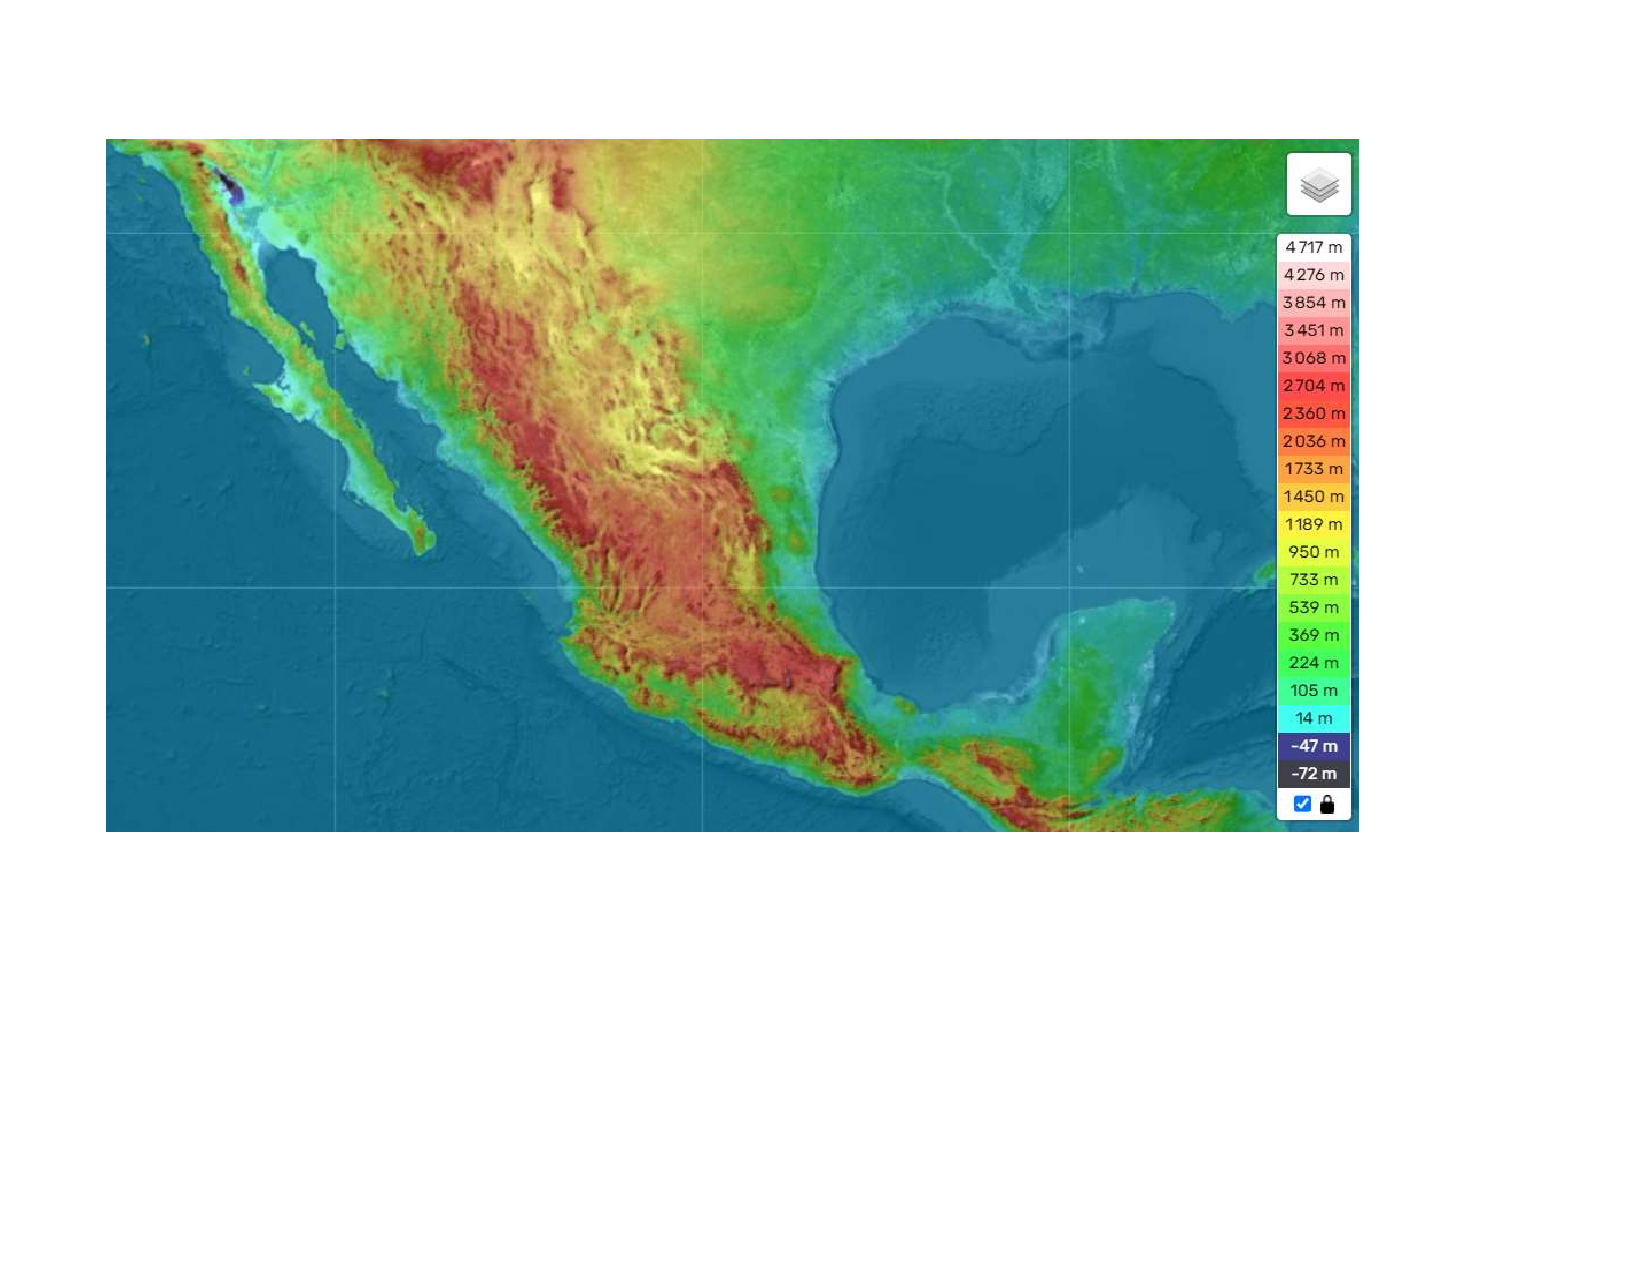
\includegraphics[scale=0.57]{Capitulo3/figs/altitud mexico_cropped.pdf}
\caption{Altitud de México. de: mx.topographic-map.com}
\label{fig: Altitud de México}
\end{figure}

La Universidad Politécnica Metropolitana de Hidalgo (UPMH) se encuentra en el Municipio de Tolcayuca, estado de Hidalgo, México. La elevación de la zona es de $2,336 m$ respecto al nivel del mar. Considerando el techo de servicio a una altura de $120 m$ se establece una altitud geométrica de $2,456 m$, y una altura crucero de $90m$ para una altitud geométrica de $2,426 m$. Ver Figura \ref{Definición de altitudes}.

\begin{figure}[!h]
\centering
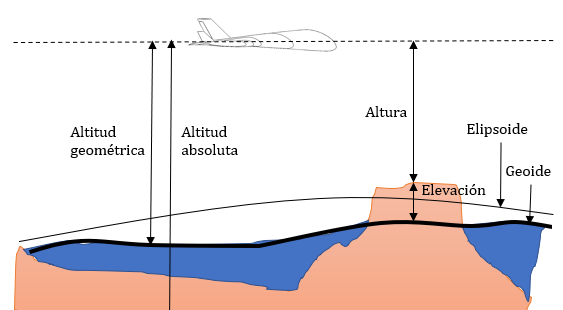
\includegraphics[scale=0.98]{Capitulo3/figs/3 4.png}
\caption{Definición de altitudes}
\label{Definición de altitudes}
\end{figure}

A continuación se establecen las propiedades del aire (temperatura, presión y densidad) en función de la altitud y de acuerdo con la Atmósfera Estándar Internacional\footnote{International Standard Atmosphere o ISA, por sus siglas en inglés}

\medskip

\textbf{Atmósfera Estándar Internacional}

La atmósfera terrestre es un sistema dinámico cambiante cuyo comportamiento queda descrito por la presión, la densidad y la temperatura. 
%
Estas variables cambian con la latitud, longitud, altitud, momento del día, estación anual, etc. 
%
Considerar estas variaciones y dependencias durante el diseño de una aeronave o en las estimaciones de sus actuaciones es algo irrealizable e impracticable. 
%
El objetivo de atmósfera estándar es proporcionar una referencia común para determinar como cambian las magnitudes que describen el comportamiento del aire en función de la altitud. 

Solución en la troposfera \cite{franchini2013}\\
Definimos la altitud en metros con la variable $z$. La distribución de la temperatura $T(z)$ viene fijada por la atmósfera estándar en base a la información experimental recopilada, por lo que el problema queda reducido a las incógnitas de presión $p(z)$ y densidad $\rho(z)$.
Estas ecuaciones se obtienen de los modelos matemáticos que describen el comportamiento físico y termodinámico del aire, que son: la ecuación de estado de los gases ideales y la ecuación del equilibrio de fuerzas.
%
La capa de la troposfera va desde la superficie terrestre ($z=0km$) a nivel del mar hasta una altitud de $z=11km$. La variación de la temperatura se expresa de manera lineal en función de la altitud tal que: $T(z)=T_0 + \lambda z$, dónde $T_0 = T(z=0)=288.15 K$ es la temperatura a nivel del mar y $\lambda = -6.5^{-3} \frac{K}{m}$ es el gradiente de temperatura. 

Para calcular la temperatura utilizamos la ecuación:
\begin{equation}
\label{temperatura ISA}
    T = T_0 - \frac{1}{1000} 6.5 z
\end{equation}
La ecuación hidrostática se define:
\begin{equation}
\label{hidrostática}
    dp = -\rho g dz
\end{equation}
La ecuación del gas ideal se define:
\begin{equation}
\label{gas ideal}
    p = \rho R T 
\end{equation}
Diviendo la ecuación \ref{hidrostática} entre \ref{gas ideal} tenemos que:
\begin{equation}
    \frac{dp}{p}=-\frac{\rho g dz}{\rho R T} = - \frac{g}{RT}dz
\end{equation}
para calcular la presión respecto a la altitud, la temperatura se asume estándar y el aire se asume como un gas ideal. 
Introduciendo la ecuación \ref{temperatura ISA} la expresión resulta:
\begin{equation}
    \frac{dp(z)}{p(z)}= - \frac{g}{R} \frac{dz}{T_0 + \lambda z}
\end{equation}
La resolución de este problema consiste en obtener la variación de la presión respecto a la altitud y, dado que se encuentra en un operador diferencial, hay que tomar el operador inverso a la diferenciación, es decir, la integración.
\begin{equation}
\label{integral ISA}
    \int_{p_0}^{p(z)} \frac{dp}{p} = \int_{0}^{z} - \frac{g}{R} \frac{dz}{T_0 + \lambda z}
\end{equation}
El límite inferior de la integral es $z=0$ y el límite superior una altitud arbitraría $z$ menor o igual a $11,000 m$. Resolviendo la integral \ref{integral ISA} tenemos que:
\begin{equation}
    ln (\frac{p(z)}{p_0})= - \frac{g}{R \lambda} ln (\frac{T_0 + \lambda z}{T_0})
\end{equation}
o bien
\begin{equation}
\label{presion ISA}
    p(z) = p_0 (1 + \frac{\lambda z}{T_0})^{(- \frac{g}{R \lambda})}
\end{equation}
dónde, $p_0 = 101,325 Pa$, es la presión a nivel del mar. 

La variación de la densidad respecto la altitud se obtiene introduciendo la ecuación \ref{presion ISA} en \ref{gas ideal} resultando en:
\begin{equation}
\label{densidad ISA}
    \rho(z) = \rho_0 (1 + \frac{\lambda z}{T_0})^{(- \frac{g}{R \lambda} - 1)}
\end{equation}
dónde, $\rho_0 = \frac{p_0}{R T_0} = 1.225 \frac{kg}{m^3}$, es la densidad del aire a nivel del mar. 
\begin{figure}[!t]
\centering
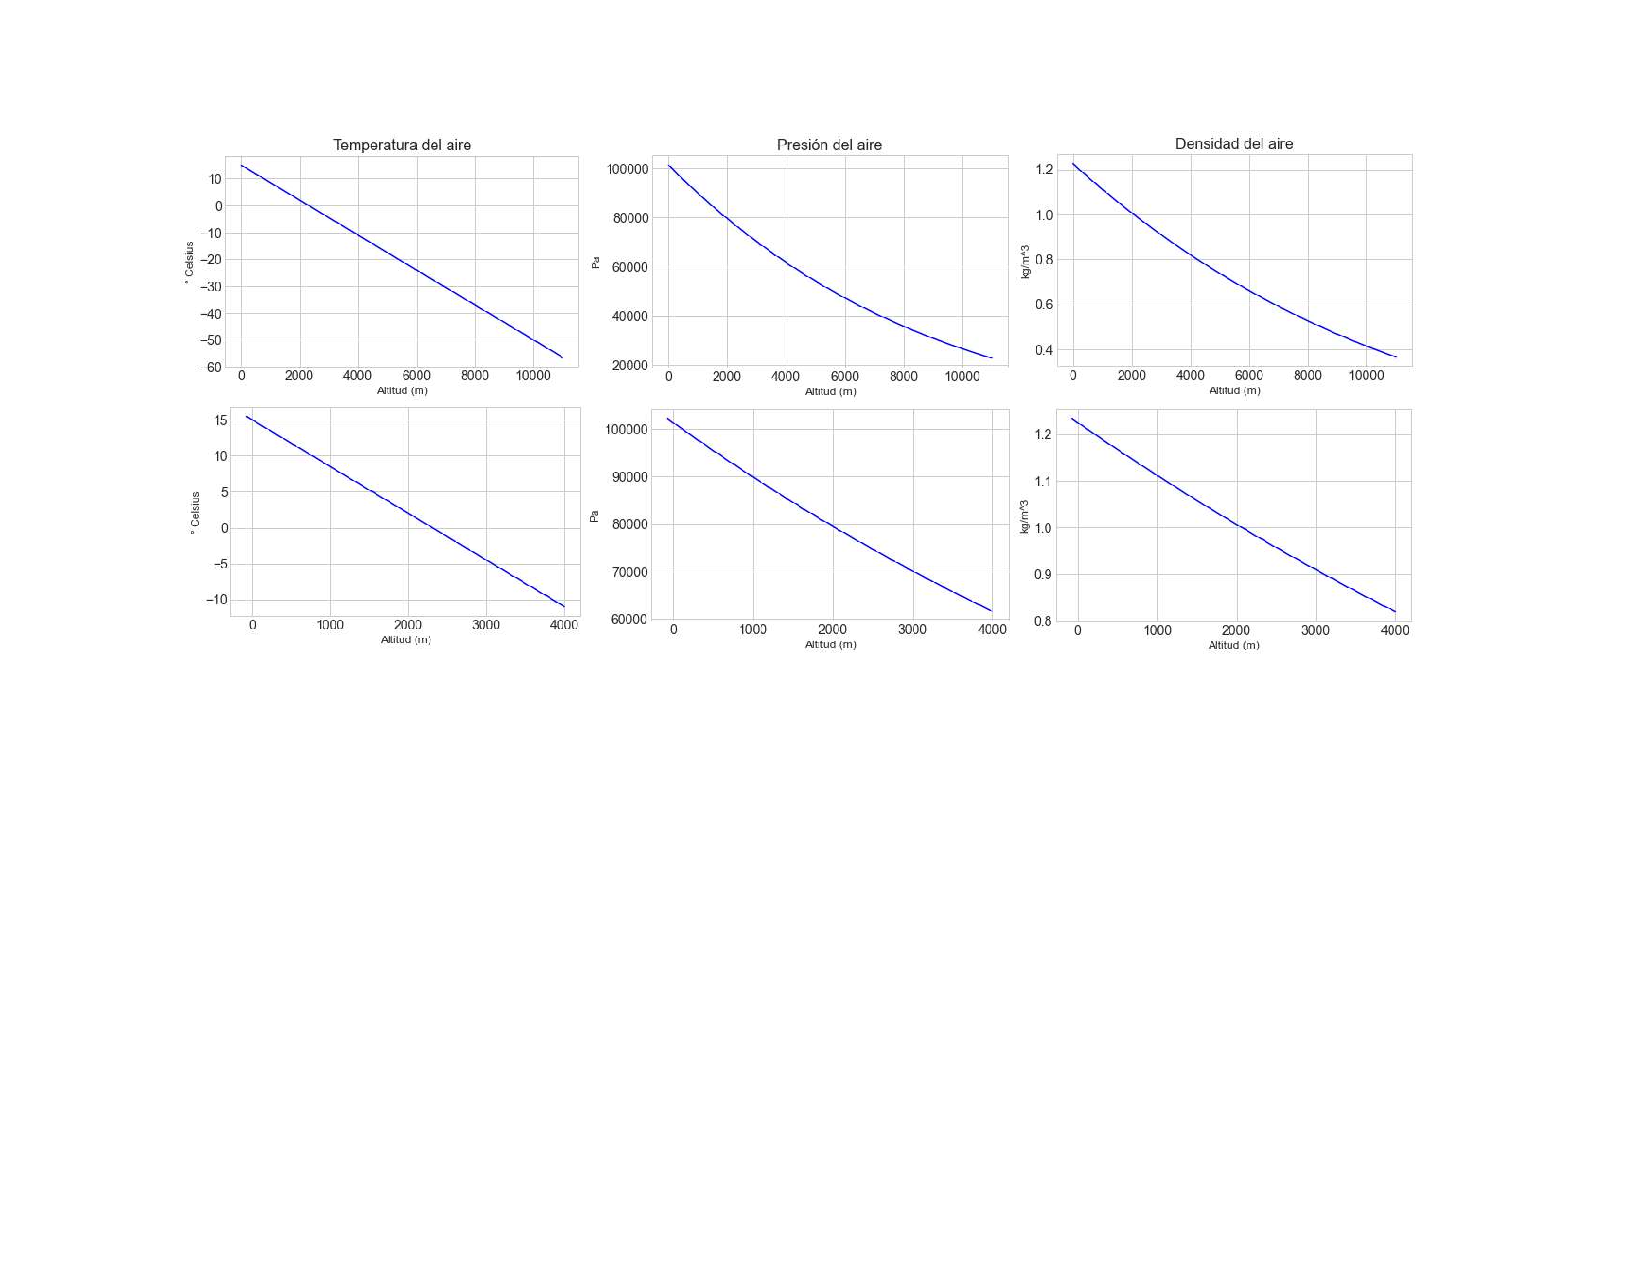
\includegraphics[scale=0.655]{Capitulo3/figs/aire en funcion de altitud_cropped.pdf}
\caption{Temperatura, presión y densidad del aire en función de la altitud en la troposfera (1er fila) y el territorio nacional mexicano (2da fila)}
\label{fig: Temperatura, Presión y Densidad del aire}
\end{figure}
\begin{table}[!h]
\caption{Propiedades del aire en la Universidad Politécnica Metropolitana de Hidalgo de acuerdo con ISA}
\label{tab: Propiedades del aire en UPMH a $z=2,426m$ }
\centering
\begin{tabular}{ |p{9cm}|p{4cm}|  }
\hline
\multicolumn{2}{|c|}{Propiedades del aire en la UPMH para EHEKATL BWB}\\
\hline
Elevación en UPMH,Tolcayuca, Hidalgo, México & $2,336m$\\
Altitud crucero para EHEKATL BWB & $90m$\\
Altitud geométrica crucero en UPMH &  $2,426m$ \\
Temperatura en altitud geométrica & $ -0.77 ^{\circ}C$\\
Presión en altitud geométrica & $ 75,367.8 Pa$\\
Densidad en altitud geométrica & $0.9639 \frac{kg}{m^3}$\\
\hline
\end{tabular}
\end{table}

La Figura \ref{fig: Temperatura, Presión y Densidad del aire} muestra las simulaciones de las ecuaciones \ref{temperatura ISA}, \ref{presion ISA} y \ref{densidad ISA} para el rango de altitud de la troposfera (primer fila) y el rango de altitud del territorio nacional mexicano (segunda fila). 
La Tabla \ref{fig: Temperatura, Presión y Densidad del aire} muestra los datos específicos de acuerdo con la ISA para la ubicación de la UPMH y las altitudes definidas para la misión de vuelo de EHEKATL BWB.

%%%%%%%%%%%%%%%%%%%%%%%%%%%%%%%%%%%%%%%%%%%%%%%%
\section{Diseño Aerodinámico}

Las consideraciones en el diseño aerodinámico de una aeronave de ala-integrada son similares a las de un ala-voladora, ver Tabla \ref{tab: Objetivos Diseño Aerodinámico EHEKATL BWB}. Podemos analizar a EHEKATL BWB como un \textbf{Sistema Aéreo No Tripulado} compuesto de subsistemas integrados por componentes, y estos por partes. 
\begin{table}[!h]
\caption{Objetivos del diseño aerodinámico EHEKATL BWB}
\label{tab: Objetivos Diseño Aerodinámico EHEKATL BWB}
\centering
\begin{tabular}{ |p{4cm}|p{9cm}|  }
\hline
\multicolumn{2}{|c|}{\textbf{Objetivos del diseño aerodinámico EHEKATL BWB}}\\
\hline
\textbf{Generales} & Desempeño,estabilidad y control.\\
\hline
\textbf{Optimización} & Maximizar la sustentación y minimizar el arrastre. \\
\hline
\textbf{Estabilidad estática} & Pendientes negativas en el momento de cabeceo y alabeo; y pendiente positiva en el momento de guiñada. \\
\hline
\textbf{Variables de diseño} & Perfil alar, envergadura y largo, área de referencia, flechado, incidencia, diedro, estabilizadores verticales, aletas de punta, superficies de control aerodinámicas y centro de gravedad. \\
\hline
\textbf{Variables del medio ambiente} & Ángulo de ataque y derrape; velocidad, temperatura, presión, densidad y viscosidad del flujo de aire; número de Reynolds y Mach. \\
\hline
\end{tabular}
\end{table}
Los subsistemas definidos para EHEKATL BWB son: 
sustentación, propulsión, aviónica, estructuras y energía.\\
El \textbf{subsistema de sustentación} en las aeronaves ala-integrada considera la geometría total de la aeronave (superficie sustentadora o área de referencia), y por tanto, a las aeronaves BWB se les clasifica como vehículos de sustentación total. Los componentes del subsistema de sustentación de EHEKATL BWB conllevan la consideración del tipo de perfil alar y geometría para el cuerpo central, ala exterior, estabilizadores de dirección y aletas en la punta del ala. \\
El \textbf{subsistema de propulsión} en aeronaves de ala-integrada ofrece una amplia gama de posibilidades. Como se estableció en la sección de antecedentes y visualmente en la Figura \ref{fig: propulsion distribuida}, podemos ubicar los motores debajo del ala exterior o por encima del cuerpo central, implementar sistemas de propulsión de ingestión de la capa límite y/o sistemas de propulsión distribuida, así como implementar toberas deflectivas que permitan el control de empuje vectorial.
Para la aeronave EHEKATL BWB vamos a establecer dos motores ductofan por encima del cuerpo central. En esta primer versión únicamente se considera el empuje de los motores sin la generación de momentos del TVC. \\
El \textbf{subsistema de aviónica} es esencial para garantizar vuelos íntegros en ala-integrada dada su naturaleza inestable.
%
Las entradas principales al controlador de vuelo son el giroscopio, el acelerómetro y el barómetro; así como el GPS y los receptores de telemetría que permiten obtener información en tiempo real en la estación en tierra. 
En la salida del controlador tenemos: los actuadores (servos-mecanismos) que permiten el movimiento de las ACS, los controladores electrónicos de velocidad que permiten regular la aceleración/desaceleración de los motores, y los motores en sí que dan la fuerza de empuje para alcanzar velocidades que permitan a nuestra aeronave sustentarse y generar maniobras para su navegación. 
%
la tarjeta gráfica y la cámara se consideran la carga útil de EHEKATL BWB.

El \textbf{subsistema de energía} es punto focal en una aeronave de ala-integrada dado que buscamos una aeronave cero emisiones o baja emisiones (dependiendo la aplicación).
%
En la geometría de BWB podemos implementar subsistemas de energía eléctrica, de combustible fósil,de bio-combustibles, de celdas de hidrógeno o híbridos. Esto gracias a que BWB tiene mayor capacidad central que aeronaves tipo TAW, lo que posibilita la implementación de celdas de hidrógeno en el cuerpo central. Los modelos TAW ubican sus tanques de combustible en el ala, lo que para aplicaciones de celdas de hidrógeno sería complejo de implementar.
%
En esta versión de EHEKATL BWB asumiremos baterías eléctricas como subsistema de energía por simplicidad pero cumpliendo con el objetivo de cero emisiones.

El \textbf{subsistema estructural} de un vehículo aéreo no tripulado suele de ser de madera, materiales compuestos entre los cuales destacan las fibras de vidrio y de carbono, también algunas aleaciones o metales. 
El diseño a detalle se encuentra fuera del alcance de este proyecto de tesis.
En la sección de apéndices \ref{superficie alar y potencia requerida} titulada superficie alar y potencia requerida, calculamos el peso vacío en base a una regresión lineal de aeronaves de similar características en dimensión, relacionando con el peso y obteniendo un estimado para este subsistema, condición importante para el resto de cálculos de diseño. 


En este trabajo de tesis para el diseño aerodinámico de EHEKATL BWB se hace uso de los softwares XFLR5 y X-PLANE. Este último en sus extensiones de Airfoil Maker para el diseño de perfiles alares y Plane Maker para el diseño de la aeronave EHEKATL BWB. 

\bigskip
%%%%%%%%%%%%%%%%%%%%%%%%%%%%%%%%%%%%%%%%
\subsection{Selección de Perfiles Alares en XFLR5}
El perfil aerodinámico o perfil alar es la geometría de la sección transversal en una vista lateral de la superficie de sustentación o ala. Los perfiles aerodinámicos \textit{réflex} son perfiles no simétricos que tienen una línea de comba media con doble ligera curvatura en forma de \textit{S}, motivo por el que también son conocidos como perfiles "S", normalmente utilizados en alas-voladoras y alas-integradas. 
De acuerdo con \cite{gatovolante2015}, la característica más significativa de los perfiles réflex es que son perfiles con estabilidad positiva, es decir su coeficiente de momento es siempre positivo salvo y muy ocasionalmente en ángulos de ataque muy elevados, esto se traduce en que el ala con este tipo de perfil vuela en equilibrio sin necesidad de estabilizadores horizontales, por lo que su uso generalizado es en alas tipo delta, alas-voladoras y alas-integradas. 
%
En estas condiciones el centro de gravedad del modelo estará situado en la dirección de la resultante aerodinámica que pasa siempre por el centro de presiones que está determinado por el coeficiente de momento y cofieciente de sustentación. 
%
Se denomina centro de presiones al punto teórico del ala donde se considera aplicada la fuerza de sustentación. 
A efectos teóricos, aunque la presión actúa sobre todo el perfil, se considera que toda la fuerza de sustentación se ejerce sobre un punto en la línea de la cuerda (resultante). La posición del centro de presiones se suele dar en $\%$ de la cuerda del ala desde el borde de ataque. 
%
En el caso de los perfiles auto-estables sitúa el punto de centrado entre el 20 y 25 $\%$ de la cuerda media aerodinámica.
%
Si una perturbación exterior altera la posición del ala, provocando que esta pique, su centro de presiones, se desplaza hacia adelante alejándolo del centro de gravedad, lo que provoca inmediatamente un momento de encabritamiento (morro arriba) que tiende a que el ala recobre su equilibrio inicial. 
%
El principal inconveniente de este tipo de perfiles es que tienen coeficientes de sustentación relativamente bajos mientras que sus coeficientes de resistencia son altos. 
%
Visualmente, las aeronaves con este tipo de perfiles parecen tener el borde de fuga y los alerones ligeramente orientados hacia arriba. Esta geometría es la responsable de generar estabilidad en el momento de cabeceo.
Si utilizáramos un perfil simétrico en lugar de un perfil \textit{réflex} en el diseño de una ala-integrada necesitaríamos una amplia capacidad de deflexión de los elevadores y un complejo sistema de control para un vuelo estable, lo que genera un consumo constante de energía dada la continua deflexión de los efectores, y por tanto, disminuiría el desempeño aerodinámico de la aeronave. 

\begin{table}[!h]
\caption{Perfiles aerodinámicos para generación de conceptos}
\label{tab: Perfiles aerodinámicos EHEKATL BWB}
\centering
\begin{tabular}{ |p{14cm}|  }
\hline
\multicolumn{1}{|c|}{\textbf{Perfiles aerodinámicos para la generación de conceptos}}\\
\hline
LA2573A, UI1720 , FAUVEL 14, MARSKE PIONNER IA, MARSKE XM 1D\\
MH78, MH80, MH91, MH92, MH93\\
NACA 0009, WORTMANN FX 71 120\\
\hline
\end{tabular}
\end{table}
\begin{figure}[!h]
\centering
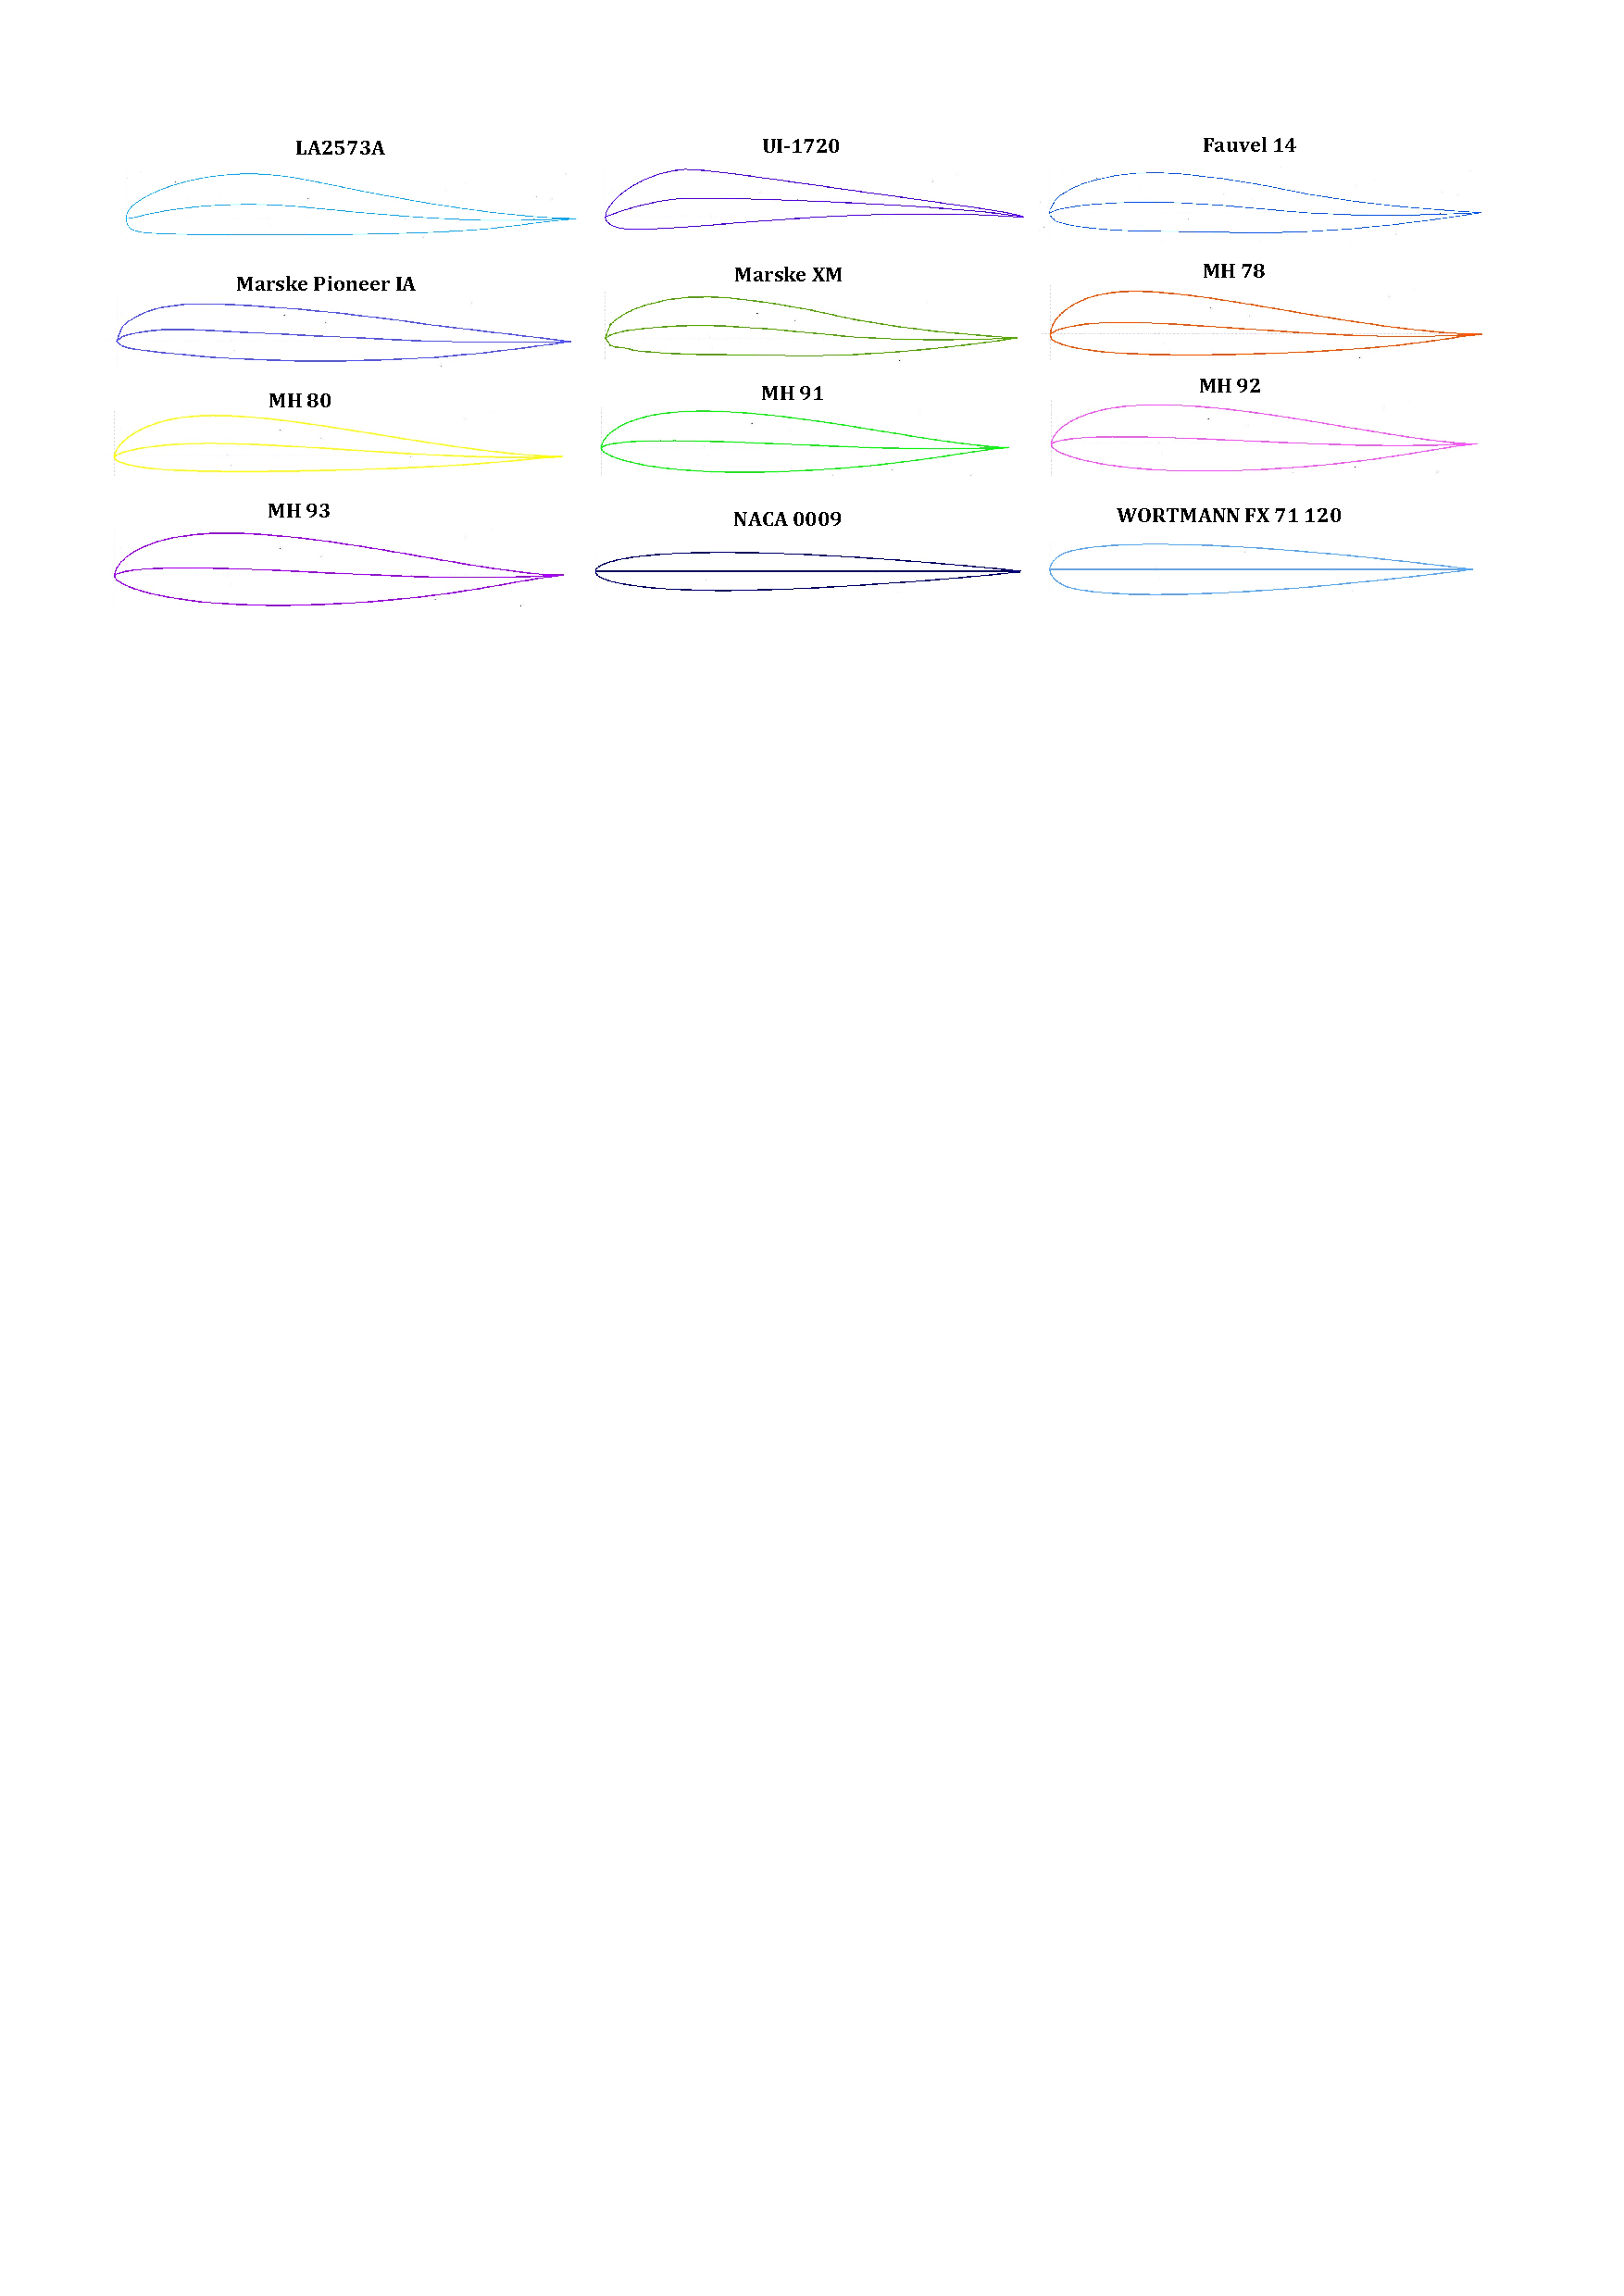
\includegraphics[scale=0.50]{Capitulo3/figs/perfiles aerodinamicos cropped.pdf}
\caption{Perfiles Aerodinámicos}
\label{perfiles aerodinamicos}
\end{figure}

Se seleccionaron los siguientes perfiles para EHEKATL BWB.
\begin{itemize}
    \item \textbf{MH80} en cuerpo central
    \item \textbf{MH78} en ala exterior
    \item \textbf{NACA 0009} en estabilizadores verticales
\end{itemize}

Para contrastar el desempeño de los perfiles seleccionados para EHEKALT BWB, se seleccionaron los doce perfiles aerodinámicos de la Tabla \ref{tab: Perfiles aerodinámicos EHEKATL BWB}. 
%
En la Figura \ref{perfiles aerodinamicos} se muestran las imágenes de los perfiles aerodinámicos de la Tabla \ref{tab: Perfiles aerodinámicos EHEKATL BWB}. Dado que los perfiles seleccionados para EHEKATL BWB son los perfiles MH78 (color amarillo), MH80 (color naranja) y NACA 0009 (color gris) se recomienda poner atención al desempeño de estos perfiles en los resultados del análisis aerodinámico de las Figuras \ref{perfiles aerodinamicos vstall} y \ref{perfiles aerodinamicos vmax} dónde se considero una cuerda de 1m en un régimen de velocidad de 19$m/s$ y 35$m/s$ respectivamente. Se muestran cuatro gráficas en las simulaciones aerodinámicas: coeficiente de sustentación $C_L$ en función del ángulo de ataque $\alpha$, coeficiente de resistencia $C_D$ en función de $\alpha$, polar $C_L / C_D$ en función de $\alpha$ y coeficiente de momento de cabeceo $C_m$ en función de $\alpha$.
%
Tres de los perfiles anteriores no son perfiles réflex. Hablamos de UI-1720, NACA 0009 y WORTMANN FX 71 120. 
%
El perfil aerodinámico UI-1720, fue seleccionado por su alto coeficiente de sustentación y bajo coeficiente de arrastre. Sin embargo, dado que la comba del borde de fuga no cumple con el criterio de perfiles réflex, el coeficiente de momento de cabeceo no satisface con los requerimientos de estabilidad, indispensable en el diseño de alas-voladoras y alas-integradas. Se considera este perfil para contrastar la eficiencia aerodinámica del resto de perfiles réflex.
%
En el caso de los perfiles NACA 0009 y WORTMANN FX 71 120, ambos son perfiles simétricos. El objetivo de lo estabilizadores verticales es brindar estabilidad lateral-direccional al vehículo aéreo, por tal motivo se seleccionan perfiles simétricos para estos estabilizadores que portan los timones de dirección.
%
En la Figuras \ref{perfiles aerodinamicos vstall} y \ref{perfiles aerodinamicos vmax} se muestra a la derecha el color representativo de cada perfil. Cada perfil tiene su nombre y una descripción similar a \textit{T1 Re0.19 M0.06 N9.0}, dónde \textit{T1} es el tipo de simulación (líneas continuas respecto $\alpha$), $Re0.19$ para el número de Reynolds que en este caso es de 0.19, $M0.06$ para un Mach de 0.06 y $N9.0$ representa $N_{crit}$ igual a 9.0 para un flujo laminar. 

\begin{figure}[!h]
\centering
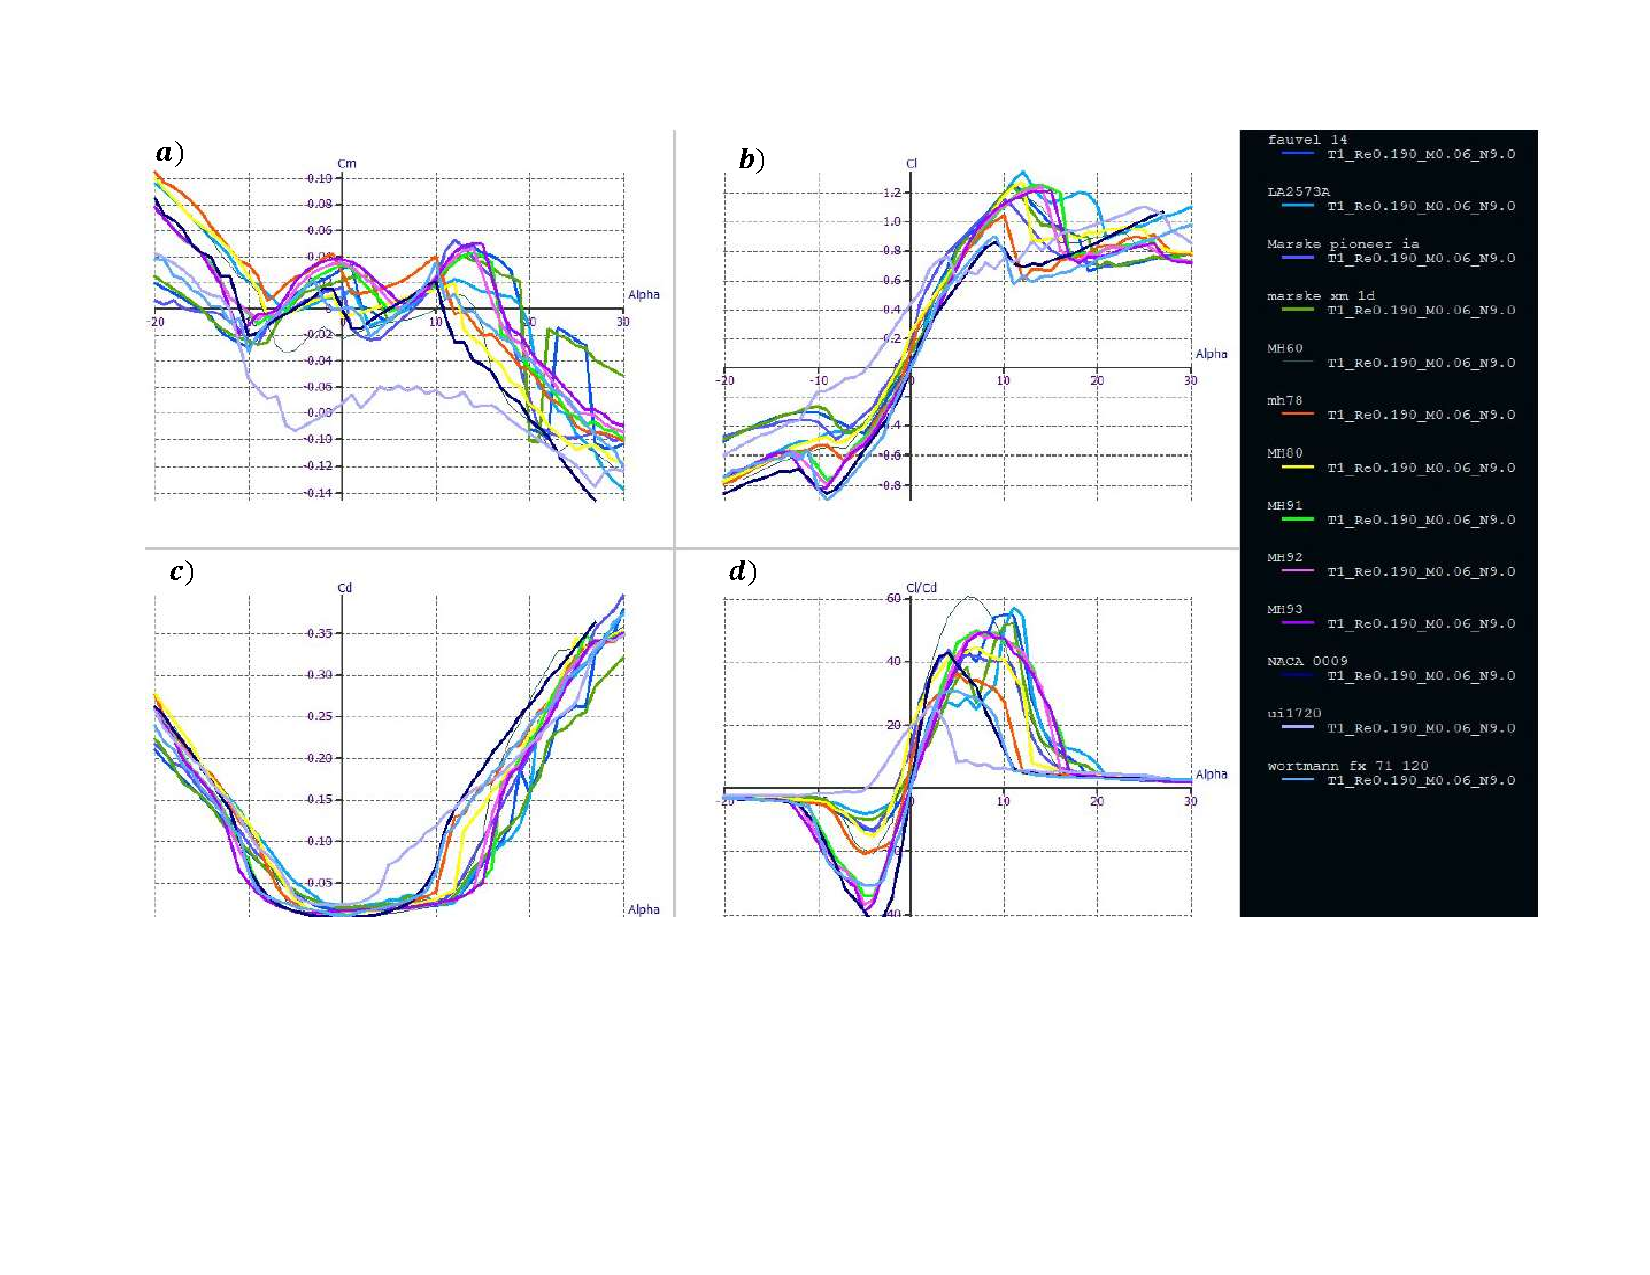
\includegraphics[scale=0.58]{Capitulo3/figs/perfiles 19ms_cropped.pdf}
\caption{Análisis de Perfiles Aerodinámicos.Velocidad de Pérdida: $19 m/s$,Re: $1.9^6$, Mach: $0.055$}
\label{perfiles aerodinamicos vstall}
\end{figure}


\textbf{Análisis de Resultados de Perfiles a 19m/s.} La Figura \ref{perfiles aerodinamicos vstall} muestra el análisis aerodinámico de los perfiles a una velocidad de 19m/s. De acuerdo con la gráfica a) se observa que los perfiles MH80 y MH78 se mantienen cercanos a cero pero con un margen positivo en $C_m$. El perfil MH78 mantiene un margen positivo en todo el rango de $\alpha$ de interés, que va desde -10$^\circ$ hasta 10$^\circ$, mientras MH80 tiene algunos valores negativos en este rango. Ambos perfiles cumplen con el criterio de estabilidad para el cabeceo, pero MH78 demuestra un mejor desempeño en este rubro. En la gráfica b) se observa que el perfil MH80 es de los perfiles con mejor $C_{L_{max}}$, con un valor de 1.25 para un $\alpha$ de 14$^\circ$. El perfil MH78 en su lugar tiene un $C_{L_{max}}$ de 1.03 con un $\alpha$ de 10$^\circ$. En la gráfica c) los perfiles MH78 y MH80 muestran valores altos en $C_D$ respecto a los otros perfiles para esté régimen de velocidad, por tal motivo en la gráfica d) el perfil MH78 muestra una eficiencia de 37 respecto $C_L/C_D$, mientras MH80 muestra una eficiencia de 45. Si bien son valores aceptables, comparado con el resto de perfiles se muestra una eficiencia intermedia para este régimen de velocidad.  

\begin{figure}[!h]
\centering
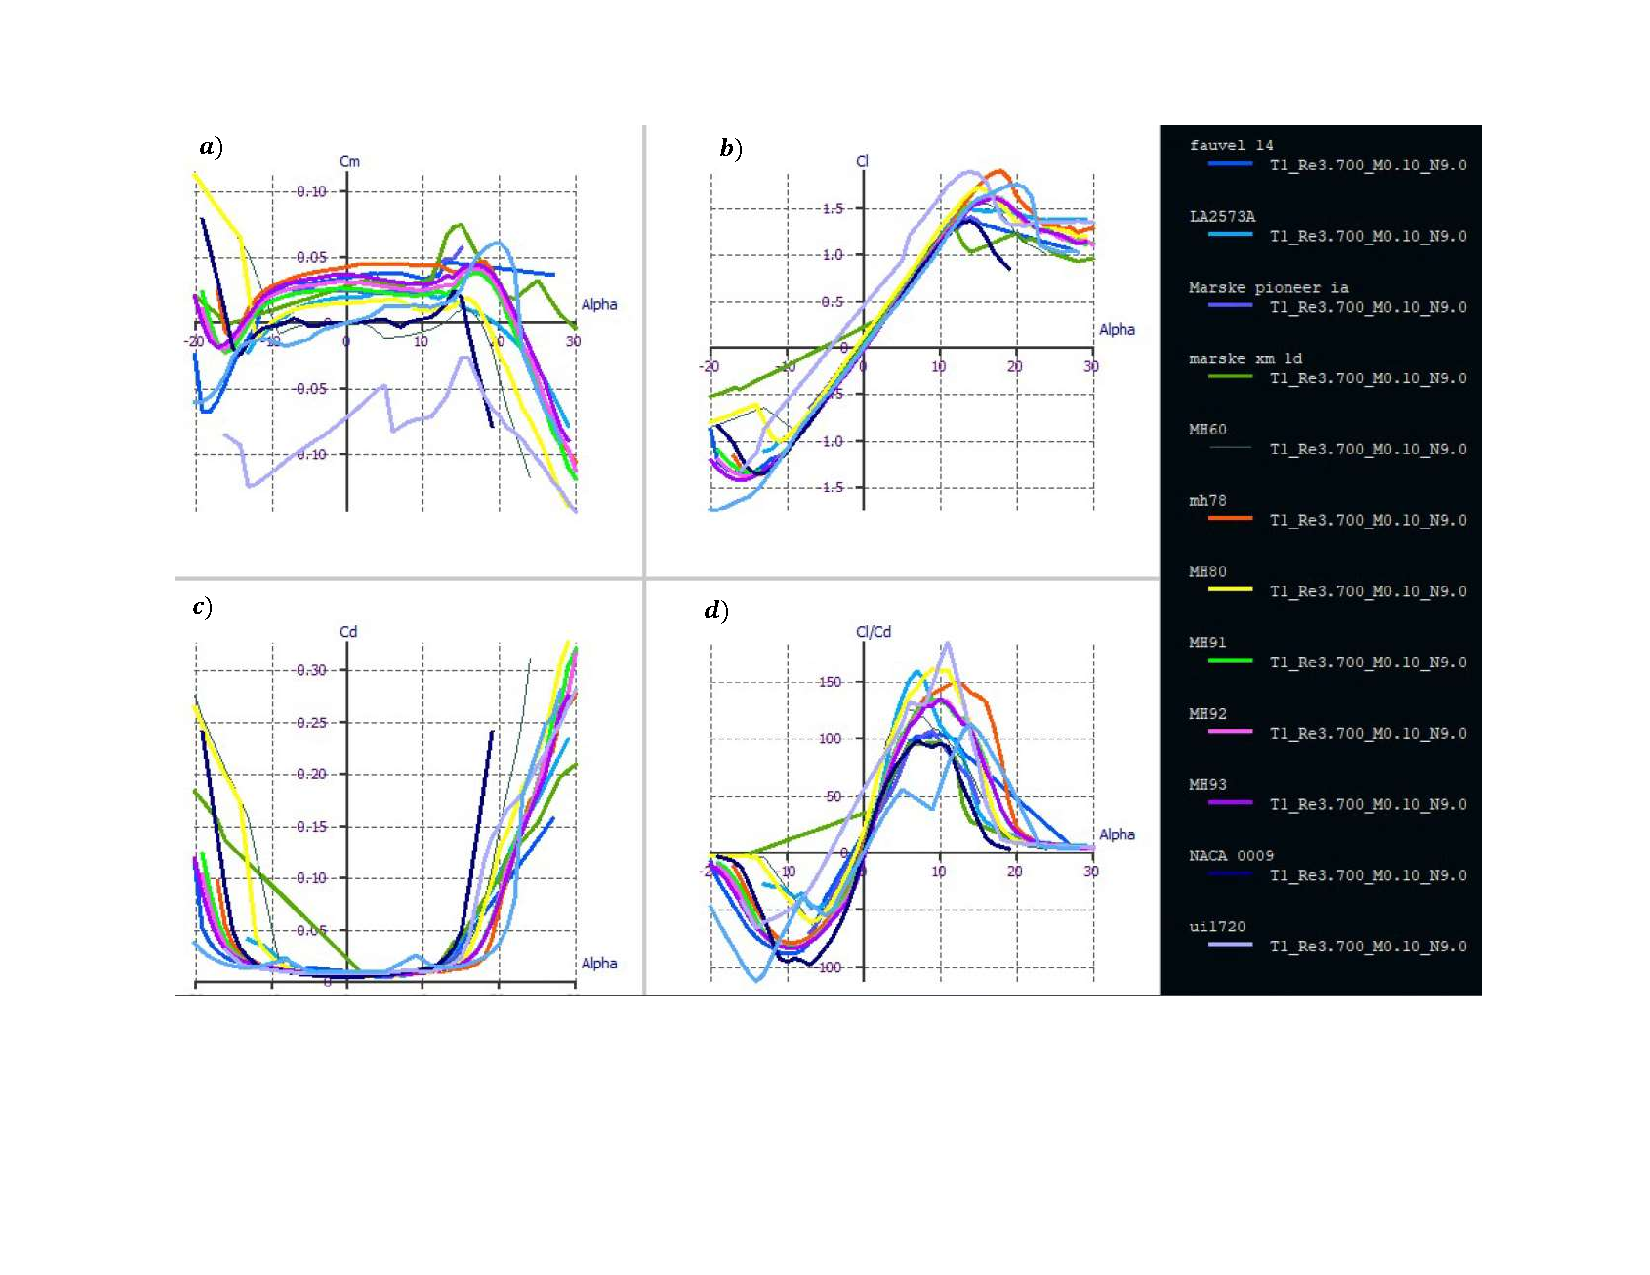
\includegraphics[scale=0.6]{Capitulo3/figs/perfiles 35ms_cropped.pdf}
\caption{Análisis de Perfiles Aerodinámicos.Velocidad de Máxima: $35 m/s$,Re: $3.7^6$, Mach: $0.1$}
\label{perfiles aerodinamicos vmax}
\end{figure}
\textbf{Análisis de Resultados de Perfiles a 35m/s.} La Figura \ref{perfiles aerodinamicos vmax} muestra el análisis aerodinámico de los perfiles a una velocidad de 35m/s. En la gráfica a) se muestra un $C_m$ más estable comparado con el régimen de velocidad de 19$m/s$. Ahora, el perfil MH80 tiene todos sus valores positivos y cercanos a cero en el rango de $\alpha$ de -10$^\circ$ a 10$^\circ$. Por otra parte, MH78 mantiene sus valores positivos, por encima de los valores de MH80 pero menores a 0.05, que también se consideran próximos a cero. En este régimen de velocidad tenemos mejor estabilidad para el momento de cabeceo que en el régimen anterior de 19$m/s$ en ambos perfiles, pero aún MH78 ofrece mejor estabilidad para el momento de cabeceo.
En la gráfica b) se muestra como ahora son los perfiles MH78 y MH80 con el mejor desempeño en $C_L$ después del perfil UI-1720. En criterios de sustentación, nos interesan los valores de $C_L$ desde $\alpha$ igual a 0$^\circ$ hasta el valor de $\alpha$ para $C_{L_{max}}$.  En este criterio, MH78 ofrece un $C_{L_{max}}$ cercano a 2, estando por encima del perfil UI-1720. Por otro lado, MH80 ofrece un buen desempeño con un $C_{L_{max}}$ cercano a 1.7. Aunque el perfil UI-1720 considerado de alta sustentación demuestra valores por encima de ambos perfiles (MH78 y MH80), en términos de $C_{L_{max}}$, MH78 logró un mayor coeficiente y Mh80 está apenas por debajo. 
En la gráfica c) vemos un mejor rendimiento en $C_D$ para ambos perfiles en este régimen de velocidad que el anterior de 19$m/s$. el perfil MH78 demuestra ser uno de los perfiles con menor coeficiente de arrastre, mientras que MH80 también disminuyo estos valores notablemente. 
En la gráfica d) son MH78 y MH80 quienes ofrecen de los mejores desempeños junto con UI-1720 y LA2573A. 
MH80 muestra ligeramente un mejor desempeño que MH78, con valores $C_L/C_D$ por encima de 150, mientras MH78 apenas alcanza 150. Esto debido a que MH80 tuvo un $C_L$ por encima de MH78 en un rango $\alpha$ de 0$^\circ$ a 12$^\circ$, sin embargo el MH78 tiene mejor capacidad al desplome con valores mayores en $C_L$ después del $C_{L_{max}}$.  

El criterio de selección de los perfiles MH78 y MH80 fue debido a su buen desempeño aerodinámico en $C_L$, $C_D$ y $C_L/C_D$, que sobrepasa a la mayoría de perfiles conforme aumenta el régimen de velocidad.
Se selecciona el perfil MH80 para el cuerpo central, dado que esta sección de la aeronave tiene el mayor área de referencia, y MH80 ofrece una mayor razón $C_L/C_D$ desde un $\alpha$ de 0$^\circ$ hasta 12$^\circ$. 
Consecuentemente, se selecciona el perfil MH78 para la sección del ala exterior dado que MH78 ofrece mejores cualidades para la estabilidad en cabeceo y capacidad al desplome.

\medskip

%%%%%%%%%%%%%%%%%%%%%%%%%%%%%%%%%%%%%%%%%%%
\subsection{Diseño de Perfiles Alares en Airfoil Maker}
Airfoil Maker es una herramienta dentro del simulador X-PLANE para diseñar o modificar cualquier perfil alar que nos interese implementar en una aeronave dentro del ambiente de simulación de X-PLANE. El diseño de perfiles aerodinámicos en Airfoil Maker está basado en los coeficientes de sustentación, arrastre y momento de cabeceo. Airfoil Maker permite implementar el comportamiento de perfiles alares para un número de Reynolds específico, y se pueden implementar tantos números de Reynolds como se desee o sea necesario. El software X-PLANE 11 cuenta con una lista disponible de perfiles alares (30 elementos), entre los que se encuentra el perfil NACA 0009.  
En la Figura \ref{Perfiles alares MH80 y MH78 en X-PLANE} se observa el diseño gráfico a base de nodos para alcanzar la geometría de los perfiles MH78 y MH80. Estas geometrías son de refererencia visual y no influyen el comportamiento aerodinámico de los perfiles. 
\begin{figure}[!h]
    \centering
    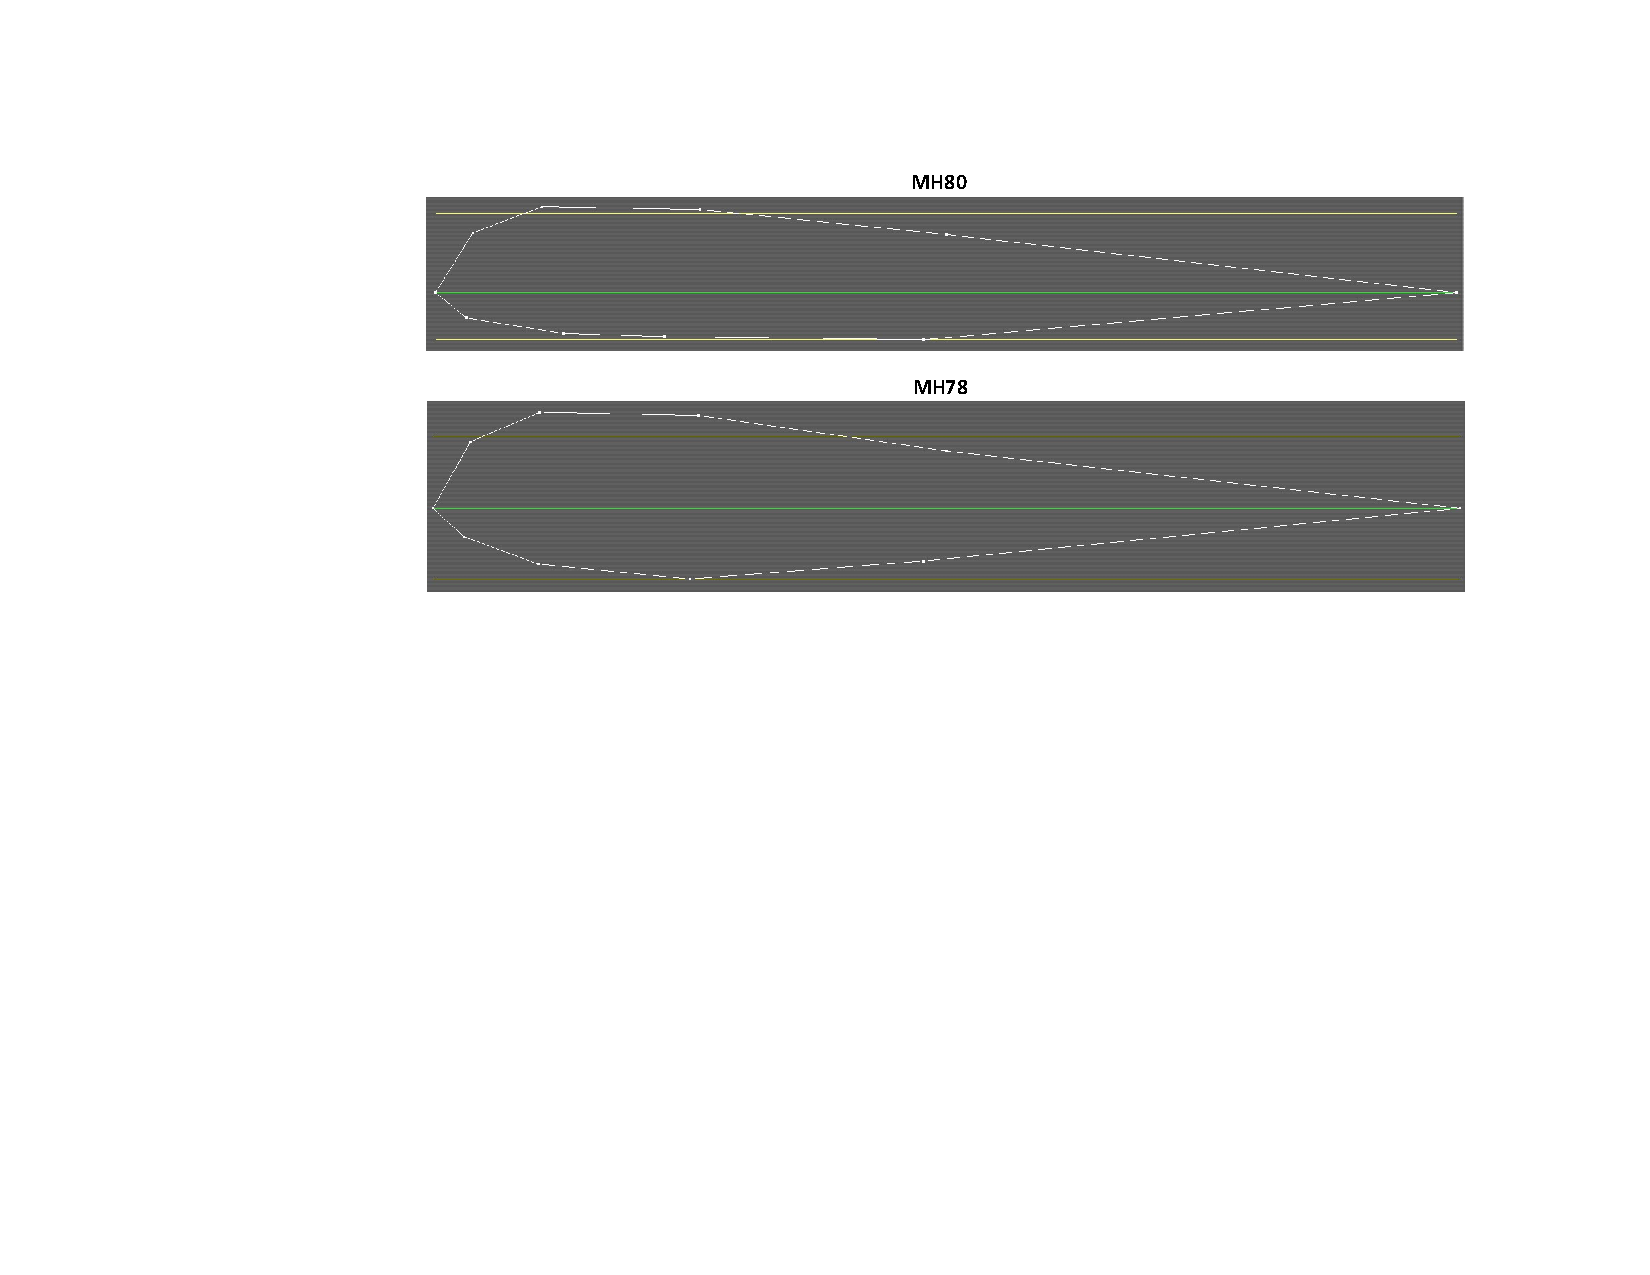
\includegraphics[scale=0.63]{Capitulo3/figs/perfiles xplane_cropped.pdf}
    \caption{Geomtría de perfiles alares MH80 y MH78 en Airfoil Maker}
    \label{Perfiles alares MH80 y MH78 en X-PLANE}
\end{figure}
Para parametrizar los perfiles MH78 y MH80 se utilizan las simulaciones aerodinámicas de la Figura \ref{Desempeño de perfiles réflex MH-78 (azul) y MH-80(rojo)},
\begin{figure}[!h]
    \centering
    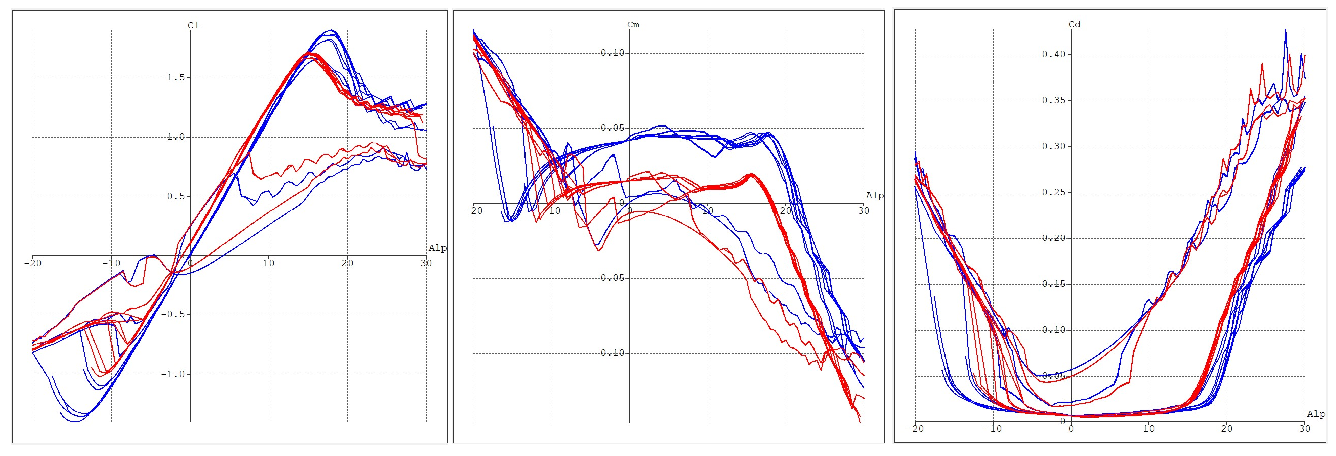
\includegraphics[scale=0.62]{Capitulo3/figs/mh78 y mh80.pdf}
    \caption{Desempeño de perfiles réflex MH78 (azul) y MH80(rojo)}
    \label{Desempeño de perfiles réflex MH-78 (azul) y MH-80(rojo)}
\end{figure}
dónde se muestran simulaciones de los perfiles MH78 y MH80 para números de Reynolds de $10,000$, $100,000$, $1,000,000$ y $4,000,000$.   
%
Bajos número de Reynolds ($10,000$ y $100,000$) muestran un comportamiento de MH78 y MH80 con bajos valores de $C_L$ (menores a 1) y un comportamiento con bastantes no linealidades. En $C_m$ se muestran valores oscilatorios negativos y positivos alrededor del cero (no cumpliendo con el criterio de estabilidad en cabeceo), y los mayores valores en $C_D$ (de 0.1 a 0.4) también con un comportamiento que muestra bastantes no linealidades.
Conforme incrementa el número de Reynolds en el orden de $1,000,000$ a $4,000,000$ se puede observar funciones mejor definidas y con un menor grado de no linealidades. En $C_L$ se muestra una pendiente bien definida así como el $C_{L_{max}}$ (con valores por encima de 1.5). En $C_m$ ambos perfiles conservan valores positivos en el rango de $\alpha$ próximos a cero (lo que garantiza estabilidad en cabeceo) dentro del rango de interés de -10$^\circ$ a 10$^\circ$, y el $C_D$ se mantiene bajo (desde 0.005 hasta 0.15) en un rango de $\alpha$ de -20$^\circ$ a 20$^\circ$.

Para el diseño de los perfiles MH78 y MH80 en Airfoil Maker se seleccionan dos números de Reynolds: $1,000,000$ y $4,000,000$. 
En la Figura \ref{param mh78 airfoil maker} se observa la configuración de la parametrización de los perfiles MH78 y MH80 en Airfoil Maker para los Re de $1e6$ y $4e6$ respectivamente. 
\begin{figure}[!h]
    \centering
    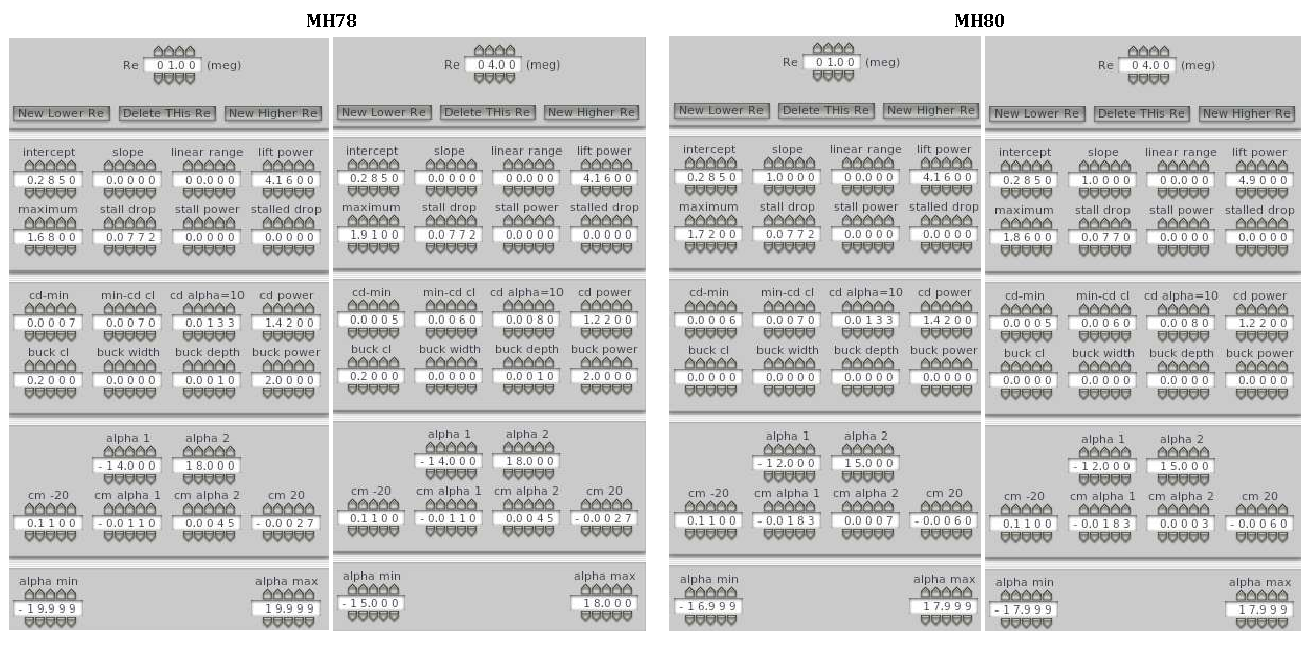
\includegraphics[scale=0.63]{Capitulo3/figs/am mh78 80.pdf}
    \caption{Parametrización de MH78 y MH80 en Airfoil Maker}
    \label{param mh78 airfoil maker}
\end{figure}
La parametrización de lo perfiles en Airfoil Maker se realiza de acuerdo con los cuatro bloques que se aprecian en la Figura \ref{param mh78 airfoil maker}.
En el primer bloque, se ajusta la función de $C_L$ respecto a $\alpha$. 
En el segundo bloque, se ajusta la función de $C_D$ respecto a $\alpha$.
En el tercer bloque, se ajusta la función de $C_m$ respecto a $\alpha$. 
Finalmente, en el cuarto bloque, se ajustan los valores de $\alpha$ min y $\alpha$ para la configuraciones de $C_L$,$C_D$ y $C_m$. 

En la Figura \ref{MH78 en Airfoil Maker} se observan los resultados en términos de los perfiles MH78 y MH80 en Airfoil Maker de acuerdo con la parametrización de la Figura \ref{param mh78 airfoil maker}.
Se muestra en color verde los valores de $C_L$, en rojo los valores de $C_D$ y en amarillo los valores de $C_m$. Las líneas más fuertes o mejor definidas corresponden a las funciones con Re de $4e6$, mientras las más tenues o menos definidas corresponden a las funciones con Re de $1e6$.  
%
Una característica particular de Airfoil Maker es que no restringe la visualización de las funciones aerodinámicas en un rango habitual de ángulo de ataque entre -20 y 30, en su lugar, muestra los $360$ grados. A pesar de esto la parametrización de nuestros perfiles únicamente se basó en un rango máximo de $\alpha$ de -20$^\circ$ a 20$^\circ$.
\begin{figure}[!h]
    \centering
    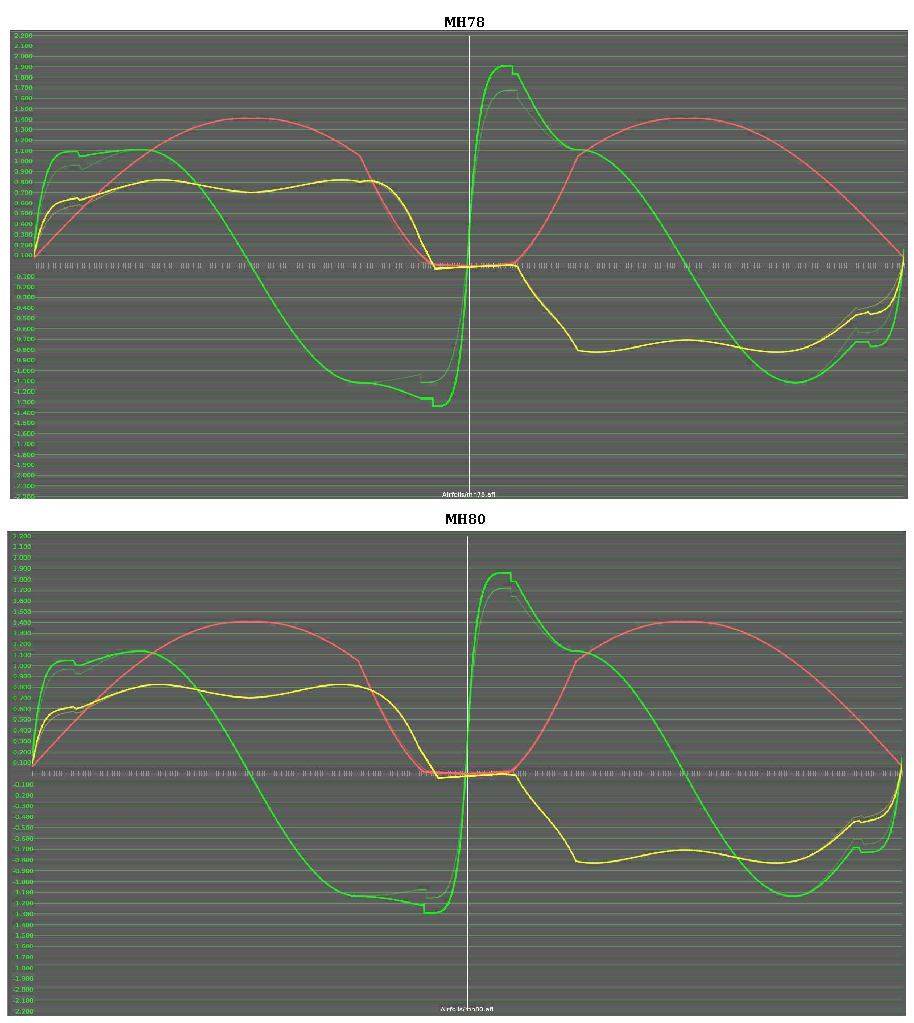
\includegraphics[scale=0.75]{Capitulo3/figs/mh78 80 per.pdf}
    \caption{Desempeño aerodinámico de MH78 y MH80 an Airfoil Maker}
    \label{MH78 en Airfoil Maker}
\end{figure}



%tenemos el intercepto (\textit{intercept}), que refiere al valor de $C_L$ cuando $\alpha$ es cero. La pendiente (\textit{slope}) ajusta la inclinación de la función en un su rango lineal rango que va de -15$^\circ$ a 15$^\circ$ aproximadamente. 
%Con el rango lineal (\textit{linear range}) podemos ajustar este rango de -15$^\circ$ a 15$^\circ$ para incrementarlo o reducirlo. La potencia de sustentación (\textit{lift power}) maneja la curva de los valores próximos a $C_{L_{max}}$, entre mayor potencia, se observa una curva más amplica alrededor de $C_{L_{max}}$. Máximo (\textit{maximum}) representa el valor de  $C_{L_{max}}$. La bajada de desplome (\textit{stall drop}) ajusta la forma de la función $C_L$ en el descenso después del $C_{L_{max}}$. La potencia de desplome (\textit{stall power}) ajusta que tanto va a bajar la función de $C_L$ después de $C_{L_{max}}$.%
%La bajada de desplome (\textit{stalled drop}) determinar la inclinación de la curva después de la bajada de desplome. 

%%%%%%%%%
\subsection{Análisis Aerodinámico con XFLR5}
Ahora, se definen las principales variables del diseño aerodinámico en aeronaves BWB y su impacto en EHEKATL BWB. La Figura \ref{EHEKATL BWB G-33 Vista Isometrica} muestran el diseño geométrico de la aeronave EHEKATL BWB en isométrico.    

\begin{figure}[!h]
    \centering
    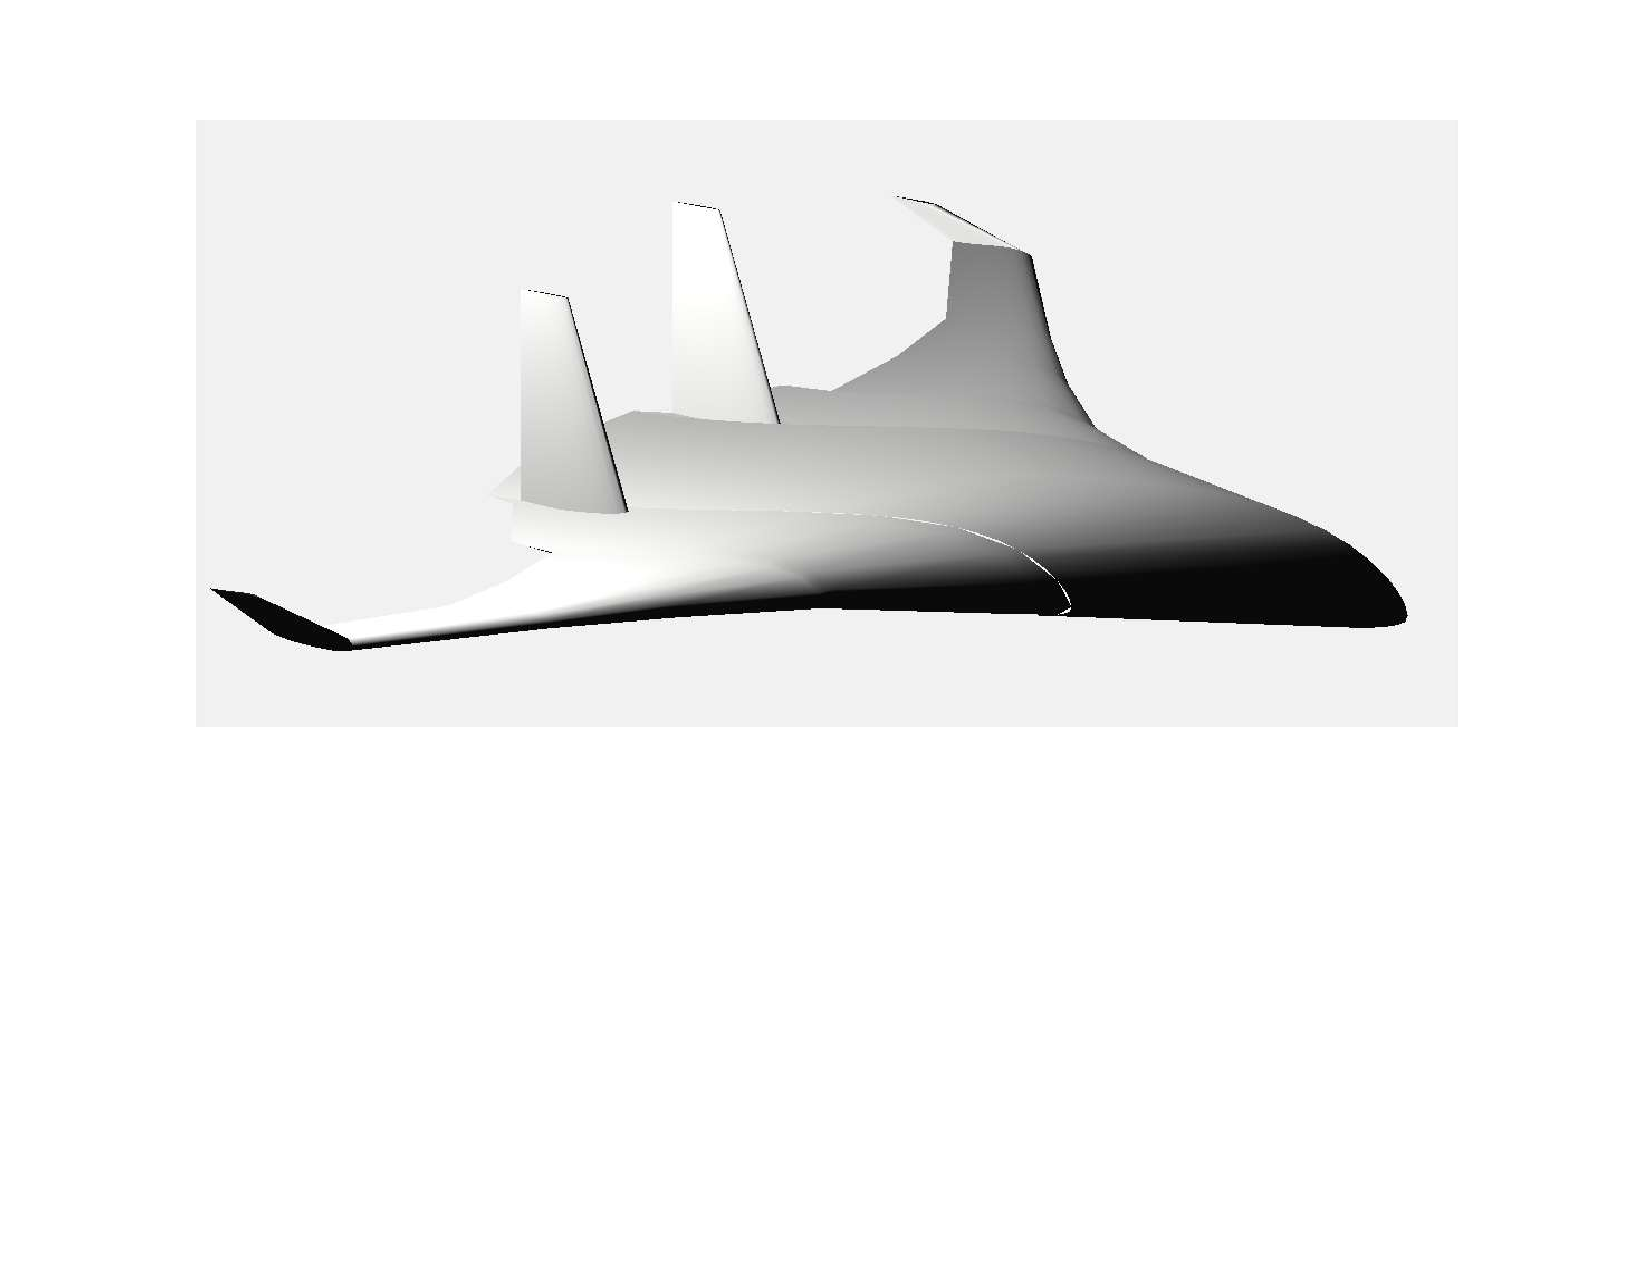
\includegraphics[scale=0.61]{Capitulo3/figs/ehekatl bwb g33 iso_cropped.pdf}
    \caption{EHEKATL BWB - Vista Isométrica}
    \label{EHEKATL BWB G-33 Vista Isometrica}
\end{figure}

%\begin{figure}[!h]
%    \centering
%    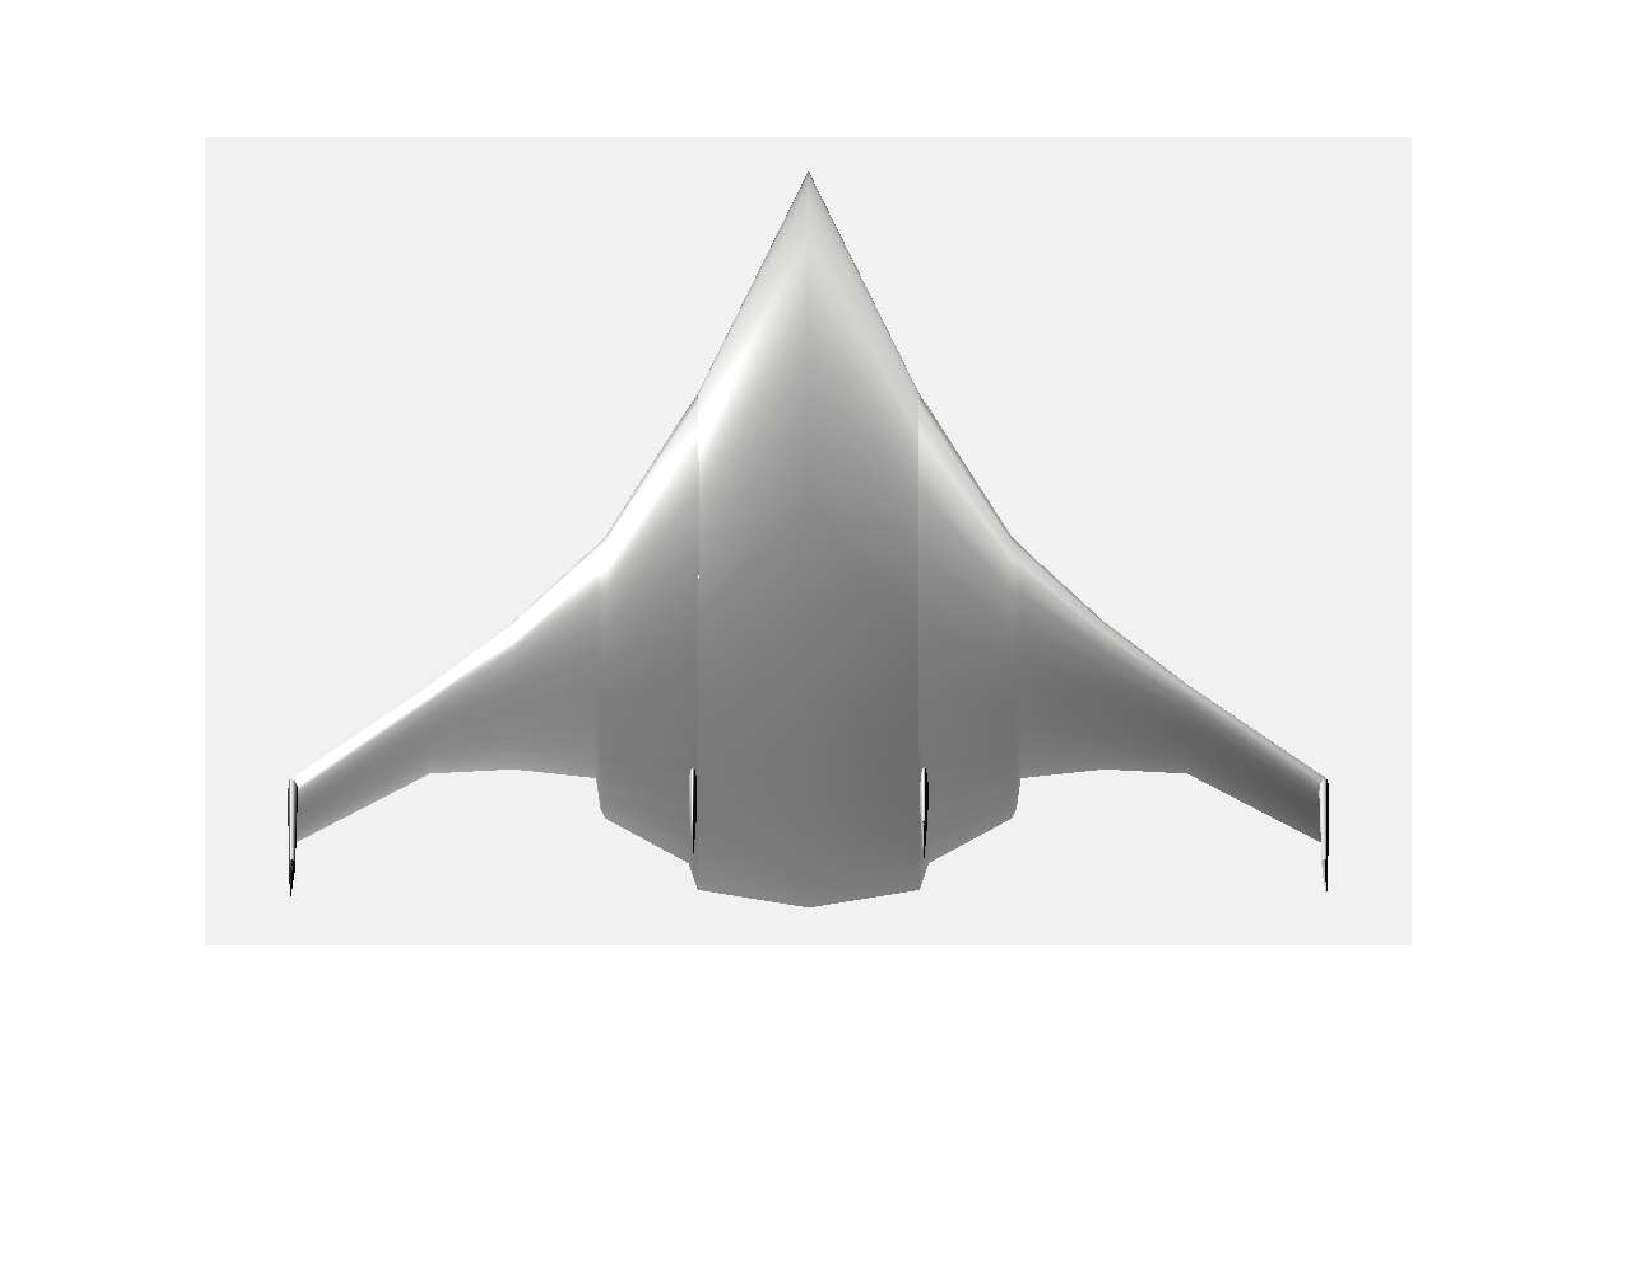
\includegraphics[scale=0.62]{Capitulo3/figs/ehekatl bwb g33 planta 1_cropped.pdf}
%    \caption{EHEKATL BWB - Vista de Planta}
%    \label{EHEKATL BWB G-33 Vista de Planta}
%\end{figure}

\begin{itemize}
    \item \textbf{Ángulo de barrido o flechado.} Se refiere a la inclinación generada hacia atrás del ala con respecto a una línea de referencia (línea central al fuselaje o paralela a esta), ver Figura \ref{EHEKATL BWB G-33 Variables de Diseño} b). Un barrido mayor (por encima de 25$^\circ$) puede mejorar la eficiencia a altas velocidades y reducir la resistencia del aire. Un barrido moderado (igual o por debajo de 25$^\circ$) tiende a ser común en aeronaves TAW,y puede mejorar el rendimiento a velocidades crucero mientras mantiene una estructura robusta. Un ángulo de barrido excesivo puede afectar la distribución del flujo del aire y la estabilidad.  Las aeronaves de ala-voladora YB-49 y y B-2 Spirit cuentan con un flechado de 45$^\circ$ y 55$^\circ$ respectivamente. \textbf{Los ángulos de flechado propuestos para EHEKATL BWB son de 63$^\circ$ en la sección central y 54$^\circ$ en el ala exterior}. 
    \item \textbf{Ángulo de diedro.} Es el ángulo que forma cada semi-ala respecto al plano horizontal, ver Figura \ref{EHEKATL BWB G-33 Variables de Diseño} a). Un ángulo de diedro positivo (alas inclinadas hacia arriba) puede aumentar la estabilidad lateral, ya que tiende a producir un efecto restaurador si la aeronave se inclina lateralmente. En alas-voladoras y alas-integradas, un ángulo de diedro modesto (igual o menor a 5$^\circ$) puede contribuir a una mayor estabilidad lateral y un mejor comportamiento en giros. Es importante resaltar que a mayor estabilidad menor maniobrabilidad, por lo que encontrar un equilibrio respecto a la misión de vuelo es fundamental para garantizar la seguridad e integridad de la aeronave sin recortar substancialmente su capacidad de grados de libertad. \textbf{Se propone un diedro de 3$^\circ$ para EHEKATL BWB}. 
    \begin{figure}[!h]
    \centering
    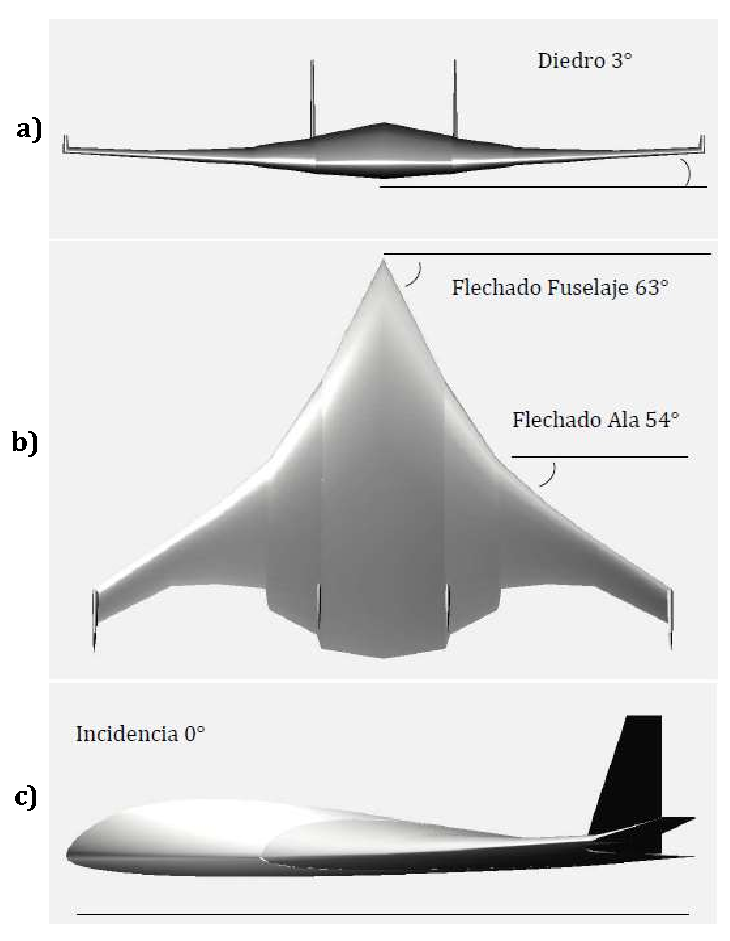
\includegraphics[scale=1.122]{Capitulo3/figs/ehekatl bwb g33 metricas 2.pdf}
    \caption{EHEKATL BWB - Variables de Diseño}
    \label{EHEKATL BWB G-33 Variables de Diseño}
\end{figure}
    \item \textbf{Ángulo de Incidencia.} Es el ángulo que se forma entre la cuerda del ala y la dirección del flujo de aire relativo. Este término suele ser usado a manera de sinónimo para el ángulo de ataque, como variable de diseño, nos referimos al ángulo entre la cuerda del ala respecto a la cuerda del fuselaje central (torsión aerodinámica), ver Figura \ref{EHEKATL BWB G-33 Variables de Diseño} c). Afecta directamente la sustentación generada por el ala y, por lo tanto, el rendimiento del vuelo. Un ángulo de incidencia adecuado es esencial para garantizar una adecuada sustentación y estabilidad en cabeceo. En alas-voladoras y alas-integradas, este ángulo también influye en cómo se distribuyen las cargas aerodinámicas a lo largo de la aeronave. \textbf{La propuesta de diseño EHEKATL BWB en este trabajo de tesis, busca una propuesta minimalista que cumpla con los requerimientos del diseño aerodinámico y se opta por un ángulo de incidencia de cero}. 
    \item \textbf{Estabilizadores Verticales y Aletas en la punta del ala.} Los estabilizadores verticales, también conocidos como derivas, y las aletas en la punta del ala son componentes que influyen en la estabilidad direccional y en el control del balance. En las alas-voladoras y alas-integradas, estos componentes pueden ayudar a mantener la estabilidad en el eje vertical y controlar la deriva lateral. Su diseño, dimensionamiento y ubicación son importantes para asegurar un comportamiento estable y maniobrable, además de un eficiente desempeño aerodinámico. Aunque un área de referencia mayor en estabilizadores verticales y aletas brinda mayor estabilidad direccional también incrementa el arrastre, por lo que es fundamental dimensionar y localizar adecuadamente. \textbf{EHEKATL BWB cuenta con estabilizadores verticales con un área de 0.11 metros cuadrados. Las aletas se diseñaron con el fin de minimizar el efecto vórtice en la punta del ala, así como cuidar la diferencia de presiones entre el intrados y el extrados}. 
\end{itemize}

%\begin{figure}[!h]
%    \centering
%    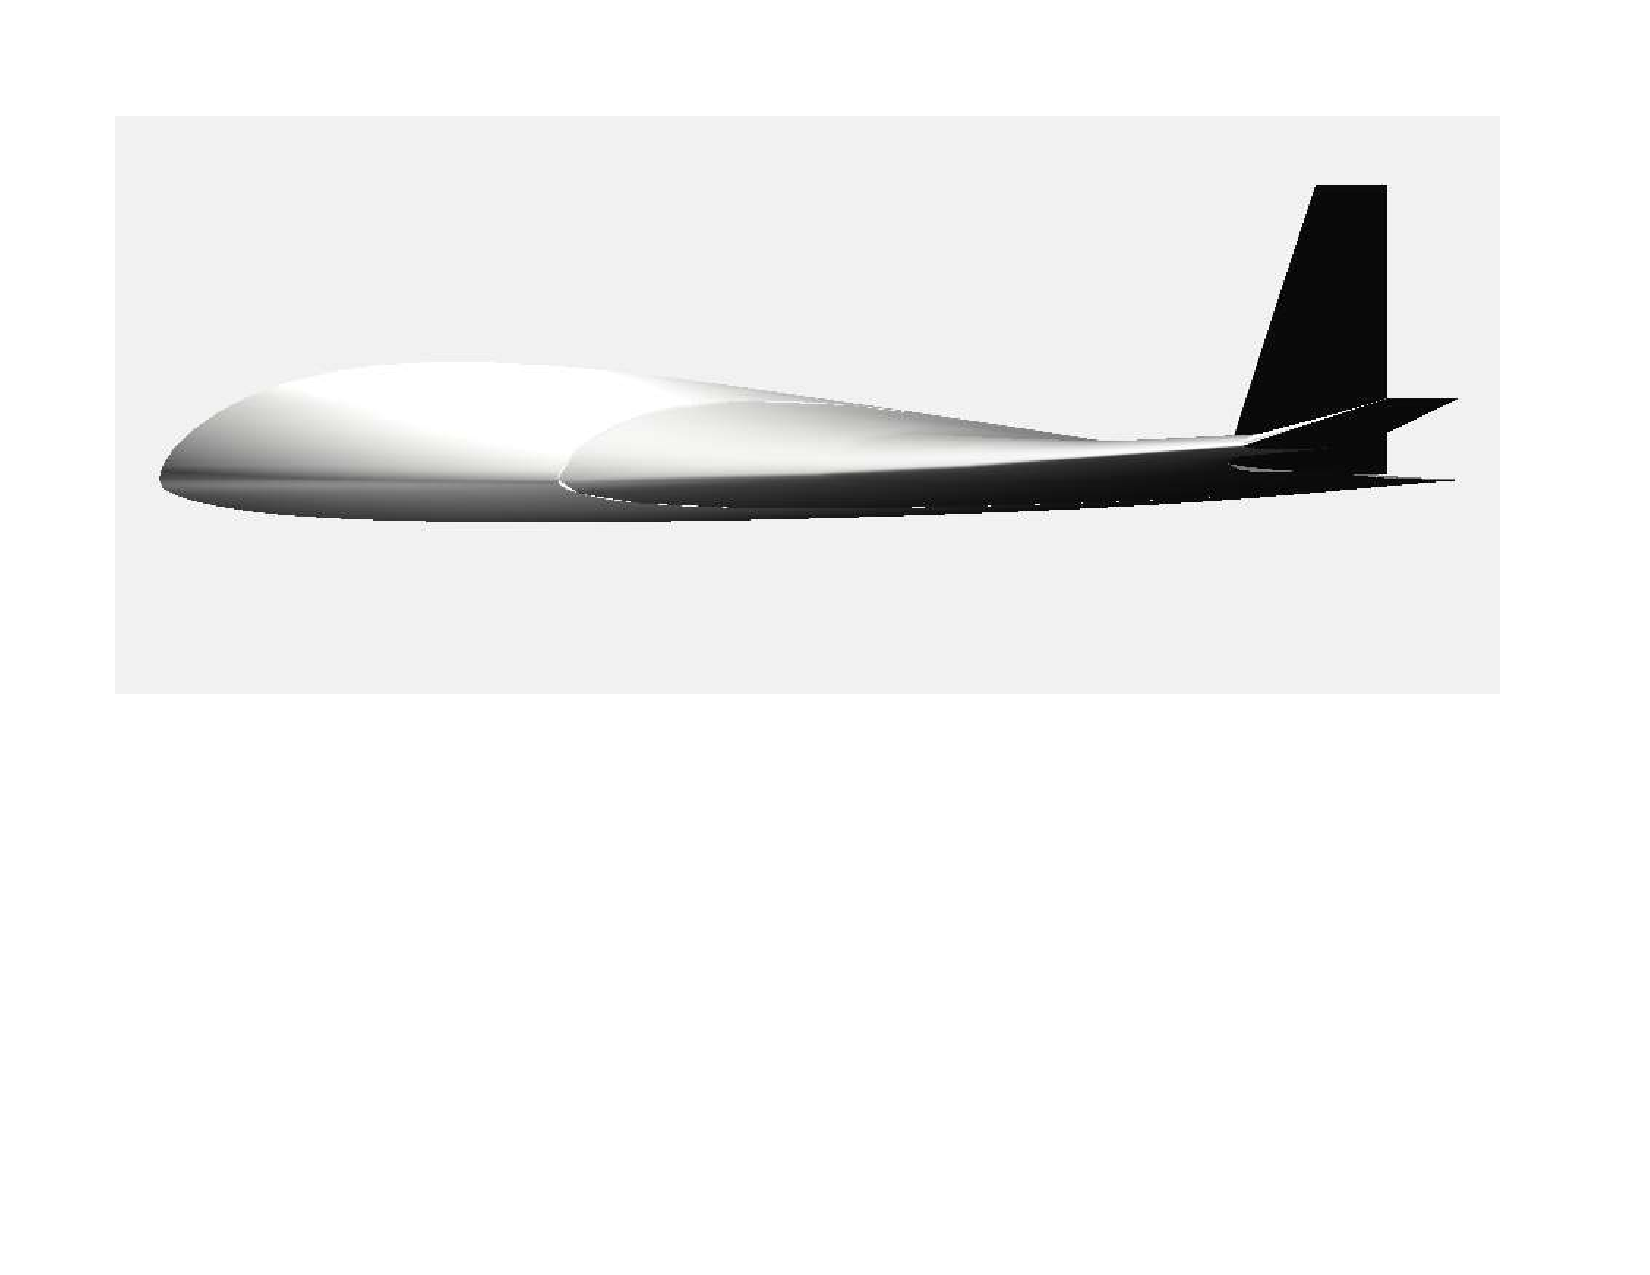
\includegraphics[scale=0.58]{Capitulo3/figs/ehekatl bwb g33 lateral_cropped.pdf}
%    \caption{EHEKATL BWB - Vista Lateral}
%    \label{EHEKATL BWB G-33 Vista Lateral}
%\end{figure}

El borde de fuga de EHEKATL BWB es una geometría particular. Si partimos en vista de planta desde la cuerda central del fuselaje hasta la punta del ala de cualquier semi-ala, podemos apreciar cuatro secciones particulares de tal borde de salida.
\textbf{La primer sección} es la central, dónde se piensan localizar los dos motores por encima, entre los estabilizadores verticales. Propuestas dónde los estabilizadores se integran a la estructura exterior de los motores también son comunes dado que ofrecen un mejor desempeño aerodinámico debido a una menor área frontal entre la integración de estas dos geometrías (motores y estabilizadores verticales).

\textbf{La segunda sección} es para las primeras entradas de control (primeros elevones) que en esta ubicación están pensados para que su función principal sea el momento de cabeceo (elevadores).

\textbf{La tercer sección} es la geometría recta en el borde de fuga del ala exterior. Aquí se localizan dos ACS las cuales están destinadas para las fases de vuelo más interesantes, ya que pueden ofrecer funciones multi-propósito (flaps para aterrizajes y elevons para maniobras en vuelo). 

\textbf{La cuarta sección} es la última con única ACS destinada principalmente al momento de alabeo (alerón). 

Los datos generales del diseño aerodinámico de EHEKATL BWB se muestran en la Tabla \ref{EHEKATL BWB G-33 ficha geometrica}.

\begin{table}[!h]
    \caption{EHEKATL BWB - Datos de Diseño Geométrico}
    \centering
    \begin{tabular}{|c|c|c|c|}
    \hline
    \multicolumn{4}{|c|}{EHEKAL BWB - Diseño Geométrico}\\
    \hline
    Área de Referencia &  $1.4 m^2$ & Envergadura & $2.4m$  \\
    Largo (fuselaje o cuerda raíz) & $1.65m$ & Relación de Aspecto & $3.9$ \\
    Relación de Conicidad & $0.055$ & Ángulo Diedro & $3^\circ$ \\
    Ángulo Flechado Fuselaje & $63^\circ$ & Ángulo Incidencia & $0^\circ$ \\
    Ángulo Flechado Ala & $54^\circ$ & Malla (Paneles) & $644$ \\
    Elevons & $8$ & Timones Direccionales & $2$ \\
    \hline
    \end{tabular}
    \label{EHEKATL BWB G-33 ficha geometrica}
\end{table}

%%%%%%%%%%%%%%%%%%%%%%%%%%%%%%%%%
\textbf{Distribución de masas}\\ 
En la Tabla \ref{Distribucion de masas} se muestran las masas de cada elemento del sistema de aviónica y energía, y la cantidad de cada elemento. 
\begin{table}[!h]
    \centering
    \caption{Distribución de masas}
    \begin{tabular}{|c|c|c|c|}
    \hline
    \textbf{Elemento} & \textbf{Masa (kg)} & \textbf{Cantidad} & \textbf{Masa Total (kg)} \\
    \hline
    Motores & 0.225 & 2 & 0.450 \\ 
    Bateria & 0.259 & 2  & 0.518 \\
    Autopiloto & 0.38 & 1 & 0.38 \\
    Tarjeta gráfica & 0.25 & 1 & 0.25 \\
    Controlador de Velocidad Electrónico & 0.125 & 2 & 0.250 \\
    Tubo Pitot & 0.05 & 1 & 0.05 \\
    Cámara IA & 0.03 & 1 & 0.03 \\
    Servo-mecanismos & 0.021 & 10 & 0.21 \\
    \hline
    \multicolumn{3}{|c|}{ Masa en Vacío} & 4.3\\
    \hline
    \multicolumn{3}{|c|}{Total de Masa en Centro de Gravedad} & 6.438\\
    \hline
    \end{tabular}
    \label{Distribucion de masas}
\end{table}
Con "masa en vacío" se hace referencia al "peso en vacío", haciendo distinción al manejo de masa y no de fuerza en este primer acercamiento. 
Para entender porque se define una masa en vacío de 4.3kg se recomienda ir a la sección de \ref{superficie alar y potencia requerida} \textit{Superficie Alar y Potencia Requerida}.
Es importante recordar que el diseño de vehículos aéreos es un proceso iterativo, por lo que la relación e interdependencia entre las distintas disciplinas y cálculos requiere de actualización y validación para cada iteración. 
La distribución de masas de acuerdo con la geometría de EHEKATL BWB tiene como propósito localizar el centro de gravedad en un lugar estratégico para el desempeño aerodinámico y de estabilidad. 
En EHEKATL BWB la distribución de masas se concentra en dos zonas. En la zona frontal del cuerpo central se localizan el auto-piloto, baterías, carga útil, controladores de velocidad electrócnicos, tubo pitot y cámara. En la zona trasera se localizan los motores y los servo-mecanismos que generan el movimiento de las ACS. Esta distribución localiza el centro de gravedad de EHEKATL BWB G-33 a 0.83m desde el \textit{Datum} o borde de ataque. 


La Tabla \ref{Coordendas de distribución de masas} muestra las coordenadas de la distribución de masas en EHEKATL BWB. 
\begin{table}[!h]
    \centering
    \caption{ EHEKATL BWB - Coordenadas de distribución de masas}
    \begin{tabular}{|c|c|c|c||c|c|c|c|}
    \hline
    \textbf{Descripción} & \textbf{x(m)} & \textbf{y(m)} & \textbf{z(m)} & \textbf{Descripción} & \textbf{x(m)} & \textbf{y(m)} & \textbf{z(m)} \\
    \hline
    Motor 1 & 1.6 & 0.072 & 0.01 & Motor 2 & 1.6 & -0.072 & 0.01 \\
    Bateria 1 & 0.5 & 0.2 & 0 & Bateria 2 & 0.5 & -0.2 & 0 \\
    ESC 1 & 0.5 & 0.069 & 0 & ESC 2 & 0.5 & -0.069 & 0 \\
    Autopiloto & 0.27 & 0 & 0 & Pitot & 0 & 0 & 0 \\
    Tarjeta gráfica & 0.42 & 0 & 0 & Cámara IA &  0.12 & 0 & -0.03  \\
    Serv-elevador 1 & 1.33  & 0.3 & 0 & Serv-elevador 2 & 1.33 & -0.3 & 0\\
    Serv-elevón 1 & 1.3 & 0.55 & 0 & Serv-elevón 2 & 1.3 & -0.55 & 0\\
    Serv-elevón 3 & 1.3 & 0.72 & 0 & Serv-elevón 4 & 1.3 & -0.72 & 0\\
    Serv-alerón 1 & 1.3 & 0.95 & 0 & Serv-alerón 2 & 1.3 & -0.95 & 0\\
    Serv-timón 1 & 1.5 & 0.12 & 0.12 & Serv-timón 2 & 1.5 & -0.12 & 0.12\\
    \hline
    \end{tabular}
    \label{Coordendas de distribución de masas}
\end{table}

Para calcular el centro de gravedad se consideran $n$ puntos de masa $m_i$ con coordenadas ($x_i, y_i, z_i$).  

\begin{equation}
   x_{c} = \frac{\sum_{i=1}^{n} m_i \cdot x_i}{\sum_{i=1}^{n} m_i} 
\end{equation}

\begin{equation}
    y_{c} = \frac{\sum_{i=1}^{n} m_i \cdot y_i}{\sum_{i=1}^{n} m_i}
\end{equation}

\begin{equation}
   z_{c} = \frac{\sum_{i=1}^{n} m_i \cdot z_i}{\sum_{i=1}^{n} m_i} 
\end{equation}

\begin{figure}[!h]
    \centering
    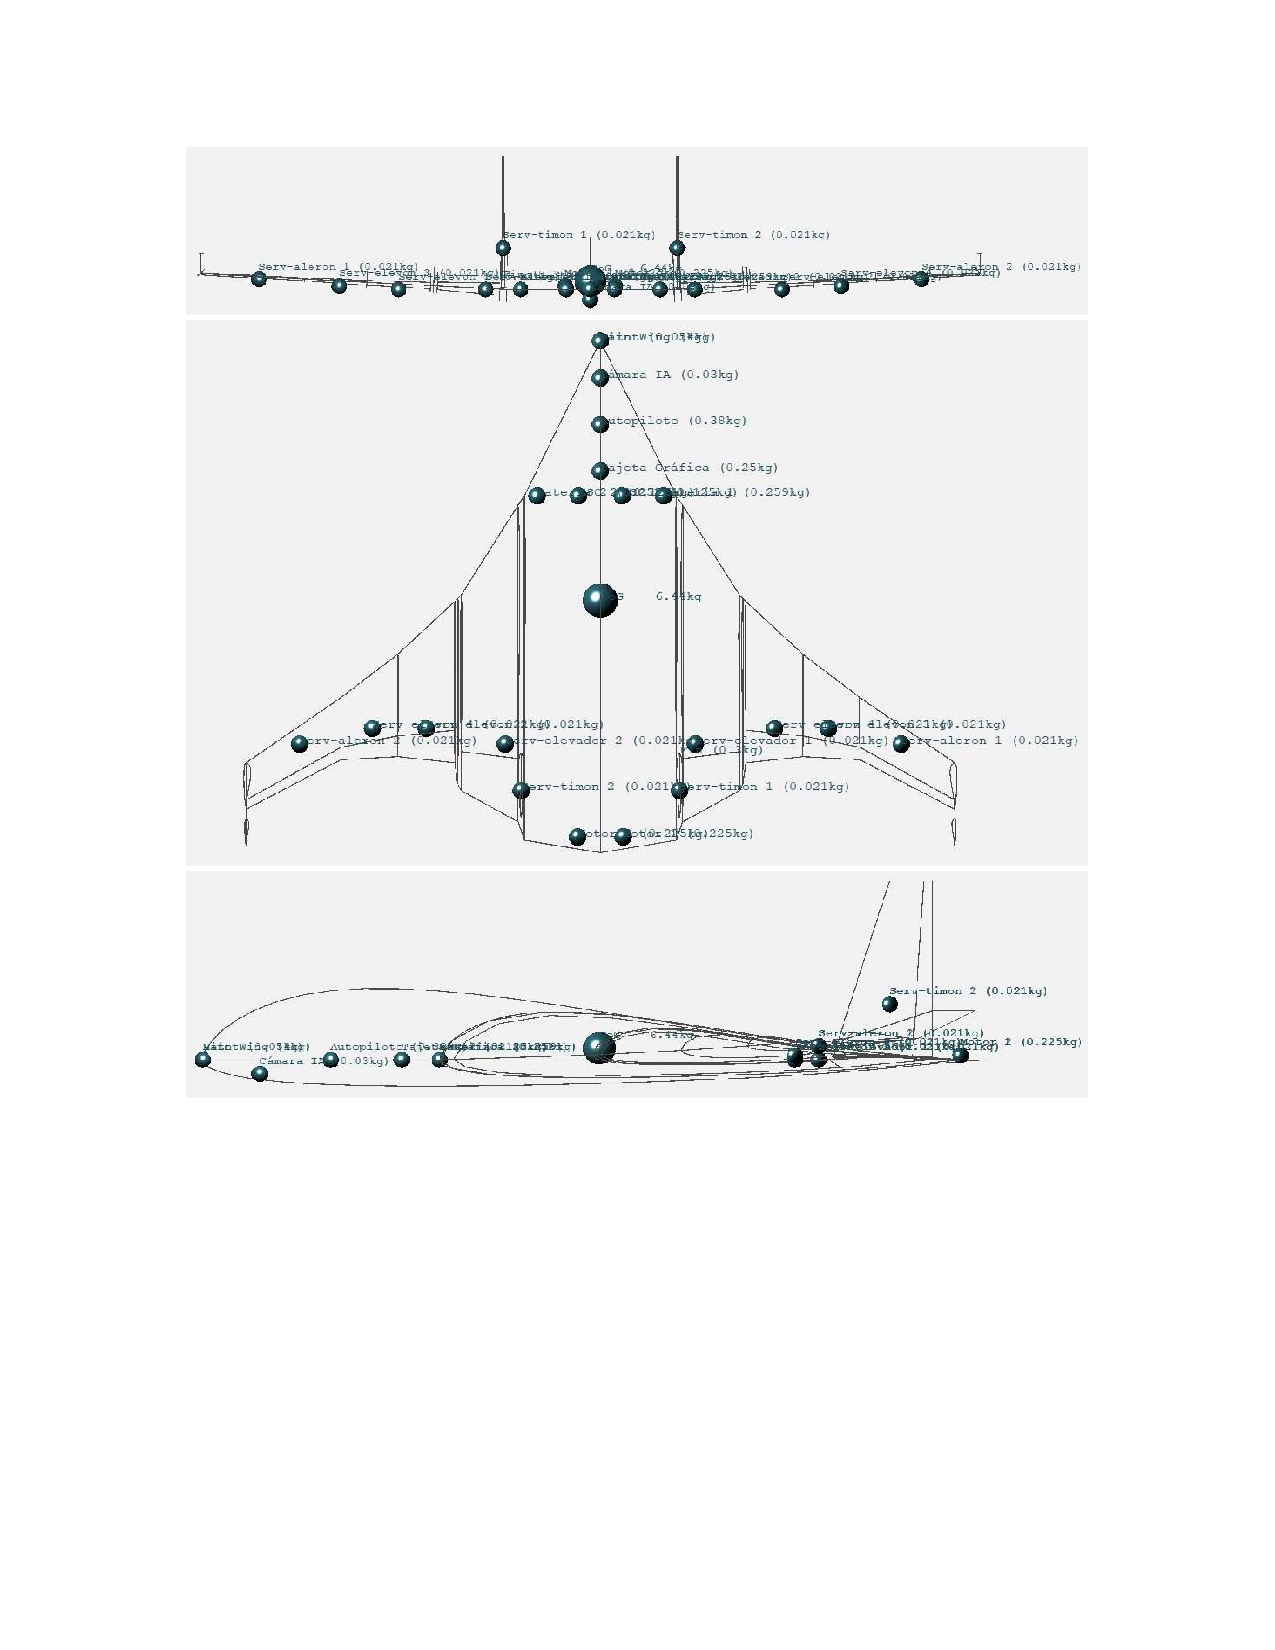
\includegraphics[scale=0.9]{Capitulo3/figs/distribucion de masas_cropped.pdf}
    \caption{Distribución de masas}
    \label{Distribución de masas}
\end{figure}

De acuerdo con los datos de las Tablas \ref{Distribucion de masas} y \ref{Coordendas de distribución de masas} se obtienen los siguientes resultados en el cálculo del centro de gravedad. 
\begin{align}
    x_c &= 0.7473 m \\ \nonumber
    y_c &= 0.0 m \\ \nonumber
    z_c &= 0.0002 m \nonumber
\end{align}
\textbf{El centro de gravedad calculado por XFLR5 arroja las siguientes coordenadas:} $x_C=0.8315$, $y_c=0.0m$ y $z_c = 0.0025$. Las diferencias entre el cálculo analítico y el cálculo con XFLR5 se debe a que en el cálculo analítico únicamente se considera las masas de aviónica y el sistema de energía, mientras XFLR5 además de estas contempla también la localización y masa de los estabilizadores verticales (0.15kg cada uno). La masa en vacío de EHEKATL BWB integra la masa de todo el volumen de la aeronave (cuerpo y estabilizadores) definida en en la sección \ref{superficie alar y potencia requerida}. Si se considera la masa y las coordenadas de los estabilizadores verticales en el cálculo analítico se obtiene la aproximación obtenida con XFLR5. 
En la Figura \ref{Distribución de masas}, se muestra la distribución de los elementos del sistema de aviónica y energía de acuerdo a su masa, y el centro de gravedad como resultante.


\medskip

\textbf{Simulaciones y Parámetros Aerodinámicos}\\
El diseño eficiente y efectivo de aeronaves es un proceso altamente complejo y multidisciplinario que requiere una comprensión profunda de los fenómenos aerodinámicos y fluido dinámicos que influyen en su rendimiento.
Para las simulaciones aerodinámicas de EHEKATL BWB se establecen las velocidades de la Tabla \ref{tab: Re y velocidades} bajo las condiciones ambientales de la Tabla \ref{tab: Propiedades del aire en UPMH a $z=2,426m$ } y que se representan con el tipo de línea en la Figura \ref{Tipo de línea de acuerdo con la técnica de simulación y la velocidad}. 

Antes de analizar los resultados aerodinámicos de EHEKATL BWB es importante recordar que hay tres puntos clave de acuerdo con la distribución de masas,  
 la geometría y las fuerzas aerodinámicas: centro de gravedad (CG), punto neutro (NP) y centro de presiones (CP). 
%
El \textbf{centro de presiones} es el punto resultante de las fuerzas aerodinámicas aplicadas. Depende del modelo aerodinámico y el ángulo de ataque.
%
El \textbf{centro de gravedad} es el punto dónde los momentos actúan, depende solamente de la distribución de masa de la aeronave y no de su aerodinámica.
%
El \textbf{punto neutro} es el punto de referencia dónde el momento de cabeceo no tiene una dependencia del ángulo de ataque. Depende solamente de la geometría externa de la aeronave.
Ahora vamos a definir la estabilidad de la aeronave de acuerdo con la dirección del viento y la relación de posición del centro de gravedad y punto  neutro.
%
Si \textbf{CG por delante del NP} la fuerza de presión en la aeronave coincide con la dirección de la aeronave, pero en sentido contrario. Muy estable.
%
Si \textbf{CG ligeramente por delante del NP} la fuerza de presión en la aeronave coincide con la dirección de la aeronave, pero en sentido contrario. Estable pero sensible a ráfaga de viento.
%
Si \textbf{CG coincide con NP:} La aeronave podría rotar indefinidamente. No estable.
%
Si \textbf{CG por detrás del NP} tenemos estabilidad pero en la dirección contraria, \cite{Deperrois2010}.
%
La Figura \ref{EHEKATL BWB - Centro de Gravedad, Centro de Presiones y Punto Neutro} representa el cambio de posición del centro de presiones de acuerdo con el cambio en el ángulo de ataque a velocidad constante. El centro de gravedad se mantiene constante de acuerdo con la distribución de masas, y el punto neutro se mantiene constante de acuerdo con la geometría de EHEKATL BWB. 
\begin{figure}[t]
    \centering
    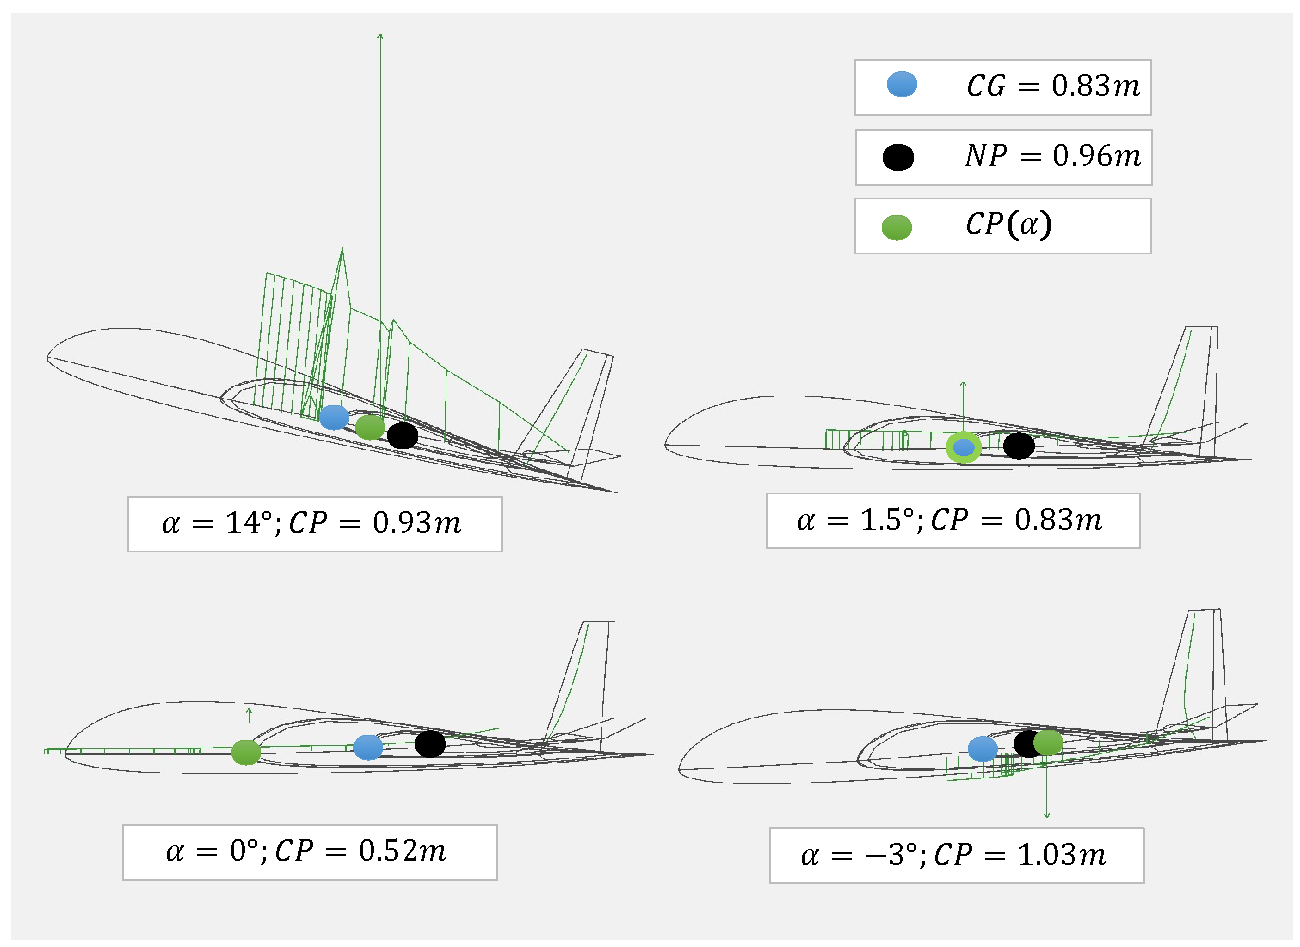
\includegraphics[scale=0.65]{Capitulo3/figs/CG CP NP.pdf}
    \caption{EHEKATL BWB - Centro de Gravedad, Centro de Presiones y Punto Neutro}
    \label{EHEKATL BWB - Centro de Gravedad, Centro de Presiones y Punto Neutro}
\end{figure}

La cuerda aerodinámica media\footnote{Mean Aerodynamic Chord o MAC por sus siglas en inglés} se refiere a la longitud promedio de la sección transversal del ala de una aeronave. Dado que EHEKATL BWB cuenta con ángulos de flechado pronunciados, el cálculo de la MAC es fundamental.
%
La Figura \ref{Desplazamiento del Centro de Presiones de acuerdo la variación del ángulo de ataque} muestra la variación del centro de presiones en relación con el ángulo de ataque. El cálculo de la MAC con XFLR5 es de 0.96m. Se puede apreciar que el centro de presiones tiende a este valor conforme el ángulo de ataque incrementa, y también cuando decrece. Cuando el ángulo de ataque se encuentra entre 0 y -1 se observa un comportamiento asintótico con oscilaciones erráticas. En conclusión, la localización del centro de presiones se aproxima a la MAC conforme el ángulo de ataque aumenta o disminuye, pero en el intervalo mencionado no se define el punto de aplicación para la generación de sustentación. 

\begin{figure}[!h]
    \centering
    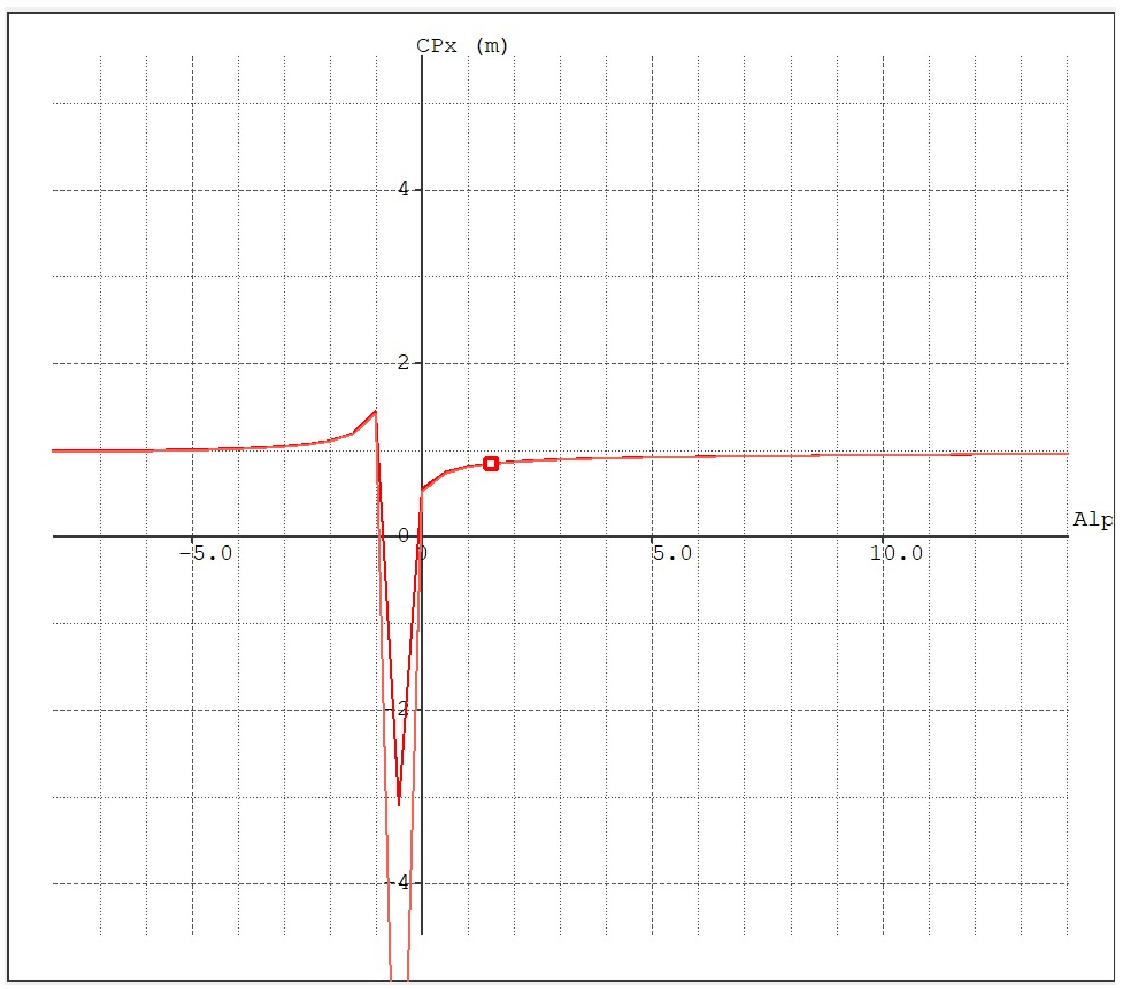
\includegraphics[scale=0.65]{Capitulo3/figs/cp alpha.pdf}
    \caption{Desplazamiento del Centro de Presiones de acuerdo la variación del ángulo de ataque}
    \label{Desplazamiento del Centro de Presiones de acuerdo la variación del ángulo de ataque}
\end{figure}

\medskip

Los \textbf{parámetros de similitud} en el contexto del diseño de aeronaves se refieren a las relaciones dimensionales y de flujo que deben mantenerse constantes entre un modelo a escala y el avión a tamaño real para que los resultados de pruebas en túneles de viento en el modelo a escala sean representativos del comportamiento del avión real.
En este contexto, los dos parámetros de similitud más importantes son el Número de Reynolds (Re) y el Número de Mach. 
Si bien, la escala proporcionada en la Tabla \ref{EHEKATL BWB G-33 ficha geometrica} se considera la escala real para misiones de vuelo en la UPMH, es importante definir el número de Re y de Mach para la conocer la relación dimensional y de flujo de EHEKATL BWB.
%
Los cálculos de los parámetros adimensionales $Re$ y $Mach$ se calcularon a partir de las siguientes funciones. 
\begin{equation}
    Re =  \frac{\rho c V}{\mu}
\end{equation}
\begin{equation}
    Mach = V / a
\end{equation}
dónde $V$ es la velocidad de la aeronave, $\rho$ es la densidad del fluido, $c$ es la cuerda del perfil, $\mu$ es la viscosidad del fluido y $a$ es la velocidad del sonido. Es importante mencionar que la viscosidad varia conforme la temperatura del fluido pero es prácticamente independiente de su presión.

La fórmula para calcular la velocidad del sonido es la siguiente:
\begin{equation}
    a = 331.3 \sqrt{1 + \frac{T}{273.15}}
\end{equation}
Considerando la temperatura $T$ en grados Celsius. 

El rango de velocidades definidas para EHEKATL BWB se muestra en la Tabla \ref{tab: Re y velocidades} respecto al número de Re mínimo y máximo, considerando la cuerda en la punta de la aleta y la cuerda raíz respectivamente. Asimismo, se muestra el número de Mach de acuerdo con las velocidades definidas y las condiciones ambientales de la Tabla \ref{Datos de entrada para simulación en XFLR5 de EHEKALT BWB G-33}, datos de entrada para las simulaciones de la aeronave EHEKATL BWB.   
\begin{table}[!t]
    \centering
     \caption{Velocidades y parámetros de similitud para las simulaciones aerodinámicas de EHEKATL BWB}
    \begin{tabular}{|c|c|c|c|}
    \hline
     \textbf{Velocidad} & \textbf{Reynolds - Raíz} & \textbf{Reynolds - Punta} & \textbf{Mach} \\
     \hline
     \textit{Pérdida} $19 m/s$ & $1,963,213$ & $107,084$  & $0.057$\\
     \textit{Despegue} $22 m/s$ & $2,273,194$ & $123,992$  & $0.066$\\
 \textit{Crucero} $27 m/s$ & $2,789,829$ & $152,163$  & $0.081$\\
     \textit{Máxima} $35 m/s$ & $3,616,445$ & $197,261$  & $0.105$\\
     \hline
    \end{tabular}
    \label{tab: Re y velocidades}
\end{table}
\begin{figure}[!h]
    \centering
    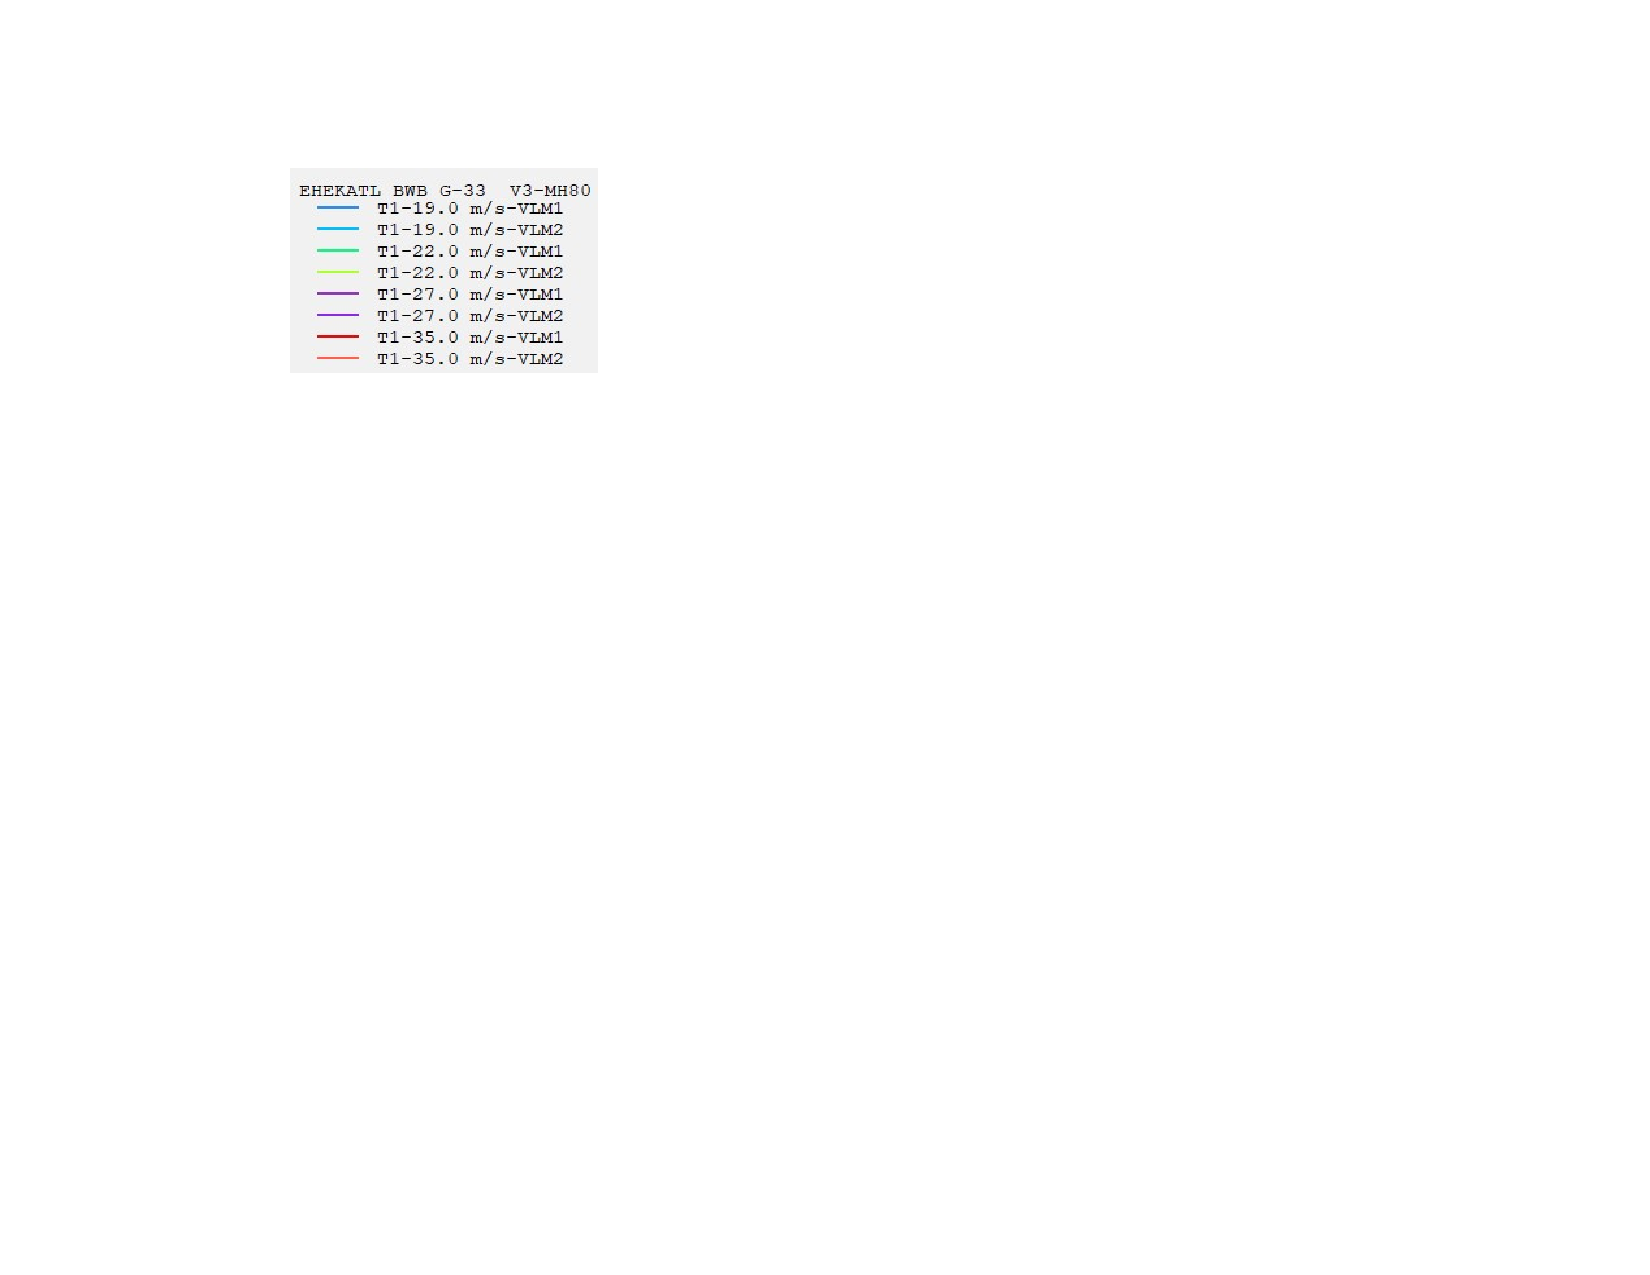
\includegraphics[scale=1.2]{Capitulo3/figs/lineas de simulaciones (1).pdf}
    \caption{Tipo de línea de acuerdo con la técnica de simulación y la velocidad}
    \label{Tipo de línea de acuerdo con la técnica de simulación y la velocidad}
\end{figure}

\begin{table}[t]
    \centering
    \caption{Datos de entrada para simulación en XFLR5 de EHEKALT BWB}
    \begin{tabular}{|c|c|c|}
    \hline
    \multicolumn{3}{|c|}{Parámetros del fluido (aire) en XFLR5} \\
    \hline
    Concepto & Cantidad & Unidad \\
    \hline
    Temperatura & -0.8 & $^{\circ}C$  \\
    Altitud & 2,426 & $m$ \\
    Presión & 75,379.9 & $Pa$ \\
    Densidad & 1.02344 & $kg/m^3$ \\
    Viscosidad Dinámica & $1.63e05$ & $kg/ms$ \\
    Viscosidad Cinemática & $1.59e05$ & $m^2/s$ \\
    Velocidad del Sonido & 330.8 & $m/s$ \\
    \hline
    \end{tabular}
    \label{Datos de entrada para simulación en XFLR5 de EHEKALT BWB G-33}
\end{table}

La cuerda raíz es de $1.65m$, la cuerda en la punta del ala es de $0.15m$ y en la punta de la aleta de $0.9m$.
%
En la Figura \ref{Tipo de línea de acuerdo con la técnica de simulación y la velocidad} se puede apreciar los tipos de línea (colores) de acuerdo al régimen de velocidad y tipo de simulación. Se emplearon las simulaciones VLM1 y VLM2. En la sección de apéndices \ref{Simulaciones con XFLR5} se explican las propiedades de las técnicas de simulación en XFLR5 y sus limitaciones.
Las velocidades establecidas para EHEKATL BWB fueron con el propósito de obtener el mayor rendimiento posible y cumplir con las normativas de la \textit{FAA} para VANTS (Vehículos Aéreos No Tripulados) de escala menor. 
\textbf{La velocidad límite establecida por la \textit{FAA} es de $160km/h$, y la velocidad máxima de EHEKATL BWB es de $126km/h$, aproximadamente el $10\%$ de la velocidad del sonido}.



El \textbf{número de Reynolds} representa la relación entre las fuerzas inerciales y viscosas en el flujo alrededor de un objeto. $Re$ es un valor adimensional a través del cual podemos determinar la naturaleza de la capa límite viscosa, es decir, si el flujo de aire es laminar o turbulento. Cuando dos objetos tienen el mismo número de Reynolds, experimentan patrones de flujo similares, ya sea laminar o turbulento. Esto es crucial en el diseño aerodinámico, tanto del ala como de las superficies de control, donde las propiedades de flujo son esenciales para la eficiencia y el rendimiento.

El \textbf{número de Mach} es crítico para determinar el comportamiento aerodinámico de un objeto en relación con la velocidad del sonido en el medio circundante. Cuando dos objetos o configuraciones tienen el mismo número de Mach, están experimentando condiciones aerodinámicas similares en términos de ondas de choque, compresibilidad y fenómenos asociados con la velocidad del sonido. Esto es esencial para el diseño y la prueba de aeronaves y vehículos espaciales, donde la velocidad y la compresibilidad del flujo son factores cruciales.
Los rangos de interés del número de Mach son
\begin{itemize}
    \item Subsónico : $Mach < 1.0$
    \item Transónico : $0.8 < Mach < 1.2$
    \item Supersónico : $1.0 < Mach < 5.0$
    \item Hypersónico : $5.0 > Mach$
\end{itemize}

La \textbf{compresibilidad} y la \textbf{viscosidad} son dos fenómenos aerodinámicos que tienen un impacto significativo en el comportamiento de vehículo aéreo.
%
La compresibilidad se refiere al cambio en la densidad del aire debido a las variaciones en la velocidad, temperatura o presión. A velocidad más altas, 
 como transónicas o hipersónicas, los efectos de compresibilidad se vuelven más prominentes y pueden dar lugar a fenómenos como la formación de ondas de choque y la pérdida de eficiencia aerodinámica. 
En el caso de \textbf{EHEKATL BWB estamos operando a velocidades muy bajas (0.05-0.1 Mach)}, en este rango, los efectos de compresibilidad son relativamente insignificantes, y se puede ignorar para simplificar el análisis aerodinámico. 

La viscosidad es una propiedad de los fluidos que se refiere a la resistencia interna del fluido al fluir. En términos más simples, es la "pegajosidad" del fluido. Un fluido altamente viscoso tiene una resistencia significativa al movimiento, mientras que un fluido de baja viscosidad fluye más fácilmente. La viscosidad del aire es relativamente baja en comparación con otros fluidos como el agua, pero aún tiene un impacto en la aerodinámica, especialmente en la capa límite y en la formación de ondas de choque. 
\textbf{En el caso de EHEKATL BWB y de acuerdo con los números de Reynolds y Mach de la Tabla \ref{tab: Re y velocidades}, la viscosidad es una consideración importante en el análisis aerodinámico}. Específicamente, en la capa límite, la viscosidad tiene un impacto significativo en la resistencia y en el comportamiento del flujo alrededor de la aeronave. Sin embargo, los efectos de viscosidad no son tan dominantes como en velocidades más bajas o en régimen transónico o supersónico. 


El primer resultado que se muestra en la Figura \ref{Coeficiente de sustentación (levantamiento) respecto al ángulo de ataque de EHEKATL BWB}, es el coeficiente de sustentación o levantamiento $C_L$ de EHEKATL BWB. 
\begin{figure}[!t]
    \centering
    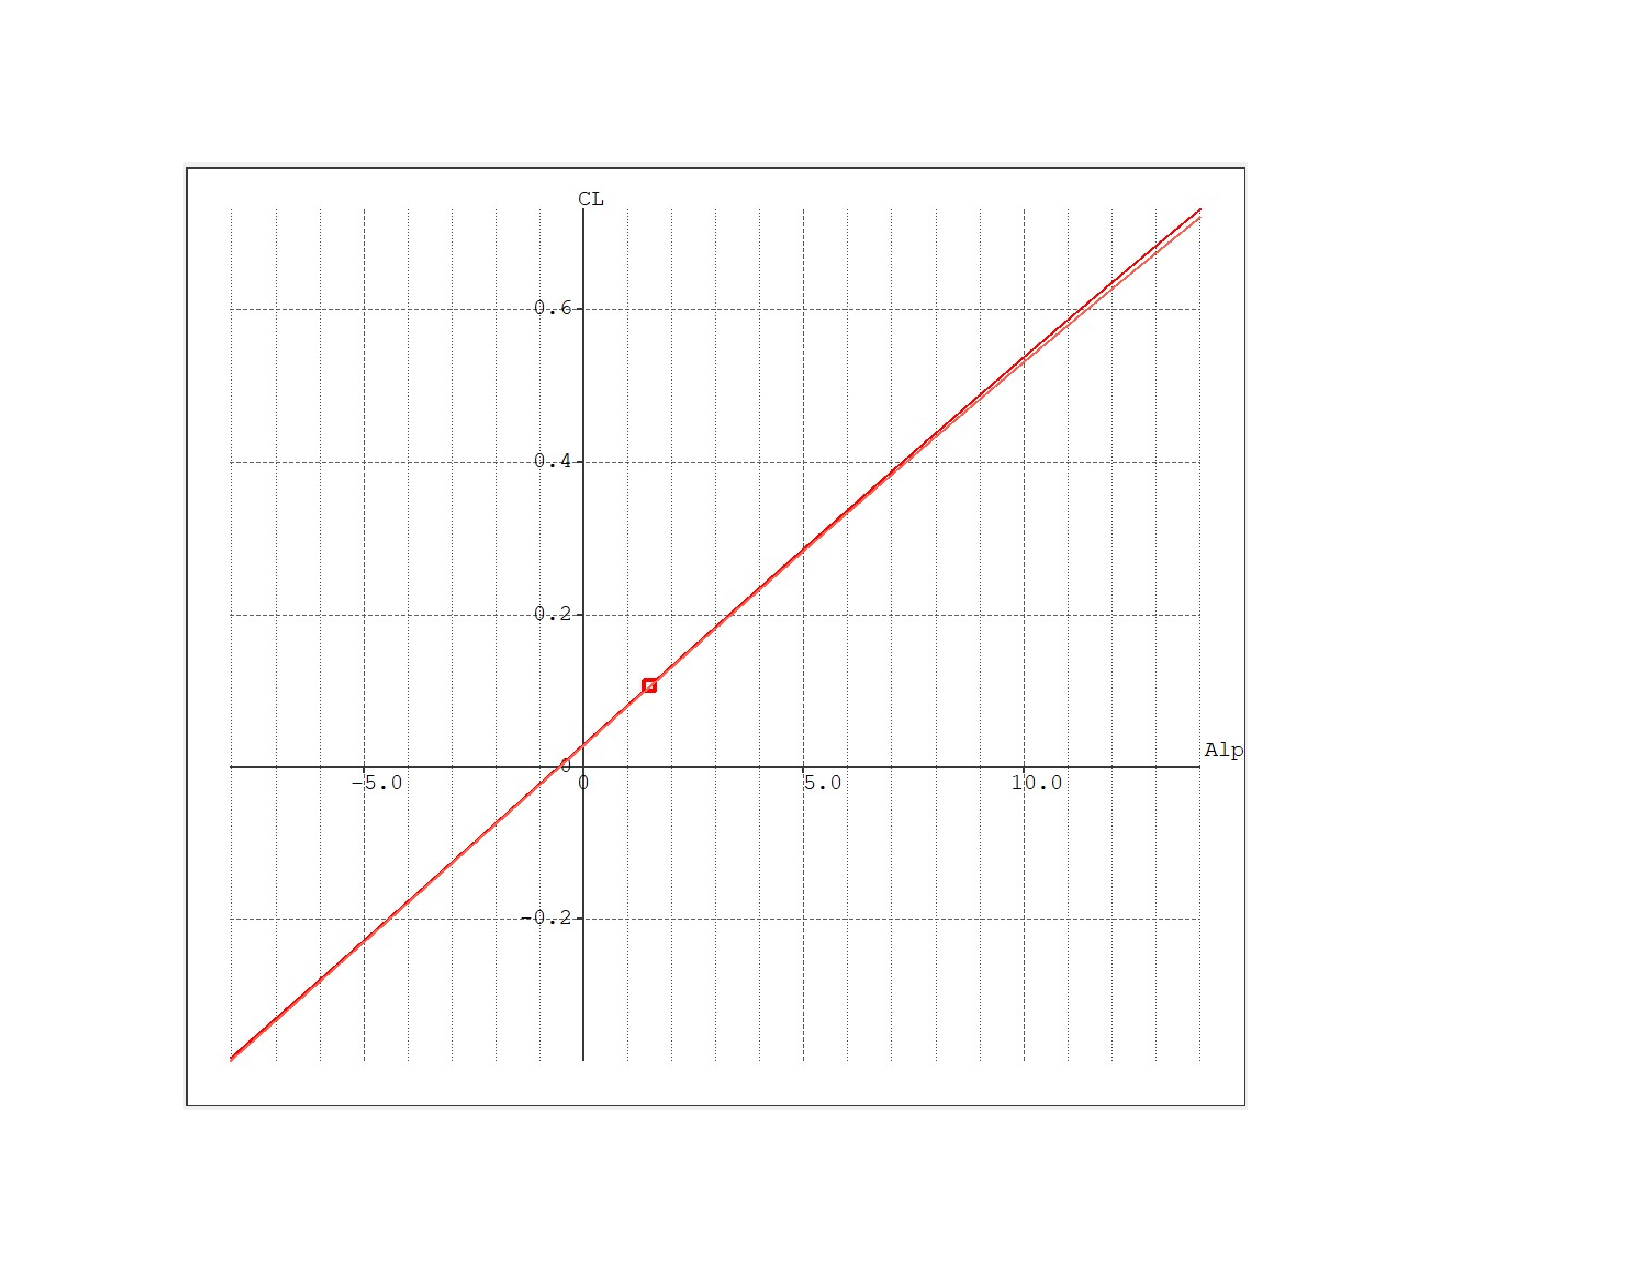
\includegraphics[scale=0.75]{Capitulo3/figs/CL ehekatl (1).pdf}
    \caption{EHEKATL BWB - Coeficiente de levantamiento}
    \label{Coeficiente de sustentación (levantamiento) respecto al ángulo de ataque de EHEKATL BWB}
\end{figure}
El coeficiente de levantamiento es un parámetro adimensional que describe la capacidad de un perfil o una aeronave para generar sustentación. 
El coeficiente de levantamiento se define como la relación entre la fuerza de sustentación (L), el área de referencia (S) de la superficie sustentadora, la densidad ($\rho$) y la la velocidad del flujo del aire (V) alrededor del cuerpo,
\begin{equation}
    C_L = \frac{L}{\frac{1}{2} \rho V^2 S}
\end{equation}
en la Figura \ref{Coeficiente de sustentación (levantamiento) respecto al ángulo de ataque de EHEKATL BWB} tenemos el coeficiente de sustentación de EHEKATL  BWB para las 4 velocidades propuestas en la Tabla \ref{tab: Re y velocidades} y su relación gráfica con tipo de línea en la Figura \ref{Tipo de línea de acuerdo con la técnica de simulación y la velocidad}. Todas las velocidades se simularon con ambos métodos, VLM1 y VLM2.
En la Figura \ref{Coeficiente de sustentación (levantamiento) respecto al ángulo de ataque de EHEKATL BWB} se perciben principalmente dos líneas, la línea que se encuentra con los valores por encima es de los resultados obtenidos corresponde con el método VLM1. Todas las velocidades dieron un coeficiente de levantamiento similar, por tanto, sólo se perciben dos líneas, las velocidades resueltas con el método VLM1 y VLM2. 

Si se considera la variación en el ángulo de ataque, tenemos el coeficiente de levantamiento en función del ángulo de ataque denotado $C_L(\alpha)$.  La relación entre el coeficiente de levantamiento y el ángulo de ataque se representa a menudo mediante una curva conocida como curva polar de sustentación
\begin{equation}
    C_L (\alpha) = a \alpha + C_{L0}
\end{equation}
dónde:
$a$ es la pendiente de la curva polar de sustentación, $\alpha$ es el ángulo de ataque y $C_{L0}$ es el coeficiente de levantamiento cuando el ángulo de ataque es cero. 
Es importante señalas que la función $C_L (\alpha)$ sólo considera la simplificación del modelo lineal, que es el resultado que obtuvimos con XFLR5 y considera un rango de $\alpha$ entre -8$^\circ$ a 14$^\circ$.  

En la Figura \ref{Coeficiente de arrastre de EHEKATL BWB} se tienen los resultados de simulación de EHEKATL BWB de acuerdo con el coeficiente de arrastre. 
\begin{figure}[!t]
    \centering
    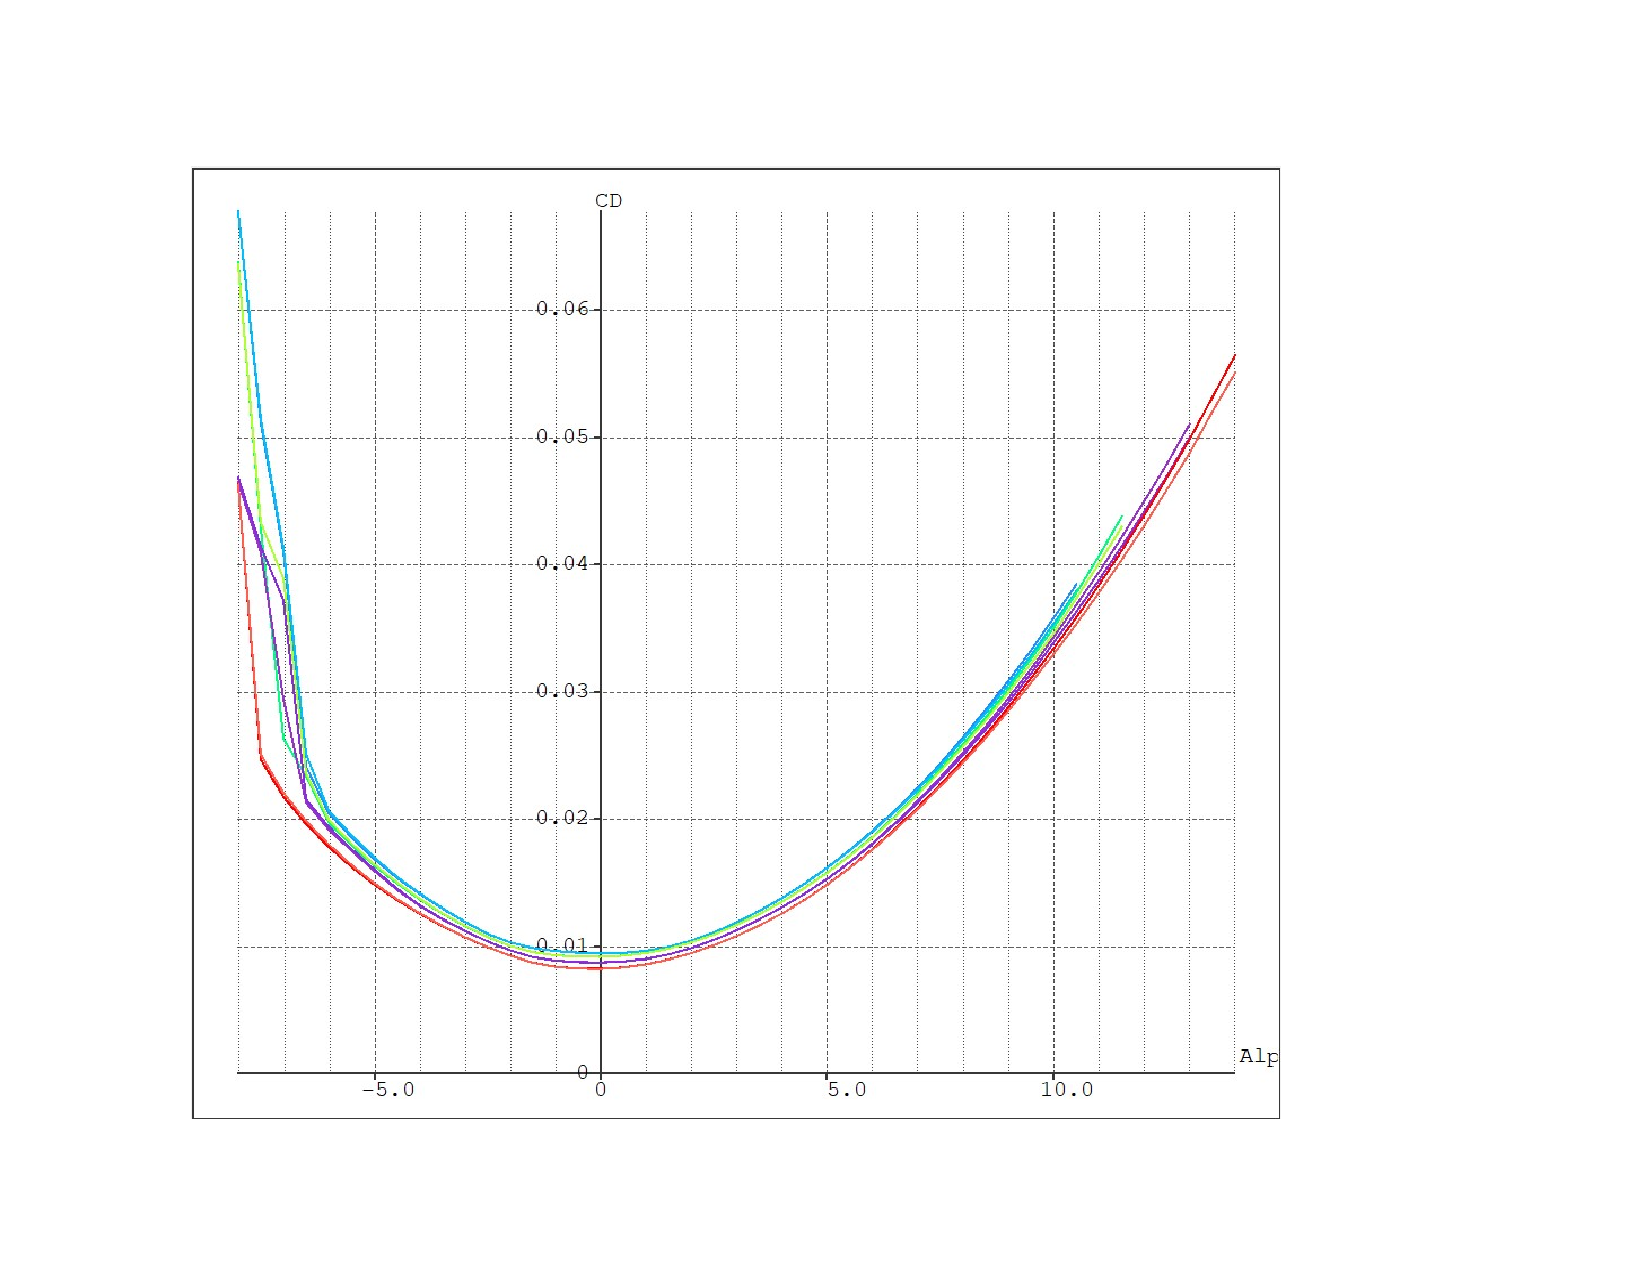
\includegraphics[scale=0.75]{Capitulo3/figs/arrastre ehekatl.pdf}
    \caption{EHEKATL BWB - Coeficiente de arrastre}
    \label{Coeficiente de arrastre de EHEKATL BWB}
\end{figure}
El coeficiente de arrastre es la cantidad de resistencia que enfrenta el cuerpo de la aeronave al moverse a través del fluido, el aire
\begin{equation}
    C_D = \frac{D}{\frac{1}{2} \rho V^2 S}
\end{equation}
dónde $D$ es la fuerza de resistencia o arrastre. Se compone de dos componentes principales: el coeficiente de arrastre viscoso $C_{D_0}$ y el coeficiente de arrastre inducido $C_{D_i}$. \footnote{En la sección de \textit{Superficie Alar y Potencia Requerida} desarrollamos exhaustivamente el cálculo del arrastre viscoso e inducido.}
\begin{equation}
    C_D = C_{D_0} + C_{D_i}
\end{equation}
\begin{figure}[!h]
    \centering
    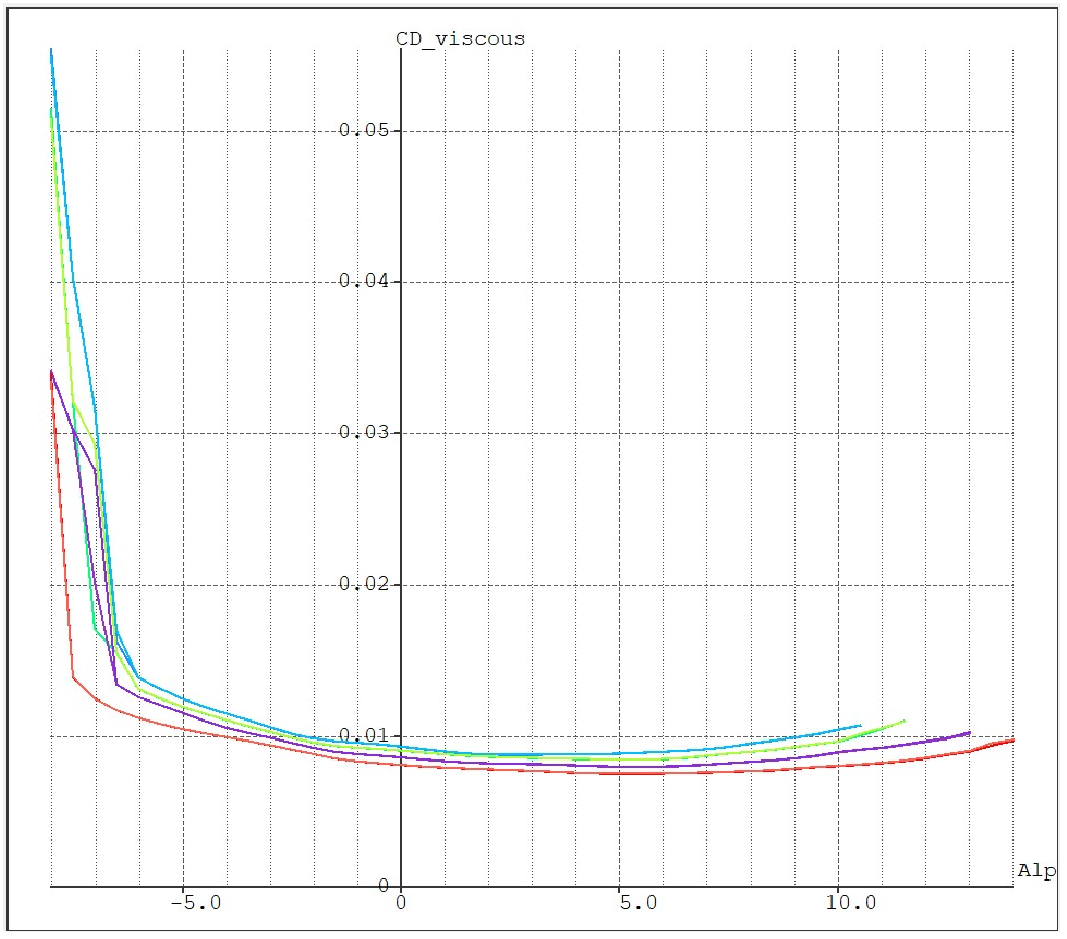
\includegraphics[scale=0.75]{Capitulo3/figs/arrastre viscoso ehekatl.pdf}
    \caption{EHEKALT BWB - Coeficiente de arrastre viscoso}
    \label{Coeficiente de arrastre viscoso}
\end{figure}
El coeficiente de arrastre viscoso está asociado con la fricción entre el cuerpo y el fluido que lo rodea. Depende de la forma del cuerpo y de la viscosidad del fluido. Para perfiles aerodinámicos, este componente tiende a disminuir a medida que aumenta el número de Reynolds. 
El coeficiente de arrastre inducido está asociado con la producción de vórtices y la generación de sustentación. Aumenta con el ángulo de ataque y con la eficiencia de la distribución de sustentación en la aeronave. 
El ángulo de ataque influye en ambos componentes del coeficiente de arrastre. 
\begin{figure}[!h]
    \centering
    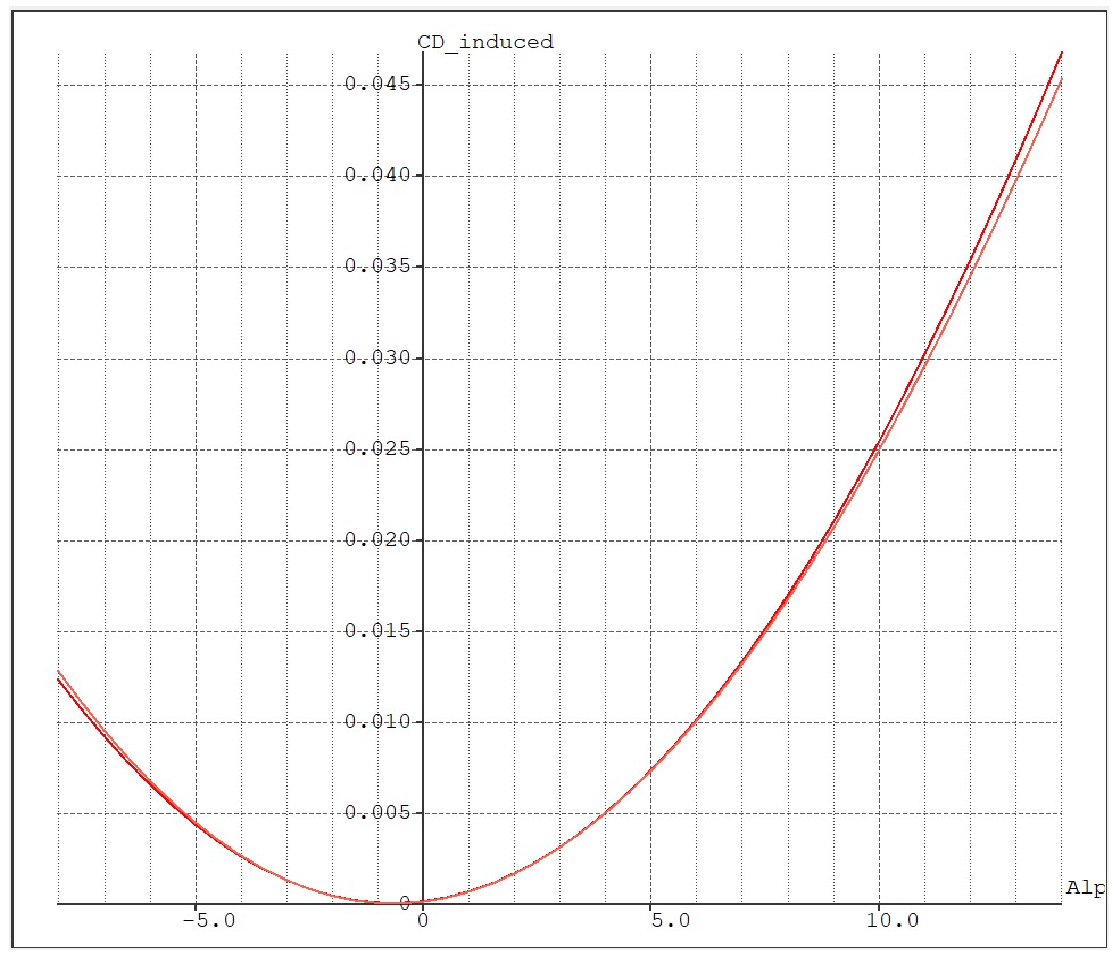
\includegraphics[scale=0.75]{Capitulo3/figs/arrastre inducido ehekatl.pdf}
    \caption{EHEKALT BWB - Coeficiente de arrastre inducido}
    \label{Coeficiente de arrastre inducido}
\end{figure}
A medida que aumenta el ángulo de ataque,  aumenta el coeficiente de arrastre total debido a un aumento en la sustentación y, por lo tanto, en el arrastre inducido. Sin embargo, el coeficiente de arrastre viscoso dada la geometría de EHEKATL BWB arroja un valor que desciende levemente para luego ascender, pero que dentro del rango de interés del ángulo de ataque podríamos considerar como constante. 

La razón de $C_L$ (coeficiente de sustentación) respecto a $C_D$ (coeficiente de arrastre) es una medida que proporciona información sobre la eficiencia aerodinámica de un objeto o una aeronave. Esta relación es conocida como la eficiencia aerodinámica o eficiencia en sustentación y es un indicador importante en el diseño de EHEKATL BWB y su desempeño.
En términos sencillos, representa cuánta sustentación se genera por cada unidad de arrastre producida.
Esta razón es especialmente importante en el diseño de aeronaves, ya que influye en aspectos como el alcance, la economía de combustible y la capacidad de carga de un avión.

La relación $C_L / C_D$ en función del ángulo de ataque es una representación gráfica que muestra cómo varía la eficiencia aerodinámica de una aeronave a medida que se cambia el ángulo de ataque.
En un gráfico se observan varias regiones de interés:

Region de Ascenso (Slope-Up Region):
En esta región,  $C_L$ aumenta a medida que se incrementa el ángulo de ataque, lo que significa que se está generando más sustentación. Sin embargo, el $C_D$ también aumenta, indicando un mayor arrastre. La eficiencia aerodinámica $C_L/C_D$ disminuye.

Punto de Sustentación Máxima (Max Lift Point):
Este es el punto en el gráfico donde la eficiencia aerodinámica $C_L/C_D$ es máxima. Representa el ángulo de ataque en el que la aeronave genera la máxima sustentación por unidad de arrastre.

Region de Descenso (Slope-Down Region):
Después del punto de sustentación máxima, si se sigue aumentando el ángulo de ataque, la eficiencia aerodinámica disminuye.  $C_L$ sigue aumentando, pero 
$C_D$ aumenta a un ritmo más rápido, lo que indica una pérdida de eficiencia.

La importancia de la relación $C_L/C_D/\alpha$:
El punto de sustentación máxima es crítico para el despegue y el aterrizaje de una aeronave, ya que indica el ángulo de ataque óptimo para generar la mayor sustentación con el menor arrastre posible.
La forma de la curva $C_L/C_D/\alpha$ también puede proporcionar información sobre la maniobrabilidad y el comportamiento de una aeronave en diferentes fases de vuelo.

\begin{figure}[!t]
    \centering
    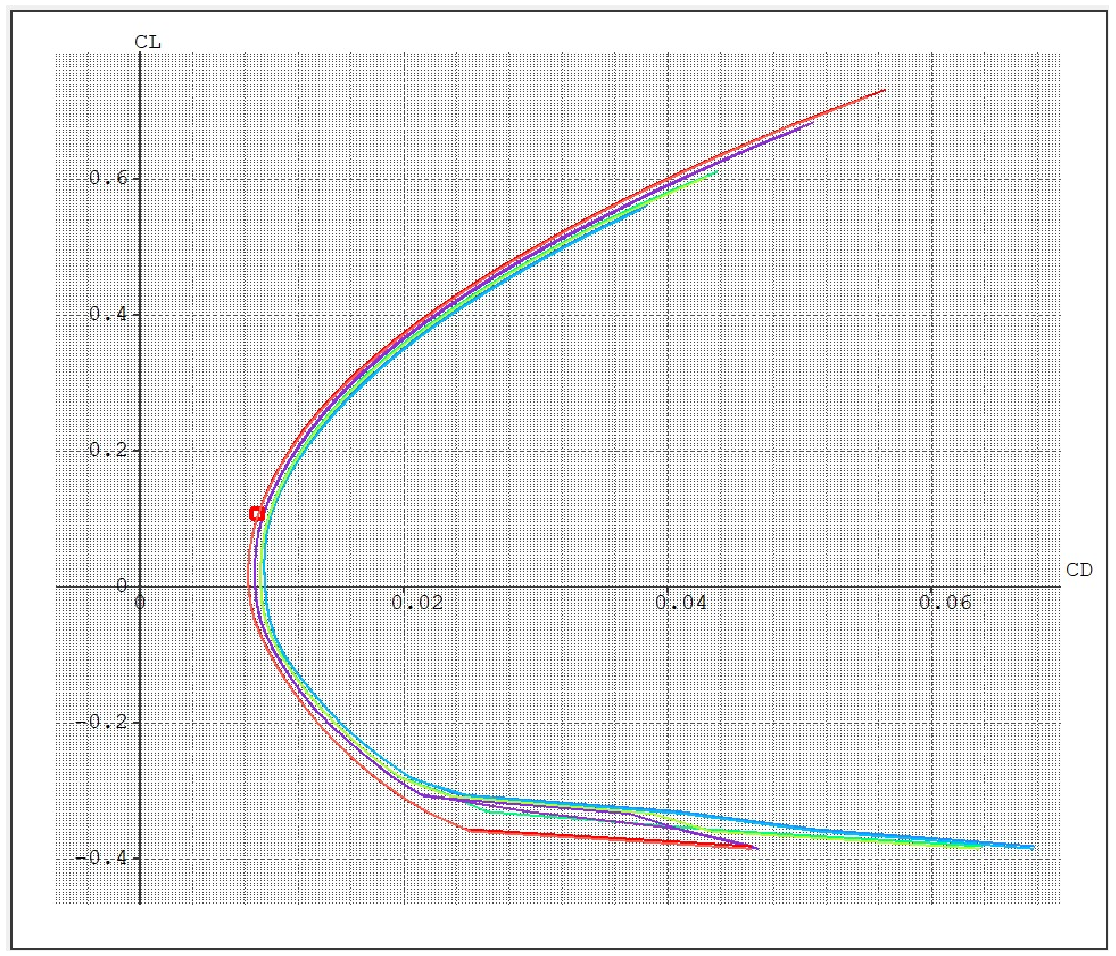
\includegraphics[scale=0.75]{Capitulo3/figs/cl y cd.pdf}
    \caption{EHEKALT BWB - razón polar coeficiente de sustentación / coeficiente de arrastre}
    \label{razón polar coeficiente de sustentación / coeficiente de arrastre}
\end{figure}

Los datos de este gráfico son fundamentales para los pilotos y diseñadores de aeronaves, ya que ayudan a determinar los perfiles de vuelo óptimos y las configuraciones de los controles para maximizar la eficiencia y el rendimiento de la aeronave.

Es importante destacar que cada aeronave tiene su propia curva $C_L/C_D/\alpha$ específica, y esta curva puede cambiar según la configuración (flaps, slats, etc.) y las condiciones de vuelo. Por lo tanto, se realizan pruebas y análisis detallados para determinar estas relaciones en condiciones reales. 
Para EHEKATL BWB y de acuerdo con las Figuras \ref{razón polar coeficiente de sustentación / coeficiente de arrastre} y \ref{EHEKALT BWB - Polar sustentacion arrastre ataque} se puede observar que la mayor eficiencia o mejor desempeño aerodinámico se da a altas velocidades. Si bien el coeficiente de sustentación mostró un comportamiento apenas incremental como función lineal, en el coeficiente de arrastre se mostró una diferencia que podemos considerar significativa y apreciable de manera visual, por tanto, la curva de la velocidad mayor simulada $35 m/s$ muestra el mejor desempeño en ambas funciones. 
La relación de incremento del coeficiente de sustentación respecto el coeficiente de arrastre comienza en 3 a 1 considerando un ángulo de ataque nulo, alrededor de 12 a 1 con un ángulo de ataque en equilibrio y una eficiencia máxima alrededor de 16 a 1 en las velocidades más bajas y 19 a 1 en las velocidades más altas, ver Figura \ref{EHEKALT BWB - Polar sustentacion arrastre ataque}. 
\begin{figure}[!t]
    \centering
    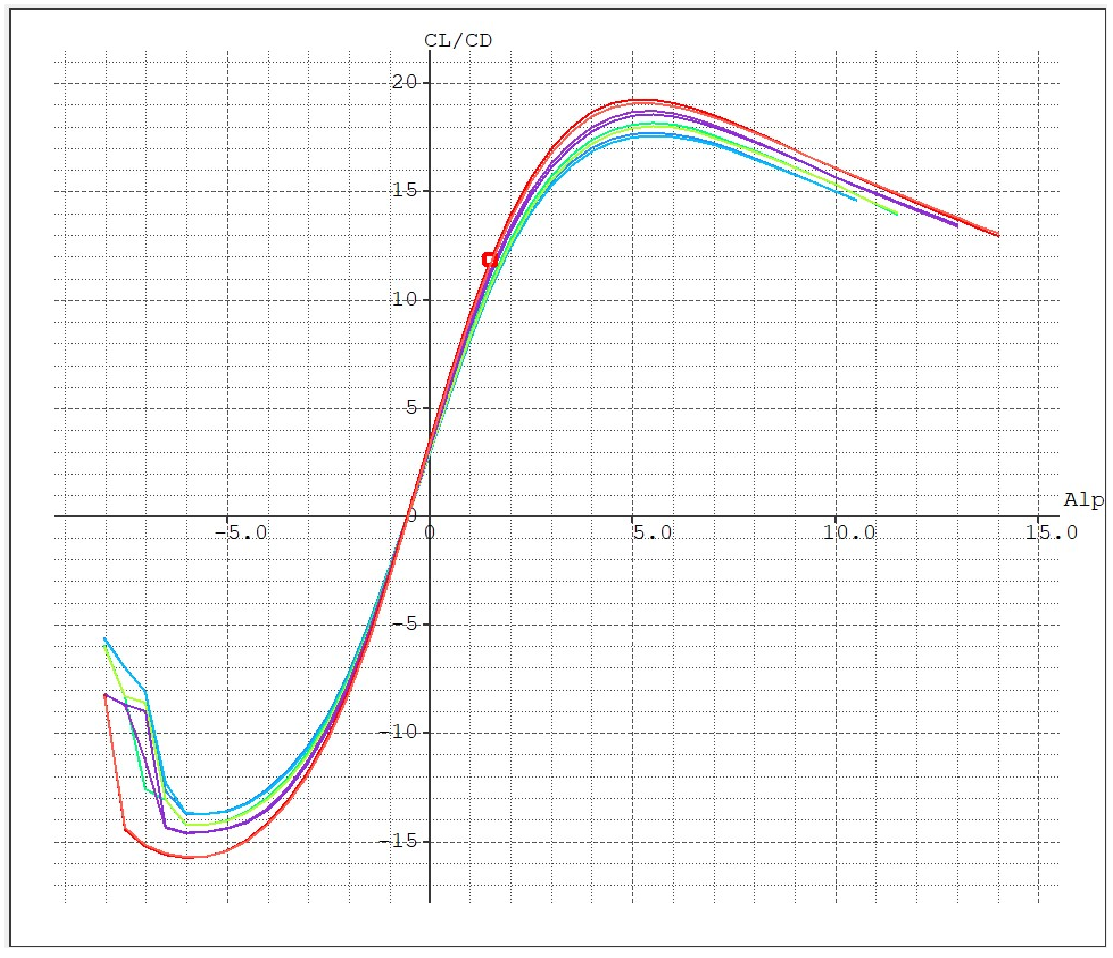
\includegraphics[scale=0.75]{Capitulo3/figs/cl cd.pdf}
    \caption{EHEKALT BWB - Polar sustentación/arrastre respecto al ángulo de ataque}
    \label{EHEKALT BWB - Polar sustentacion arrastre ataque}
\end{figure}

\medskip

%%%%%%%%%%%%%%%%%%%%%%%%%%%%%%%%%%
\subsection{Análisis de Estabilidad con XFLR5}
En un vuelo normal es usual para los pilotos ajustar los controles de la aeronave tal que liberando los controles la aeronave continua su vuelo en la condición de vuelo deseada. 
En inglés se dice que la aeronave fue \textit{trimmed}, y \textit{trim} define la condición inicial dónde las variables de interés pueden ser estudiadas. 
El objetivo de \textit{trimming} es llevar las fuerzas y los momentos que actúan en la aeronave a un estado en equilibrio.
Esta condición se cumple cuando las fuerzas axiales, normales y laterales; como los momentos de alabeo, cabaceo y guiñada son todos cero. 
El balance de fuerzas y momentos es expresado en los requerimientos como levantamiento igual a peso $L=W$ y empuje igual a arrastre $D=T$, esto provee la estabilidad en el estado de equilibrio incluso después de una perturbación generada por las entradas de control dirigidas por el piloto o autopiloto, o por influencias externas como perturbaciones. 
\begin{figure}[!h]
\centering
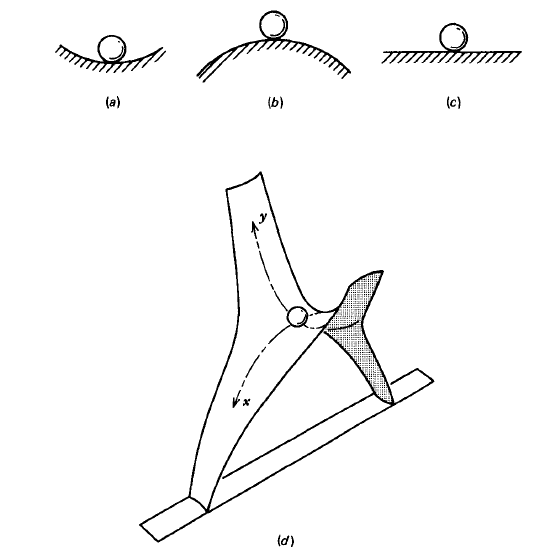
\includegraphics[scale=0.90]{Capitulo3/figs/4 22.png}
\caption{Bola en equilibrio, estable e inestable \cite{Etkin1996}}
\label{fig: Bola en equilibrio, estable e inestable}
\end{figure}
Para mantener un estado de equilibrio se requiere el ajuste simultaneo de las principales variables de vuelo en los seis grados de libertad de la aeronave que dependen del número de Mach, el ángulo de la trayectoria de vuelo, la configuración geométrica de la aeronave, el peso y la posición del centro de gravedad. 
%
Con parámetros variantes en el tiempo tenemos que ajustar el equilibrio durante el vuelo tanto como sea necesario. 
%
La simetría típica de las aeronaves confiere propiedades aerodinámicas que usualmente reducen la tarea al ajuste longitudinal únicamente. 
El ajuste para el equilibrio lateral-direccional es necesario cuando se pierde esta simetría aerodinámica, que puede ocurrir cuando un motor en una aeronave multi-motor deja de funcionar, por ejemplo. 
%
Un cuerpo se encuentra en equilibrio si esta en reposo o en movimiento uniforme, es decir, si tiene momentos lineales y angulares constantes. 
%
En otras palabras, el equilibrio de una aeronave en movimiento uniforme carece de rotación, esto es, un movimiento rectilíneo de traslación, dado que las fuerzas aerodinámicas son dependientes del ángulo de orientación de la aeronave respecto a la trayectoria de vuelo, y porque el resultante de estas fuerzas debe balancear con exactitud de acuerdo al peso y centro de gravedad de la aeronave. 
%
La estabilidad o la falta de ella, es una propiedad de los estados en equilibrio. 
%
Hablamos de un estado de equilibrio estable cuando el cuerpo (aeronave) es ligeramente perturbada en cualquiera de sus grados de libertad, y de inmediato regresa a su estado de equilibrio inicial, \cite{Etkin1996}. 

Se utiliza la Figura \ref{fig: Bola en equilibrio, estable e inestable} para explicar el equilibrio neutral e inestable. 
%
La bola que se encuentra en el centro de la geometría (d) es estable respecto a la dirección $y$, pero inestable si desplaza en $x$. 
Las aeronaves cumplen este principio, dado que pueden ser estables con respecto a un grado de libertad, pero inestable con respecto a otro. 
%
Dos tipos de inestabilidad son relevantes en la dinámica de una aeronave:
La \textbf{inestabilidad estática} continuamente separa a la aeronave de su condición de equilibrio, un ejemplo es bola en (b).
La \textbf{inestabilidad dinámica} es un fenómeno complicado dónde la aeronave oscila alrededor del estado de equilibrio con un incremento constante en su amplitud (no explicable con la figura \ref{fig: Bola en equilibrio, estable e inestable}).
%
Cuando aplicamos el concepto de estabilidad a la aeronave, dos clases deben ser consideradas: 
La \textbf{estabilidad inherente} es una propiedad básica de la geometría de la aeronave con sus controles fijos o libres.
La \textbf{estabilidad sintética} es la que provee un Sistema de Control de Vuelo Automático (AFCS) y desaparece si falla el sistema de control. 
%
Los AFCS son capaces de estabilizar aeronaves inherentemente inestables, como el caso de las aeronaves de ala-integrada. También mejoran su estabilidad, a este último se le conoce como \textbf{Sistema Aumentado de Estabilidad (SAS)}. El caso de una aeronave de ala-integrada con SAS se mostró en antecedentes con la aeronave X-48 B/C de NASA. 
%
En un autopiloto el sistema a lazo cerrado debe estabilizar en respuesta las perturbaciones atmosféricas y comandos que vienen del sistema de navegación. 
%
Finalmente, los roles principales que desempeña un controlador de vuelo son los siguientes:
Fijar o cambiar la condición de equilibrio (velocidad o ángulo de ascenso). Un control adecuado debe ser capaz de producir un rango completo de los estados de equilibrio donde la aeronave pueda operar.
Producir movimientos acelerados, o no estados de no equilibrio, mientras se llevan a cabo maniobras.

En resumen, la estabilidad de una aeronave está dividida en estabilidad estática y estabilidad dinámica. 
%
Las características de la estabilidad estática determinan la \textit{trimmability} o ajuste hacia el equilibrio de la aeronave. 
La estabilidad estática es comúnmente interpretada para describir la tendencia de convergencia dada una condición inicial de equilibrio seguida de una pequeña perturbación hacia esta condición de equilibrio.
%
La estabilidad dinámica describe el movimiento de transición en el proceso de recuperar el equilibrio después de una perturbación. 
%
Para desarrollar el análisis de estabilidad de EHEKATL BWB vamos a tomar los resultados obtenidos en la simulación con XFLR5. 

\medskip
%%%%%%%%%%%%%%%%%%%%%%%%%%%%%%%%%%%%%%%%%%%%%%%%%%%%%%%%%%%%%%%%%%%%%%%%%
\textbf{Estabilidad estática de EHEKATL BWB}

La estabilidad estática puede ser explicada con la Figura \ref{fig: Bola en equilibrio, estable e inestable}. 
La bola en (b) es \textbf{estáticamente inestable} dado que después de que las fuerzas y momentos actúan sobre el cuerpo resulta una perturbación que el cuerpo no puede recuperar, y se aleja continuamente de su estado de equilibrio. 
La figura (a) es \textbf{estáticamente estable} dado que después de que las fuerzas y momentos actúan en el cuerpo éste tiende a recuperar su estado de equilibrio inmediatamente. 
La figura (c) es \textbf{neutralmente estable} si el cuerpo es perturbado pero el momento se mantiene en cero y el cuerpo se mantiene en equilibrio. 
%
En la dinámica de vuelo la estabilidad e inestabilidad son muy importantes. Es muy raro que la estabilidad neutral ocurra en la dinámica de vuelo de vehículos aéreos. 

\medskip

%%%%%%%%%%%%%%%%%%%%%%%%%%%%%%%%%%%%%%%%%%%%%%%%%%%%%%%%%%%%%%%%%%%%%%%%%
\textbf{Estabilidad estática longitudinal}

La estabilidad estática longitudinal refiere a la estabilidad de la aeronave en el plano simétrico x-z y respecto al momento de cabeceo.
Si una aeronave es longitudinalmente estable un pequeño incremento en el ángulo de ataque causará un cambio en el momento de cabeceo que decrecerá el ángulo de ataque. En el caso contrario, si hay un pequeño decrecimiento en el ángulo de ataque entonces se generará un cambio en el momento de cabeceo que incrementará el ángulo de ataque, \cite{Neubacher2008}.

La siguiente ecuación muestra la relación del momento de cabeceo dada una aeronave sin empenaje (tailless aircraft), en un vuelo en equilibrio cuasi-estable, con masa constante y para ángulos de ataques pequeños. 
\begin{equation}
    C_m = C_{m0} - C_L (x_{cg} - x_{ac})
\end{equation}
El momento de cabeceo está en función del coeficiente de levantamiento $C_L$, la diferencia de la distancia del centro de gravedad al centro aerodinámico $(x_{cg}-x_{ac})$ y el coeficiente de momento generado por las características del ala $C_{m0}$. 
%
De las restricciones más importantes en la estabilidad estática longitudinal es que $M_w, M_q$ deben ser negativos, de otra manera, tendríamos inestabilidad estática longitudinal, \cite{Neubacher2008}. 
%
Entonces, los criterios para asegurar la estabilidad estática longitudinal serían los siguientes:
\begin{itemize}
    \item Pendiente negativa en la función del momento de cabeceo $C_m$ respecto al ángulo de ataque $\alpha$
    \item Valores negativos en los coeficientes de momento de cabeceo respecto a la velocidad normal y tasa de cabeceo $M_w, M_q$ 
    \item Valores negativos en los coeficientes de fuerza axial respecto a la velocidad axial y fuerza normal respecto a la velocidad normal $X_u, Z_w$
\end{itemize}
\begin{figure}[t]
    \centering
    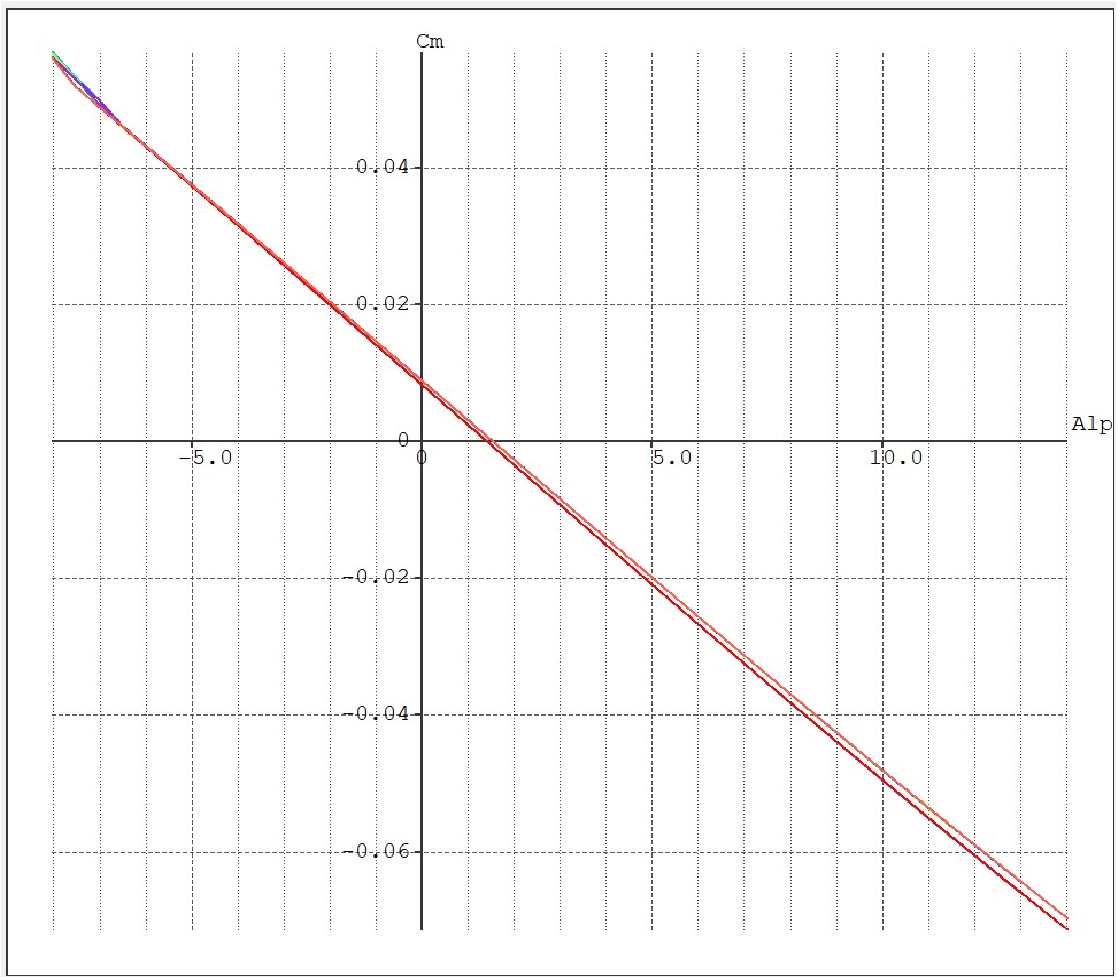
\includegraphics[scale = 0.65]{Capitulo3/figs/Cm a.pdf}
    \caption{Estabilidad estática en la dinámica longitudinal}
    \label{Estabilidad estática en la dinámica longitudinal}
\end{figure}

Dados los resultados de simulación de la Figura \ref{Estabilidad estática en la dinámica longitudinal} se cumple el criterio de pendiente negativa para el $C_m$ respecto $\alpha$, garantizando la estabilidad estática longitudinal.
Los criterios de valores negativos para $M_w$,$M_q$ y $X_u$,$Z_w$ también se cumplen. Estos valores pueden validarse en el capítulo de diseño de controladores en la Tabla \ref{Coeficientes dimensionales longitudinales de EHEKATL BWB} y también en la Tabla \ref{Coeficientes dimensionales longitudinales de EHEKATL BWB adaptive}, dónde son empleados para las simulaciones de prueba de control longitudinal de EHEKATL BWB con PYTHON. 

\begin{figure}[!t]
    \centering
    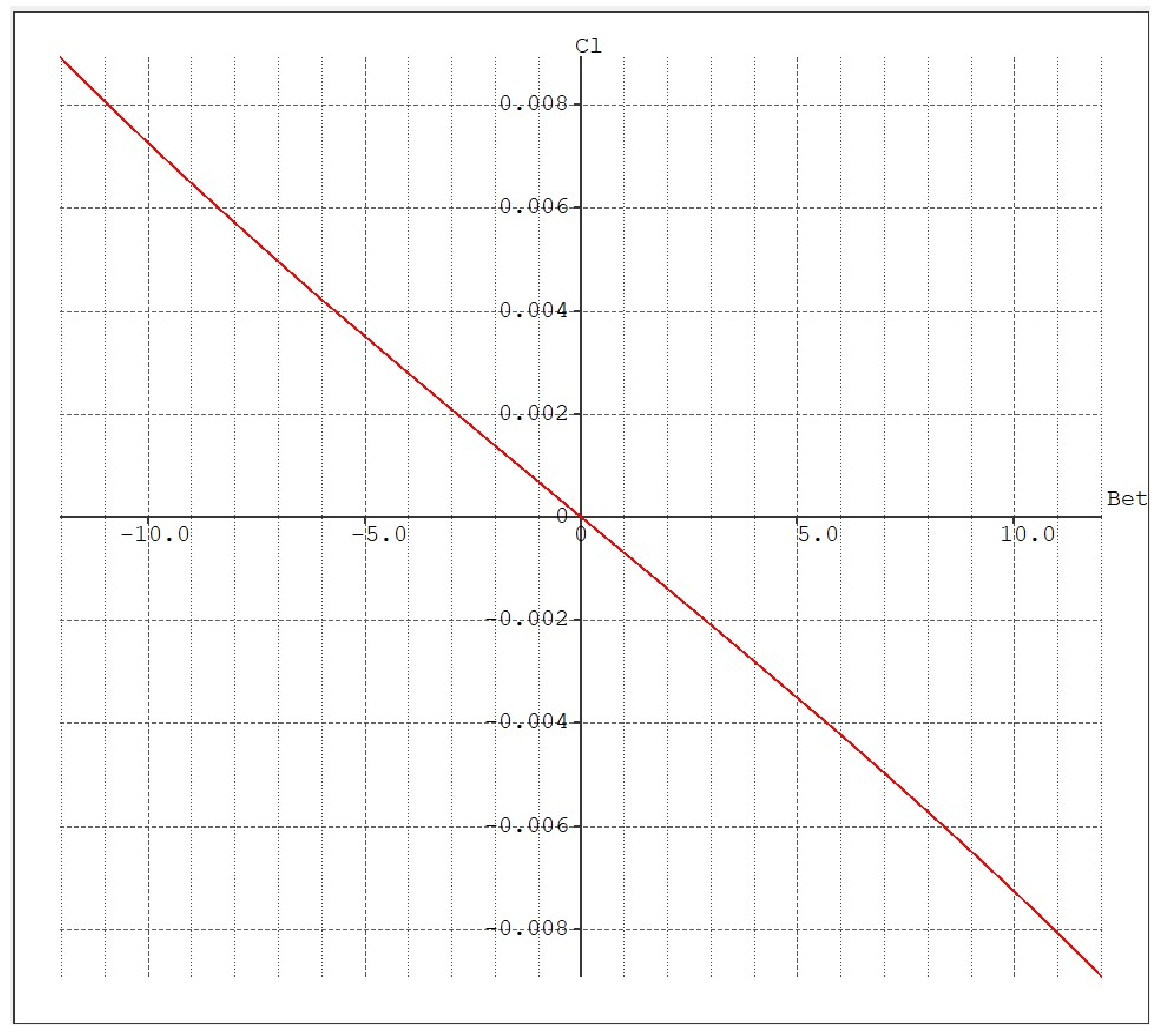
\includegraphics[scale = 0.66]{Capitulo3/figs/cl beta (2).pdf}
    \caption{Estabilidad estática lateral}
    \label{Estabilidad estática lateral}
\end{figure}


Todas las simulaciones de estabilidad muestran las velocidades empleadas en la Tabla \ref{tab: Re y velocidades} y su color representativo respectivo. 
Las velocidades se agrupan en dos funciones de acuerdo al tipo de simulación VLM1 y VLM2. La pendiente ligeramente más pronunciada es de VLM2. El rango de $\alpha$ para el momento de cabeceo en equilibrio se encuentra entre 1.45$^\circ$ y 1.55$^\circ$. 
Cuando el momento de cabeceo es cero es fundamental conocer el ángulo de ataque, dado que en este punto se pueden liberar los controles asegurando un vuelo recto y nivelado.
Se toma la media de $\alpha$ en 1.5$^\circ$ como valor específico para cálculos posteriores.
%
Partiendo del punto de equilibrio (valor de $\alpha$ que hace cero a $C_m$, en este caso $\alpha$ de  1.5$^\circ$) se observa que si el ángulo de ataque disminuye se genera un momento positivo, y si el ángulo de ataque aumenta se genera un momento negativo. En un sentido físico, si la aeronave se encuentra en un vuelo recto y nivelado ($\alpha_e$ con $C_m = 0$) y una perturbación disminuye o aumenta el ángulo de ataque, la aeronave tiene la capacidad de recuperar la condición de equilibrio después de la perturbación. 

\begin{figure}[!t]
    \centering
    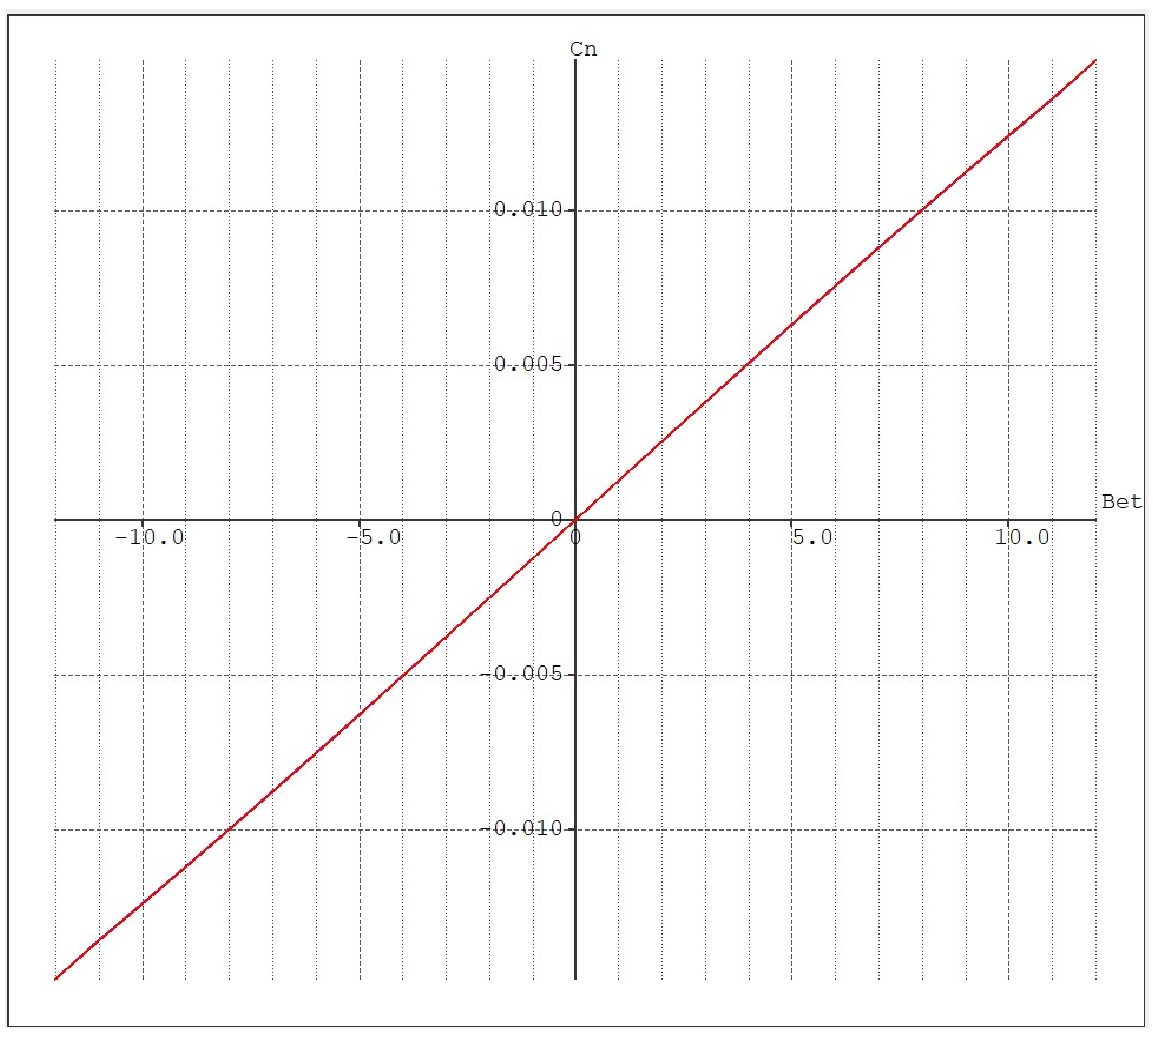
\includegraphics[scale = 0.65]{Capitulo3/figs/Cn beta (1).pdf}
    \caption{Estabilidad estática direccional}
    \label{Estabilidad estática direccional}
\end{figure}


\medskip
%%%%%%%%%%%%%%%%%%%%%%%%%%%%%%%%%%%%%%%%%%%%%%%%%%%%%%%%%%%%%%%%%%%%%%%%
\textbf{Estabilidad estática lateral-direccional}

De acuerdo con \cite{Neubacher2008}, la estabilidad estática lateral concierne con la habilidad de la aeronave para mantener un equilibrio a nivel del ala en el sentido de la acción de alabeo. 
%
El parámetro con la mayor influencia en la estabilidad estática lateral es el ángulo diedro del ala. 
%
El efecto del diedro en configuraciones de aeronaves sin empenaje es igual a su implementación en aeronaves convencionales con empenaje. 
%
A través de la configuración de este parámetro (diedro) podemos diseñar y ajustar la estabilidad estática lateral de acuerdo con el nivel de aceptabilidad que estemos buscando. 

Para garantizar la estabilidad estática lateral después de una perturbación en el momento de alabeo se establecen los siguientes criterios:
\begin{itemize}
    \item Pendiente negativa en la función del momento de alabeo $C_l$ respecto el ángulo de derrape $\beta$
    \item El valor del momento de alabeo respecto al ángulo de derrape $L_\beta$ debe ser negativo
    \item  El valor del momento de alabeo respecto a la velocidad angular de alabeo $L_p$ deber ser negativo
    \item El valor del coeficiente de fuerza lateral respecto al ángulo de derrape $Y_{\beta}$ debe ser negativo
\end{itemize}

La estabilidad estática direccional trata la estabilidad de la aeronave en el eje $z$.
Se busca que la aeronave pueda regresar a la condición de equilibrio después de experimentar una perturbación en el momento de guiñada.
Para asegurar que la aeronave recobre la estabilidad debemos de cumplir el siguiente criterio:
\begin{itemize}
    \item Pendiente positiva en el momento de guiñada $C_n$ respecto al ángulo de derrape $\beta$
    \item El valor del coeficiente de momento de guiñada respecto al ángulo de derrape $N_\beta$ debe ser positivo
\end{itemize}

De acuerdo con los resultados de simulación de la Figuras \ref{Estabilidad estática lateral} y \ref{Estabilidad estática direccional} se cumple el criterio de estabilidad estática con pendiente negativa en $C_l$ respecto a $\beta$ para la estabilidad lateral y pendiente positiva en $C_n$ respecto a $\beta$ para la estabilidad direccional. 
De igual manera, se cumplen los criterios de valores negativos en los coeficientes $L_\beta$,$L_p$,$Y_{\beta}$ para la estabilidad lateral y el valor positivo en el coeficiente $N_\beta$ para la estabilidad direccional. Tales valores se pueden validar en el capítulo de diseño de controladores en la Tabla \ref{Coeficientes dimensionales laterales de EHEKATL BWB}, dónde se emplearon para realizar las simulaciones de control lateral-direccional de EHEKATL BWB en PYTHON. 

%%%%%%%%%%%%%%%%%%%%%%%%%%%%%%%%%%%%%%%%%%%%%%%%%%%%%%%
\section{Diseño de EHEKATL BWB en Plane Maker}


Plane Maker es un programa utilizado en el desarrollo del simulador de vuelo X-PLANE. Es conocido por su realismo en la dinámica de vuelo y es utilizado por profesionales de la aviación, aficionados y entusiastas del vuelo para entrenamiento e investigación.
Plane Maker es una interfaz gráfica de usuario (GUI) que permite a los usuarios crear y modificar modelos de aeronaves dentro del entorno de X-PLANE. Proporciona una plataforma para diseñar y personalizar varios aspectos de una aeronave, incluida su geometría, aerodinámica, peso y equilibrio, sistemas y características de rendimiento.

Para el diseño geométrico de EHEKATL BWB se configuraron un total de 20 secciones alares, incluyendo aletas y estabilizadores verticales, ver Figura \ref{Diseño Aerodinámico de EHEKATL BWB en Plane Maker}. La secciones fueron numeradas en el mismo orden que Plane Maker, y corresponden con el diseño previo en XFLR5. 
La parametrización en Plane Maker es particular. En el bloque que se muestra debajo del diseño geométrico de EHEKATL BWB en la Figura \ref{Diseño Aerodinámico de EHEKATL BWB en Plane Maker} se aprecia la parametrización o especificaciones de la sección alar número uno (1), que corresponde al semi-ala izquierda en la sección central del cuerpo de EHEKATL BWB. Utilizando esta sección número uno a manera de ejemplo, el primer parámetro es la distancia desde el perfil raíz (adjunto al no. 11) al perfil punta (ajunto al no. 2) llamado \textit{semi-length} o semi-ala. Esta distancia no se considera como en XFLR5, dónde es una distancia lineal (en el eje $y$) y fácil de parametrizar respecto a la envargudura. En Plane Maker está distancia se considera desde el 25$\%$ (partiendo del borde de ataque) de cada perfil, desde el perfil raíz y hacia el perfil de punta. Para poder trabajar este nuevo diseño de acuerdo con los requerimientos de Plane Maker se desarrollo un código en PYTHON que extrapola las parametrizaciones del diseño de EHEKATL BWB en XFLR5 para adaptarlo a los campos de Plane Maker considerando el cambio de unidades del sistema internacional al sistema inglés. Tal código puede revisarse en la cuenta de GitHub del autor de la tesis. El link se encuentra en la sección de apéndices \ref{a codigos python}. 
Posteriormente, en el mismo bloque de la Figura \ref{Diseño Aerodinámico de EHEKATL BWB en Plane Maker} se tiene el ajuste para la cuerda del perfil raíz (\textit{root chord}) y la cuerda del perfil punta (\textit{tip chord}). 
Después, en la parte central de este mismo bloque se ajustan el ángulo de flechado y el ángulo de diedro, así como la sección de la semi-ala que se esta diseñando, izquierda o derecha. Finalmente, se ajustan las coordenadas de la sección de la semi-ala en los tres ejes: \textit{long arm} para la distancia en $x$, \textit{lat arm} para la distancia en $y$ y \textit{vert arm} para la distancia en $z$.  
Las secciones de la semi-ala izquierda ala 2 y 4, y de la semi-ala derecha 12 y 14 se respetaron de acuerdo con el diseño previo en XFLR5. En XFLR5 se diseñaron estas secciones para poder diseñar las ACS con la geometría establecida en el borde de fuga. Se respetaron el diseño de EHEKATL BWB en Plane Maker para tener exactamente el mismo modelo propuesto en las secciones anteriores. 

\begin{figure}[!t]
    \centering
    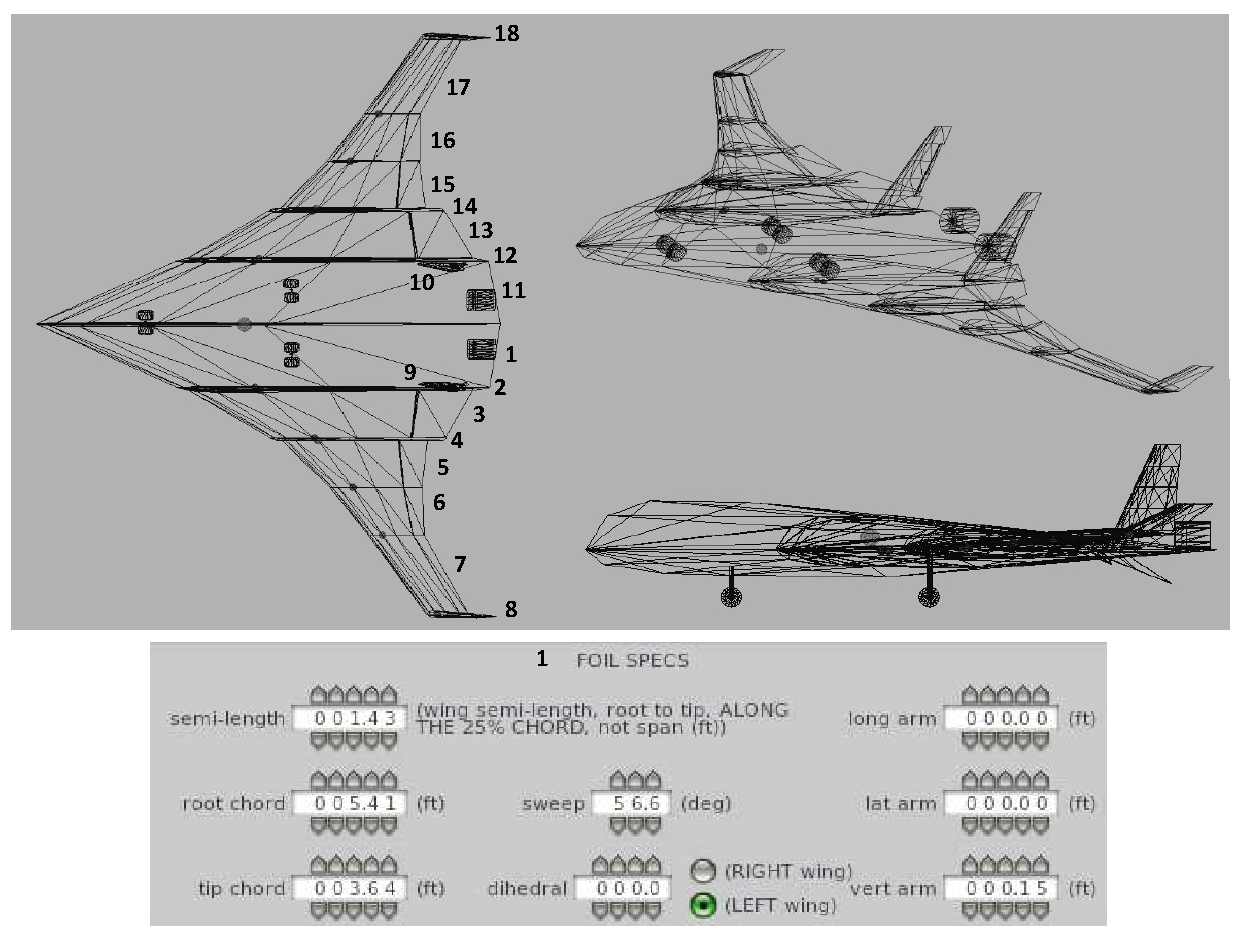
\includegraphics[scale=0.62]{Capitulo3/figs/Diseño EHEKATL BWB Plane Maker 2 (1).pdf}
    \caption{Diseño de la aeronave EHEKATL BWB en Plane Maker}
    \label{Diseño Aerodinámico de EHEKATL BWB en Plane Maker}
\end{figure}

La configuración de las superficies de control aerodinámicas de EHEKATL BWB se encuentran en la Figura \ref{Dimensión de las ACS de EHEKATL BWB}.
Las ACS se dimensionaron de la misma manera que en XFLR5.
En la Figura \ref{Dimensión de las ACS de EHEKATL BWB} se aprecian dos primeras columnas (de izquierda a derecha) dónde viene el nombre de la ACS a dimensionar y la leyenda \textit{chord ratio} que alude al porcentaje de cuerda que se considera para la superficie de control, desde el borde de fuga hacia el borde de ataque. La primer columna es para el porcentaje respecto a la cuerda raíz, y la segunda respecto a la cuerda de punta. 
\textbf{EHEKATL BWB cuenta con dos pares de elevadores, dos pares de alerones y un par de timones de dirección}. Cuando se observa la leyenda \textit{aileron 1} corresponde, por ejemplo, al par de alerones localizados en la sección de la semi-ala izquierda no. 7 y la sección de la semi-ala derecha no. 17. Este mismo principio aplica para elevadores pero no así para timones de dirección, dónde si refiere a cada elemento y no su par. 
Todas las ACS se dimensionaron a un 20$\%$ tanto del perfil raíz como del perfil punta.Asimismo, La deflexión de todas las ACS se establece en $-30/+30$. Esta parametrización se aprecia en las siguientes dos columnas de la Figura \ref{Dimensión de las ACS de EHEKATL BWB}, dónde la primera corresponde a a deflexión hacia abajo y la segunda la deflexión hacia arriba. 
Por último, se configuraron las ACS como \textit{Smooth with no gaps}, que se traduce como suave y sin brechas, o liso sin espacios. Esta parametrización permite apreciar le borde de fuga como única geometría si ninguna ACS tiene deflexión. 

\begin{figure}[!t]
    \centering
    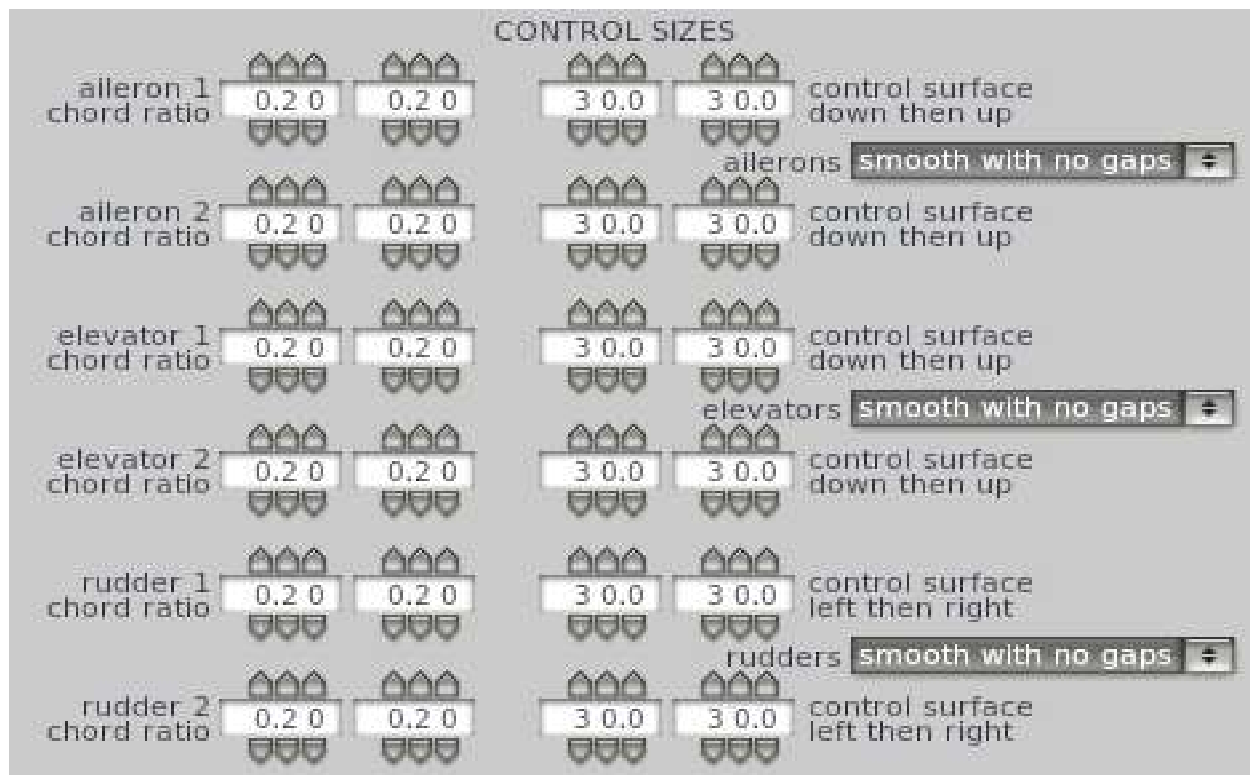
\includegraphics[scale=0.5]{Capitulo3/figs/ACS plane maker.pdf}
    \caption{Dimensión de las ACS de EHEKATL BWB en Plane Maker}
    \label{Dimensión de las ACS de EHEKATL BWB}
\end{figure}

Una vez definido el diseño geométrico y las ACS de la aeronave EHEKATL BWB en Plane Maker, deben implementarse los perfiles MH78 y MH80 diseñados en Airfoil Maker, además del NACA 0009 que ya se encuentra en el programa.
El perfil MH80 se implementa en la sección central dónde se localiza la carga útil y los distintos componentes de aviónica y se limita hasta dónde se termina la sección con la primer ACS, o elevadores principales. El resto del ala es perfil MH78 salvo la aleta que es NACA 0009 junto con los estabilizadores verticales. 
En la Figura \ref{Implementación de perfiles de EHEKATL BWB} se observa la implementación de los perfiles en la semi-ala derecha y estabilizadores verticales. Además, se establece el perfil Clark-Y para las hélices o propelas de los motores. 
%
\begin{figure}[!t]
    \centering
    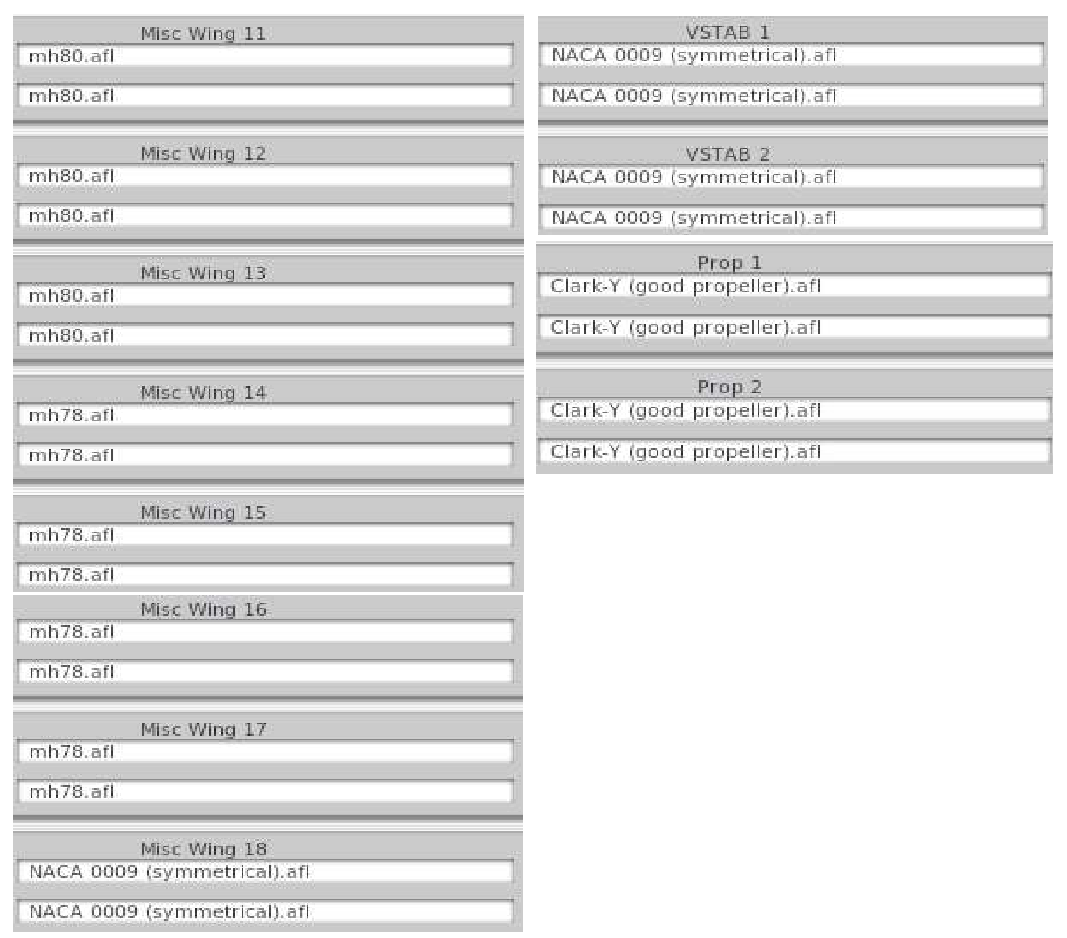
\includegraphics[scale=0.7]{Capitulo3/figs/perfiles plane maker.pdf}
    \caption{Implementación de perfiles MH78,MH80 y NACA 0009 para EHEKATL BWB en Plane Maker}
    \label{Implementación de perfiles de EHEKATL BWB}
\end{figure}
%


En la Figura \ref{Especificaciones de motores} se muestra las especificaciones los motores. Dado que en X-PLANE los motores Jet consideran cámara de combustión, y entonces, una capacidad mayor de empuje para aplicaciones de aeronaves a escala real, los motores seleccionados para EHEKATL BWB son motores ductofan que constan de un fan dentro de un ducto energizado por baterías eléctricas. Los perfiles Clark-Y aplican en esta geometría de las hélices de los fan dentro de lo ductos. 
 
\begin{figure}[!t]
    \centering
    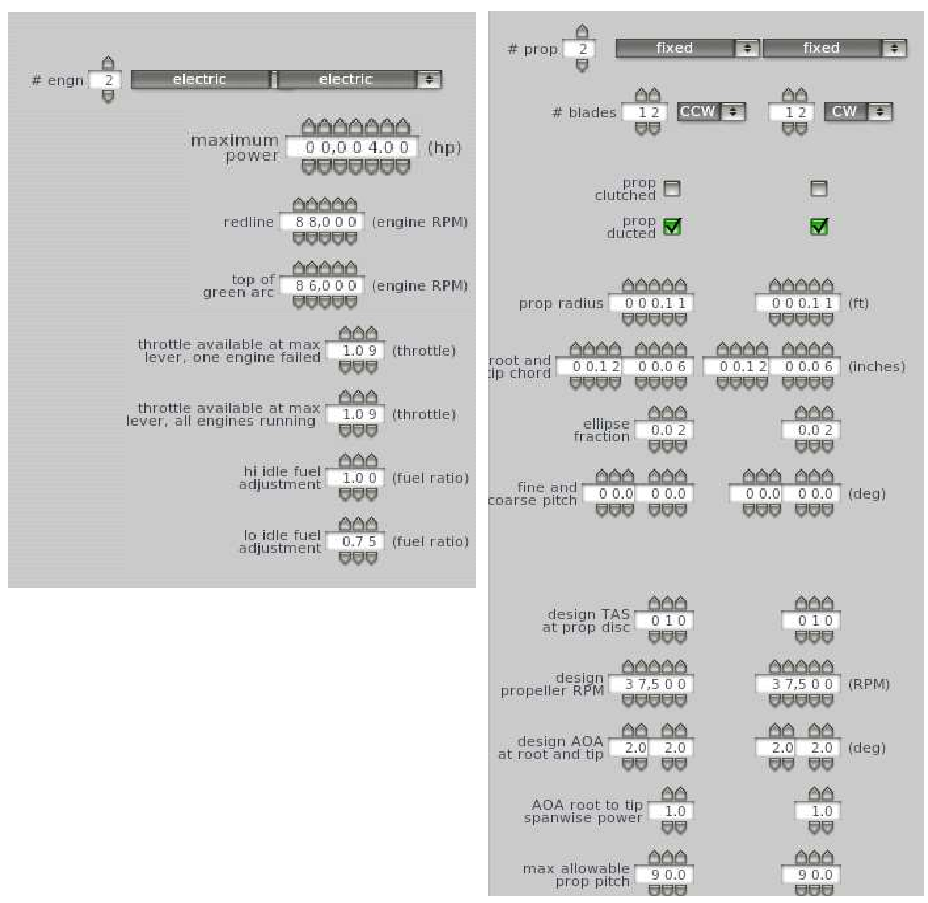
\includegraphics[scale=0.7]{Capitulo3/figs/espf motores.pdf}
    \caption{Especificaciones de motores}
    \label{Especificaciones de motores}
\end{figure}
En la figura \ref{Especificaciones de motores} se observan las principales configuraciones de los motores eléctricos y de las hélices o propelas. 
A continuación se explican la parametrización del sistema de propulsión. 
\begin{itemize}
    \item Se seleccionan dos motores eléctricos. 
    \item Se configura la potencia máxima de ambos motores eléctricos en 4hp, es decir, cada motor ofrece 2hp o 1491.4 watts(W). Se considera en aplicación una eficiencia del 90$\%$. 
    \item Las revoluciones máximas de los motores se establecen en 88,000RPM y  una aceleración disponible de 1.09 que indica el 100$\%$ de la capacidad de aceleración.
    \item Se establece la razón o ajuste de combustible o energía, que se refiere al proceso de configurar la cantidad de energía (en el caso de nuestra batería eléctrica) que libera la fuente de poder al motor durante altas y bajas velocidades de operación. Para altas velocidades se establece una razón de 1 y para bajas velocidades una razón de 0.75. 
\end{itemize}

Ahora vamos a explicar el segundo bloque de la Figura \ref{Especificaciones de motores} correspondiente a las especificaciones de las hélices de los fan dentro de los ductos. 
\begin{itemize}
    \item Se seleccionan dos fans fijos (uno para cada motor).
    \item Se colocaron 12 hélices. El radio de las hélices se establece en 0.11ft o 33.5mm aproximadamente. Está consideración es para motores ductofan alrededor de 70mm de diámetro, dónde también 80mm y 90mm son comunes.
\end{itemize}
  
Además de las características de los motores y de las hélices que componen el fan dentro del ducto, las características del sistema eléctrico son fundamentales en el desarrollo de un VANT. 
El sistema eléctrico se configuro con las dos baterías eléctricas propuestas en la sección \ref{superficie alar y potencia requerida}, dónde cada batería ofrece 0.146 watt-hora, y el diseño del generador tiene una razón de 0.25 RPM. 


En la Figura \ref{Centro de gravedad y peso de EHEKATL BWB} se muestra la ubicación del centro de gravedad, la masa en vacío y máxima y la parametrización del tren de aterrizaje. 
\begin{figure}[!t]
    \centering
    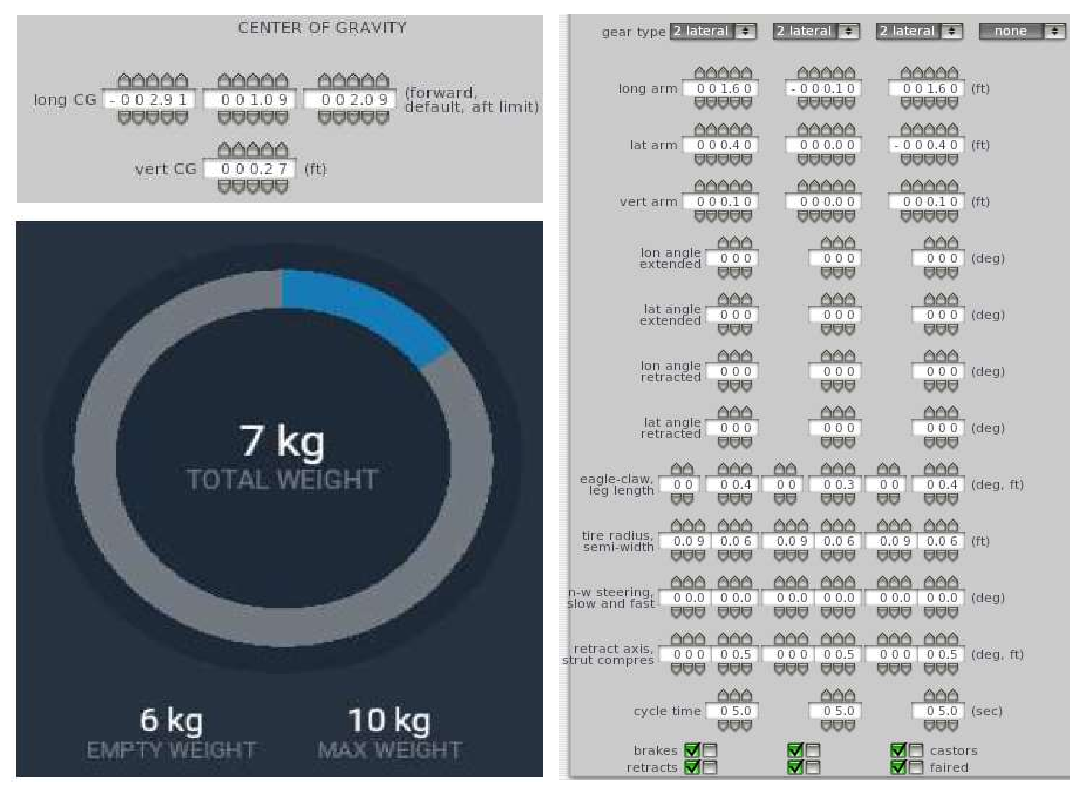
\includegraphics[scale=0.7]{Capitulo3/figs/weight and landing gear.pdf}
    \caption{Centro de gravedad y peso de EHEKATL BWB}
    \label{Centro de gravedad y peso de EHEKATL BWB}
\end{figure}
En la Figura \ref{Centro de gravedad y peso de EHEKATL BWB} se configuran las coordenadas del centro de gravedad y justo debajo la masa en vacío y la masa máxima. La masa en vacío se establece en 6kg pero más bien como masa mínima de EHEKATL BWB, y 10kg como efectivamente como masa máxima. Se establece la masa de 7kg para fines de simulación. 
Finalmente, se configura el tren de aterrizaje. Se seleccionan tres sistemas para tren de aterrizaje. De izquierda a derecha, la primer columna configura el tren trasero del lado izquierdo, la segunda el tren delantero central próximo a la nariz y el tercero tren también trasero pero del lado derecho. 
Se establecen trenes de aterrizaje de doble rueda. En las siguientes tres filas se establecen las coordenadas de la ubicación para cada tren. 
Posteriormente se configura el parámetro \textit{eagle-claw, leg length} que hace referencia al largo de la pata del tren cuando se encuentra extendido. 
Posteriormente, se configura el \textit{tire radius} que corresponde con el radio de la llanta y \textit{semi-with} que corresponde con el semi-ancho de la misma llanta.
Por último, se ajustan las especificaciones para el sistema retráctil, dónde \textit{retract axis, strut compres} refiere a la cantidad de compresión de la pata del tren durante el ciclo de retracción. Se establece un ciclo de retracción de cinco segundos, y en la parte final del bloque se selecciona la opción retráctil con sistema de frenos. 


En el panel de la cabina de EHEKATL BWB se implementaron 26 instrumentos de navegación, ver Figura \ref{Panel de Cabina de EHEKATL BWB}.
A continuación se menciona cada instrumento y su uso.

1) Indicador de frenos. Prende en rojo la palabra \textit{brake} cuando los frenos están activados. 2) Mach. De manera análoga muestra la velocidad de acuerdo al Mach. 3) Nivel de inclinación o deslizamiento. La burbuja sale del centro respecto a la inclinación lateral del ala. 4) Indicador de desplome. Indica cuando la aeronave se encuentra en situación de pérdida (fuera de control). 5) Indicador de poder de motores. Muestra en $hp$ la potencia dada por los motores.
6) Pérdida respecto al ángulo de ataque. Indica de manera radial cuando se encuentra en un ángulo de ataque estable y cuando trasciende a un ángulo de ataque que provoca desplome. 7) Ángulo de ataque en aterrizaje. Indica mediante tres luces si la aeronave debe mantener, subir o bajar el ángulo de ataque para un aterrizaje suave. 8) Indicador del ángulo de ataque. Muestra el ángulo de ataque de manera lineal en grados. 9) Ventana de horizonte. Muestra la línea de horizonte y la inclinación del ala y de la nariz respecto a este en grados. 10) Indicador de la velocidad el aire. Indica de manera lineal la velocidad del aire en nodos. 
11) Régimen de ascenso. Velocidad vertical o de ascenso mostrada de manera lineal y en grados. 12) Altímetro. Indica la altura respecto al nivel del mar en pies. 13) Altímetro. Indica la altura respecto a tierra mediante un rada en pies. 14) Indicador del ángulo de deslizamiento. Indica el ángulo de derrape en grados. 15) Compas. Instrumento más antiguo de navegación. 
\begin{figure}[!t]
    \centering
    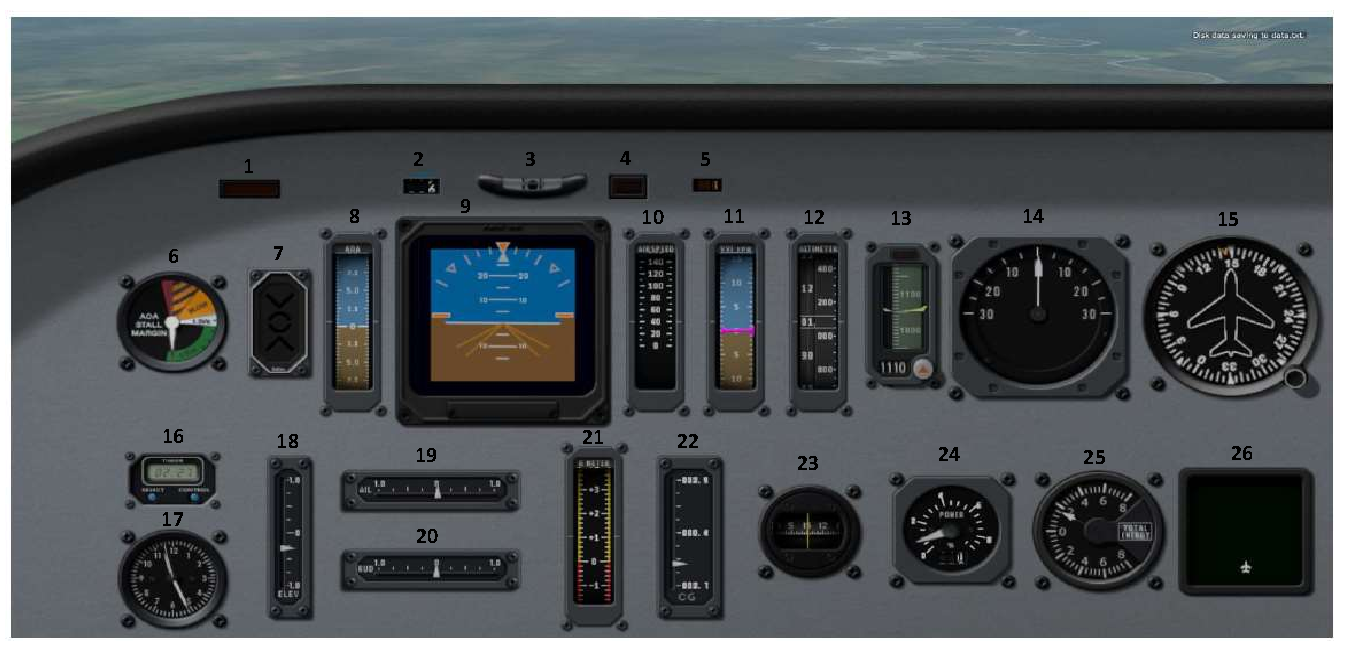
\includegraphics[scale=0.6]{Capitulo3/figs/paneles ehekatl 2.pdf}
    \caption{Panel de Cabina de EHEKATL BWB}
    \label{Panel de Cabina de EHEKATL BWB}
\end{figure}
16) Cronómetro. Medir el tiempo de vuelo. 17) Reloj. simple reloj análogo.  18) Indicador de deflexión de elevadores. Indica la deflexión de los elevadores en una escala de 1 a -1, siendo cero ninguna deflexión. 19) Indicador de deflexión de alerones. 20) Indicador de deflexión de timón. 21) Fuerzas G. Indicador lineal de las fuerzas G. 22) Centro de gravedad. Indicador lineal de la posición del centro de gravedad. 23) Compas. Similar al anterior pero con un diseño lineal en lugar de radial. 24) Indicador de poder. Muestra el poder de los motores. 25) Muestra el total de energía potencial y cinética de la aeronave. 26) Radar. Muestra en color verde vehículos aéreos próximos. 

Si bien EHEKATL BWB esta pensando para ser un VANT, la misma instrumentación se puede monitorear en tiempo real en un sistema en tierra.

\begin{figure}[!t]
    \centering
    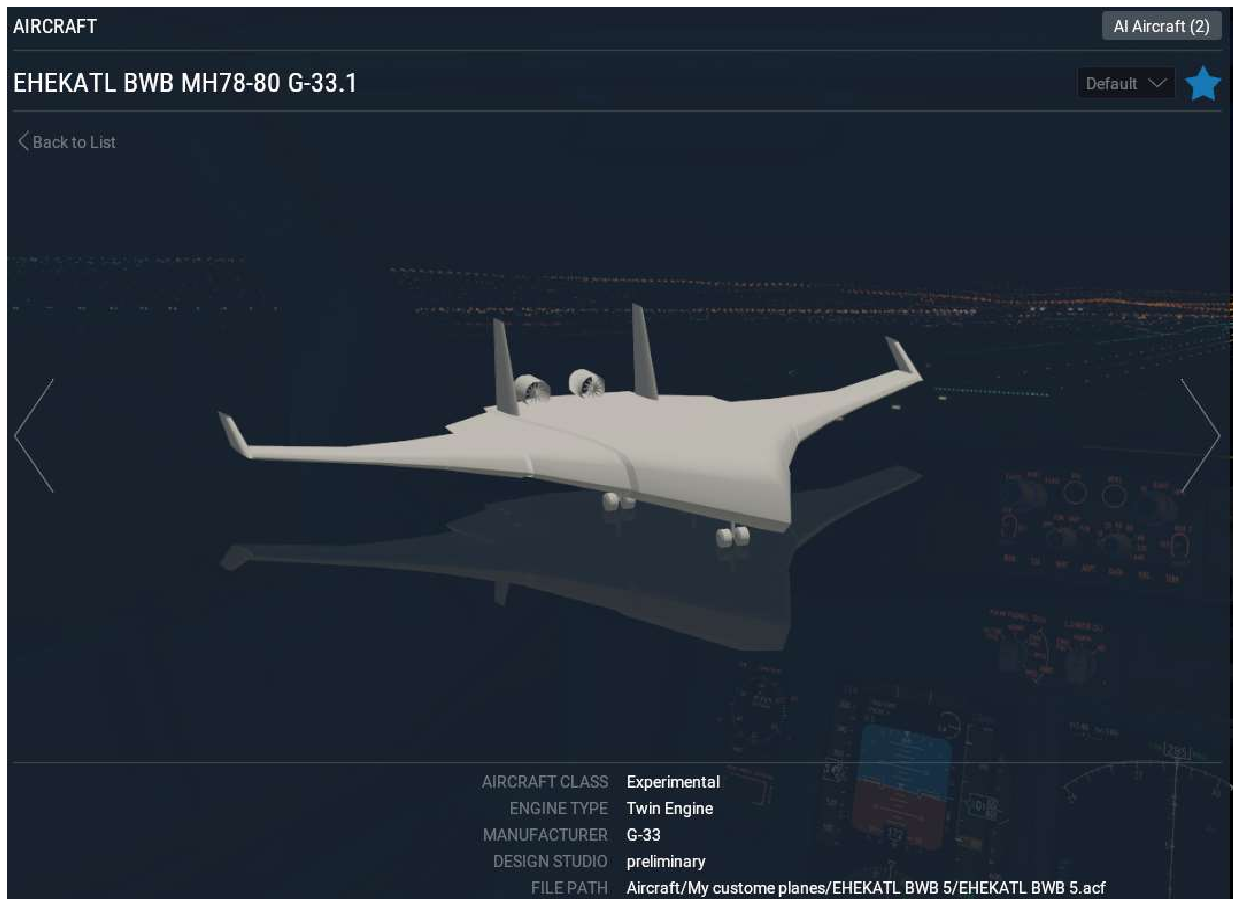
\includegraphics[scale=0.66]{Capitulo3/figs/Datos generales.pdf}
    \caption{EHEKATL BWB en el entorno del simulador de vuelo X-PLANE}
    \label{Datos generales de EHEKATL BWB G-33}
\end{figure}

En la Figura \ref{Datos generales de EHEKATL BWB G-33} se observa el modelo final de EHEKATL BWB realizado en Plane Maker dentro del entorno del simulador de vuelo X-PLANE. 

\section{Discusiones}

La definición clara y precisa de la misión de vuelo es un paso fundamental en el diseño de cualquier aeronave. Utilizar la atmósfera estándar internacional es una buena primera aproximación para determinar la presión, densidad y temperatura del aire en función de la altitud dónde se planea realizar la misión de vuelo. 

La selección y análisis de perfiles aerodinámicos en XFLR5 permite una evaluación detallada de las características de sustentación y resistencia de la aeronave. La elección de perfiles para aeronaves BWB es crucial, dónde además de buscar un buen desempeño aerodinámico se necesita considerar la estabilidad en cabeceo. 

El proceso de diseño de perfiles aerodinámicos en Airfoil Maker complementa la evaluación realizada en XFLR5. Lograr el mismo comportamiento entre los resultados obtenidos con XFLR5 y el diseño en Airfoil Maker es esencial para lograr un diseño posterior en Plane Maker consistente y simulaciones en X-PLANE con buenas aproximaciones. 

La aplicación de XFLR5 para el análisis aerodinámico proporciona valiosa información sobre la distribución de presiones y flujo alrededor de la aeronave. Este análisis contribuye a la comprensión detallada del comportamiento aerodinámico de la EHEKATL BWB y permite realizar ajustes en el diseño para mejorar el rendimiento.

La evaluación de la estabilidad y control de EHEKATL BWB en XFLR5 es un paso crítico para garantizar la maniobrabilidad y seguridad durante el vuelo. Los resultados de este análisis influyen en la configuración de superficies de control y sistemas de estabilización.

La implementación del diseño conceptua en Plane Maker representa un hito significativo en el proceso de desarrollo de la aeronave. Esta etapa permite la traducción de los conceptos teóricos y datos aerodinámicos en un modelo virtual funcional, lo cual facilita la simulación y prueba de vuelo.

La revisión detallada de los pasos de diseño presentados en este capítulo proporciona una base para la implementación práctica y refinamiento de la aeronave de EHEKATL BWB. Los resultados de los análisis aerodinámicos y de estabilidad influyen en las decisiones de diseño y en la configuración final de la aeronave, recordando el proceso iterativo en el diseño de aeronaves. 















%%%%%%%%%%%%%%%%%%%%%%%%%%%%%%%%%%%%%%%%%%%%%%%%%%%%%%%%%%%%%%%%%%%%%%%%
%           Capítulo 3: Modelado de la Aeronave               %
%%%%%%%%%%%%%%%%%%%%%%%%%%%%%%%%%%%%%%%%%%%%%%%%%%%%%%%%%%%%%%%%%%%%%%%%%
\chapter{Modelado Dinámico}

Una vez realizado el diseño aerodinámico, en este capítulo se presenta el modelo dinámico de EHEKATL BWB. 
Dado que las aeronaves son consideradas sistemas dinámicos complejos durante su operación en vuelo y no son estables por sí mismas, necesitan de un sistema de control para volar en la dirección deseada y compensar perturbaciones.
%
 Para el modelado dinámico de EHEKATL BWB vamos a considerar un cuerpo rígido de seis grados de libertad; tres grados de desplazamiento (hacia adelante, hacia un lado y hacia abajo) y tres grados de rotación (cabeceo, alabeo y guiñada).
De tal forma, se tendrán seis ecuaciones diferenciales, basadas en las leyes Newtonianas, que gobernarán el movimiento de la aeronave. 
%
Para el desarrollo del modelo dinámico se propone EHEKATL BWB con dos motores, ocho superficies de control aerodinámicas en el borde de fuga y dos timones direccionales en los estabilizadores verticales.
%
En \ref{modelado TVC}, se propone el modelado para EHEKATL BWB TVC considerando una tobera con deflexión para generación de momentos de cabeceo y guiñada. 
  
%%%%%%%%%%%%%%%%%%%%%%%%%%%%%%%%%%%%%%%%%%%%%%%%%%%%%%%%%%%%%%%%
\section{Sistemas de Referencia}
%%%%%%%%%%%%%%%%%%%%%%%%%%%%%%%%%%%%%%%%%%%%%%%%%%%%%%%%%%%%%%%%

Un \textbf{Sistema de Referencia Inercial} es un campo donde se cumplen la segunda ley de la dinámica de Newton. Podemos decir que la variación en el momento lineal y/o angular del sistema es igual a las fuerzas reales que actúan sobre el sistema, esto quiere decir que se considera al sistema en reposo o en movimiento relativo uniforme al menos que una fuerza externa actúe en él. Como contraste, un \textbf{Sistema de Referencia No Inercial} es aquel que respecto a un sistema inercial está moviéndose con aceleración, en este campo no se cumplen las leyes de Newton. En un Sistema No Inercial es necesario introducir el término de fuerzas ficticias (algunas fuerzas ficticias pueden ser la fuerza de Coriolis o la fuerza centrífuga).
%
Los \textbf{sistemas de referencia terrestres} que se utilizan son: 
\begin{itemize}
    \item Centro-Terrestre Inercial $(i)$
    \item Centro-Terrestre Fijo $(e)$
    \item Geodésico Local $(\lambda, \phi, h)$
\end{itemize}
El Sistema de Referencia de Centro-Terrestre Fijo (ECEF), también conocido como Sistema de Referencia Geocéntrico, rota a la velocidad real de la Tierra respecto al Sistema de Referencia Centro-Terrestre Inercial (ECI) que representa los ejes de coordenadas inerciales no rotacionales. 
El ECI es denotado por $(i)$ mientras ECEF por $(e)$. Ambos son ortogonales y tienen su origen en el centro de la tierra. 
Los ejes $z_{i,e}$ están alineados como eje fijo al vector de rotación Terrestre, mientras que $x_{i,e}, y_{i,e}$ se localizan en el plano ecuatorial, con $x_i$ fijo en alguna dirección con referencia celestial, por ejemplo, una línea que conecte al centro del sol respecto a la posición de la tierra en equinoccio de primavera. 
El eje $x_e$ usualmente se intersecta con el meridiano de Greenwich a nivel del ecuador, dónde el eje $y_e$ completa el sistema de la mano derecha. 
La definición del ECEF puede variar, pero siempre debe seguirse la regla de dos vectores en dirección de la rotación terrestre, ver Figura \ref{Sistemas de Referencia Terrestres}.
  
\begin{figure}[!t]
\centering
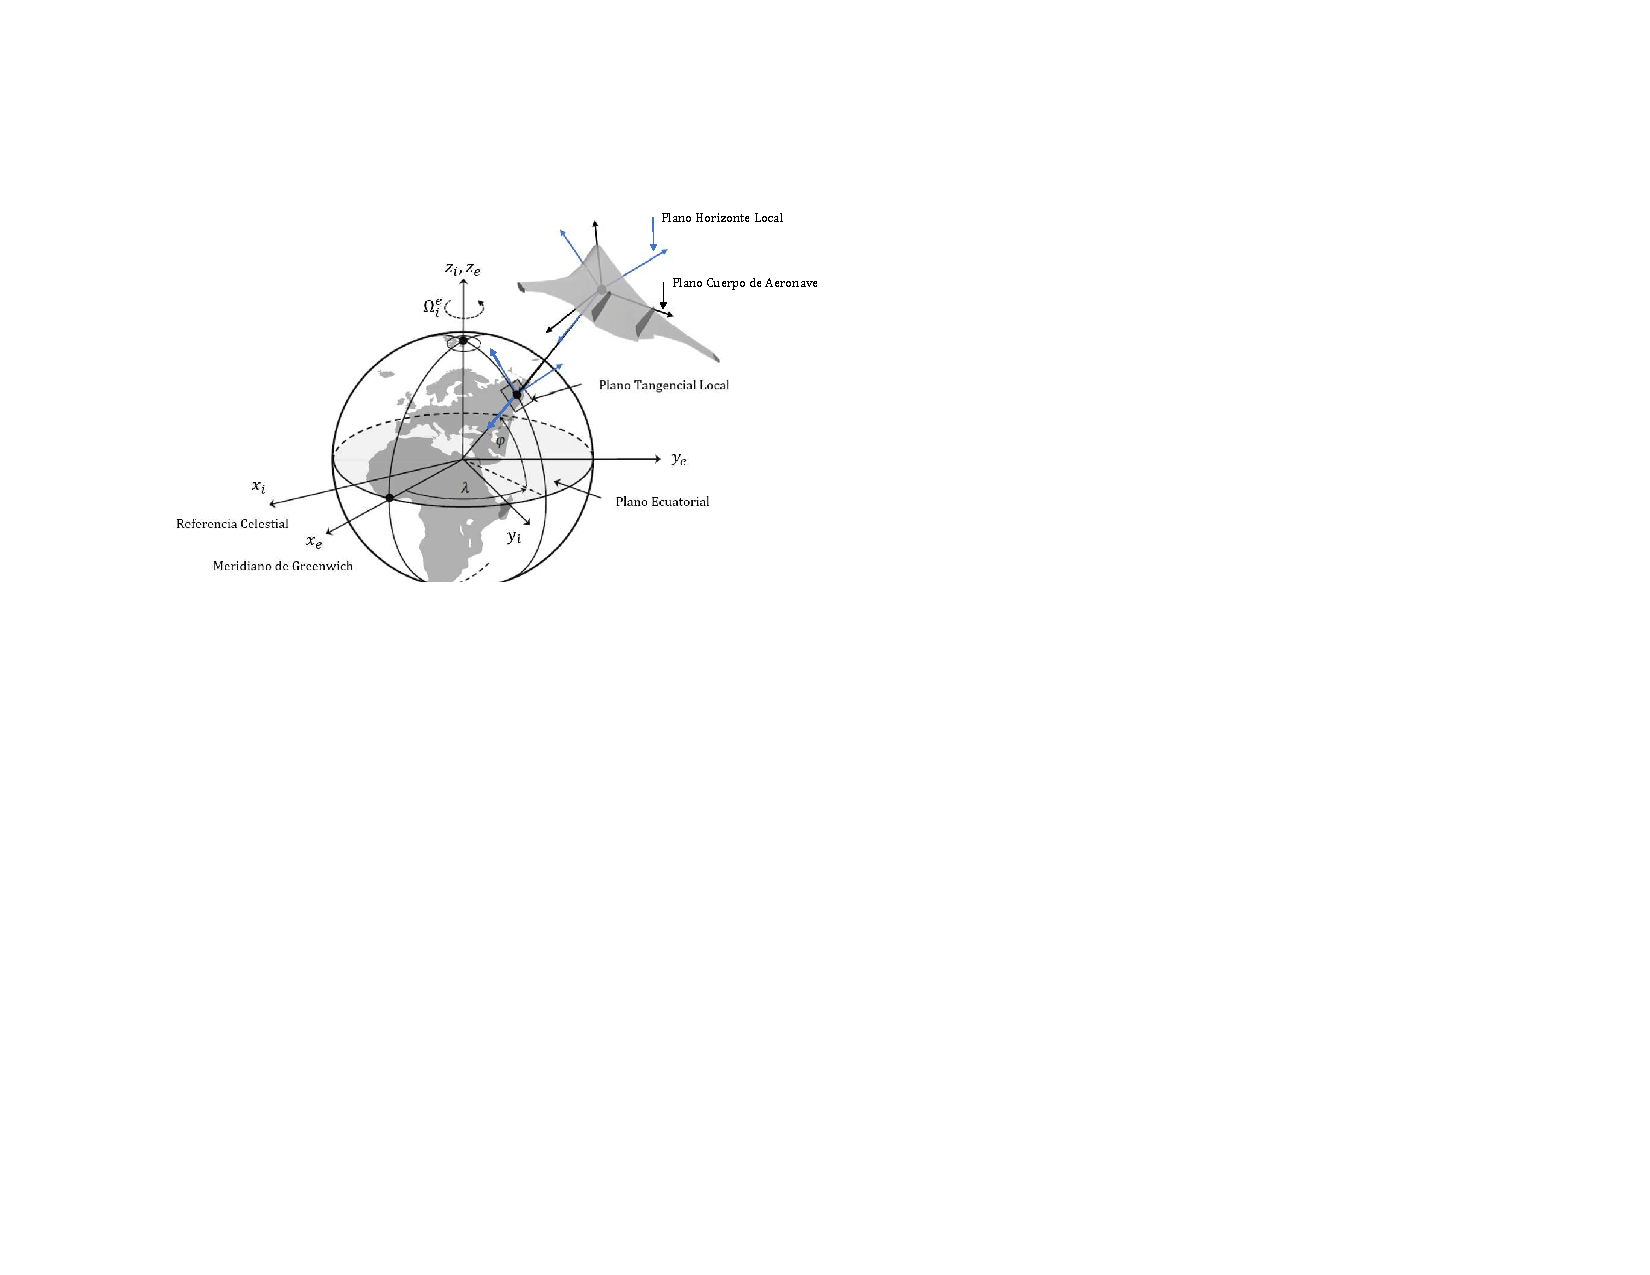
\includegraphics[scale=1.22]{Capitulo3/figs/Sistema de referencia Full_cropped (2).pdf}
\caption{Sistemas de Referencia Terrestres}
\label{Sistemas de Referencia Terrestres}
\end{figure}

Para definir la dinámica de EHEKATL BWB respecto a la tierra, se definen lo siguientes sistemas de referencia que pueden emplearse en distintas tipos de aplicaciones, ver Figura \ref{Sistema de Referencia de EHEKATL BWB}:
\begin{itemize}
    \item Plano Tangencial Local $(t)$
    \item Plano de Horizonte Local $(h)$
    \item Plano Cuerpo de la Aeronave $(b)$
    \item Plano de Estabilidad o Viento $(w)$
\end{itemize}
El origen de los ejes de coordenadas del plano tangencial local (LTP) es fijo a la tierra con dos de sus ejes adjuntos al plano tangencial de la superficie. 
El principal propósito de este plano es como referencia inercial para vuelos de baja duración y velocidad. 
Los ejes $x_t$ y $y_t$ adjuntos a la superficie están en dirección norte y este respectivamente, mientras el eje $z_u$ en dirección hacia el centro de la tierra (abajo). Por lo anterior este sistema de coordenadas también es conocido como (NED) por sus siglas en inglés de \textit{North, East, Down} de acuerdo con las direcciones de sus ejes en la rosa náutica. El origen del LTP usualmente se define por la latitud, longitud y altitud geodésica.  

\begin{figure}[!t]
\centering
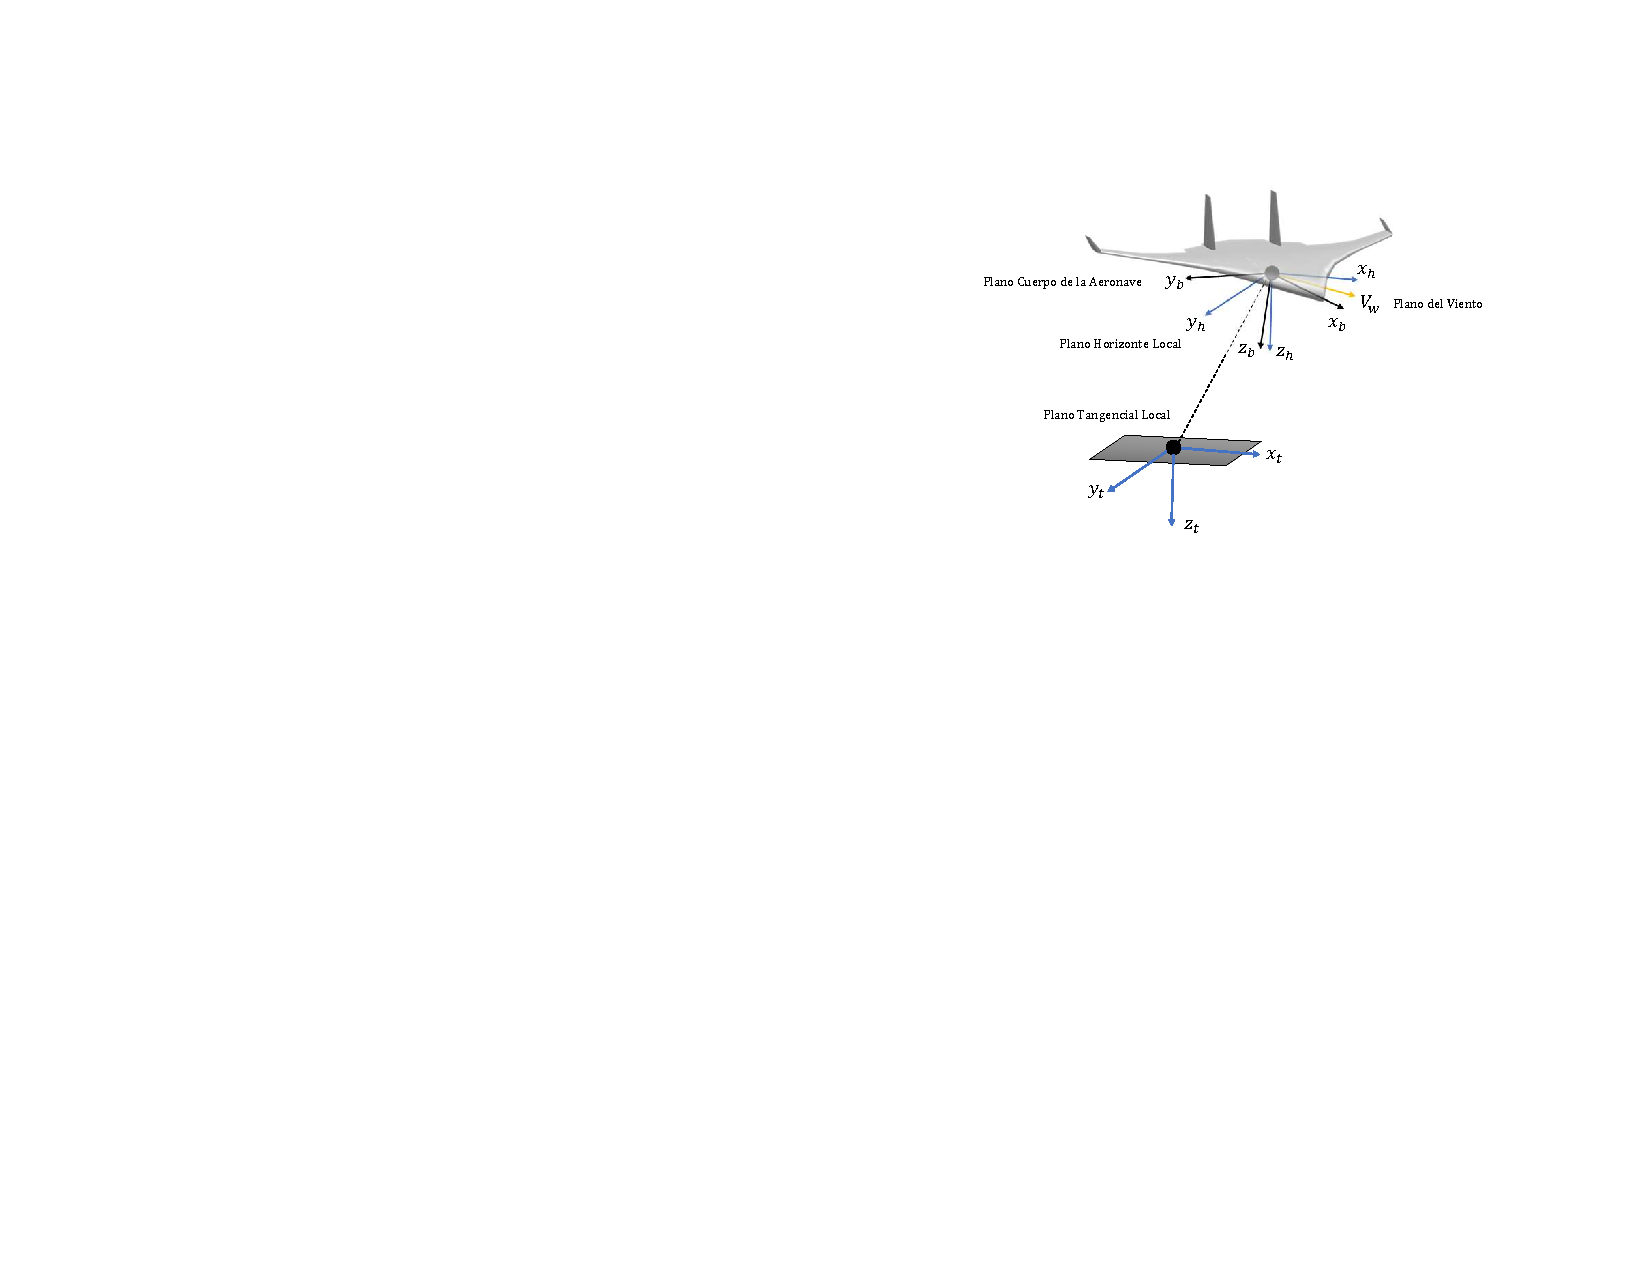
\includegraphics[scale=1.3]{Capitulo3/figs/Sistema de referencia Full_cropped (1).pdf}
\caption{Sistema de Referencia de EHEKATL BWB}
\label{Sistema de Referencia de EHEKATL BWB}
\end{figure}

El origen de las coordenadas de plano horizonte local y plano cuerpo de la aeronave se ubican en el centro de gravedad de la aeronave.

Las coordenadas del plano horizonte local están permanentemente en la misma orientación que el plano tangencial local. La transformación del plano horizonte local respecto al plano tangecial local define la posición después de traslación de la aeronave.  

Las coordenadas plano cuerpo de la aeronave son un sistema de referencia ortogonal fijo al cuerpo de la aeronave, por lo que podemos medir las rotaciones de los ejes 
 del plano cuerpo de la Aeronave respecto a los ejes del plano horizonte local.

Las fuerzas y momentos aerodinámicos resultantes de la interacción aeronave-aire dependen de la orientación del cuerpo de la aeronave con el vector de velocidad del aire. La magnitud del vector de velocidad del aire es opuesto al vector de velocidad definido en LTP con respecto a la velocidad en tierra, por lo que este vector es quien rige la trayectoria de la aeronave. 

%%%%%%%%%%%%%%%$%%%%
\section{Cinemática}
La cinemática estudia el movimiento de un cuerpo de acuerdo con su posición y estado sin importar las causas que lo originan.

La transformación o relación entre los distintos sistemas de referencia es el enfoque central de la cinemática para conocer los movimientos de traslación y rotación de la aeronave. 
%
A partir de los movimientos en el plano cuerpo de la aeronave respecto al plano de horizonte horizontal podemos conocer la actitud de la aeronave en el tiempo, y multiplicando la matriz de transformación por las velocidades lineales de cada eje podemos obtener la \textbf{matriz de navegación}. 
%
La implementación de los planos tangencia local, horizonte local, cuerpo de la aeronave y de viento permiten determinar los cambios de posición y orientación de EHEKATL BWB. 

\bigskip
%%%%%%%%%%%%%%%%%%%%%%%%%%%%%%%%%%%%%%%%%%%%%%%%%%%%%%%%%%%%%%%%%%%%%%%%%%%%%%%%%%%%%
\textbf{ Cinemática Traslacional y Rotacional}\\
%%%%%%%%%%%%%%%%%%%%%%%%%%%%%%%%%%%%%%%%%%%%%%%%%%%%%%%%%%%%%%%%%%%%%%%%%%%%%%%%%%%
Los sistemas de coordenadas considerados en la \textbf{actitud de los ángulos de Euler} están basados en el plano de horizonte local y plano cuerpo de la aeronave. 
%
Se tienen tres grados de libertad en la cinemática rotacional (cabeceo, alabeo y guiñada) y tres grados de libertad en la cinemática traslacional (axial, normal y lateral).
%
Primero, se estudia la cinemática rotacional. Un teorema de Euler establece que: “Cualquier número de rotaciones respecto a diferentes ejes desde un punto similar, al final, debe identificarse como una simple rotación”.\\
La secuencia de transformación se expresa a continuación. 

\begin{figure}[h]
\centering
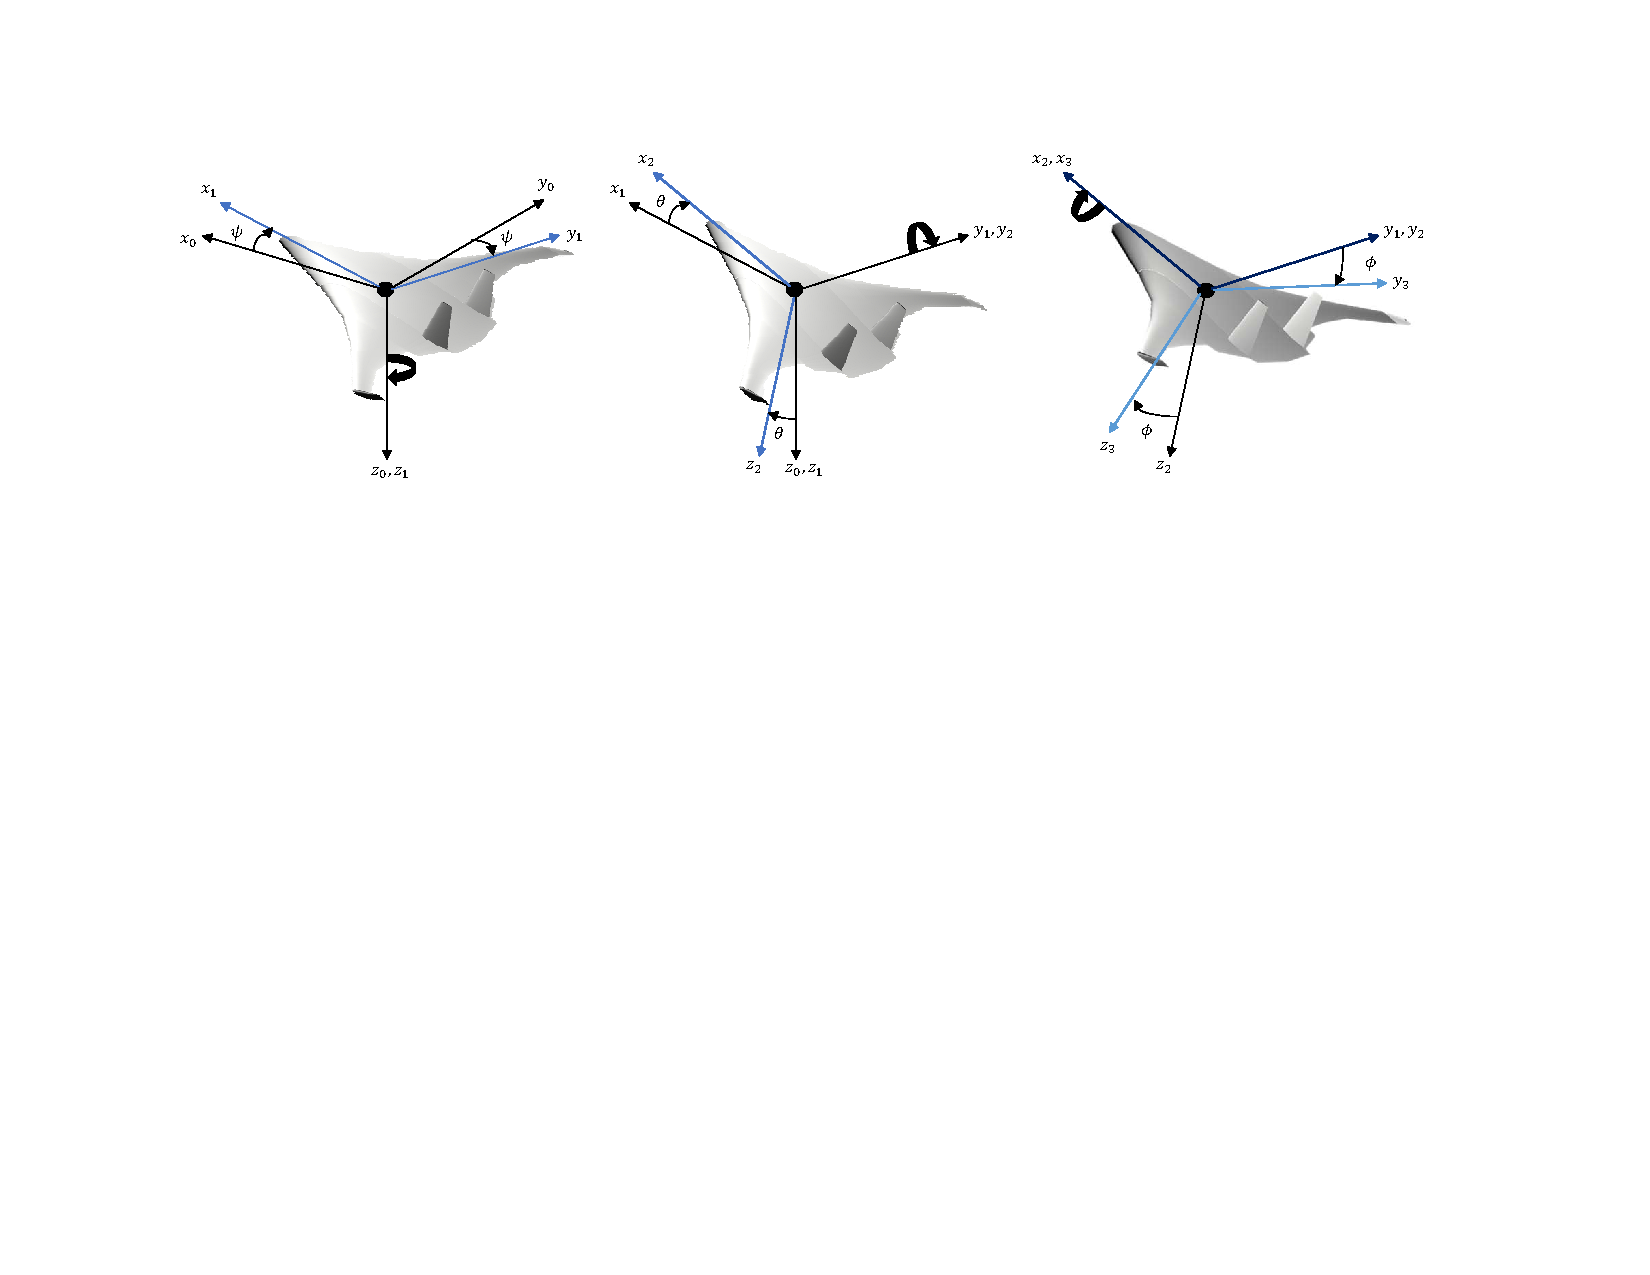
\includegraphics[scale=0.63]{Capitulo3/figs/cinematica ehekatl 1_cropped (1).pdf}
\caption{Secuencia de rotación: guiñada, cabeceo y alabeo}
\label{fig: secuencia de rotación}
\end{figure}

\begin{equation}
    X_{0} \Rightarrow T_{\psi} \Rightarrow X_{1} \Rightarrow T_{\theta} \Rightarrow X_{2} \Rightarrow T_{\phi} \Rightarrow X_{3}
\end{equation}
Todas las rotaciones son positivas siguiendo la regla de la mano derecha.

La transformación del vector $X_{0} \Rightarrow T_{\psi} \Rightarrow X_{1}$ se expresa en notación matricial como:

\begin{gather}
    \begin{bmatrix}
    x_{1}\\
    y_{1}\\
    z_{1}
    \end{bmatrix}
    =
    \begin{bmatrix}
    C_{\psi} & S_{\psi} & 0\\
    -S_{\psi} & C_{\psi} & 0\\
    0 & 0 & 1
    \end{bmatrix}
    \begin{bmatrix}
    x_{0}\\
    y_{0}\\
    z_{0}
    \end{bmatrix}
\end{gather}

\begin{equation}
    X_{1} = T_{\psi}X_{0},\quad X_{0}= T^T_{\psi}X_{1}
\end{equation}

La transformación del vector $X_{1} \Rightarrow T_{\theta} \Rightarrow X_{2}$ se expresa en notación matricial como:

\begin{gather}
    \begin{bmatrix}
    x_{2}\\
    y_{2}\\
    z_{2}
    \end{bmatrix}
    =
    \begin{bmatrix}
    C_{\theta} & 0 & -S_{\theta}\\
    0 & 1 & 0\\
    S_{\theta} & 0 & C_{\theta}
    \end{bmatrix}
    \begin{bmatrix}
    x_{1}\\
    y_{1}\\
    z_{1}
    \end{bmatrix}
\end{gather}

\begin{equation}
    X_{2} = T_{\theta}X_{1},\quad X_{1}= T^T_{\theta}X_{2}
\end{equation}

La transformación del vector $X_{2} \Rightarrow T_{\phi} \Rightarrow X_{3}$ se expresa en notación matricial como:

\begin{gather}
    \begin{bmatrix}
    x_{3}\\
    y_{3}\\
    z_{3}
    \end{bmatrix}
    =
    \begin{bmatrix}
    1 & 0 & 0\\
    0 & C_{\phi} & S_{\phi}\\
    0 & -S_{\phi} & C_{\phi}
    \end{bmatrix}
    \begin{bmatrix}
    x_{2}\\
    y_{2}\\
    z_{2}
    \end{bmatrix}
\end{gather}

\begin{equation}
    X_{3} = T_{\phi}X_{2},\quad X_{2}= T^T_{\phi}X_{3}
\end{equation}

La transformación final del plano cuerpo de la aeronave respecto al plano de horizonte local es la multiplicación ordenada de las matrices de transformación individuales mostradas como:

\begin{figure}[h]
\centering
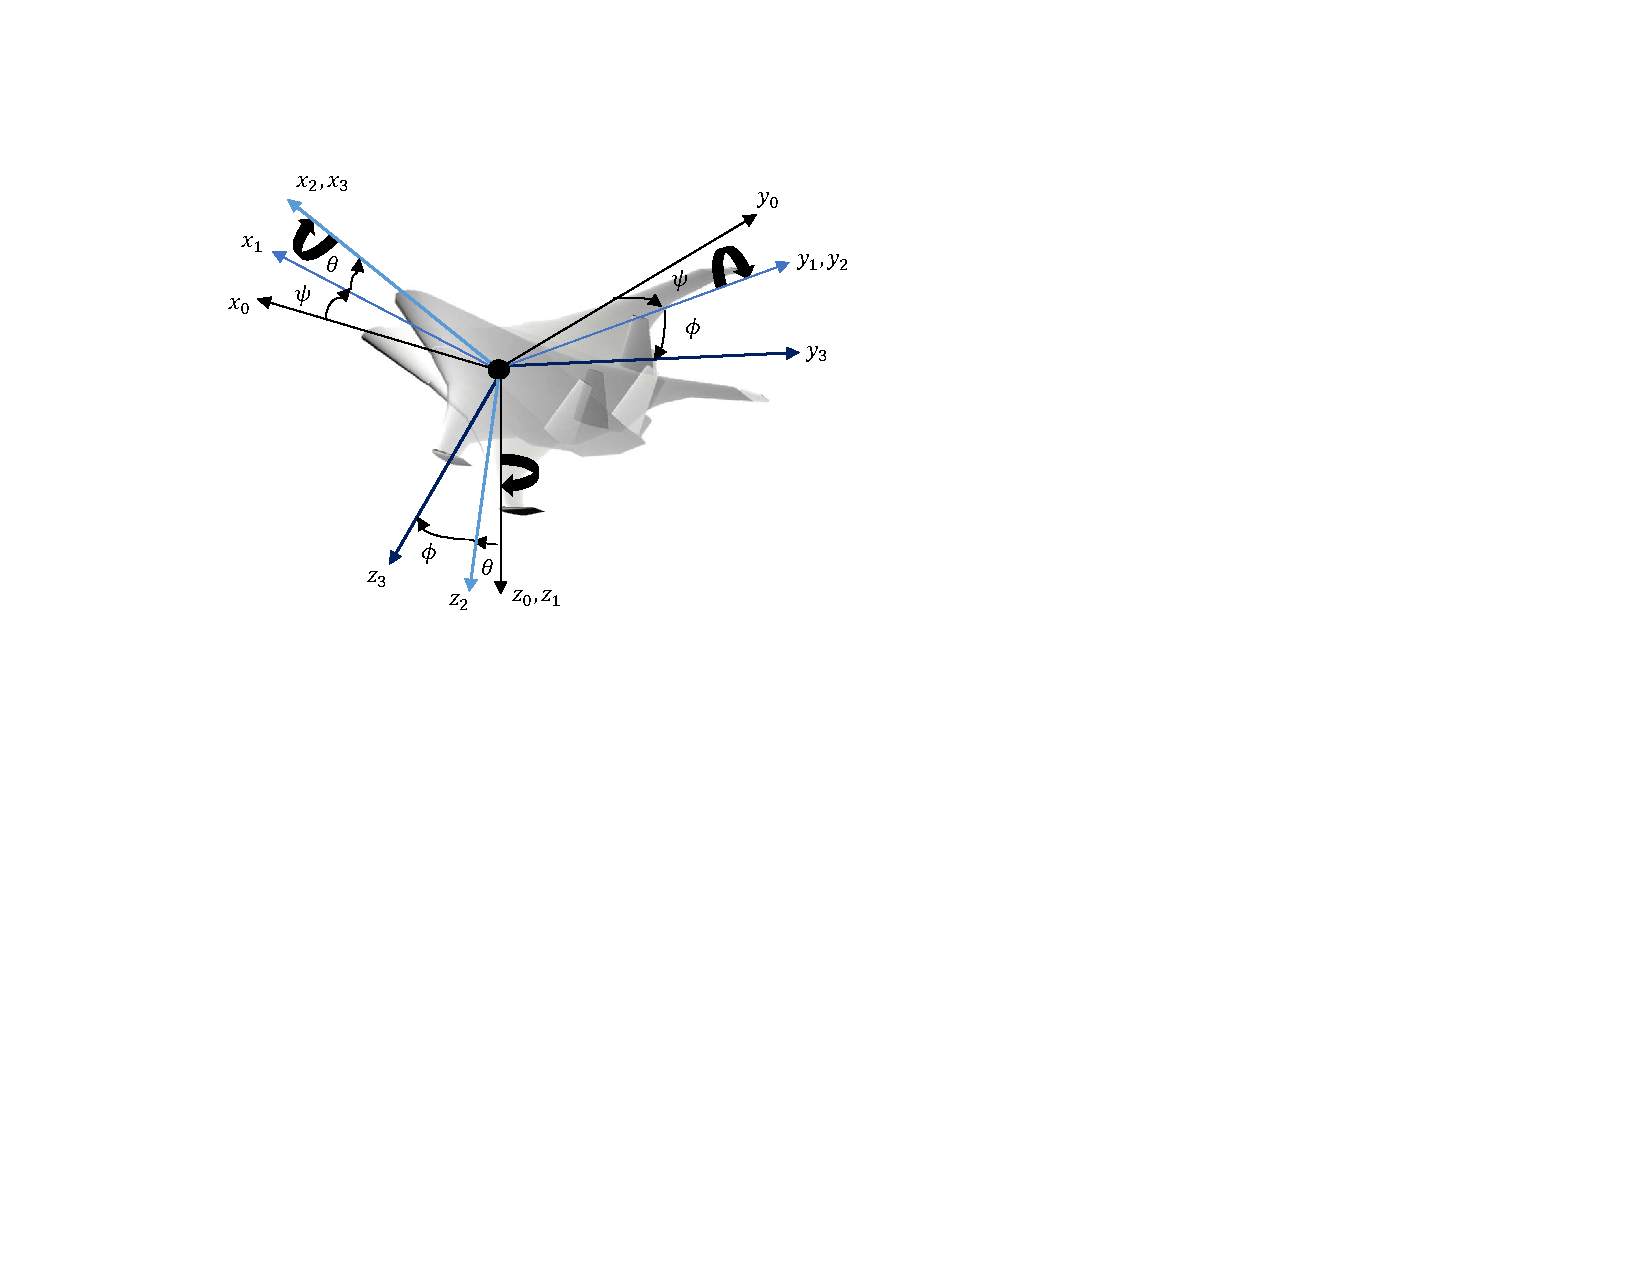
\includegraphics[scale=1]{Capitulo3/figs/cinematica ehekatl 2_cropped.pdf}
\caption{Secuencia de rotación de los ángulos de Euler}
\label{fig:x cubed graph}
\end{figure}


\begin{gather}
    \begin{bmatrix}
    x_{b}\\
    y_{b}\\
    z_{b}
    \end{bmatrix}
    =
    T_{\psi} T_{\theta} T_{\phi} 
    \begin{bmatrix}
    x_{n}\\
    y_{n}\\
    z_{n}
    \end{bmatrix}
\end{gather}

\begin{gather}
    \begin{bmatrix}
    x_{n}\\
    y_{n}\\
    z_{n}
    \end{bmatrix}
    =
    \begin{bmatrix}
    T_{\psi} & T_{\theta} & T_{\phi} 
    \end{bmatrix} ^T
    \begin{bmatrix}
    x_{b}\\
    y_{b}\\
    z_{b}
    \end{bmatrix}
\end{gather}

Por simplificación diremos que $S = T_{\psi} T_{\theta} T_{\phi}$, dónde:
\begin{gather}
    S
    =
    \begin{bmatrix}
    C_{\psi} C_{\theta} & S_{\psi} C_{\theta} & -S_{\theta}\\
    C_{\psi} S_{\theta} S_{\phi} - S_{\psi} C_{\phi} & S_{\psi} S_{\theta} S_{\phi} + C_{\psi} C_{\phi} & C_{\theta} S_{\phi} \\
    C_{\psi} S_{\theta} C_{\phi} + S_{\psi} S_{\phi} & S_{\psi} S_{\theta} C_{\phi} - C_{\psi} S_{\phi} & C_{\theta} C_{\phi}
    \end{bmatrix}
\end{gather}

Mientras que:
\begin{gather}
    S^T 
    =
    \begin{bmatrix}
    C_{\psi} C_{\theta} & C_{\psi} S_{\theta} S_{\phi} - S_{\psi} C_{\phi} & C_{\psi} S_{\theta} C_{\phi} + S_{\psi} S_{\phi}  \\
    S_{\psi} C_{\theta} &  S_{\psi} S_{\theta} S_{\phi} + C_{\psi} C_{\phi} & S_{\psi} S_{\theta} C_{\phi} - C_{\psi} S_{\phi} \\
    -S_{\theta} & C_{\theta} S_{\phi} & C_{\theta} C_{\phi} 
    \end{bmatrix}
\end{gather}

Por otro lado, los componentes de velocidad de la aeronave $V_b = [u,v,w]^T$ son conocidos en el cuerpo de la aeronave. Entonces los componentes de la velocidad absoluta en el sistema de referencia inercial pueden ser usados de acuerdo con las relaciones de transformación vistas previamente, sabiendo que $V_{b}$ es conocido, y queremos encontrar $V_{inercial}$ o $V_{h}$, es decir

\begin{gather}
\label{vh 1}
    \begin{bmatrix}
    \dot x_{h}\\
    \dot y_{h}\\
    \dot z_{h}
    \end{bmatrix}
    =
    S^T
    \begin{bmatrix}
    u\\
    v\\
    w
    \end{bmatrix}
\end{gather}

dónde

\begin{gather}
    V_{b}
    =
    \begin{bmatrix}
    u & v & w 
    \end{bmatrix}^T
\end{gather}

\begin{gather}
    V_{h}
    =
    \begin{bmatrix}
    \dot x_{h} & \dot y_{h} & \dot z_{h} 
    \end{bmatrix}^T
\end{gather}

Tal que la ecuación \ref{vh 1} puede expresarse como:
\begin{equation}
    V_{h} = S_{h/b}^{T} V_{b}
\end{equation}

o bien:
\begin{equation}
    V_{b} = S_{b/h} V_{h}
\end{equation}


\textbf{Nota:} La ecuación de $V_{b}$ puede ser integrada con respecto al tiempo buscando obtener la posición en el tiempo del centro de gravedad de la aeronave con respecto al plano inercial. Esta técnica es adecuada para el uso en simuladores cuando se desea seguir la trayectoria de maniobra de la aeronave.
También es necesario saber la historia en el tiempo de los ángulos de Euler, así como las velocidades, para poder obtener una descripción completa para propósitos de simulación.

\medskip

Ahora consideremos la situación dónde una aeronave experimenta una rotación angular dado el vector de velocidad $\Omega$ con sus componentes en el plano cuerpo de la aeronave.

\begin{gather}
    \Omega
    =
    \begin{bmatrix}
    p\\
    q\\
    r
    \end{bmatrix}
\end{gather}

El vector $\Omega$ puede ser descrito por los componentes alineados de las velocidades de los ángulos de Euler $ \dot \phi, \dot \theta, \dot \psi$ definidos por $\Delta \Omega_{\phi} + \Delta \Omega_{\theta} + \Delta \Omega_{\psi}$.

Entonces, cada uno de los términos quedarían descritos como se muestran a continuación.

\begin{gather}
\label{euler1}
    \Delta \Omega_{\phi}
    =
    T_{\phi}
    \begin{bmatrix}
    \dot \phi\\
    0\\
    0
    \end{bmatrix}
\end{gather}

\begin{gather}
    \Delta \Omega_{\theta}
    =
    T_{\phi} T_{\theta}
    \begin{bmatrix}
    0\\
    \dot \theta\\
    0
    \end{bmatrix}
\end{gather}

\begin{gather}
\label{eueler2}
    \Delta \Omega_{\psi}
    =
    T_{\phi} T_{\theta} T_{\psi}
    \begin{bmatrix}
    0\\
    0\\
    \dot \psi
    \end{bmatrix}
\end{gather}

Por tanto podemos definir el vector de velocidades angulares del cuerpo respecto a las velocidades de lo ángulos de Euler de la siguiente manera:

\begin{gather}
\label{velocidad angular aeronave}
    \begin{bmatrix}
    p\\
    q\\
    r
    \end{bmatrix}
    =
    \begin{bmatrix}
    1 & 0 & -S_{\theta}\\
    0 & C_{\phi} & C_{\theta} S_{\phi}\\
    0 & -S_{\phi} & C_{\theta} C_{\phi}
    \end{bmatrix}
    \begin{bmatrix}
    \dot \phi\\
    \dot \theta\\
    \dot \psi
    \end{bmatrix}
\end{gather}

En \ref{euler1}-\ref{eueler2} se utilizó el \textit{el teorema de la adición de velocidades angulares}. El teorema establece que para un vector de velocidad angular coordinado en un sistema de referencia, el vector de velocidad angular resultante de las rotaciones acumuladas es una suma simple de la contribución de cada rotación. Entonces, sí el plano cuerpo de la aeronave es rotado dado el conjunto de los ángulos de Euler en tiempo variante, definido con respecto al plano de horizonte local como sistema de referencia estacionario, podemos determinar los componentes del vector de velocidad angular $\Omega$ como los parámetros del sistema de referencia giratorio.

La diferencia que podemos observar respecto a la transformación de la ecuación de las variables de navegación, es que los componentes de las derivadas de los ángulos de Euler no son normales el uno con el otro, por tanto, la transformación de la ecuación de las velocidades angulares $p,q,r$ no puede resolverse como una matriz ortogonal. Esto impide que podamos utilizar la matriz de cosenos directores y tengamos que seguir la secuencia mostrada en \ref{euler1}-\ref{eueler2}.
Dado que la matriz de transformación es no singular, la inversa existe. De esta manera, obteniendo la inversa de la matriz de transformación de  \ref{velocidad angular aeronave}. 
\begin{gather}
    \begin{bmatrix}
    \dot \phi\\
    \dot \theta\\
    \dot \psi
    \end{bmatrix}
    =
    \begin{bmatrix}
    1 & S_{\phi} tan\theta & C_{\phi} tan\theta\\
    0 & C_{\phi} & -S_{\phi}\\
    0 & S_{\phi} sec\theta & C_{\phi} sec\theta
    \end{bmatrix}
    \begin{bmatrix}
    p\\
    q\\
    r
    \end{bmatrix}
\label{eq cinem rot}
\end{gather}

Una de las desventajas de utilizar los ángulos de Euler son las singularidades definidas en: 
\begin{gather}
    -\pi \leqslant \psi \leqslant \pi \\
    -\pi / 2 \leqslant \theta \leqslant \pi / 2 \\
    -\pi \leqslant \phi \leqslant \pi
\end{gather}

Para solucionar este problema, sobretodo en misiones de vuelo más elaboradas se hace uso de los cuaterniones. 

\medskip
%%%%%%%%%%%%%%%%%%%%%%%%%%%%%%%%%%%%%%%%%%%%%%%%%%%%%%%%%%%%%%%%%%%%%%%%%%%%%%%
\textbf{Vector de Velocidad}\\
La orientación del vector de velocidad con respecto a los ejes-cuerpo de la aeronave establece dos ángulos significativos en la producción de las fuerzas y momentos aerodinámicos, nombrados \textbf{ángulo de ataque $\alpha$} y \textbf{ángulo de deslizamiento o de derrape $\beta$},  \cite{Schimdt1998}.
\begin{figure}[h]
\centering
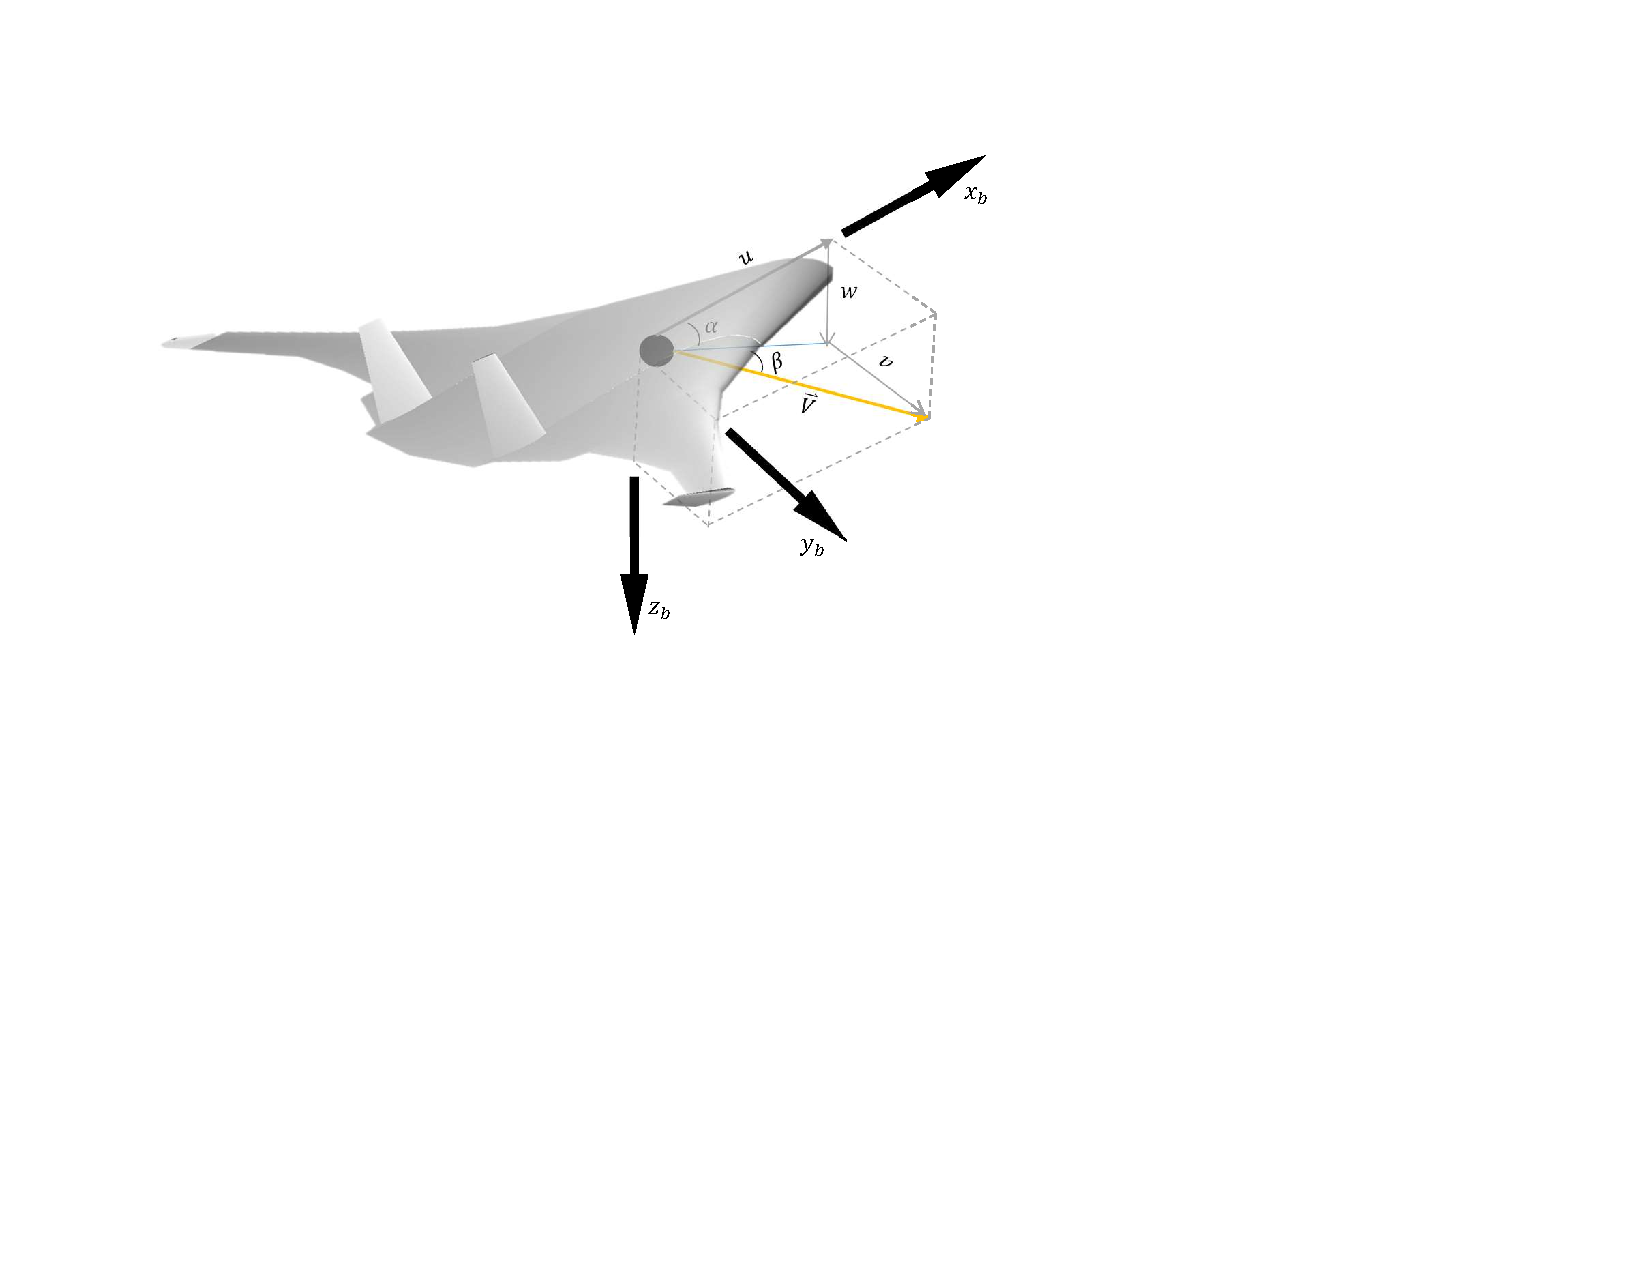
\includegraphics[scale=0.9]{Capitulo3/figs/angulo aerodinamico_cropped.pdf}
\caption{Ángulos aerodinámicos}
\label{fig: angulos aerodinamicos}
\end{figure}

Los componentes de velocidad lineal en el cuerpo de la aeronave $u$,$v$,$w$ se definen como

\begin{align}
\label{eq cossin V}
u &= V C_{\beta} C_{\alpha}\\
v &= V S_{\beta}\\
w &= V C_{\beta} S_{\alpha}
\end{align}

dónde:
\begin{equation}
    V = \sqrt{u^2 + v^2 + w^2}
\end{equation}

El ángulo de ataque $\alpha$ puede obtenerse mediante la función tangente respecto a los componentes en el eje de estabilidad, $u$ y $w$, dando: $tan{(\alpha)}=u/w$.
El ángulo de deslizamiento o derrape $\beta$, es independiente de la dirección de plano de simetría, y se obtiene mediante la componente lateral $v$ que es el cateto opuesto y nuestra hipotenusa o resultante $\Vec{V}$, obteniendo: $sin{\beta}=v/V$.

Los ángulos aerodinámicos del vector de velocidad se definen:

\begin{equation}
\label{eq: angulos aero1}
  \alpha = tan^{-1} \frac{w}{u}  
\end{equation}

\begin{equation}
\label{eq: angulos aero2}
  \beta = sin^{-1} \frac{v}{V}
\end{equation}

\medskip

Para ángulos pequeños asumimos la velocidad inicial como constante, $u_0 = V$, tal que la variación de los ángulos es pequeña (considerando la teoría de las pequeñas perturbaciones) \ref{eq: angulos aero1},\ref{eq: angulos aero2} se re-escriben como: 

\begin{align}
\label{eq: ángulos aerodinámicos con pequeñas perturbaciones}
\alpha &= \frac{w}{u}\\
\beta &= \frac{v}{V}
\end{align}

\medskip
%%%%%%%%%%%%%%%%%%%%%%%%%%%%%%%%%%%%%%%%%%%%%
\textbf{Fuerzas de Levantamiento y Arrastre}\\
A continuación se muestra la transformación del eje de estabilidad respecto al eje cuerpo de la aeronave en el plano de simetría plano $x-z$ usando el vector de fuerzas representado por la suma de los componentes de las fuerzas aerodinámicas de arrastre $D$ y levantamiento $L$.
El vector de fuerzas resultante será entonces reescrito como los componentes de las fuerzas $X$ y $Z$ en los ejes cuerpo de la aeronave.  

Se asume que la aeronave está en vuelo en equilibrio (altitud y velocidad constante), lo que implica que el vector de velocidad es horizontal. 

\begin{figure}[h]
\centering
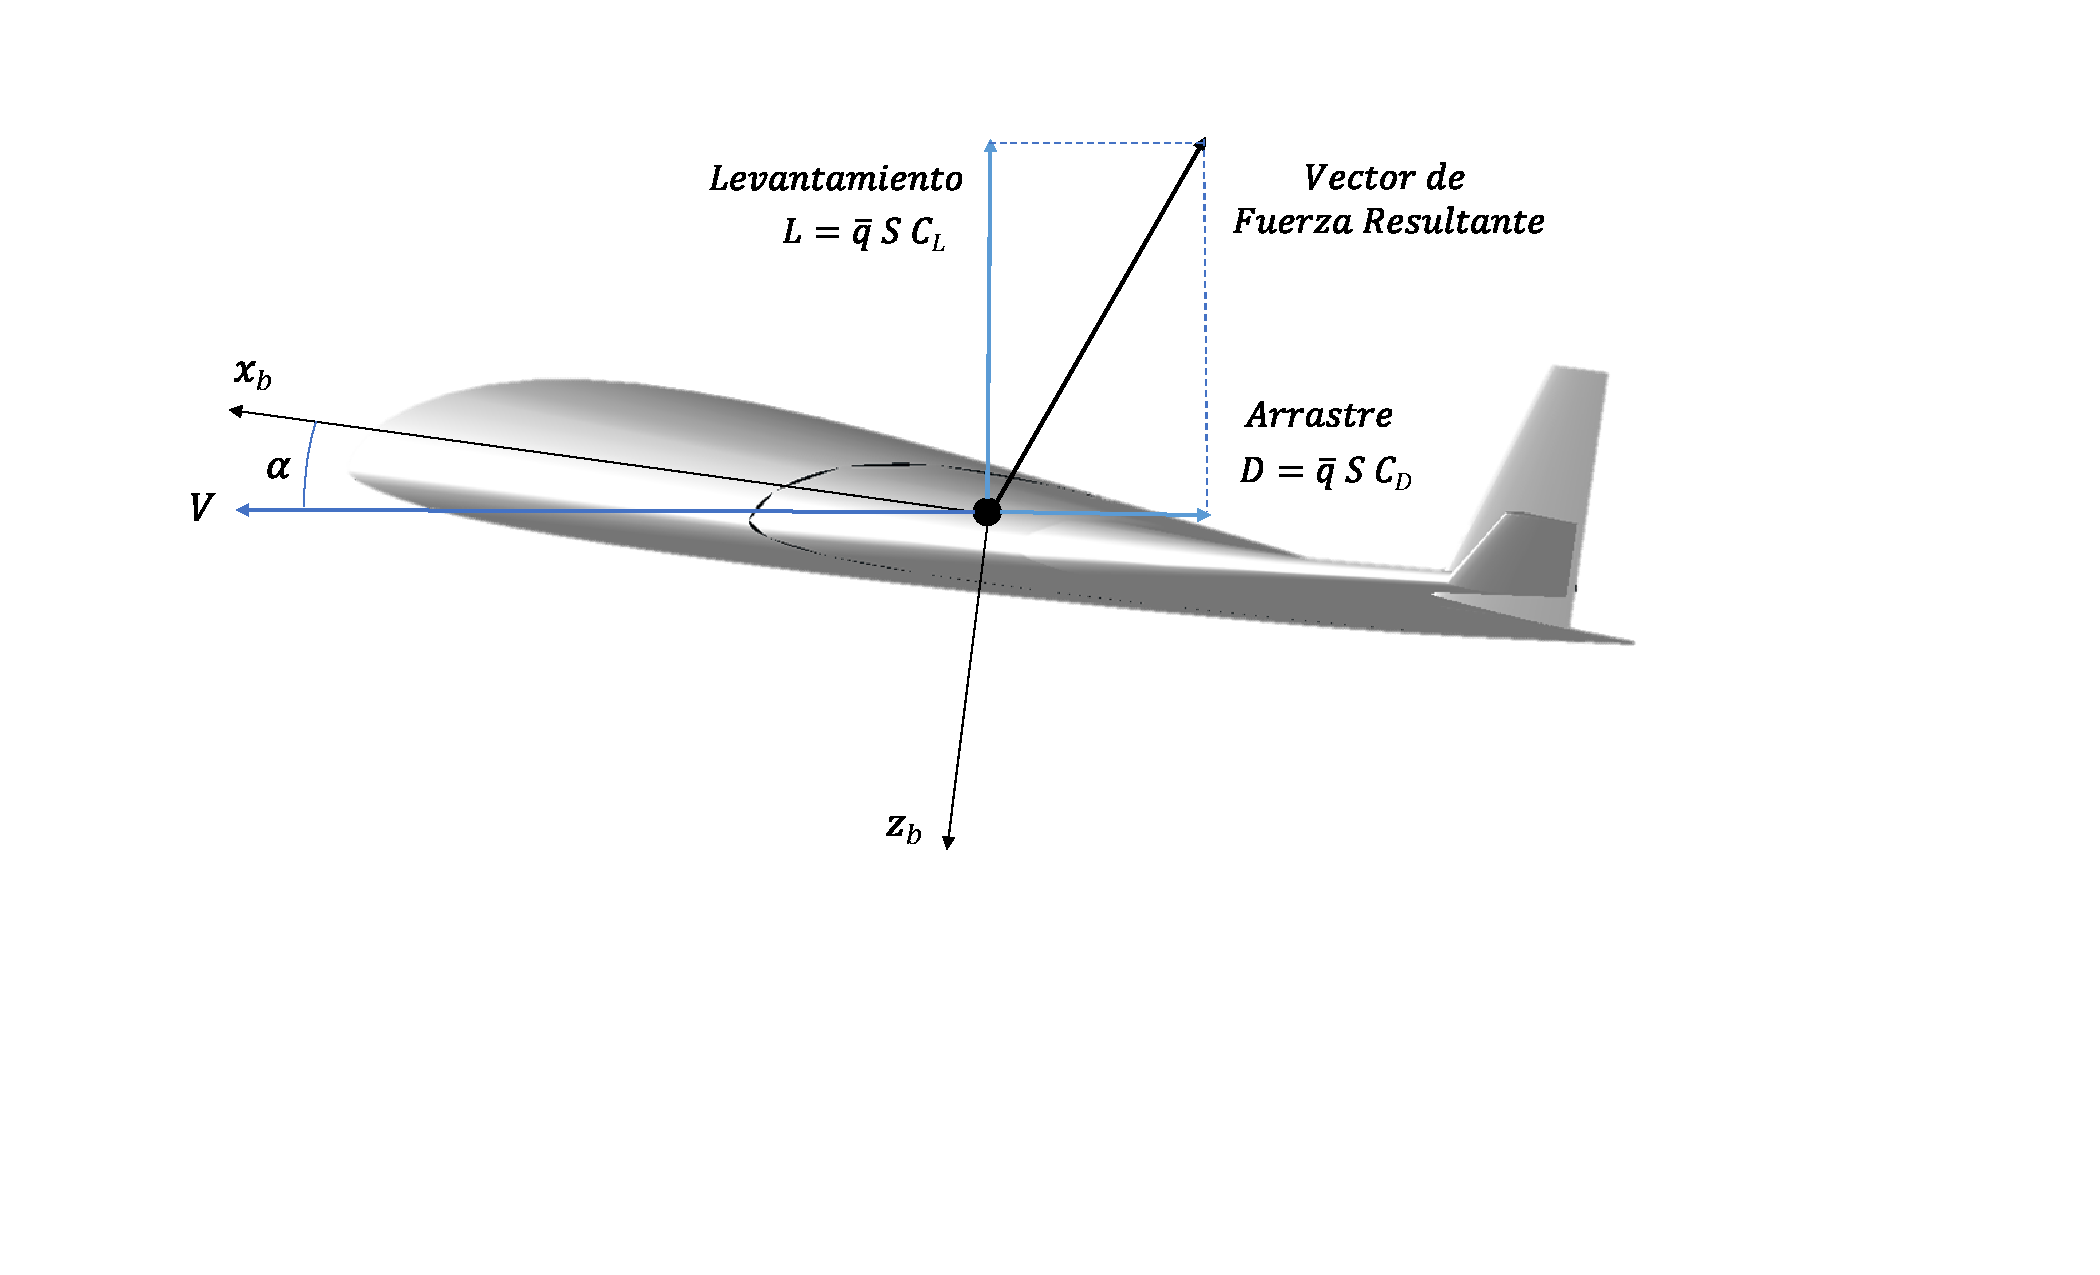
\includegraphics[scale=0.47]{Capitulo3/figs/fuerzas aerodinamicas_cropped.pdf}
\caption{Componentes de fuerza de la aeronave durante vuelo en equilibrio}
\label{fig: fuerzas aerodinamicas}
\end{figure}

Las fuerzas $X,Z$ son orientadas cuando se genera al ángulo de ataque respecto al plano de referencia a nivel de vuelo o plano de simetría $x-z$.
Las fuerzas de levantamiento y arrastre se combinan en una fuerza resultante, que puede ser considerada como un vector descrito por las componentes de tal sistema de coordenadas, es decir, los componentes de las fuerzas X y Z pueden ser expresados en términos de L y D por las siguientes ecuaciones: 

\begin{align}\
X = -D C_{\alpha}+LS_{\alpha}\\
Z = -D S_{\alpha} - LC_{\alpha}
\end{align}


En notación matricial:


\begin{gather} 
\begin{bmatrix}
X\\
Z
\end{bmatrix}
=
\begin{bmatrix}
-C_{\alpha} & S_{\alpha}\\ 
-S_{\alpha} & -C_{\alpha}
\end{bmatrix}
\begin{bmatrix}
 D\\
L
\end{bmatrix}
=
T_{\alpha}
\begin{bmatrix}
D \\
L
\end{bmatrix}
\end{gather}

donde $T_{\alpha}$ representa la matriz de transformación angular rotacional de $\alpha$.

\medskip

Ahora consideremos la dirección inversa resolviendo la transformación de las coordenadas de las fuerzas aerodinámicas respecto a los ejes cuerpo de la aeronave. 


\begin{gather} 
\begin{bmatrix}
D\\
L
\end{bmatrix}
=
\begin{bmatrix}
-C_{\alpha} & -S_{\alpha}\\ 
S_{\alpha} & -C_{\alpha}
\end{bmatrix}
\begin{bmatrix}
X\\
Z
\end{bmatrix}
=
T_{\alpha}^{-1}
\begin{bmatrix}
X \\
Z
\end{bmatrix}
\end{gather}

Entonces, uno puede notar que la matriz inversa es igual a la transpuesta de la matriz original $T_{\alpha}^{-1}=T_{\alpha}^T$, y por definición: es una matriz ortogonal; dado que su transpuesta es igual a su inversa.
%
Al generarse el ángulo $\alpha$, podemos expresar $X,Z$ a partir del sistema de coordenadas  $L,D$. 

\medskip

%%%%%%%%%%%%%%%%%%
\section{Dinámica}
La dinámica estudia las causas que originan el movimiento de los cuerpos. En esta sección se desarrollan las seis ecuaciones de movimiento (seis grados de libertad) de la aeronave considerando las fuerzas lineales y angulares que generan el movimiento.

 La segunda ley de Newton establece que la suma de fuerzas externas que actúan sobre un cuerpo en un sistema de referencia inercial es igual a la razón de cambio en el tiempo de acuerdo con su momento angular y lineal. 

 Las ecuaciones de la mecánica de vuelo de la aeronave basadas en la conservación del momento angular y lineal, se desarrollan basándonos principalmente en los desarrollos mencionados en \cite{Schimdt1998} y \cite{USAF1988}.

 \begin{figure}[!h]
\centering
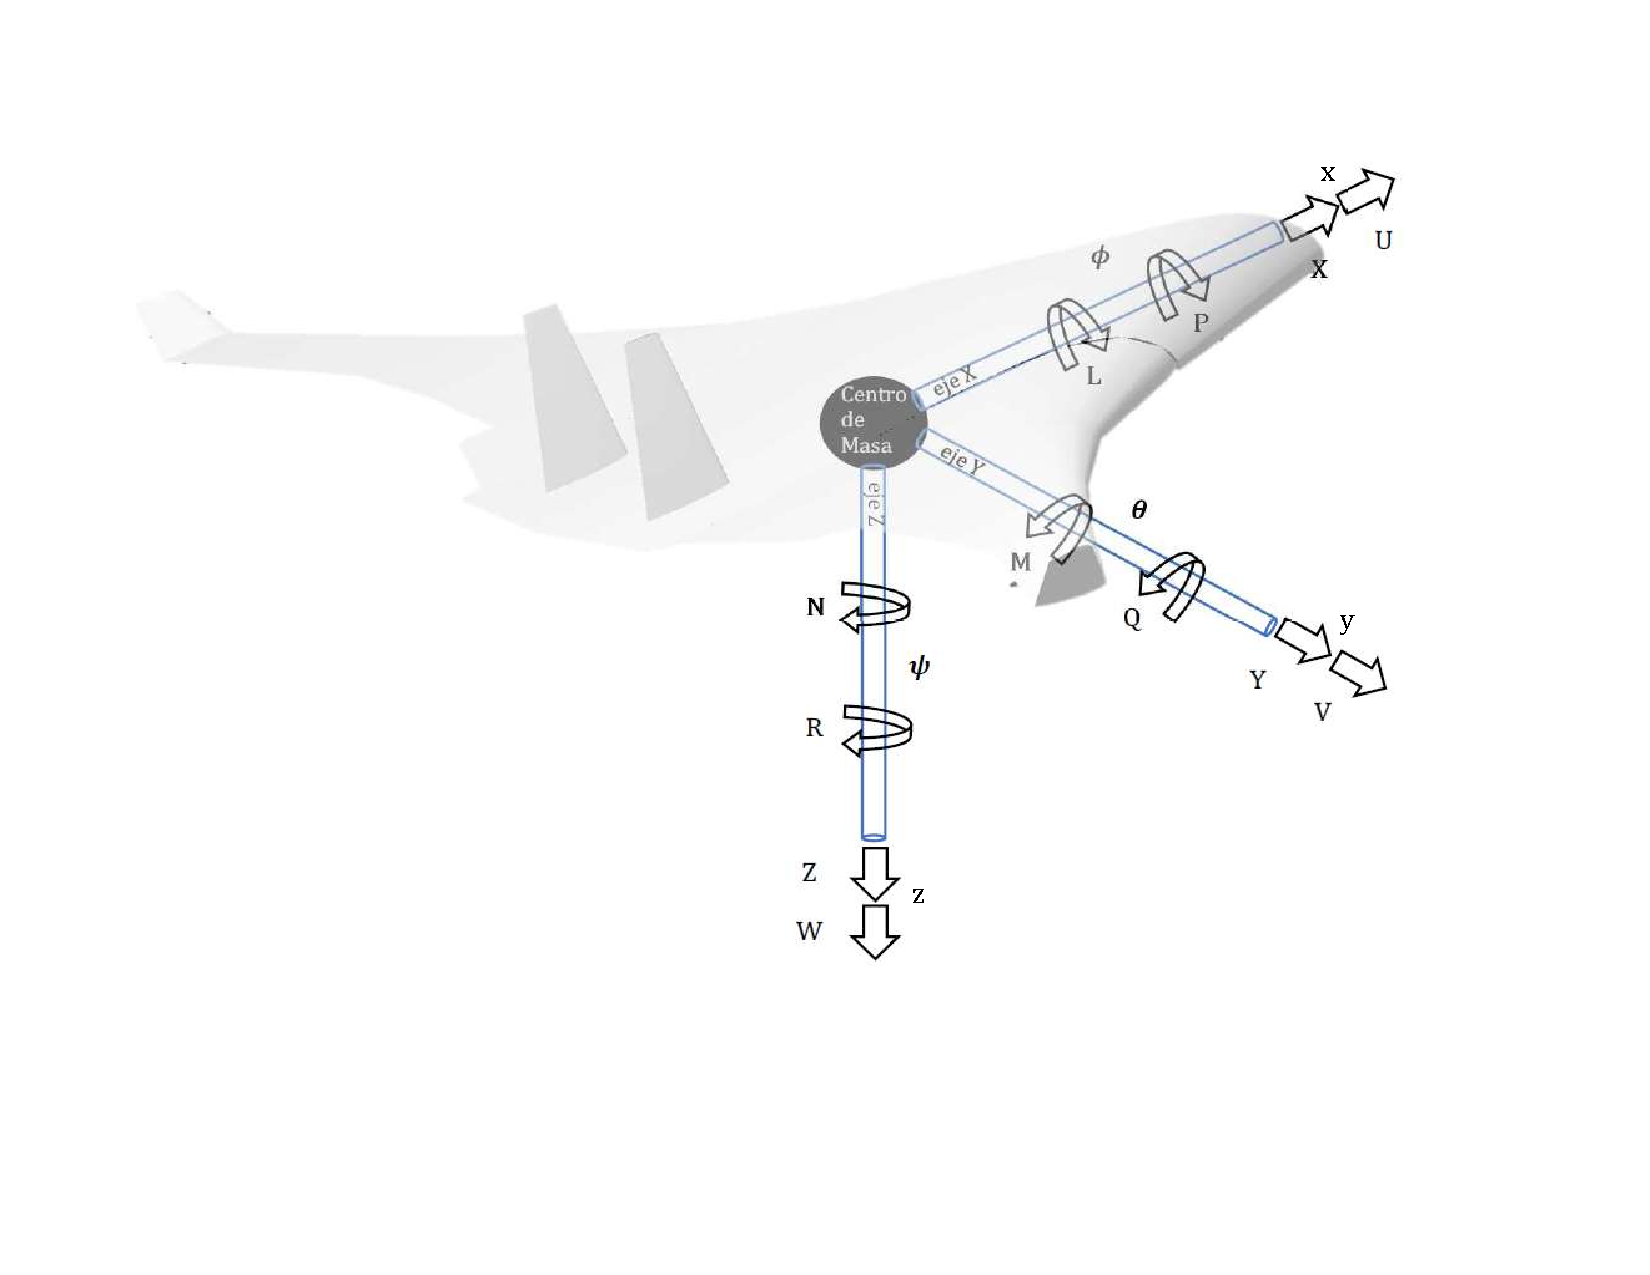
\includegraphics[scale=0.57]{Capitulo3/figs/dinamica ehekatl_cropped.pdf}
\caption{Posición, velocidad, fuerzas y momentos aplicados en ejes cuerpo}
\label{fig: posicion, velocidad, fuerzas y momentos}
\end{figure}
%
\begin{table}[!h]
\caption{Variables dinámicas en los ejes cuerpo de la aeronave}
\centering
\begin{tabular}{|r|r|r|r|}
     \hline
    \textbf{Dinámica de aeronave} & eje x & eje y & eje z \\
     \hline
     Momento angular & L & M & N \\
     \hline
     Velocidad angular & p & q & r \\
     \hline
     Posición angular & $\phi$ & $\theta$ & $\psi$ \\
     \hline
     Fuerza lineal & X & Y & Z \\
     \hline
     Velocidad lineal & u & v & w \\
     \hline
     Posición lineal & x & y & z \\
     \hline
\end{tabular}
\label{tab: variables dinamicas}
\end{table}
 
En la Figura \ref{fig: posicion, velocidad, fuerzas y momentos} tenemos la representación general de las fuerzas y momentos que actúan como componente en cada eje cuerpo de las aeronave (eje x, eje y, eje z). Tenemos 6 grados de libertad, un grado de libertad lineal y angular por cada eje.  

En la tabla \ref{tab: variables dinamicas} se definen las variables consideradas en la Figura \ref{fig: posicion, velocidad, fuerzas y momentos}.

\medskip

\textbf{Momento Lineal Traslacional}\\
La segunda ley de Newton define el movimiento traslacional como
\begin{equation}
\bar{F} = \frac{d}{dt}(m \bar{V})
\end{equation}
dónde $\bar{F}$ es la suma de las fuerzas lineales externas aplicadas y $m \bar{V}$ es el momento lineal.
$\bar{F}$ es un vector que puede representarse en ecuaciones traslacionales de 3 grados de libertad (de acuerdo con cada componente del espacio tridimensional).

El vector de fuerzas externas se define como la suma de todas las fuerzas aplicadas en la aeronave $\bar{F}=F_{Aero}+F_{Gravedad}+F_{Propulsion}+F_{Control}+F_{Perturbaciones}$. Los términos mencionados se desarrollan propiamente en la sección de \textit{fuerzas y momentos aplicados}.

\begin{table}[!h]
\caption{Fuerzas y momentos aplicados en la aeronave}
\centering
\begin{tabular}{|r|r|r|r|r|r|}
     \hline
     $\bar{F}/\bar{G}$ & Aerodinámica & Gravedad & Propulsión & Control & Perturbaciones \\
     \hline
     \textbf{X} & $X_{A}$ & $X_{G}$ & $X_{T}$ & $X_{C}$ & $X_{P}$ \\
     \hline
     \textbf{Y} & $Y_{A}$ & $Y_{G}$ & $Y_{T}$ & $Y_{C}$ & $Y_{P}$ \\
     \hline
     \textbf{Z} & $Z_{A}$ & $Y_{G}$ & $Y_{T}$ & $Z_{C}$ & $Z_{P}$ \\
     \hline
     \textbf{L} & $L_{A}$ & 0 & 0 & $L_{C}$ & $L_{P}$ \\
     \hline
     \textbf{M} & $M_{A}$ & 0 & 0 & $M_{C}$ & $M_{P}$ \\
     \hline
      \textbf{N} & $N_{A}$ & 0 & 0 & $N_{C}$ & $N_{P}$ \\
     \hline
\end{tabular}
\end{table}

La velocidad en el sistema de referencia inercial fijo de ejes terrestres respecto al sistema de referencia de ejes cuerpo de la aeronave se representa como

\begin{equation}
\label{momento lineal traslacional}
    F = m ( \frac{d \bar{V}}{dt}\mid_{x_{T} y_{T} z_{T}}) = m (\frac{d \bar{V}}{dt}\mid_{x_{B} y_{B} z_{B}} + \bar{\omega} \times \bar{V} )
\end{equation}

dónde se asume una masa $m$ constante. $\bar{V}$ y $\bar{\omega}$ son los vectores para las velocidades lineales $u,v,w$ y angulares $p,q,r$, respectivamente. Es decir,

\begin{equation}
    \bar{V} = u\bar{i}+v\bar{j}+w\bar{k} 
\end{equation}

\begin{equation}
    \bar{\omega} = p\bar{i}+q\bar{j}+r\bar{k} 
\end{equation}


En la dinámica de vuelo tenemos cuatro vectores para las ecuaciones de movimiento de la aeronave ($\bar{V}, \bar{\omega}, \bar{F}, \bar{G}$), dónde $\bar{F}$ y $\bar{G}$ son las fuerzas y momentos externos aplicados que desarrollaremos más adelante. 

\medskip

Desarrollando la ecuación (\ref{momento lineal traslacional}) en sus componentes obtenemos

\begin{equation}
    \bar{F} = m(\dot{u}\bar{i}+\dot{v}\bar{j}+\dot{w}\bar{k}+\begin{bmatrix}
    \bar{i} & \bar{j} & \bar{k} \\
    p & q & r \\
    u & v & w
    \end{bmatrix}) 
\end{equation}


\begin{equation}
    \bar{F} = m(\dot{u}\bar{i}+\dot{v}\bar{j}+\dot{w}\bar{k}+
    (qw-rv)\bar{i} + (pw-ru)\bar{j} + (pv-qu)\bar{k}) 
\end{equation}

\begin{equation}
    \bar{F} = m((\dot{u}+qw-rv)\bar{i} + (\dot{v}+pw-ru)\bar{j} + (\dot{w}+pv-qu)\bar{k}) 
\end{equation}

Finalmente se definen las ecuaciones del momento lineal traslacional en sus componentes tridimensionales

\begin{gather}
\label{eq: momento lineal}
    \bar{F} = F_x \bar{i} + F_y \bar{j} + F_z \bar{k} = X + Y + Z 
\end{gather}

dónde

\begin{gather}
\label{eq dinam tras 1}
    X = m(\dot{u} + qw - rv) \\
    Y = m(\dot{v} + ru - pw) \\
    Z = m(\dot{w} + pv - qu)
\label{eq dinam tras 2}
\end{gather}


\medskip
%%%%%%%%%%%%%%%%%%%%%%%%%%%%%%%%%%%%%%%%%%%%%%%%%%%%%%%%%%%%%%%%%%%%%%%%%%%%%
\textbf{Momento Angular Rotacional}\\
De la misma manera en que el vector de fuerzas externas $\bar{F}$ cambia el momento lineal ($\bar{F}=\frac{d}{dt}m\bar{V}$), los momentos externos $\bar{G}$ cambian el momento angular ($\bar{G}=\frac{d}{dt}\bar{H}$).

La segunda ley de Newton define el movimiento rotacional

\begin{equation}
\label{eq: movimiento rotacional}
\bar{G} = \frac{d}{dt}(\bar{H})
\end{equation}

dónde $\bar{G}$ es la suma de los momentos externos aplicados $\bar{G}=G_{Aero}+G_{Propulsion}+G_{Control}+G_{Perturbaciones}$ y $\bar{H}$ es el momento angular aplicado. 
$\bar{G}$ es un vector que puede representarse en tres ecuaciones rotacionales de 3 grados de libertad (de acuerdo con cada componente del espacio tridimensional). 
Podemos entender el momento angular como un momento lineal con brazo de palanca incluido. 

\begin{gather}
    \bar{P} = m\bar{V} \\
    \bar{H} = \bar{r} \times \bar{P}
\end{gather}

dónde $\bar{P}$ es el momento lineal y  $\bar{r}$ es el brazo de palanca. El ángulo entre $\bar{r}$ y $\bar{V}$ es de 90° y la magnitud del momento angular es de $mrV$. 

Definidos los productos y momentos de inercia, se establece la ecuación del momento angular de un cuerpo rígido 

\begin{equation}
    \bar{H} = H_x \bar{i} + H_y \bar{j} + H_z \bar{k}
\end{equation}

Entonces

\begin{gather}
    H_x = p I_{x} - q I_{xy} - r I_{xz} \\
    H_y = q I_{y} - r I_{yz} - p I_{xy} \\
    H_z = r I_{z} - p I_{xz} - q I_{yz}
\end{gather}

%% Define the equations of an airplane which is completely asymmetric
%% Then explain what the plane of symmetry is, and reduce the equations

Considerando que los ejes cuerpo x-z están en el plano de simetría de la aeronave, podemos reducir dos productos de inercia, tal que $I_{xy} = I_{yz} = 0$. 
Con esta consideración la ecuación del momento angular de una aeronave simétrica se simplifica

\begin{equation}
    \bar{H} = (p I_{x} - r I_{xz})\bar{i} + q I_{y}\bar{j} + (r I_{z} - p I_{xz})\bar{k} 
\end{equation}

Y recordando la ecuación (\ref{eq: movimiento rotacional}) podemos expresarla de acuerdo con el sistema inercial de los ejes terrestres. 

\begin{equation}
    \bar{G} = \frac{d\bar{H}}{dt} | x_T y_T z_T
\end{equation}

Expresando en los ejes cuerpo de la aeronave 

\begin{equation}
    \bar{G} = \frac{d\bar{H}}{dt} | x_B y_B z_B + \bar{\omega} \times \bar{H}
\end{equation}

Desarrollando, tenemos que

\begin{equation}
    \bar{G} = \dot{H}_{x} \bar{i} + \dot{H}_{y} \bar{j} + \dot{H}_{z} \bar{k} + \begin{bmatrix}
    \bar{i} & \bar{j} & \bar{k} \\
    p & q & r \\
    H_{x} & H_{y} & H_{z}
    \end{bmatrix}
\end{equation}

Dado que el cuerpo de la aeronave se asume como un cuerpo rígido, los momentos y productos de inercia son constantes. 

\begin{equation}
    \bar{G} = (\dot{p} I_{x} - \dot{r} I_{xz})\bar{i} + \dot{q} I_{y}\bar{j} + (\dot{r} I_{z} - \dot{p} I_{xz})\bar{k} + \begin{bmatrix}
    \bar{i} & \bar{j} & \bar{k} \\
    p & q & r \\
    (p I_{x} - r I_{xz}) & q I_{y} & (r I_{z} - p I_{xz})
    \end{bmatrix} 
\end{equation}

Por tanto, los componentes rotacionales tridimensionales son

\begin{gather}
\label{eq: momento angular 1}
    G_x = \dot{p} I_{x} + qr (I_{z} - I_{y}) - (\dot{r} + pq) I_{xz} \\
    G_y = \dot{q} I_{y} - pr (I_{z} - I_{x}) + (p^2 - r^2) I_{xz} \\
    G_z = \dot{r} I_{z} + pq (I_{y} - I_{x}) + (qr - \dot{p}) I_{xz}
\label{eq: momento angular 2}
\end{gather}

Y con esto tenemos completo el conjunto de ecuaciones rotacionales.
En la siguiente sección se desarrollan las fuerzas y momentos aplicados, $\bar{F}$ y $\bar{G}$. 

\bigskip
%%%%%%%%%%%%%%%%%%%%%%%%%%%%%%%%%%%%%%%%%%%%%%%%%%%%%%%%%%%%%%%%%%%%%%
\section{Fuerzas y Momentos Aplicados}

Las fuerzas y momentos aplicados en la aeronave son igual a la sumatoria de los términos de las fuerzas: aerodinámicas $_A$, de gravedad  $_G$, de propulsión  $_T$, de control  $_C$ y de perturbaciones atmosféricas $_P$. 
De acuerdo con las ecuaciones de conservación lineal \ref{eq dinam tras 1}-\ref{eq dinam tras 2} y conservación angular \ref{eq: momento angular 1}-\ref{eq: momento angular 1} se puede definir



\begin{align}
    X_{A} + X_{G} + X_{T} + X_{C} + X_{P} &= m (\dot u + qw - rv) \\
    Y_{A} + Y_{G} + Y_{T} + Y_{C} + Y_{P} &= m (\dot v + ru - pw) \\
    Z_{A} + Z_{G} + Z_{T} + Z_{C} + Z_{P} &= m (\dot w + pv - qu) \\
    L_{A} + L_{T} + L_{C} + L_{P} &= \dot p I_{x} + qr(I_{z} - I_{y}) - (\dot r + pq)I_{xz} \\
    M_{A} + M_{T} + M_{C} + M_{P}  &= \dot q I_{y} + pr(I_{z} - I_{x}) + (p^2 - r^2)I_{xz} \\
    N_{A} + N_{T} + N_{C} + N_{P} &= \dot r I_{z} + pq(I_{y} - I_{z}) + (qr - \dot p)I_{xz}
\end{align}


%%%%%%%%%%%%%%%%%%%%%%%%%%%%%%%%%%%%%%%%%%%%%%%%%%%%%%%%%%%%%%%%%%%%%%%%%%%%%%%%%%%%%%%%%%%%
\textbf{Fuerza de Gravedad}


Asumiendo que la altitud de la aeronave es no significativa en comparación con el radio de la tierra, es suficiente considerar la magnitud de la gravedad como constante. 

El peso de la aeronave (fuerza gravitatoria) entrará en las ecuaciones de movimiento representado en una componente por cada eje cuerpo de la aeronave.
Consideramos el peso de la aeronave $W=mg$ en el plano de referencia inercial (plano horizonte local) dado que la fuerza gravitatoria se asume como una fuerza lineal y constante hacia el centro de la tierra.
En la figura \ref{fig: fuerza gravitacional} podemos observar la transformación del cuerpo de la aeronave, donde en su condición inicial, el eje $x_b$ es paralelo y coincidente al eje $x_h$, y después de un movimiento de cabeceo, el eje $x_b$ tiene cierta distancia angular del eje $x_h$.  
\begin{figure}[!h]
\centering
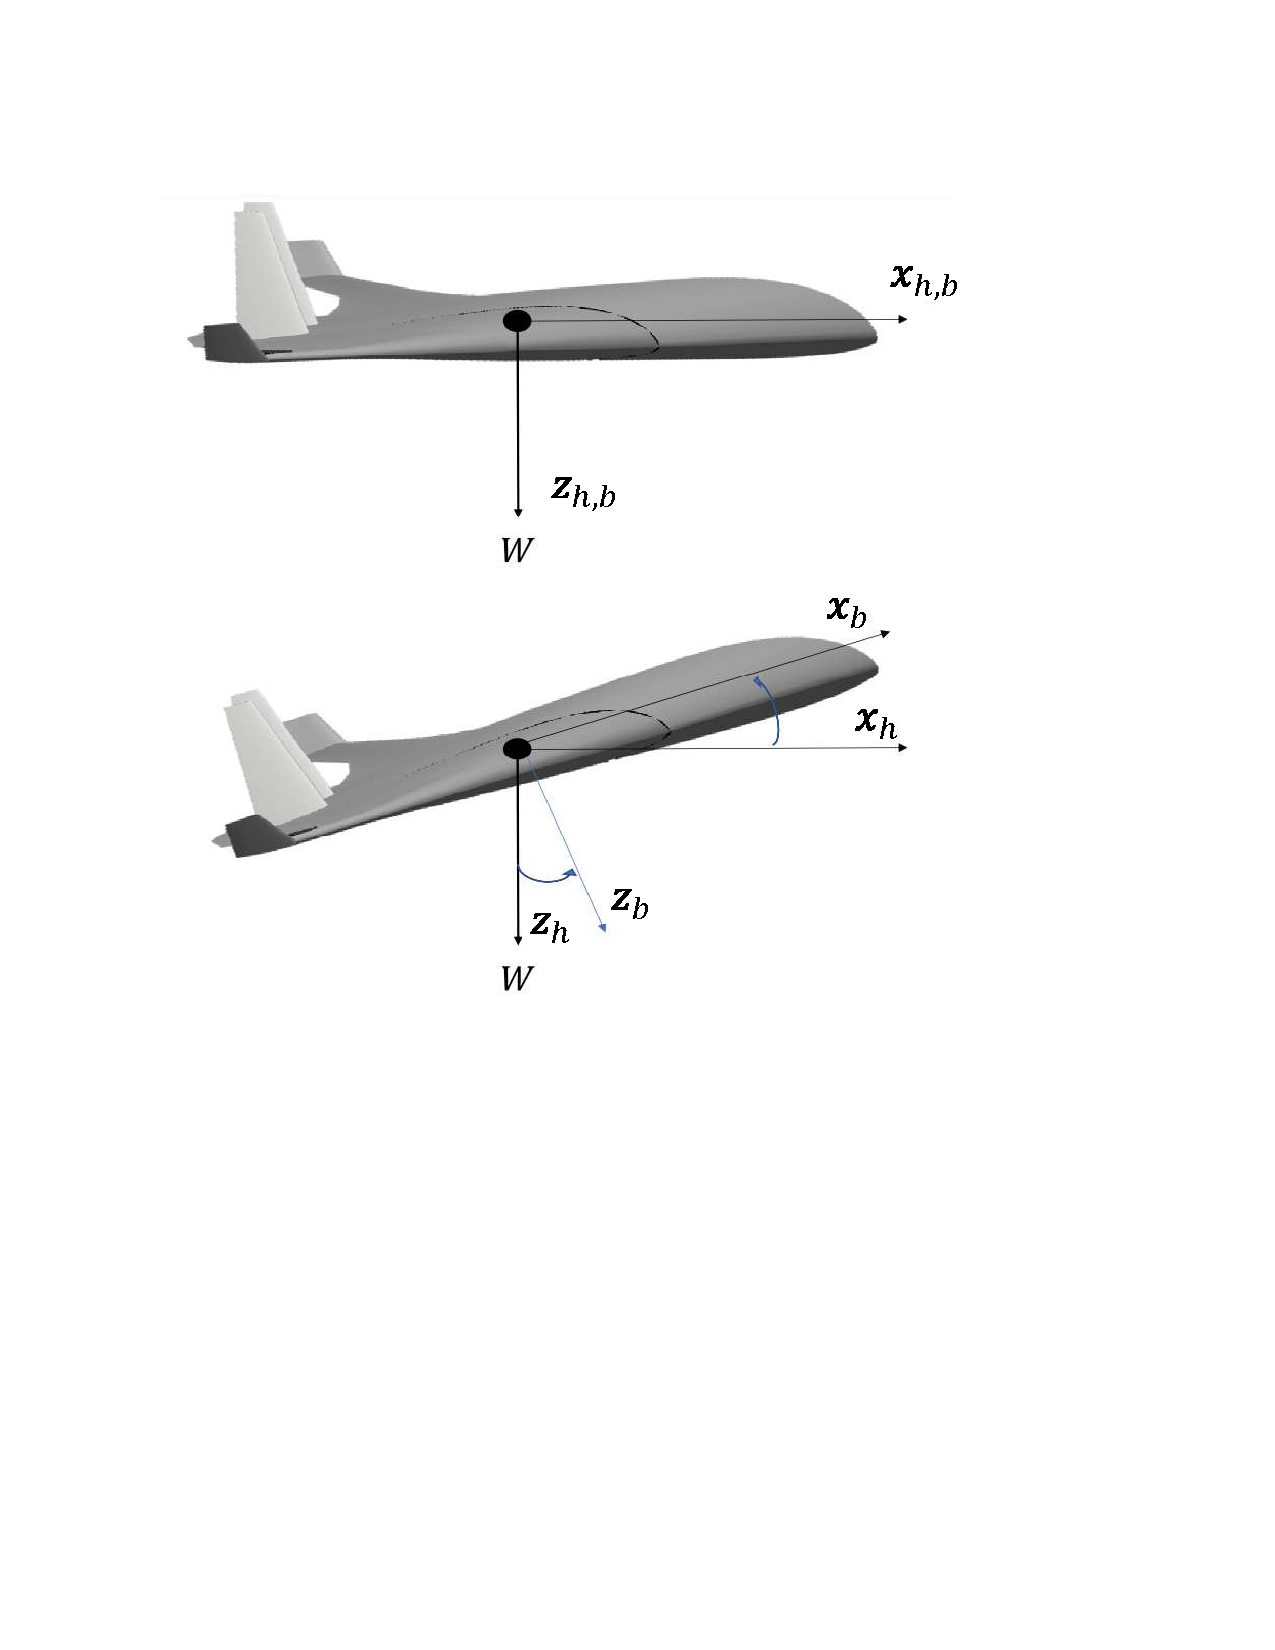
\includegraphics[scale=0.7]{Capitulo3/figs/peso gravedad_cropped (1).pdf}
\caption{Fuerza gravitacional en el  plano de horizonte local respecto al plano cuerpo de la aeronave}
\label{fig: fuerza gravitacional}
\end{figure}
En el plano horizonte local la fuerza gravitatoria queda representada en el siguiente vector
\begin{gather}
    W_{h}
    =
    \begin{bmatrix}
    0 & 0 & mg 
    \end{bmatrix}^T
\end{gather}
La componente del peso en los ejes cuerpo de la aeronave se encuentra utilizando la matriz de cosenos directores. Utilizar la transformación de la figura \ref{fig: fuerza gravitacional} es una referencia útil para obtenerla transformación del peso de la aeronave en el plano cuerpo a partir del plano horizonte local. 
%
Dado que asumimos los ejes cuerpo y su centro gravedad como el origen para las componentes de la gravedad, La contribución correspondiente al momento es cero $M_G = [0,0,0]^T$, y por tanto únicamente expresaremos la fuerza gravitacional en la sumatoria de fuerzas lineales. 

\begin{gather}
\label{gravedad ec}
    W_{b}
    =
    [S]
    \begin{bmatrix}
    0\\
    0\\
    mg
    \end{bmatrix}
    =
    (mg)
    \begin{bmatrix}
    -S_{\theta}\\
    C_{\theta} S_{\phi}\\
    C_{\theta} C_{\phi} 
    \end{bmatrix}
    =
    \begin{bmatrix}
    X_{G}\\
    Y_{G}\\
    Z_{G}
    \end{bmatrix}_{gravedad}
\end{gather}

por tanto

\begin{align}
    X_{G} &= - mg S_{\theta} \\
    Y_{G} &= mg  C_{\theta} S_{\phi}  \\
    Z_{G} &=  mg  C_{\theta} C_{\phi} 
\end{align}

En la ecuación \ref{gravedad ec} podemos apreciar que para obtener los componentes de la fuerza gravitacional en los ejes cuerpo de la aeronave se multiplica: la masa de la aeronave $m$ por la constante gravitacional $g$ por   la matriz de cosenos directores $[S]$.
La fuerza gravitacional es todo el tiempo paralela y su dirección coincidente con el eje z del plano horizonte local. 
En la figura \ref{fig: fuerza gravitacional} se muestra que aunque la orientación de los ejes cuerpo de la aeronave cambié, la dirección de la fuerza gravitacional sigue siendo constant en dirección del centro de gravedad hacia el centro de la tierra.
Dada esta naturaleza es que se aplica la matriz de cosenos directores para conservar estos valores respecto a los ejes cuerpo pese los cambios en actitud que puedan existir en la aeronave. 
Es importante reconocer que no todas las transformaciones de matrices son ortogonales, pero para el caso de la fuerza de gravedad, se puede aplicar esta transformación ortogonal. 

\bigskip
%%%%%%%%%%%%%%%%%%
\textbf{Fuerza de Propulsión}\\
Para vencer la inercia de una aeronave inmóvil, acelerarlo en la carrera de despegue, mantener una tasa de ascenso adecuada, alcanzar cierta velocidad en vuelo crucero o simplemente para vencer la resistencia al avance se necesita la fuerza de empuje o tracción. 
La reacción del empuje de los motores es de igual intensidad pero sentido opuesto (tercera ley de Newton) a la dirección hacia adelante que dirige a la aeronave. 
La dirección del empuje por convención suele considerarse de misma magnitud pero dirección contraria al eje cuerpo longitudinal de la aeronave, aunque en realidad, los motores suelen tener una pequeña desviación (1 o 2 grados Celsius regularmente, de eje longitudinal hacia abajo). 

\begin{figure}[h]
    \centering
    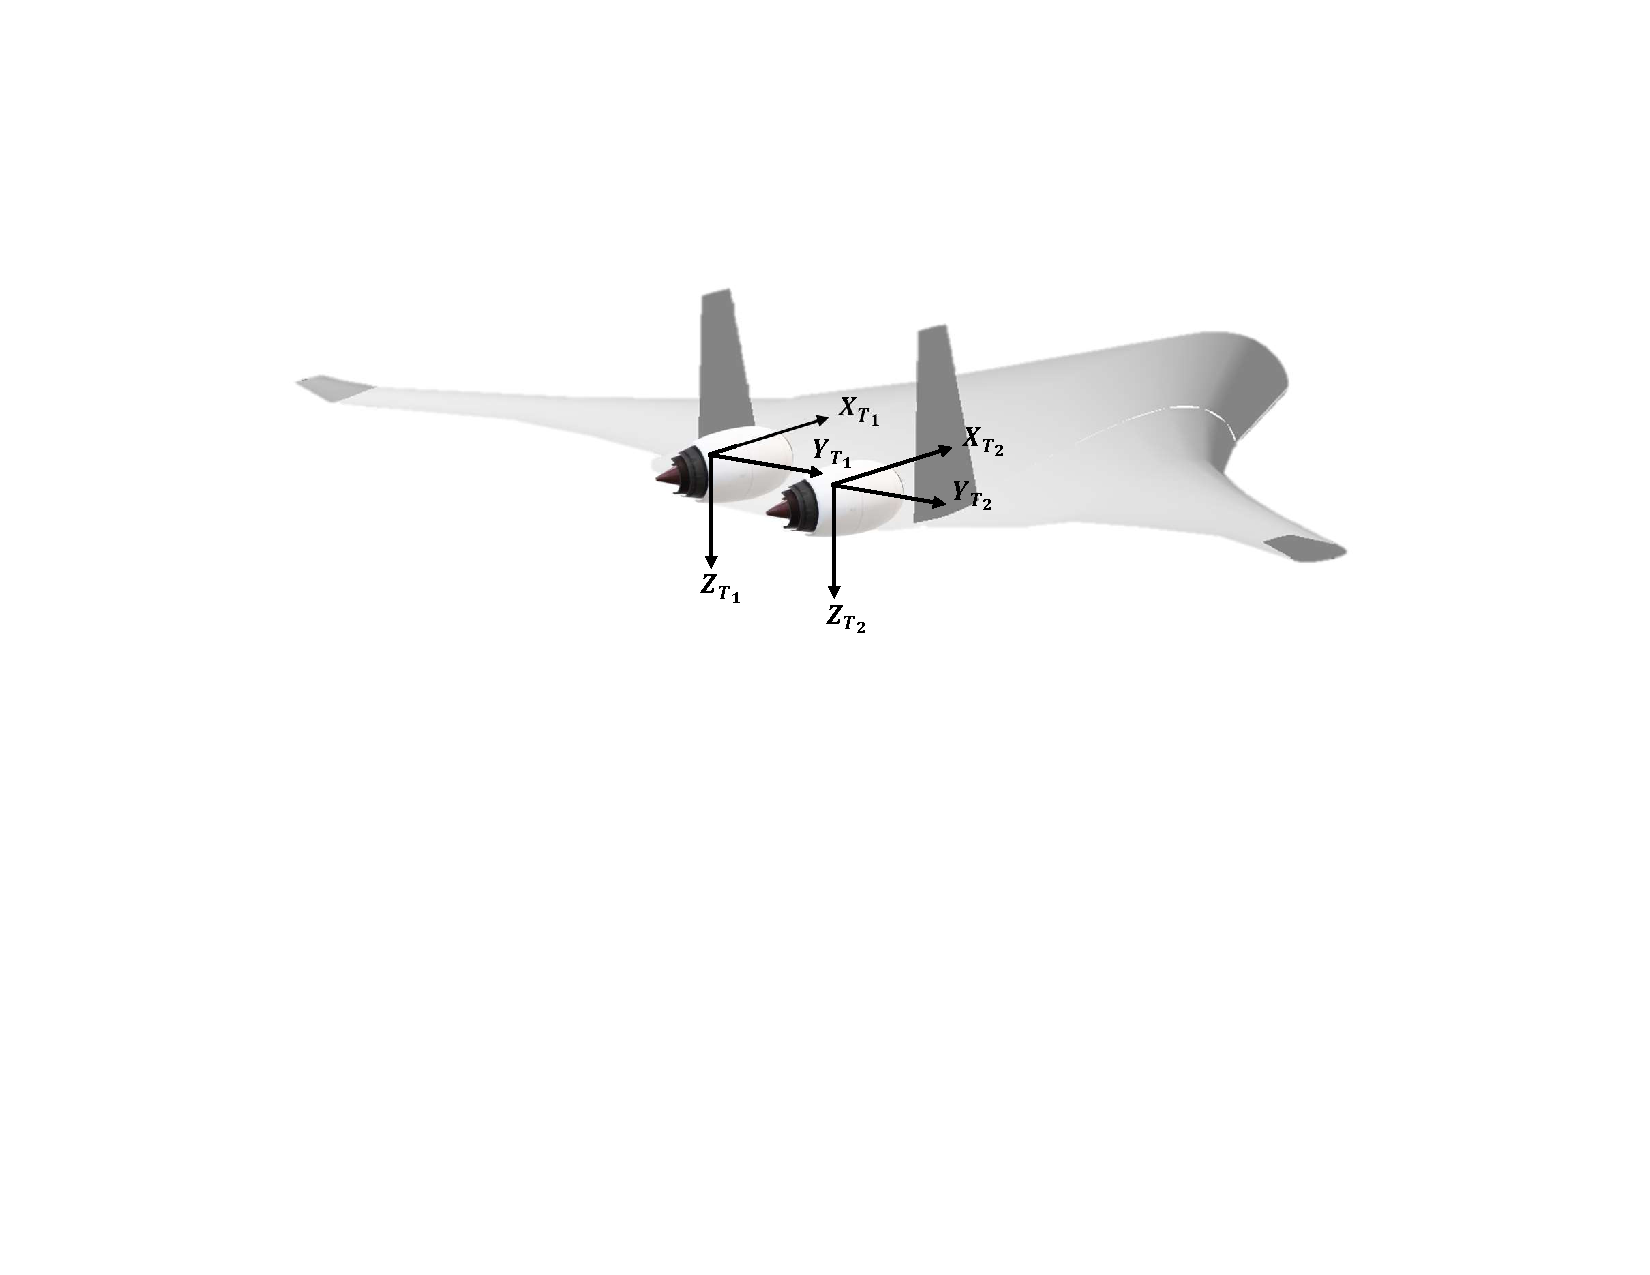
\includegraphics[scale=0.6]{Capitulo3/figs/motores 2_cropped.pdf}
    \caption{Fuerza de empuje}
    \label{Fuerza de empuje}
\end{figure}

La fórmula para determinar la fuerza de empuje se define como
\begin{equation}
    P_T = k_T T_{max}
\end{equation}

dónde\\
$T_{max}$ es el empuje máximo capaz de producir el motor(es). \\
$k_T$ es el coeficiente que índica el porcentaje de potencia del motor respecto a su capacidad máxima.

En EHEKATL BWB tenemos dos motores $T_1 , T_2$. De acuerdo con \cite{USAF1988}, las ecuaciones que describen el comportamiento de los motores en cada eje cuerpo de la aeronave respecto al plano de horizonte local son

\begin{align}
\label{eq motor 1}
    X_{T} &= P_{T1} C_{\theta} C_{\psi} + P_{T2} C_{\theta} C_{\psi} \\
    Y_{T} &= P_{T1}  S_{\psi} + P_{T2}  S_{\psi}  \\
    Z_{T} &= P_{T1}  C_{\psi} S_{\theta} + P_{T2}  C_{\psi} S_{\theta} 
\label{eq motor 2}
\end{align}

\bigskip
%%%%%%%%%%%%%%%%%%%%%%%%%%%%%%%%%%%%%%%%%%%%%%%%%%%%%%%%%%%%%%%%
\textbf{Fuerzas Aerodinámicas en la Aeronave}\\
Dos mecanismos físicos contribuyen para producir una fuerza aerodinámica. 
Primero, cada elemento de la superficie de área, multiplicado por la presión respecto a su posición, resulta en un elemento de fuerza normal de la superficie del perfil aerodinámico.
Segundo, por cada elemento de área en la superficie hay una capa del fluido en contacto con la superficie que no se mueve respecto a la superficie. 
La fuerza de fricción de la piel será proporcional al área de superficie alar (área en contacto con el fluido). 
La combinación de la fuerza de presión y la fuerza de fricción de la piel es la fuerza aerodinámica resultante sobre superficie sustentadora \cite{Lewis2016}, ver Figura \ref{fig: sustentacion, arrastre y momento}. 
\begin{figure}[!h]
\centering
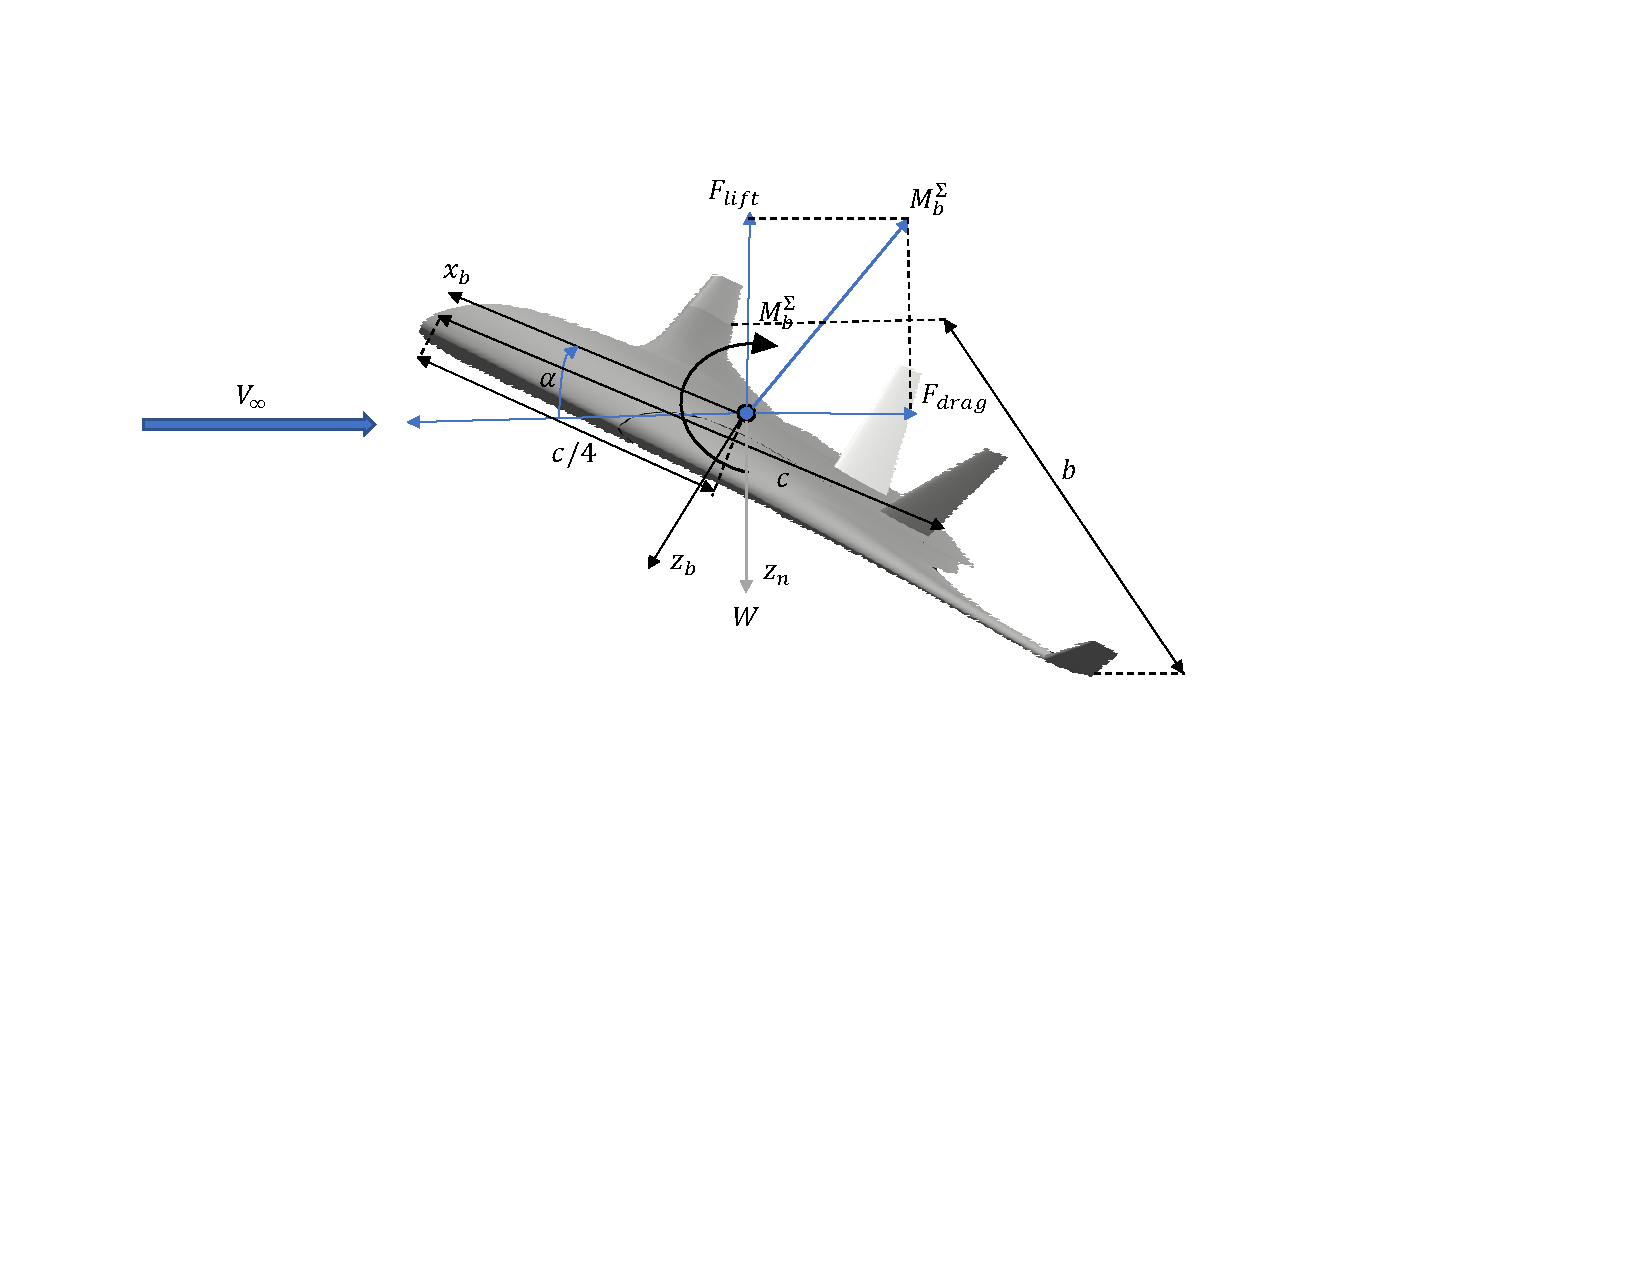
\includegraphics[scale=0.72]{Capitulo3/figs/Best Ehekatl_cropped.pdf}
\caption{Fuerzas de sustentación, arrastre y momento de cabeceo en el eje viento}
\label{fig: sustentacion, arrastre y momento}
\end{figure}
Los \textbf{coeficientes aerodinámicos adimensionales} describen el comportamiento aerodinámico de un perfil alar, ala (superficie sustentadora) o aeronave. Además, permiten la generalización de su desempeño dado que por el principio de similitud los resultados son constantes ante cualquier escala de mayor o menor proporción.
Los coeficientes aerodinámicos adimensionales se obtienen a través de simulaciones, pruebas en túnel de viento  y/o pruebas de vuelo en modelos a escala y tienen unidades de 1/rad o 1/degree. 
Los coeficientes aerodinámicos utilizados en este trabajo se definen como sumatoria de los coeficientes aerodinámicos no-dimensionales básicos, \cite{Mohammad2020}:
\begin{align}
\label{coeficientes adimensionales}
    C_{D} &= C_{D_{0}} + C_{D_{\alpha}} \alpha + C_{D_{q}}q\frac{c}{2U} + C_{D_{\dot \alpha}}\dot \alpha \frac{c}{2U} + C_{D_{u}} \frac{u}{U} + C_{D_{\delta_{e}}}\delta_{e} \\ 
    C_{Y} &= C_{Y_{\beta}}\beta + C_{Y_{p}}p\frac{b}{2U} + C_{Y_{r}}r \frac{b}{2U} + C_{Y_{\delta_{a}}}\delta_{a} + C_{Y_{\delta_{r}}}\delta_{r} \\
    C_{L} &= C_{L_{0}} + C_{L_{0}} \alpha + C_{L_{q}}q\frac{c}{2U} + C_{L_{\dot \alpha}}\dot \alpha \frac{c}{2U} + C_{L_{u}} \frac{u}{U} + C_{L_{\delta_{e}}}\delta_{e} \\
    C_{l} &= C_{l_{\beta}}\beta + C_{l_{p}}p\frac{b}{2U} + C_{l_{r}}r \frac{b}{2U} + C_{l_{\delta_{a}}}\delta_{a} + C_{l_{\delta_{r}}}\delta_{r} \\
    C_{m} &= C_{m_{0}} + C_{m_{\alpha}} \alpha + C_{m_{q}}q\frac{c}{2U} + C_{m_{\dot \alpha}}\dot \alpha \frac{c}{2U} + C_{m_{u}} \frac{u}{U} + C_{m_{\delta_{e}}}\delta_{e} \\
    C_{n} &= C_{n_{\beta}}\beta + C_{n_{p}}p\frac{b}{2U} + C_{n_{r}}r \frac{b}{2U} + C_{n_{\delta_{a}}}\delta_{a} + C_{n_{\delta_{r}}}\delta_{r}
\label{coeficientes adimensionales 2}
\end{align}

Los coeficientes aerodinámicos a-dimensionales en \ref{coeficientes adimensionales}-\ref{coeficientes adimensionales 2} contienen las \textbf{derivadas de estabilidad adimensionales}. $ C_{D_{q}}$ por ejemplo, describe cómo cambia la fuerza de arrastre $C_D$ en respuesta a la variable de movimiento de la tasa de giro de cabeceo $q$. La derivadas de estabilidad no-dimensionales son importantes para el diseño y la evaluación de la estabilidad y el control de una aeronave.

Los \textbf{coeficientes aerodinámicos dimensionales} son valores que describen el comportamiento aerodinámico de una aeronave. A diferencia de los coeficientes adimensionales, estos valores están expresados en unidades físicas y dependen de las dimensiones y características específicas de la aeronave.
En la Tabla \ref{Fuerzas y momentos aerodinámicos de la aeronave 2} se muestran los coeficientes aerodinámicos  dónde $\bar{q}$ es la \textbf{presión dinámica} que refiere a la energía cinética del flujo de aire por unidad de área.
\begin{equation}
    \bar{q} = \frac{1}{2} \rho V^2
\end{equation}
$S$ es el área de referencia de la superficie sustentadora, $b$ es la envergadura y $c$ es la cuerda raíz central.
\begin{table}[!h]
    \centering
    \begin{tabular}{|c|}
    \hline
    \textbf{Coeficientes Aerodinámicos de Estabilidad Dimensional}\\
    \hline
    $X_{A} = \bar{q} S C_{D} (\alpha, V_w, Mach, Re, u, w, q, \delta_e, \delta_T)$ \\
    $Y_{A} = \bar{q} S C_{Y} (\beta, V_w, Mach, Re, v, p, r, \delta_a , \delta_r, \delta_T)$  \\
    $Z_{A} = \bar{q} S C_{L} (\alpha, V_w, Mach, Re, u, w, q, \delta_T)$    \\
    $L_{A} = \bar{q} S b C_{l} (\beta,V_w, Mach, Re, v, p, r, \delta_a , \delta_r, \delta_T)$ \\
    $M_{A} = \bar{q} S c C_{m} (\alpha, V_w, Mach, Re, u, w, q, \delta_T)$  \\
    $N_{A} = \bar{q} S b C_{n} (\beta, V_w, Mach, Re, v, p, r, \delta_a , \delta_r, \delta_T)$  \\
    \hline
    \end{tabular}
    \caption{Fuerzas y momentos aerodinámicos de la aeronave}
    \label{Fuerzas y momentos aerodinámicos de la aeronave 2}
\end{table}


Las \textbf{derivadas de estabilidad dimensional} son medidas específicas de cómo las fuerzas y momentos aerodinámicos que actúan sobre una aeronave cambian en respuesta a perturbaciones en las condiciones de vuelo. Estas derivadas son cruciales para comprender la estabilidad y control de una aeronave en distintas situaciones.
Las derivadas de estabilidad longitudinal dimensional están relacionadas con el movimiento alrededor del eje lateral $y$, y describen como la aeronave responde a perturbaciones en el ángulo de ataque $\alpha$, la tasa de cabeceo $q$ y la tasa de variación de altura $\dot{w}$. Se encuentran en la Tabla \ref{tab:derivadas dimensionales longitudinales}, dónde $M$ es el número de Mach. 

\begin{table}[!h]
\begin{center}
\caption{Derivadas de Estabilidad dimensionales longitudinales \cite{Etkin1996}}
\begin{tabular}{| c | c | c | }
\hline
\multicolumn{3}{ |c| }{Derivadas de Estabilidad Longitudinal Dimensional} \\ 
\hline
$X_u$ & $ - \frac{ \bar{q} S}{mV}(2 C_{D} + M C_{D_{u}})$ & $s^1$ \\
$X_\alpha$ & $ - \frac{ \bar{q} S}{m} (C_L - C_{D_{\alpha}} )$ & $fts^-2 | ms^-2$\\
$X_q$ & $ - \frac{ \bar{q} S}{m} (\frac{c}{2V}  C_{D_{q}}$) & $fts^-2 | ms^-2$ \\ 
$Z_u$ & $ - \frac{ \bar{q} S}{m} (2C_L + M C_{L_{u}}) $ & $s^-1$\\
$Z_\alpha$ & $ - \frac{ \bar{q} S}{m} (C_D + C_{D_{\alpha}})$ & $fts^-2 | ms^-2$\\
$Z_q$ & $ - \frac{ \bar{q} S}{m} ( \frac{c}{2V}  C_{L_{q}} )$ & $fts^-1| ms^-1 $\\
$M_u$ & $ - \frac{ \bar{q} Sc}{I_y V}  (M  C_{m_{u}})$ & $ft^-1s^-1 | m^-1s^-1$\\
$M_\alpha$ & $ - \frac{ \bar{q} Sc}{I_y}  C_{m_{\alpha}}$ & $s^-2$\\
$M_q$ & $ - \frac{\bar{q} Sc}{I_y} (\frac{c}{2V} C_{m_{q}})$ & $s^-1$\\
\hline
\end{tabular}
\label{tab:derivadas dimensionales longitudinales}
\end{center}
\end{table}

Las derivadas de estabilidad lateral-direccional dimensional están relacionadas con el movimiento alrededor del eje longitudinal $x$ y eje normal $z$. Describen como la aeronave responde a perturbaciones en el ángulo de deslizamiento $\beta$, la tasa de alabeo $p$ y la tasa de guiñada $r$, ver Tabla \ref{tab:derivadas dimensionales laterales}.
\begin{table}[!h]
\begin{center}
\caption{Derivadas de estabilidad dimensionales lateral-direccional \cite{Etkin1996}}
\begin{tabular}{| c | c | c | }
\hline
\multicolumn{3}{ |c| }{Derivadas de Estabilidad Lateral-Direccional Dimensional} \\
\hline
$Y_\beta$ & $ - \frac{\bar{q} S}{m} C_{Y_\beta}$ & $fts^-2 | ms^-2$ \\
$Y_p$ & $ - \frac{ \bar{q} S}{m} (\frac{b}{2V}) C_{Y_p} $ & $fts^-1 | ms^-1$\\
$Y_r$ & $ - \frac{ \bar{q} S}{m} (\frac{b}{2V}) C_{Y_r} $ & $fts^-1 | ms^-1$ \\ 
$L_\beta$ & $ - \frac{ \bar{q}Sb}{I_x} C_{l_\beta} $ & $s^-2$\\
$L_p$ & $ - \frac{\bar{q}Sb}{I_x} (\frac{b}{2V}) C_{l_p} $ & $fts^-1 | ms^-1$\\
$L_r$ & $ - \frac{\bar{q}Sb}{I_x} (\frac{b}{2V}) C_{l_r}  $ & $s^-1$\\
$N_\beta$ & $ - \frac{\bar{q}Sb}{I_x} C_{n_\beta} $ & $s^-2$\\
$N_p$ & $ - \frac{\bar{q}Sb}{I_z} (\frac{b}{2V}) C_{n_p} $ & $s^-1$\\
$N_r$ & $ - \frac{\bar{q}Sb}{I_z} (\frac{b}{2V}) C_{n_r} $ & $s^-1$\\
\hline
\end{tabular}
\label{tab:derivadas dimensionales laterales}
\end{center}
\end{table}

La constante G está relacionada con la estabilidad lateral-direccional de la aeronave, la cual hace referencia a los momentos de inercia de la aeronave alrededor de los ejes principales de inercia: longitudinal $I_x$, lateral $I_y$ y vertical $I_z$.
\begin{equation}
    G = \frac{1}{[1 - (I_{xz})^2 / (I_x I_z)]}
\end{equation}
\begin{gather}
\label{ld dimensional 1}
    L_\beta ' = G [L_\beta + N_\beta (\frac{I_{xz}}{I_x})] \\
    L_p ' = G [L_p + N_p (\frac{I_{xz}}{I_x})] \\
    L_r ' = G [L_r + N_r (\frac{I_{xz}}{I_x})] \\
    N_\beta ' = G [N_\beta + L_\beta (\frac{I_{xz}}{I_x})] \\
    N_p ' = G [N_p + L_p (\frac{I_{xz}}{I_x})] \\
    N_r ' = G [N_r + L_r (\frac{I_{xz}}{I_x})] \\
\label{ld dimensional 2}
\end{gather}
Las derivadas de estabilidad mostras en \ref{ld dimensional 1}-\ref{ld dimensional 2} tienen en cuenta la estabilidad adicional G cuando hay perturbaciones. Ahora, comparemos $L_\beta$ con $L_\beta'$. la derivada  $L_\beta$ representa condiciones no perturbadas, mientras $L_\beta'$ considera la influencia de G y el acoplamiento lateral-direccional. 
En resumen, el término G en las derivadas de estabilidad lateral-direccional dimensionales introduce una corrección para tener en cuenta la influencia de los momentos de inercia en la estabilidad lateral-direccional de la aeronave. Estas derivadas son las que se utilizan para propósitos de simulación. 

\medskip

%%%%%%%%%%%%%%%%%%%%%%%%%%%%%%%%%%%%%%%%%%%%%%%%%%%%%%%%%
\textbf{Fuerzas de Control de Superficies Aerodinámicas}\\
La Figura \ref{fig: ACS in EHEKATL BWB} muestras las superficies de control aerodinámicas del modelo EHEKATL BWB, el cual cuenta con 8 elevons en el borde de fuga (cuatro por semi-ala) y dos timones direccionales (un par,uno por estabilizador vertical). 

\begin{figure}[!h]
\centering
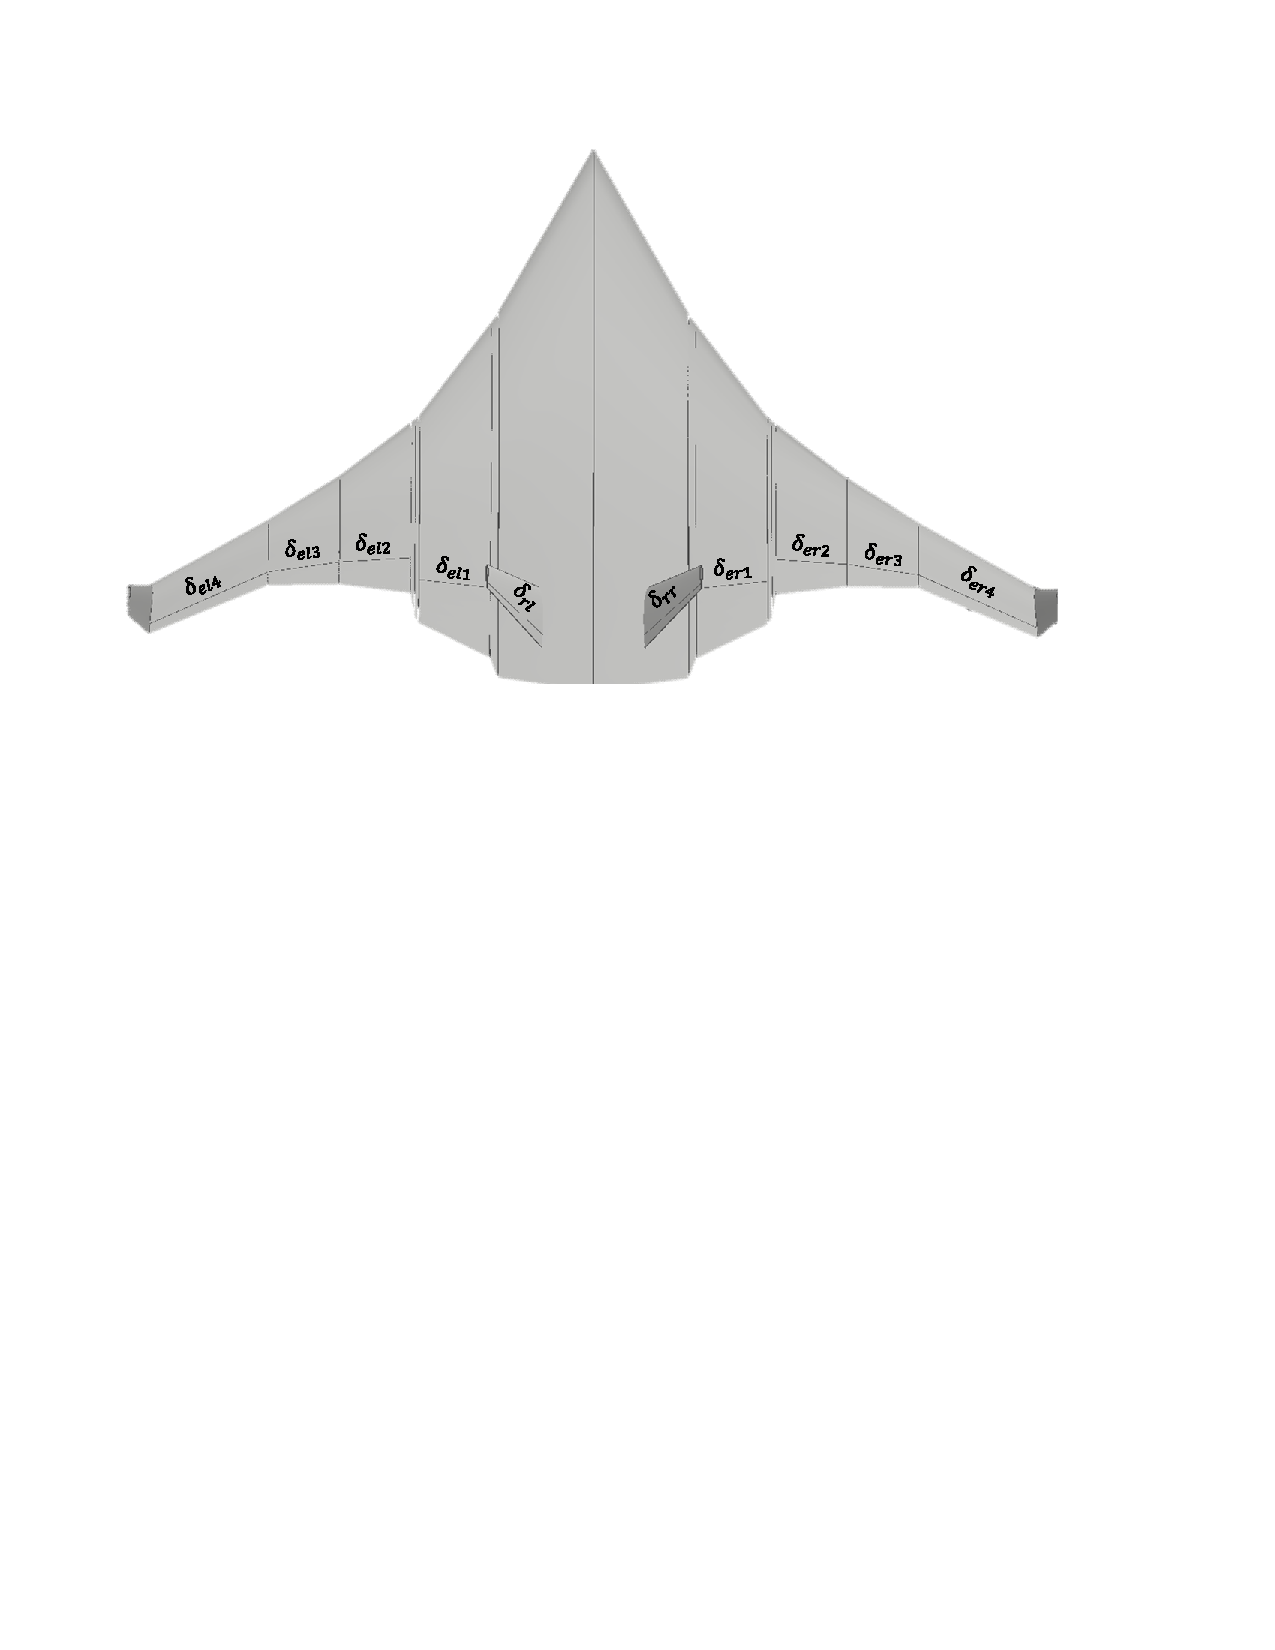
\includegraphics[scale=0.7]{Capitulo3/figs/ehekatl acs_cropped.pdf}
\caption{Superficies de control aerodinámicas en EHEKATL BWB}
\label{fig: ACS in EHEKATL BWB}
\end{figure}

Existen varias formas en que podemos configurar los  momentos generados por las ACS en el borde de fuga. 
Para una primera aproximación, y como base para el diseño de controladores para EHEKATL BWB, se establece la configuración de control convencional con entradas de control primarias: 
\begin{itemize}
    \item 2 pares de elevadores  ($\delta_{e1,e2}$)
    \item 2 pares de alerones  ($\delta_{e3,e4}$)
    \item 1 par de timón direccional  ($\delta_{r}$)
\end{itemize}

%\begin{table}[!h]
%    \centering
%    \begin{tabular}{|c|}
%    \hline
%    \textbf{Coeficientes Aerodinámicos de Control Dimensionales}\\
%    \hline
%     $X_{C} = \bar{q} S C_{D_{\delta_e}} (\alpha, V_w, Mach, Re, \delta_e, \delta_T)$  \\
%     $Y_{C} = \bar{q} S C_{Y_{\delta_a,\delta_r}} (\beta, V_w, Mach, Re, \delta_a , \delta_r, \delta_T)$  \\
%     $Z_{C} = \bar{q} S C_{L_{\delta_e}} (\alpha, V_w, Mach, Re, \delta_e, \delta_T)$   \\
%     $L_{C} = \bar{q} S b C_{l_{\delta_a,\delta_r}} (\beta, V_w, Mach, Re,\delta_a, \delta_r, \delta_T)$ \\
%     $M_{C} = \bar{q} S c C_{m_{\delta_e}} (\alpha, V_w, Mach, Re, \delta_e, \delta_T)$ \\
%    $N_{C} = \bar{q} S b C_{n_{\delta_a,\delta_r}} (\beta, V_w, Mach, Re, \delta_a , \delta_r, \delta_T)$ \\
%    \hline
%    \end{tabular}
%    \caption{Fuerzas y momentos aerodinámicos de la aeronave}
%    \label{Fuerzas y momentos aerodinámicos de la aeronave 3}
%\end{table}

En los coeficientes aerodinámicos a-dimensionales de la aeronave mostrados en \ref{coeficientes adimensionales}-\ref{coeficientes adimensionales 2} se observa la influencia de los coeficientes de control aerodinámicos a-dimensionales, que describen cómo cambian el momento aerodinámico en una aeronave como respuesta a las acciones de los control. $C_{m_{\delta_{}e}}$ por ejemplo, describe el comportamiento en el momento de cabeceo de la aeronave como respuesta al movimiento de deflexión de los elevadores $\delta_e$. 
%
Los coeficientes aerodinámicos de control dimensional relacionan los cambios en la posición o deflexión de las ACS de elevadores, alerones y timones de dirección con la respuesta en las fuerzas y momentos aerodinámicos de la aeronave, pero a diferencia de los coeficientes adimensionales, estos coeficientes proporcionan información considerando las dimensiones y características particulares de la aeronave.
Por un lado, las derivadas de control longitudinal dimensional se refieren a la respuesta del avión en la dinámica longitudinal cuando se aplican los elevadores. 
Mientras las derivadas de control lateral-direccional se refieren a la respuesta del avión en la dinámica lateral-direccional cuando se aplican los alerones y timones. 
La Tabla \ref{tab:derivadas control d} muestra las derivadas de control longitudinal y lateral-direccional dimensionales. 
\begin{table}[!h]
\begin{center}
\caption{Derivadas de Control Longitudinal Dimensional}
\begin{tabular}{| c | c | c | }
\hline
\multicolumn{3}{ |c| }{Derivadas de Control Longitudinal Dimensional} \\ 
\hline
$X_{\delta_e}$ & $ - \frac{\bar{q}S}{m} \frac{\partial C_D}{\partial \delta}$ & $fts^-2 | ms^-2$ \\
$Z_{\delta_e}$ & $ - \frac{\bar{q}S}{m}  \frac{\partial C_L}{\partial \delta}$ & $fts^-2 | ms^-2$ \\
$M_{\delta_e}$ & $ - \frac{\bar{q}Sc}{I_y}  \frac{\partial C_M}{\partial \delta}$ & $s^-2$\\
\hline
\hline
\multicolumn{3}{ |c| }{Derivadas de Control Lateral Dimensional} \\
\hline
$Y_{\delta_{a,r}}$ & $ - \frac{\bar{q}S}{m} \frac{\partial C_Y}{\partial \delta}$ & $fts^-2 | ms^-2$\\
$L_{\delta_{a,r}}$ & $ - \frac{\bar{q}Sb}{I_x}  \frac{\partial C_L}{\partial \delta}$ & $s^-2$\\
$N_{\delta_{a,r}}$ & $ - \frac{\bar{q}Sb}{I_z}  \frac{\partial C_n}{\partial \delta})$ & $s^-2$\\
\hline
\end{tabular}
\label{tab:derivadas control d}
\end{center}
\end{table}


Similar a las derivadas de estabilidad lateral-direccional, las derivadas de control lateral-direccional serán transformadas considerando la constante G para considerar las perturbaciones y el acoplamiento lateral-direccional de las ACS, ver ecuación \ref{eq control ld aaa}. 
\begin{gather}
\label{eq control ld aaa}
    L_{\delta_{a,r}} ' = G [L_\delta + N_\delta (\frac{I_{xz}}{I_x})] \\
    N_{\delta_{a,r}} ' = G [N_\delta + L_\delta (\frac{I_{xz}}{I_x})] \\
\end{gather}

%%%%%%%%%%%%%%%%%%%%%%%%%%%%%%%%%
\section{Modelo de EHEKATL BWB}

Finalmente, podemos establecer el conjunto de ecuaciones que gobiernan el movimiento de EHEKATL BWB de acuerdo con las ecuaciones \ref{vh 1} para cinemática traslacional, \ref{eq cinem rot} para cinemática rotacional, \ref{eq dinam tras 1}-\ref{eq dinam tras 2} para la dinámica traslacional y 
\ref{eq: momento angular 1}-\ref{eq: momento angular 2} para la dinámica rotacional. La ecuaciones mencionadas definen el modelo dinámico de vuelo acoplado de seis grados de libertad para EHEKATL BWB.

Los términos recalcados en azul son las entradas de control del sistema de acuerdo con la Tabla \ref{tab:derivadas control d} para ACS y \ref{eq motor 1}-\ref{eq motor 2} para el par de motores; estas fuerzas externas aplicadas son las se pueden regular para lograr la trayectoria deseada de la aeronave con el diseño de controladores.

\medskip

\textbf{Momento lineal traslacional \ref{eq dinam tras 1}-\ref{eq dinam tras 2}}\\
\begin{align}
\label{eq fuerzas ya 1}
    X &= m (\dot u + qw - rv) \\
    Y &= m (\dot v + ru - pw) \\
    Z &= m (\dot w + pv - qu) \\
\label{eq fuerzas ya 2}
\end{align}

Desarrollando las fuerzas aplicadas $X,Y,Z$ de acuerdo con los términos aerodinámicos, de control, propulsión y gravedad tenemos que 

\begin{align}
    X    &= X_u u + X_{\alpha}\alpha + X_q q + \textcolor{RoyalBlue}{X_{\delta_{e1}} \delta_{e1}}  + \textcolor{RoyalBlue}{X_{\delta_{e2}} \delta_{e2}} + \textcolor{RoyalBlue}{X_{\delta_{T}} \delta_{T}} + X_{G}G \\
    Y &= Y_{\beta} \beta + Y_{p}p + Y_{r} r + \textcolor{RoyalBlue}{Y_{\delta_{a1} \delta_{a1}}} + \textcolor{RoyalBlue}{Y_{\delta_{a2} \delta_{a2}}}  + \textcolor{RoyalBlue}{Y_{\delta_{r}r}} + \textcolor{RoyalBlue}{Y_{\delta_{T} \delta_{T}}} + Y_{G} G \\
    Z &= Z_u u + Z_{\alpha}\alpha + Z_q q + \textcolor{RoyalBlue}{Z_{\delta_{e1}} \delta_{e1}}  + \textcolor{RoyalBlue}{Z_{\delta_{e2}} \delta_{e2}} + \textcolor{RoyalBlue}{Z_{\delta_{T}} \delta_{T}} +  Z_{G}G  \\
\end{align}


\textbf{Momento angular rotacional \ref{eq: momento angular 1}-\ref{eq: momento angular 2}}\\
\begin{align}
\label{eq momentos ya 1}
    L &= \dot p I_{x} + qr(I_{z} - I_{y}) - (\dot r + pq)I_{xz} \\
    M &= \dot q I_{y} + pr(I_{z} - I_{x}) + (p^2 - r^2)I_{xz} \\
    N &= \dot r I_{z} + pq(I_{y} - I_{z}) + (qr - \dot p)I_{xz}
\label{eq momentos ya 2}
\end{align}

Desarrollando los momentos angulares aplicados $L,M,N$ de acuerdo con los términos aerodinámicos y de control tenemos que

\begin{align}
    L &= L_{p}p + L_{r}r + L_{\beta}\beta + \textcolor{RoyalBlue}{L_{\delta_{a1} \delta_{a1}}} + \textcolor{RoyalBlue}{L_{\delta_{a2} \delta_{a2}}}  + \textcolor{RoyalBlue}{L_{\delta_{r}r}} \\
    M &= M_{u}u + M_{\alpha}\alpha + M_{q}q + \textcolor{RoyalBlue}{M_{\delta_{e1}} \delta_{e1}}  + \textcolor{RoyalBlue}{M_{\delta_{e2}} \delta_{e2}} \\
    N &= N_{p}p + N_{r}r + N_{\beta}\beta + \textcolor{RoyalBlue}{N_{\delta_{a1} \delta_{a1}}} + \textcolor{RoyalBlue}{N_{\delta_{a2} \delta_{a2}}}  + \textcolor{RoyalBlue}{N_{\delta_{r}r}}
\end{align}

\textbf{Posición lineal \ref{vh 1}}
\begin{align}
\label{posi lineal 1}
    \dot x_H &= u(C_{\psi} C_{\theta}) + v (C_{\psi} S_{\theta} S_{\phi} - S_{\psi} C_{\phi}) + w (C_{\psi} S_{\theta} C_{\phi} + S_{\psi} S_{\phi})  \\
    \dot y_H &= u(S_{\psi} C_{\theta}) + v (S_{\psi} S_{\theta} S_{\phi} + C_{\psi} C_{\phi}) + w (S_{\psi} S_{\theta} C_{\phi} - C_{\psi} S_{\phi})  \\
    \dot z_H &= -u S_{\theta} + v (C_{\theta} S_{\phi}) + w (C_{\theta} C_{\phi}) 
\label{posi lineal 2}
\end{align}


\textbf{Posición angular \ref{eq cinem rot}}
\begin{align}
\label{posi angular 1}
    \dot \phi &= p + q (S_{\phi} tan\theta) + r (C_{\phi} tan\theta)\\
    \dot \theta &=  qC_{\phi} - r S_{\phi}\\
    \dot \psi &= q (S_{\phi} sec\theta) + r (C_{\phi} sec\theta)
\label{posi angular 2}
\end{align}

De las ecuaciones planteadas en \ref{eq fuerzas ya 1}-\ref{eq fuerzas ya 2} y  \ref{eq momentos ya 1}-\ref{eq momentos ya 2}, vamos a despejar de acuerdo a los términos derivados de primer orden $\dot u, \dot v, \dot w, \dot p, \dot q, \dot r$.


\begin{align}
\label{momento lineal ya 1}
    \dot u &= \frac{1}{m}X - gsen\theta + rv - qw \\
    \dot v &= \frac{1}{m}Y + gcos\theta sen\phi + pw - ru \\
    \dot w &= \frac{1}{m}Z + gcos\theta sen\phi + qu - pv
\label{momento lineal ya 2}
\end{align}

De acuerdo con \cite{Mohammad2020} dado el plano de simetría también el producto de inercia $I_{xz}$ puede considerarse cero, simplificando las ecuaciones del momento angular

\begin{align}
\label{moment angu 1 ya}
    \dot p &= \frac{1}{I_x}L + \frac{I_z - I_y}{I_x}qr \\
    \dot q &= \frac{1}{I_y}M  + \frac{I_x - I_z}{I_y}pr \\
    \dot r &= \frac{1}{I_z}N   + \frac{I_y - I_x}{I_z}pq
\label{moment angu 2 ya}
\end{align}

Las ecuaciones \ref{momento lineal ya 1}-\ref{momento lineal ya 2} se expresan de acuerdo a los ejes cuerpo de la aeronave. Para transformar a los ejes viento y poder implementar el ángulo de ataque $\alpha$, el ángulo de derrape $\beta$ y el vector de velocidad $V_T$ se substituyen los términos $w$ y $v$ de acuerdo a las ecuaciones \ref{eq: ángulos aerodinámicos con pequeñas perturbaciones}. 

\begin{align}    
\label{aero 1 ya}
    \dot V_T &= \frac{1}{mV}X - \frac{g}{V} sen\theta + r\beta - q\alpha \\
    \dot \beta &= \frac{1}{mV}Y + \frac{g}{V} cos\theta sen\phi + p\alpha - r V_T \\
    \dot \alpha &= \frac{1}{mV}Z + \frac{g}{V} cos\theta sen\phi + q V_T - p\beta
\label{aero 2 ya}
\end{align}

Para fines de simulaciones de control y navegación se utilizan las ecuaciones \ref{posi lineal 1}-\ref{posi lineal 2} para determinar la posición lineal, \ref{posi angular 1}-\ref{posi angular 2} para la posición angular,  \ref{moment angu 1 ya}-\ref{moment angu 2 ya} para tasa de rotación, \ref{momento lineal ya 1}-\ref{momento lineal ya 2} para la tasa de traslación y \ref{aero 1 ya}-\ref{aero 2 ya} para los ángulos aerodinámicos $\alpha$ y $\beta$ y el vector de velocidad $V_T$
\bigskip

%%%%%%%%%%%%%%%%%%%%%%%%%%%%%%%%%%%%%%%%%%%%%%
\textbf{Modelo Dinámico No Lineal Longitudinal - 3 GDL}

Se simplifican las ecuaciones del modelo de seis grados de libertad desacoplando la dinámica longitudinal no-lineal, que considera un vuelo a nivel del ala dónde las velocidades laterales-direccionales $p=r=v=0$.
La dinámica longitudinal no lineal de tres grados de libertad se define con: la traslación en el eje $x$ (avance), la traslación en el eje $z$ (altitud) y la rotación en el eje $y$ (cabeceo). 

Para modelar y controlar la dinámica longitudinal se consideran 4 variables del conjunto de ecuaciones: $u, w, q, \theta$. 

%Ecuación de fuerzas aerodinámicas
\begin{align} 
\label{eq: no lineal longitudinal 1}
X &= m (\dot u + qw - rv) \\
Z &= m (\dot w + pv - qu) \\
M &=  \dot q I_{y} + pr(I_{x} - I_{z}) + (p^2 - r^2) I_{xz} \\
\dot \theta &= q C_{\phi} + r S_{\phi}
\end{align}

Se observa la dinámica longitudinal de 3 grados de libertad:

\begin{itemize}
    \item desplazamiento longitudinal $u$
    \item Cambio de altitud $w$
    \item Momento angular de cabeceo $q$
\end{itemize}

La actitud de cabeceo $\theta$ es una variable de referencia del ángulo formado respecto el eje x del cuerpo de la aeronave con el eje x del plano horizonte local.
%
Cuando simplificamos para obtener la dinámica longitudinal no-lineal, a diferencia del proceso de linealización, es que el único criterio de desacoplamiento es considerar las variables de estado de la dinámica lateral-direccional como cero, es decir $v=p=r=\phi=\psi=0$. Esta consideración implica un vuelo a nivel del ala.  Al aplicar este criterio a las ecuaciones \ref{eq: no lineal longitudinal 1}, Reducimos el modelo como se muestra en la siguiente ecuación. 

\begin{align} 
X &= m (\dot u + qw) \\
Z &= m (\dot w - qu) \\
M &=  \dot q I_{y} \\
\dot \theta &= q
\end{align}

De igual forma somos negligentes con las fuerzas y momentos aplicados por los términos laterales-direccionales, obteniendo los términos que únicamente influyen en las ecuaciones longitudinales. 

\begin{align}
    X &= X_u u + X_w w  + X_q q + \textcolor{RoyalBlue}{X_{\delta_{e1}} \delta_{e1}}  + \textcolor{RoyalBlue}{X_{\delta_{e2}} \delta_{e2}}+ \textcolor{RoyalBlue}{X_{\delta_{T}} \delta_{T}} + X_G  \\
    Z &= Z_u u + Z_w w + Z_q q + \textcolor{RoyalBlue}{Z_{\delta_{e1}} \delta_{e1}}  + \textcolor{RoyalBlue}{Z_{\delta_{e2}} \delta_{e2}} + \textcolor{RoyalBlue}{Z_{\delta_{T}} \delta_{T}} + Z_G  \\
    M &= M_u u + M_\alpha \alpha + M_q q + \textcolor{RoyalBlue}{M_{\delta_{e1}} \delta_{e1}}  + \textcolor{RoyalBlue}{M_{\delta_{e2}} \delta_{e2}}
\end{align}

Los primeros términos son los de impacto aerodinámico, los términos de control y propulsión se resaltan en azul y el último término es de impacto gravitacional. Los términos de $\dot w$ o $\dot \alpha$ suelen ser pequeños a comparación del resto y podemos ser negligentes con ellos. 

Ahora despejaremos respecto a las derivadas de las variables de estado. 
De forma general tendríamos la siguiente ecuación. 

\begin{align} 
\dot u &= \frac{1}{m}X - qw \\
\dot w &= \frac{1}{m}Z + qu \\
\dot q &= \frac{1}{I_{y}}M   \\
\dot \theta &= q
\end{align}

Desarrollando las fuerzas externas longitudinales aplicadas obtenemos todos los términos que involucran la dinámica longitudinal. 

\begin{align} 
\label{eq: modelo longitudinal w}
\dot u &= \frac{1}{m}(X_u u + X_w w + X_q q + \textcolor{RoyalBlue}{X_{\delta_{e1}} \delta_{e1}}  + \textcolor{RoyalBlue}{X_{\delta_{e2}} \delta_{e2}}+ \textcolor{RoyalBlue}{X_{\delta_{T}} \delta_{T}}) - g S_{\theta} - qw \\
\dot w &= \frac{1}{m}(Z_u u + Z_w w + Z_q q + \textcolor{RoyalBlue}{Z_{\delta_{e1}} \delta_{e1}}  + \textcolor{RoyalBlue}{Z_{\delta_{e2}} \delta_{e2}} + \textcolor{RoyalBlue}{Z_{\delta_{T}} \delta_{T}}) + g C_{\theta} + qu \\
\dot q &= \frac{1}{I_{y}}(M_u u + M_\alpha \alpha + M_q q + \textcolor{RoyalBlue}{M_{\delta_{e1}} \delta_{e1}}  + \textcolor{RoyalBlue}{M_{\delta_{e2}} \delta_{e2}})  \\
\dot \theta &= q
\end{align}

Las ecuaciones anteriores anteriores describen la dinámica longitudinal no-lineal. Podemos incluir el plano de ejes viento, que es bastante útil y comúnmente el modelo más utilizado para conocer de forma directa en el modelo el vector de velocidad y el ángulo de ataque. Otra aplicación en la dinámica longitudinal es considerar la variable de trayectoria de vuelo. 

\begin{figure}[h]
\centering
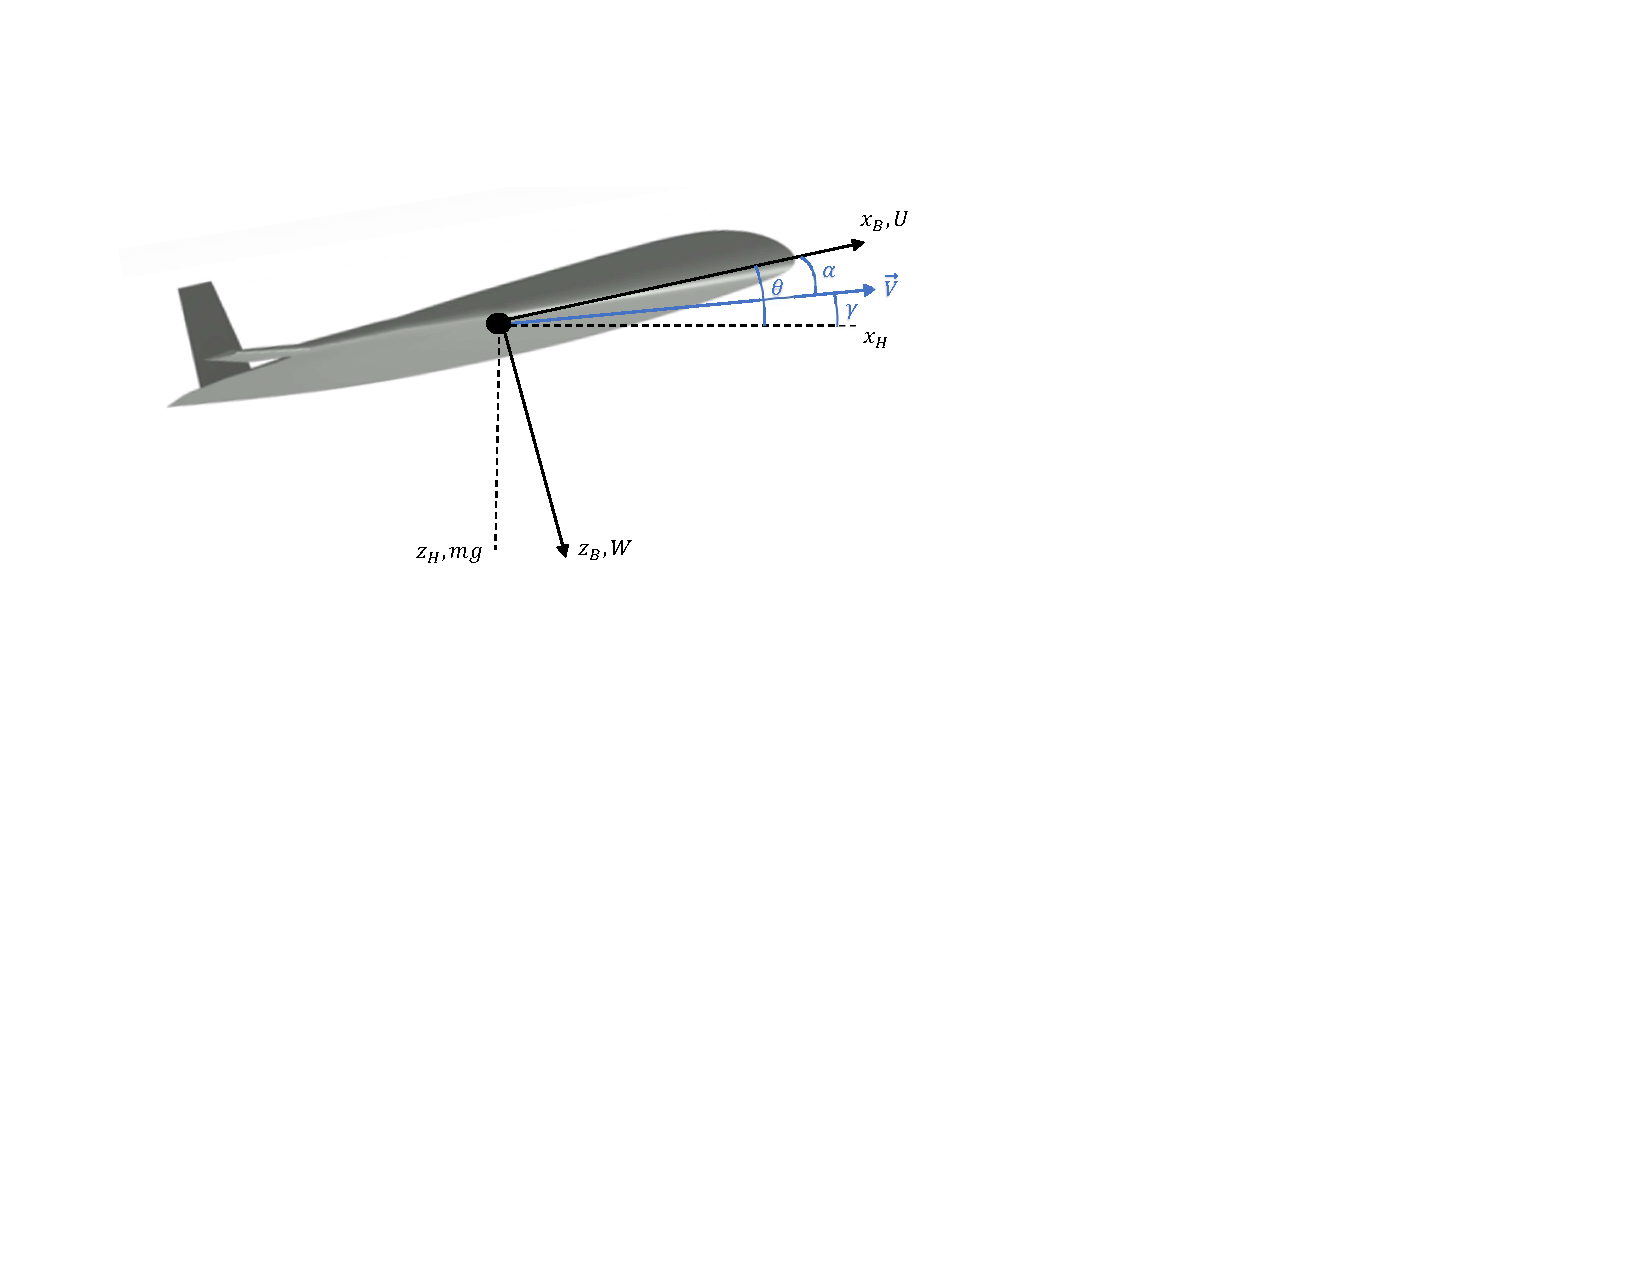
\includegraphics[scale=0.85]{Capitulo3/figs/angulo trayectoria_cropped.pdf}
\caption{ángulos de trayectoria de vuelo, cabeceo y ataque en plano simétrico x-z}
\label{fig: ángulos de vuelo, cabeceo y guiñada}
\end{figure}

el ángulo de la trayectoria de vuelo es la diferencia del ángulo de cabeceo menos el ángulo de ataque.  

\begin{equation}
\label{eq: trayectoria de vuelo}
    \gamma = \theta - \alpha    
\end{equation}

La transformación de $w$ en $\alpha$ para la dinámica longitudinal define el siguiente sistema dinámico longitudinal

\begin{align} 
\label{eq: modelo longitudinal alpha}
\dot V_T &= \frac{1}{mV}(X_u u + X_\alpha \alpha + X_q q + \textcolor{RoyalBlue}{X_{\delta_{e1}} \delta_{e1}}  + \textcolor{RoyalBlue}{X_{\delta_{e2}} \delta_{e2}}+ \textcolor{RoyalBlue}{X_{\delta_{T}} \delta_{T}}) - \frac{g}{V} S_{\theta} - q \alpha \\
\dot \alpha &= \frac{1}{mV}(Z_u u + Z_\alpha \alpha + Z_q q + \textcolor{RoyalBlue}{Z_{\delta_{e1}} \delta_{e1}}  + \textcolor{RoyalBlue}{Z_{\delta_{e2}} \delta_{e2}} + \textcolor{RoyalBlue}{Z_{\delta_{T}} \delta_{T}}) + \frac{g}{V} C_{\theta} + qu \\
\dot q &= \frac{1}{I_{y}}(M_u u + M_\alpha \alpha + M_q q + \textcolor{RoyalBlue}{M_{\delta_{elev_{i}}} \delta_{elev_{int}}}  + \textcolor{RoyalBlue}{M_{\delta_{T \Theta}} \delta_{T \Theta}})  \\
\dot \theta &= q
\end{align}

Para incluir la trayectoria de vuelo en la dinámica longitudinal se hace uso de \ref{eq: trayectoria de vuelo} en \ref{eq: modelo longitudinal alpha} último modelado longitudinal no-lineal

\begin{align} 
\label{eq: modelo longitudinal gamma}
\dot V_T &= \frac{1}{mV}(X_u u + X_\alpha \alpha + X_q q + \textcolor{RoyalBlue}{X_{\delta_{elev_{i}}} \delta_{elev_{i}}}  + \textcolor{RoyalBlue}{X_{\delta_{T \Theta}} \delta_{T \Theta}}) - \frac{g}{V} S_{\theta} - q \alpha \\
\dot \gamma &= -\frac{1}{mV}(Z_u u + Z_\alpha \alpha + Z_q q + \textcolor{RoyalBlue}{Z_{\delta_{elev_{i}}} \delta_{elev_{i}}} + \textcolor{RoyalBlue}{Z_{\delta_{T \Theta}} \delta_{T \Theta}}) - \frac{g}{V} C_{\theta} \\
\dot q &= \frac{1}{I_{y}}(M_u u + M_\alpha \alpha + M_q q + \textcolor{RoyalBlue}{M_{\delta_{elev_{i}}} \delta_{elev_{int}}}  + \textcolor{RoyalBlue}{M_{\delta_{T \Theta}} \delta_{T \Theta}}) \\
\dot \alpha &= q - \dot \gamma 
\end{align}


Cualquiera de los tres modelos dinámicos longitudinales no-lineales puede usarse dependiendo de las variables que buscamos obtener o la aplicación de control particular que queremos emplear. 

\bigskip
%%%%%%%%%%%%%%%%%%%%%%%%%%%%%%%%%%%%%%%%%%%%%%
\textbf{Modelo Dinámico No Lineal Lateral-Direccional - 3 GDL}\\
Ahora simplificaremos las ecuaciones del modelo de seis grados de libertad desacoplando la dinámica lateral-direccional, que considera tres grados de libertad: la traslación en el eje $y$ (desplazamiento lateral), la rotación en el eje $x$ (alabeo) y la rotación en el eje $z$ (guiñada). 
Para modelar y controlar la dinámica lateral-direccional no-lineal se consideran 4 variables del conjunto de ecuaciones: $v, p, r, \phi$. 


\begin{align} 
Y &= m (\dot v + ru - pw) \\
L &= \dot p I_x + \dot r I_{xz} + qr(I_z - I_y) - pq I_{xz} \\
N &=  \dot r I_z + \dot p I_{xz} + pq(I_y - I_x) + qr I_{xz}  \\
\dot \phi &= p + (q S_{\phi} + r C_{\phi}) tan_{\theta}
\end{align}

Se observa la dinámica lateral-direccional de 3 grados de libertad: 
\begin{itemize}
    \item desplazamiento lateral $v$
    \item momento angular de alabeo $p$
    \item momento angular de guiñada $r$
\end{itemize}

La variable de la actitud de alabeo $\phi$ es de referencia para concocer el nivel del ala de la aeronave, a través de la transformación del eje $y$ del cuerpo de la aeronave respecto el eje $y$ del plano horizonte local. El proceso de simplificación para la dinámica lateral-direccional no-lineal es un tanto más complejo que el longitudinal, dado que no podemos hacer cero los valores de actitud al cabeceo $\theta_{e}$, de altitud $w_{e}$ y de velocidad $u_{e}=V_{T}$, en su lugar debemos considerar estos valores constantes respecto a la condición de vuelo en equilibrio, de ahí el sufijo $e$.
Las ecuaciones de dinámica angular se simplifican de acuerdo con $q=0$ y \cite{Mohammad2020} considerando el producto de inercia $I_{xz}=0$. 

\begin{align} 
Y &= m (\dot v - u_{e}*r + w_{e}*p)\\
L &= \dot p I_x \\
N &=  \dot r I_z \\
\dot \phi &= p + r C_{\phi} tan_{\theta_{e}}
\end{align}

De la misma manera, seremos negligentes con las fuerzas lineales y angulares externas aplicadas en la dinámica longitudinal, obteniendo los términos de las fuerzas que tienen injerencia en la dinámica lateral-direccional. 

\begin{align}
    Y &= Y_{v} v + Y_{p}p + Y_{r} r + \textcolor{RoyalBlue}{Y_{\delta_{T} \delta_{T}}} + \textcolor{RoyalBlue}{Y_{\delta_{a1} \delta_{a1}}} + \textcolor{RoyalBlue}{Y_{\delta_{a2} \delta_{a2}}}  + \textcolor{RoyalBlue}{Y_{\delta_{r}r}} + Y_{G} G \\
    L &= L_{p}p + L_{r}r + L_{v}v + \textcolor{RoyalBlue}{L_{\delta_{a1} \delta_{a1}}} + \textcolor{RoyalBlue}{L_{\delta_{a2} \delta_{a2}}}  + \textcolor{RoyalBlue}{L_{\delta_{r}r}} \\
    N &= N_{p}p + N_{r}r + N_{v}v + \textcolor{RoyalBlue}{N_{\delta_{a1} \delta_{a1}}} + \textcolor{RoyalBlue}{N_{\delta_{a2} \delta_{a2}}}  + \textcolor{RoyalBlue}{N_{\delta_{r}r}}
\end{align}


Ahora vamos despejar respecto a las derivadas de las variables de estado. 

En la ecuación general obtenemos

\begin{align}
    \dot v & = \frac{1}{m}Y - u_{e} r + w_{e} p \\
    \dot p & = \frac{1}{I_x}L \\
    \dot r & = \frac{1}{I_z}N \\
    \dot \phi &= p + r C_{\phi} tan_{\theta_{e}}
\end{align}

Desarrollando las fuerzas laterales-direccionales en la dinámica no-lineal obtenemos las siguientes ecuaciones. 

\begin{align}
    \dot v & = \frac{1}{m}(Y_{v} v + Y_{\dot v}\dot v + Y_{p}p + Y_{r} r + \textcolor{RoyalBlue}{Y_{\delta_{T} \delta_{T}}} + \textcolor{RoyalBlue}{Y_{\delta_{a1} \delta_{a1}}} + \textcolor{RoyalBlue}{Y_{\delta_{a2} \delta_{a2}}}  + \textcolor{RoyalBlue}{Y_{\delta_{r}r}}) + gC_{\theta}S_{\phi} - u_{e}r + w_{e}p  \\
    \dot p & = \frac{1}{I_x}(L_{p}p + L_{r}r + L_{v}v + L_{\dot v}\dot v + \textcolor{RoyalBlue}{L_{\delta_{a1} \delta_{a1}}} + \textcolor{RoyalBlue}{L_{\delta_{a2} \delta_{a2}}}  + \textcolor{RoyalBlue}{L_{\delta_{r}r}}) \\
    \dot r & = \frac{1}{I_z}(N_{p}p + N_{r}r + N_{v}v + N_{\dot v}\dot v + \textcolor{RoyalBlue}{N_{\delta_{a1} \delta_{a1}}} + \textcolor{RoyalBlue}{N_{\delta_{a2} \delta_{a2}}}  + \textcolor{RoyalBlue}{N_{\delta_{r}r}})\\
    \dot \phi &= p + r C_{\phi} tan_{\theta_{e}}
\end{align}

Las ecuaciones anteriores describen la dinámica lateral-direccional no-lineal en el plano cuerpo de la aeronave. Para considerar dentro de este modelo el vector de velocidad definido en el plano de viento, tomamos la consideración  \ref{eq: ángulos aerodinámicos con pequeñas perturbaciones} y despejamos la variable de interés $\beta$ obteniendo el siguiente modelo. 

\begin{align}
    \dot \beta & = \frac{1}{mV}(Y_{\beta} \beta + Y_{p}p + Y_{r} r +   \textcolor{RoyalBlue}{Y_{\delta_{T} \delta_{T}}} + \textcolor{RoyalBlue}{Y_{\delta_{a1} \delta_{a1}}} + \textcolor{RoyalBlue}{Y_{\delta_{a2} \delta_{a2}}}  + \textcolor{RoyalBlue}{Y_{\delta_{r}r}}) + \frac{g}{V}C_{\theta}S_{\phi} - u_{e}r + w_{e}p  \\
    \dot p & = \frac{1}{I_x}(L_{p}p + L_{r}r + L_{\beta}\beta + L_{\dot \beta}\dot \beta + \textcolor{RoyalBlue}{L_{\delta_{a1} \delta_{a1}}} + \textcolor{RoyalBlue}{L_{\delta_{a2} \delta_{a2}}}  + \textcolor{RoyalBlue}{L_{\delta_{r}r}}) \\
    \dot r & = \frac{1}{I_z}(N_{p}p + N_{r}r + N_{\beta}\beta + N_{\dot \beta}\dot \beta + \textcolor{RoyalBlue}{N_{\delta_{a1} \delta_{a1}}} + \textcolor{RoyalBlue}{N_{\delta_{a2} \delta_{a2}}}  + \textcolor{RoyalBlue}{N_{\delta_{r}r}})\\
    \dot \phi &= p + r C_{\phi} tan_{\theta_{e}}
\end{align}


\section{Discusiones}

La selección adecuada de sistemas de referencia es fundamental para describir con precisión el movimiento y la orientación de las aeronaves durante el vuelo. Los sistemas de referencia elegidos proporcionan un marco de trabajo esencial para el análisis de cinemática y dinámica, y tienen un impacto significativo en la formulación de ecuaciones de movimiento.

El análisis cinemático permite la descripción matemática de la posición, velocidad y aceleración de la EHEKATL BWB en función del tiempo. Esta sección proporciona la base para comprender y predecir el comportamiento de la aeronave en vuelo, considerando variables como la orientación, traslación y rotación.

La formulación de las ecuaciones de dinámica es esencial para comprender cómo las fuerzas y momentos externos afectan el movimiento de la aeronave. El análisis de las fuerzas y momentos involucrados proporciona información crucial para la estabilidad, control y rendimiento de EHEKATL BWB.

El estudio de las fuerzas y momentos aplicados considera las interacciones con el entorno durante el vuelo, considerando las fuerzas aerodinámicas, de gravedad, de propulsión y de control; y como la aeronave responde a la aplicación de estas fuerzas. La comprensión detallada de estos aspectos es esencial para el diseño de sistemas de control efectivos y la seguridad en vuelo.

El modelo dinámico de la aeronave EHEKATL BWB en términos de definición de los parámetros de estabilidad y control, variables de estado y de control, y ecuaciones de movimiento; es la culminación de este capítulo. El modelo dinámico proporciona una herramienta base para la simulación y predicción del comportamiento de la aeronave en una amplia gama de condiciones de vuelo.

El análisis y modelado dinámico presentados en este capítulo forman la base para la implementación de sistemas de control y la evaluación del rendimiento de la aeronave EHEKATL BWB.

En la sección de apéndices \ref{linealizacion a} se desarrolla el proceso de linealización de acuerdo con las ecuaciones de movimiento de seis grados de libertad, y se desacoplan de igual manera el modelo lineal longitudinal y el modelo lineal lateral-direccional.





%%%%%%%%%%%%%%%%%%%%%%%%%%%%%%%%%%%%%%%%%%%%%%%%%%%%%%%%%%%%%%%%%%%%%%%%%
%                        Sistemas de Control de Vuelo (FCS)     %
%%%%%%%%%%%%%%%%%%%%%%%%%%%%%%%%%%%%%%%%%%%%%%%%%%%%%%%%%%%%%%%%%%%%%%%%%
\chapter{Diseño de Controladores}

El diseño de controladores es una disciplina dentro de la ingeniería aeroespacial que se enfoca en el desarrollo de sistemas de control para estabilizar y controlar el movimiento de vehículos aéreos, vehículos espaciales y cohetes.
Un controlador de vuelo es un sistema electrónico que utiliza sensores de aceleración, velocidad y posición para determinar la trayectoria tanto de vehículos tripulados como no tripulados.  El controlador genera un comando de referencia (puede ser manual, emitida por un piloto; o automática, emitida por una computadora) y en respuesta a este comando de referencia (también conocido como señal de seguimiento o trayectoria deseada)  actúan las entradas de control del vehículo para lograr o alcanzar el estado deseado desde un estado previo o condición inicial. En el caso de EHEKATL BWB, se establecieron las entradas de control primarias (elevadores, alerones, timones y motores) para controlar su movimiento. El objetivo principal del controlador de vuelo es asegurar que la aeronave vuele de manera estable y predecible, respondiendo a los comandos del piloto o siguiendo una trayectoria específica de forma autónoma.

Los controladores de vuelo se estructuran en dos partes: el sistema de medición y el sistema de control. El sistema de medición utiliza sensores para medir las variables de la aeronave como la velocidad, la altitud, la actitud y la orientación. Estos datos se procesan en el sistema de control que utiliza algoritmos para calcular los comandos necesarios para mantener la aeronave en su trayectoria deseada. Estos comandos se envían a los actuadores que se encargan de mover los efectores de control, como los motores y las superficies de control aerodinámicas.

Existen dos tipos de controladores de vuelo: lineales y no lineales. Los controladores lineales son sistemas de control que utilizan ecuaciones lineales. Estos controladores son simples y fáciles de implementar, pero están restringidos a un rango de operación y pueden no ser capaces de manejar ciertas perturbaciones fuera de su punto de equilibrio. 

Por otro lado, los controladores no lineales tratan de compensar dinámicas altamente no lineales y su objetivo es compensar esta dinámica por medio de controladores robustos y libres de modelo, sobretodo en aeronaves las cuales están sujetas a diversos tipos de perturbaciones o estados que requieren un mayor grado de libertad y maniobrabilidad. 
La elección entre un controlador lineal o no lineal depende de la aplicación específica y de las características del vehículo.
En resumen, el diseño de controladores de vuelo es esencial para asegurar que una aeronave vuele garantizando ciertas condiciones de operación y estabilidad.  

En este capítulo, se desarrollan los controladores de vuelo no lineales Backstepping y Adaptive Backstepping para EHEKATL BWB. Los parámetros aerodinámicos se obtienen con XFLR5, dónde para las simulaciones de vuelo se utiliza un punto de operación específico o momento en el tiempo, siendo entonces simulaciones de sistemas invariantes en el tiempo.   
El diseño y simulación de los controladores de vuelo se realiza en el lenguaje de programación PYTHON.


%%%%%%%%%%%%%%%%%%%%%%%%%
 \section{Backstepping}

Un método introducido y usado para explorar nuevas direcciones en el diseño de control de sistemas con dinámica no lineal es Backstepping. 
%
Los controladores Backstepping sintetizan un sistema dinámico no lineal complejo (aeronave) en subsistemas que están interconectados.
Por tanto,  el sistema dinámico de la aeronave se divide en una serie de subsistemas.
%
El objetivo de control con Backstepping es alcanzar mediante cascadas el control en conjunto de estos subsistemas, empezando por el último subsistema.
La salida del controlador se convierte en la entrada del siguiente subsistema, y el proceso continua hasta alcanzar el primer subsistema. 
%
Cada subsistema del controlador es diseñado para estabilizar y seguir la trayectoria deseada de ese subsistema. 
%
El controlador Backstepping es diseñado para estabilizar y controlar la dinámica de la aeronave. Podemos construir controladores de forma sistemática que manejen la dinámica compleja y las no linealidades del movimiento de la aeronave, además de garantizar la estabilidad, \cite{vanGils2015}. 

Los controladores de Backstepping para EHEKATL BWB son:
\begin{itemize}
    \item Controlador Backstepping longitudinal 3-GDL 
    \item Controlador Bacsktepping lateral-direccional 3-GDL
\end{itemize}

Con Backstepping podemos tener un único controlador lateral-direccional que considera las no linealidades y el acoplamiento lateral-direccional de acuerdo con la señal de respuesta de los alerones y timones. 

\medskip

%%%%%%%%%%%%%%%%%%%%%%%%%%%%%%%%%%%%%%%%%%%%
\textbf{Controlador Backstepping}\\
Para los Controladores Backstepping de EHEKATL BWB se utiliza la siguiente estructura para la representación del modelo dinámico no lineal en espacio de estados.

\begin{align}
\label{estructura backstepping 1}
    \dot x_{1} &= f_{1} + g_1 x_2 + h_1 u \\ \nonumber
    \dot x_{2} &= f_{2} + g_2 u
\end{align}

La ecuación \ref{estructura backstepping 1} permite representar las no linealidades del movimiento acoplado (entre velocidades lineales y angulares) en el producto de $g_1 x_2$, mientras permite mostrar la participación de las entradas de control en ambos subsistemas. 

Se definen los errores de estimación $z_1, z_2$ como la diferencia entre las variables de estado ($x_1, x_2$) y las señales de seguimiento deseadas ($x_1^d, x_2^d$). El error $z_3$ considera la dinámica de los actuadores, y se define como la diferencia entre la entrada de control real $u$ y el comando de referencia $u^d$.

\begin{align}
    z_1 &= x_1 - x^d_1 \\
    z_2 &= x_2 - x^d_2 \\
    z_3 &= u - u^d
\end{align}

Se define la función de transferencia de la dinámica de los actuadores considerando un retraso de primer orden: 

\begin{equation}
    \dot u = - \frac{1}{\tau}u + \frac{1}{\tau} u_c
\end{equation}

dónde: $\tau$=tiempo constante, $u_{c}$= comando de control generado por el controlador y $u$= comando real de la dinámica de los actuadores. 

Se propone una función candidata de Lyapunov para cada uno de los errores de estimación definidos en el paso anterior.

\begin{gather}
\label{Lyapunovn 1}
    V (z_1, z_2, z_3) =\frac{1}{2} z^T_1 z_1 + \frac{1}{2} z^T_2 z_2 + \frac{1}{2} z^T_3 z_3
\end{gather}

 Se procede a derivar la función candidata de Lyapunov propuesta en \ref{Lyapunovn 1}.

\begin{align}
       \dot V &= z^T_1 \dot z_1 + z^T_2 \dot z_2 + z^T_3 \dot z_3 \nonumber \\
        &= z^T_1 (\dot x_1 - \dot x^d_1) + z^T_2 (\dot x_2 - \dot x^d_2) + z^T_3 (\dot u - \dot u^d) \nonumber \\ 
    &= z^T_1 (f_1 + g_{1} x_2 + h_1 u - \dot x^d_1) + z^T_2 (f_2 + g_{2} u - \dot x^d_2) + z^T_3 (\frac{1}{\tau}(u_c - u) - \dot u^d) \nonumber \\
    &= z^T_1 (f_1 + g_{1} (z_2 + x_{2}^d) + h_1 (z_3 + u^d) - \dot x^d_1) + z^T_2 (f_2 + g_{2} (z_3 + u^d) - \dot x^d_2)\nonumber \\
    &+ z^T_3 (\frac{1}{\tau}(u_c - u) - \dot u^d)
\end{align}

Recordando el error $z_2 = x_2 - x^d_2$ se obtiene fácilmente $x_2 = z_2 + x^d_2$ para el primer subsistema, mientras que para el segundo subsistema tenemos que $z_3 = u - u^d$,  y por tanto $u = z_3 + u^d$. 

Una vez desarrollada la derivada de la función candidata de Lyapunov, se proponen las leyes de control virtual con el propósito de compensar los términos resultantes y agregar el término de control $k_n z_n$.
El término de control se compone por una matriz de ganancias $k_n$ conocida y definida como constante positiva,que multiplica al cuadrado del error de estimación $z_n$. El objetivo del término de control es obtener un amortiguamiento o disipación hasta alcanzar el valor deseado de la señal de seguimiento o comando de referencia. 

\begin{align}
\label{leyes de control 1}
    x^d_2 &= \frac{1}{g_{1}} [- f^T_1 + \dot x^d_1 - k_1 z_1] \nonumber \\
    u^d &= \frac{1}{g_{2}} [-f_{2}^T + \dot x_{2}^d - k_2 z_2 - g_{1}^T z_1] \nonumber \\
    u_c &= u + \tau [\dot u^d - g_{2}^T z_2 - (h_1^T u + h_{1}^T) z_1 - k_3 z_3]
\end{align}

Ahora se sustituyen las leyes de control virtual \ref{leyes de control 1} en la derivada de la función candidata de Lyapunov y se desarrolla.

\begin{align}
      \dot V &=  z^T_1 (f_1 + g_{1} (z_2 + [\frac{1}{g_{1}} [- f^T_1  + \dot x^d_1 - k_1 z_1]]) + h_1 z_3 + h_1 u - \dot x^d_1) \nonumber \\
      &+ z^T_2 (f_2 + g_{2} (z_3 + [\frac{1}{g_{2}} [-f_{2}^T + \dot x_{2}^d - k_2 z_2 - g_{1}^T z_1]]) - \dot x^d_2) \nonumber \\
      &+ z^T_3 (\frac{1}{\tau}([ u + \tau [\dot u^d - g_{2}^T z_2 - u h_1^T z_1 - h_{1}^T z_1 - k_3 z_3]] - u) - \dot u^d)
\end{align}

Entonces,

\begin{align}
    &= z^T_1 (g_1 z_2  + h_1 z_3 + h_1 u - k_1 z_1) + z^T_2 (g_2 z_3 - g^T_1 z_1 - k_2 z_2) \nonumber \\
      &+ z^T_3 (- u h_1^T z_1 - h_1^T z_1  - g_{2}^T - k_3 z_3) \nonumber \\
      &= (z^T_1g_1 z_2 - z^T_2 g^T_1 z_1 ) + (z_1^T(h_1 (z_3 + u)) - h_1^T(z_1(1+u))) \nonumber \\
      &- z^T_1 k_1 z_1 + (z^T_2 g_2 z_3 - z^T_3 g_{2}^T z_2 ) -  z^T_2 k_2 z_2 - z^T_3  k_3 z_3 \nonumber \\
      &= - z^T_1 k_1 z_1 - z^T_2 k_2 z_2 -  z^T_3  k_3 z_3
\label{backstepping eq}
\end{align}

se observa que las leyes de control virtual propuestas compensan correctamente los términos requeridos.
Después de aplicar las leyes de control virtual, la derivada de la función candidadata de Lyapunov se define: 

\begin{equation}
\label{Lyapunov sss}
    \dot V = - z^T_1 k_1 z_1 - z^T_2 k_2 z_2 -  z^T_3  k_3 z_3
\end{equation}

y por tanto: 

\begin{gather}
    \dot V \leqslant 0
\end{gather}

De acuerdo con el teorema de La Salle-Yoshizawa, los estados $z_1,z_2,z_3$ convergen asintóticamente al origen en medida que  $t\to\infty$. 
Esto es, $z_1=z_2 = z_3 \to 0$ lo que implica que $x_1\to x_1^d$, $x_2\to x_2^d$ y $u\to u^d$. En adición con la ecuación \ref{Lyapunov sss} tenemos que $z_1, z_2, z_3 \in L_2$. 

%Lyapunov introdujo la idea de una función de energía ficticia, denominada función de Lyapunov, aplicable a cualquier ecuación diferencial y tanto para sistemas lineales como no lineales. 
%En función del signo de la función de Lyapunov y de su derivada con respecto al tiempo, se pueden obtener conclusiones sobre el tipo de estabilidad de un estado de equilibrio. 
%Según Lyapunov, un sistema posee un estado de equilibrio en el origen si existe una función escalar $V(x)$ para el caso continuo o $V(x_k)$ para el caso discreto, con derivas parciales continuas y que satisfaga las siguientes condiciones

%\begin{itemize}
    %\item $V(x)$ o $V(x_k)$ es definida positiva
    %\item $\dot V(x)$ 0 $\dot V(x_{k+1})$ es definida semi-negativa
%\end{itemize}

%Entonces el estado de equilibrio en el origen es uniforme y asintóticamente estable. 

\medskip

Recordando las leyes de control virtual propuestas en \ref{leyes de control 1}, podemos observar que los subsistemas están relacionados con la derivada del subsistema anterior en las leyes de control virtual, entonces se visualiza esta cascada de dependencia entre el subsistema $n+1$ y el subsistema $n$.

Nuestro interés es calcular las derivadas de las variables de las señales de seguimiento o comandos de referencia $\dot x_1^d$ $\dot x_2^d$, y la derivada de la ley de control virtual propuesta para la dinámica de los actuadores $\dot u_d$.
El valor de $x_1^d$ es propuesto de acuerdo con la señal de seguimiento deseada.
Vamos a desarrollar el caso para cuando $x_1^d$ es un valor constante $c$.

\begin{align}
    x_1^d &= c \\ \nonumber
    \dot x_1^d &= 0 \nonumber
\end{align}

Para un valor constante de  $x_1^d$ dónde su derivada $\dot x_1^d$ se vuelve cero, podemos calcular $\dot x_2^d$. 

\begin{align}
    \dot x_2^d &= \frac{\partial x_2^d}{\partial f_1^T} \dot f^1 + \frac{ \partial x_2^d}{\partial \ddot x_1^d} \dot x_1^d + \frac{\partial x_2^d}{\partial z_1} \dot z_1 \nonumber \\
    &= \frac{d}{d f_1^T} (-\frac{1}{g_1} f_1^T) \dot f_1^T + \frac{d}{d \dot x_1^d} ( \frac{1}{g_1} \dot x_1^d) \ddot x_1^d + \frac{d}{d z_1} (-\frac{1}{g_1} k_1 z_1) \dot z_1 \nonumber \\
    &= -\frac{1}{g_1} \dot f_1^T + \frac{1}{g_1} \ddot x_1^d - \frac{1}{g_1} k_1 \dot z_1
\end{align}

Se asume que $\dot x_1 = \ddot x_1 = 0$ y $\dot f_1^T = 0$, por lo que únicamente se considera el término del error de estimación $z_1$.

\begin{gather}
\label{derivada control 1}
    \dot x_2^d = -\frac{1}{g_1} k_1 (g_1 z_2 + h_1 z_3 + h_1 u - k_1 z_1) 
\end{gather}

Calculando la derivada de $u^d$

\begin{align}
    \dot u^d &= - \frac{\partial u^d}{\partial{f_2^T}}  \dot f_2^T + \frac{\partial u^d}{\partial{\dot x_2^d}} \ddot x_2^d - \frac{\partial u^d}{\partial{z_2}} k_2 \dot z_2 - \frac{\partial u^d}{\partial{z_1}} g_1^T z_1 \nonumber \\
    &= - \frac{d}{df_2^T}(\frac{1}{g_2}f_2^T) \dot f_2^T + \frac{d}{\dot x_2^d} (\frac{1}{g_2}\dot x_2^d) \ddot x_2^d - \frac{d}{ z_2}(\frac{1}{g_2}k_2 z_2) \dot z_2 - \frac{d}{d z_1}  (\frac{1}{g_2} g_1^T z_1) \dot z_1 \nonumber \\
    &= -\frac{1}{g_2} \dot f_2^T + \frac{1}{g_2} \ddot x_2^d - \frac{1}{g_2} k_2 (g_2 z_3 - g_1^T z_1 - k_2 z_2) 
\end{align}

Y considerando que $\dot f_2^T=\ddot x_2^d=0$ 

\begin{equation}
\label{derivada control 2}
    \dot u_d = - \frac{1}{g_2} k_2 (g_2 z_3 - g_1^T z_1 - k_2 z_2)
\end{equation}

%Las conclusiones respecto a un análisis de estabilidad son las siguientes:
%$V$ es definida positiva, y $\dot V$ es definida semi negativa. $V$ es acotado dado que $z_1, z_2, z_3 \in L_\infty$. De acuerdo con el punto anterior y la dinámica del sistema $\dot x_1, \dot x_2 \in L_\infty$.
%Por tanto, $x_1, x_2$ son continuas uniformemente.
%
%De acuerdo con 
%$\dot V = - z_1^T k_1 z_1 - z_2^T k_2 z_2 - z_3^T k_3 z_3 \Rightarrow z_1, z_2, z_3 \in L_2$ 
%
%y por tanto 
%x_1, x_2, u, x_1^d, x_2^d, u^d, u_c \in L_2$. 
%
%En su forma integral
%$\int_0^t \dot V (z_1, z_2, z_3) dt = \int_0^t (- z_1^T k_1 z_1 - z_2^T k_2 z_2 - z_3^T k_3 z_3) dt = V(t) - V(0) \in L_\infty  \Rightarrow z_1, z_2, z_3 \in L_2$. 
%
%Esto implica que $V(t)\leq V(0)$, y por tanto, $z_1, z_2, z_3$ son acotadas.
%De acuerdo con el lema de Barbalat: Si la función diferenciable $f(t)$ tiene un límite finito cuanto $t \rightarrow \infty$, y si $\dot f(t)$ es uniformemente continua, entonces $\dot f(t) \rightarrow 0$ cuando $t \rightarrow \infty$.
%
%Recordando que una función es uniformemente continua si uno puede encontrar siempre una $\eta$ que no depende específicamente del punto $t_1$ y en particular, tal que $\eta$ no se reduzca cuando $t_1 \rightarrow \infty$.
%
%De lo anterior podemos concluir que como las variables de estado y los errores son acotados, por tanto, las salidas son acotadas y uniformemente continuas. 
%
%La validación de los teoremas de conversión normalmente asume que la solución del sistema es asequible, enunciaremos dos de ellos:
%
%Demostramos el teorema de estabilidad dado que el origen es estable demostrado a través de la función candidata de Lyapunov $V$ definida positiva y su derivada $\dot V$ definida como semi-negativa, así como también cumplimos el teorema de estabilidad exponencial, al tener constantes de ganancia estrictamente positivas.

\bigskip

\textbf{Controlador Backstepping Longitudinal}\\
De acuerdo con los desarrollos previos en el diseño del controlador Backstepping vamos a implementar la dinámica longitudinal de tres grados de libertad. 
Primeramente, se estructura la dinámica longitudinal en la representación mostrada en \ref{estructura backstepping 1}. 

\begin{equation}
    \begin{bmatrix}
        \dot u \\
        \dot \alpha
    \end{bmatrix}
    =
    \begin{bmatrix}
        \frac{1}{mV} (X_u u + X_\alpha \alpha + X_q q + T C_\theta) - \frac{g}{V} S_\theta \\
        \frac{1}{mV} (Z_u u + Z_\alpha \alpha + Z_q q + T S_\theta) + \frac{g}{V} C_\theta
    \end{bmatrix}
    +
    \begin{bmatrix}
    - \alpha & 0 \\
    u & 0
    \end{bmatrix}
    \begin{bmatrix}
      q  \\
      \theta
    \end{bmatrix}
    +
    \begin{bmatrix}
     \frac{1}{mV} X_{\delta_e1} & \frac{1}{mV} X_{\delta_e2} \\
     \frac{1}{mV} Z_{\delta_e1} & \frac{1}{mV} Z_{\delta_e2} \\
    \end{bmatrix}
    \begin{bmatrix}
        \delta_{e1} \\
        \delta_{e2} \\
    \end{bmatrix} \nonumber\\
\end{equation}

\begin{equation}
    \begin{bmatrix}
        \dot q \\
        \dot \theta
    \end{bmatrix}
    =
    \begin{bmatrix}
        \frac{1}{y} (M_u u + M_\alpha \alpha + M_q q) \\
        q \\
    \end{bmatrix}
    +
    \begin{bmatrix}
     \frac{1}{I_y} M_{\delta_{e1}} & \frac{1}{I_y} M_{\delta_{e2}} \\
      0 & 0 \\
    \end{bmatrix}
    \begin{bmatrix}
        \delta_{e1} \\
        \delta_{e2} \\
    \end{bmatrix}
\end{equation}

A través de simulaciones en XFLR5 se obtuvieron los coeficientes a-dimensionales de EHEKATL BWB mostrados en la Tabla \ref{Coeficientes a-dimensionales longitudinales de EHEKATL BWB}. 
\begin{table}[!h]
    \centering
    \begin{tabular}{|cc|cc|cc|}
    \hline
     $C_L$ & 0.33 & $C_D$ & 0.018 & $C_m$ & -0.001 \\
     \hline
     $C_{D_u}$ & -0.0067419 & $C_{D_\alpha}$ & 0.16364 & $C_{D_q}$ & 0.0 \\
     \hline
     $C_{L_u}$ & -0.0016445 & $C_{L_\alpha}$ & 2.5615 & $C_{L_q}$ & 2.6933 \\
     \hline
     $C_{M_u}$ & -2.8316e-08 & $C_{M_\alpha}$ & -0.33495 & $C_{M_q}$ & -0.9471 \\
     \hline
     $C_{L_{\delta_{e1,2}}}$ & 0.00029119 & $C_{D_{\delta_{e1,2}}}$ & -0.5852 & $C_{M_{\delta_{e1,2}}}$ & -0.2152 \\
     \hline
    \end{tabular}
    \caption{Coeficientes a-dimensionales longitudinales de EHEKATL BWB}
    \label{Coeficientes a-dimensionales longitudinales de EHEKATL BWB}
\end{table}

De acuerdo con los fórmulas de los coeficientes dimensionales longitudinales mostrados en la Tabla \ref{tab:derivadas dimensionales longitudinales}, se obtuvieron los coeficientes dimensionales para EHEKATL BWB calculados a partir de los coeficientes a-dimensionales previos en la Tabla \ref{Coeficientes a-dimensionales longitudinales de EHEKATL BWB}. 

\begin{table}[!h]
    \centering
    \begin{tabular}{|cc|cc|cc|}
    \hline
     $X_u$ & -0.000867816 & $X_\alpha$ & 0.0002289015 & $X_q$ & -0.0 \\
     \hline
     $Z_u$ & -0.01617908 & $Z_\alpha$ & -0.003549239 & $Z_q$ & -0.0001715658 \\
     \hline
     $M_u$ & -0.0016445 & $M_\alpha$ & -2.5615 & $M_q$ & -2.6933 \\
     \hline
     $X_{\delta_{e1}}$ & -4.0066025e-07 & $Z_{\delta_{e1}}$ & 0.0008052 & $M_{\delta_{e1}}$ & -0.00278488 \\
     \hline
     $X_{\delta_{e2}}$ & -4.0066025e-07 & $Z_{\delta_{e2}}$ & 0.0008052 & $M_{\delta_{e2}}$ & -0.00278488 \\
     \hline
    \end{tabular}
    \caption{Coeficientes dimensionales longitudinales de EHEKATL BWB}
    \label{Coeficientes dimensionales longitudinales de EHEKATL BWB}
\end{table}

De acuerdo con las leyes de control establecidas en \ref{leyes de control 1} y las derivadas en \ref{derivada control 1} y \ref{derivada control 2}, se realizaron las simulaciones mostradas en \ref{Simulación Backstepping Longitudinal de EHEKATL BWB} y \ref{Simulación Backstepping Altitud y Recorrido EHEKATL BWB}. 

Las ganancias sintonizadas para el controlador se muestran en \ref{ganancias backstepping longitudinal}.
Las ganancias $k_z$ son respecto a las variables de estado controlables $u, \alpha, q$ mientras $k_u$ para las entradas de control $\delta_{e1}, \delta_{e2}$. 
\begin{equation}
\label{ganancias backstepping longitudinal}
    k_u = 1.33, k_\alpha = 1.9, k_q = 1.33, k_{\delta_{e1}}=0.09,k_{\delta_{e2}}=0.09 
\end{equation}

El objetivo del controlador Bakstepping longitudinal de EHEKATL BWB en la simulación de la Figura \ref{Simulación Backstepping Longitudinal de EHEKATL BWB} es comandar según se desee el ángulo de ataque. 
Las condiciones iniciales utilizadas para la simulación de acuerdo con las variables de estado $u,\alpha, q,\theta$ y las entradas de control $\delta_{e1}, \delta_{e2}$ son todas cero. la variable $u$ representa los incrementos o decrementos de velocidad de acuerdo con la velocidad constante de $V=17.82 m/s$ y considerando un ángulo de ataque en equilibrio $\alpha_e$ de 1.88$^\circ$.

\begin{figure}[!h]
    \centering
    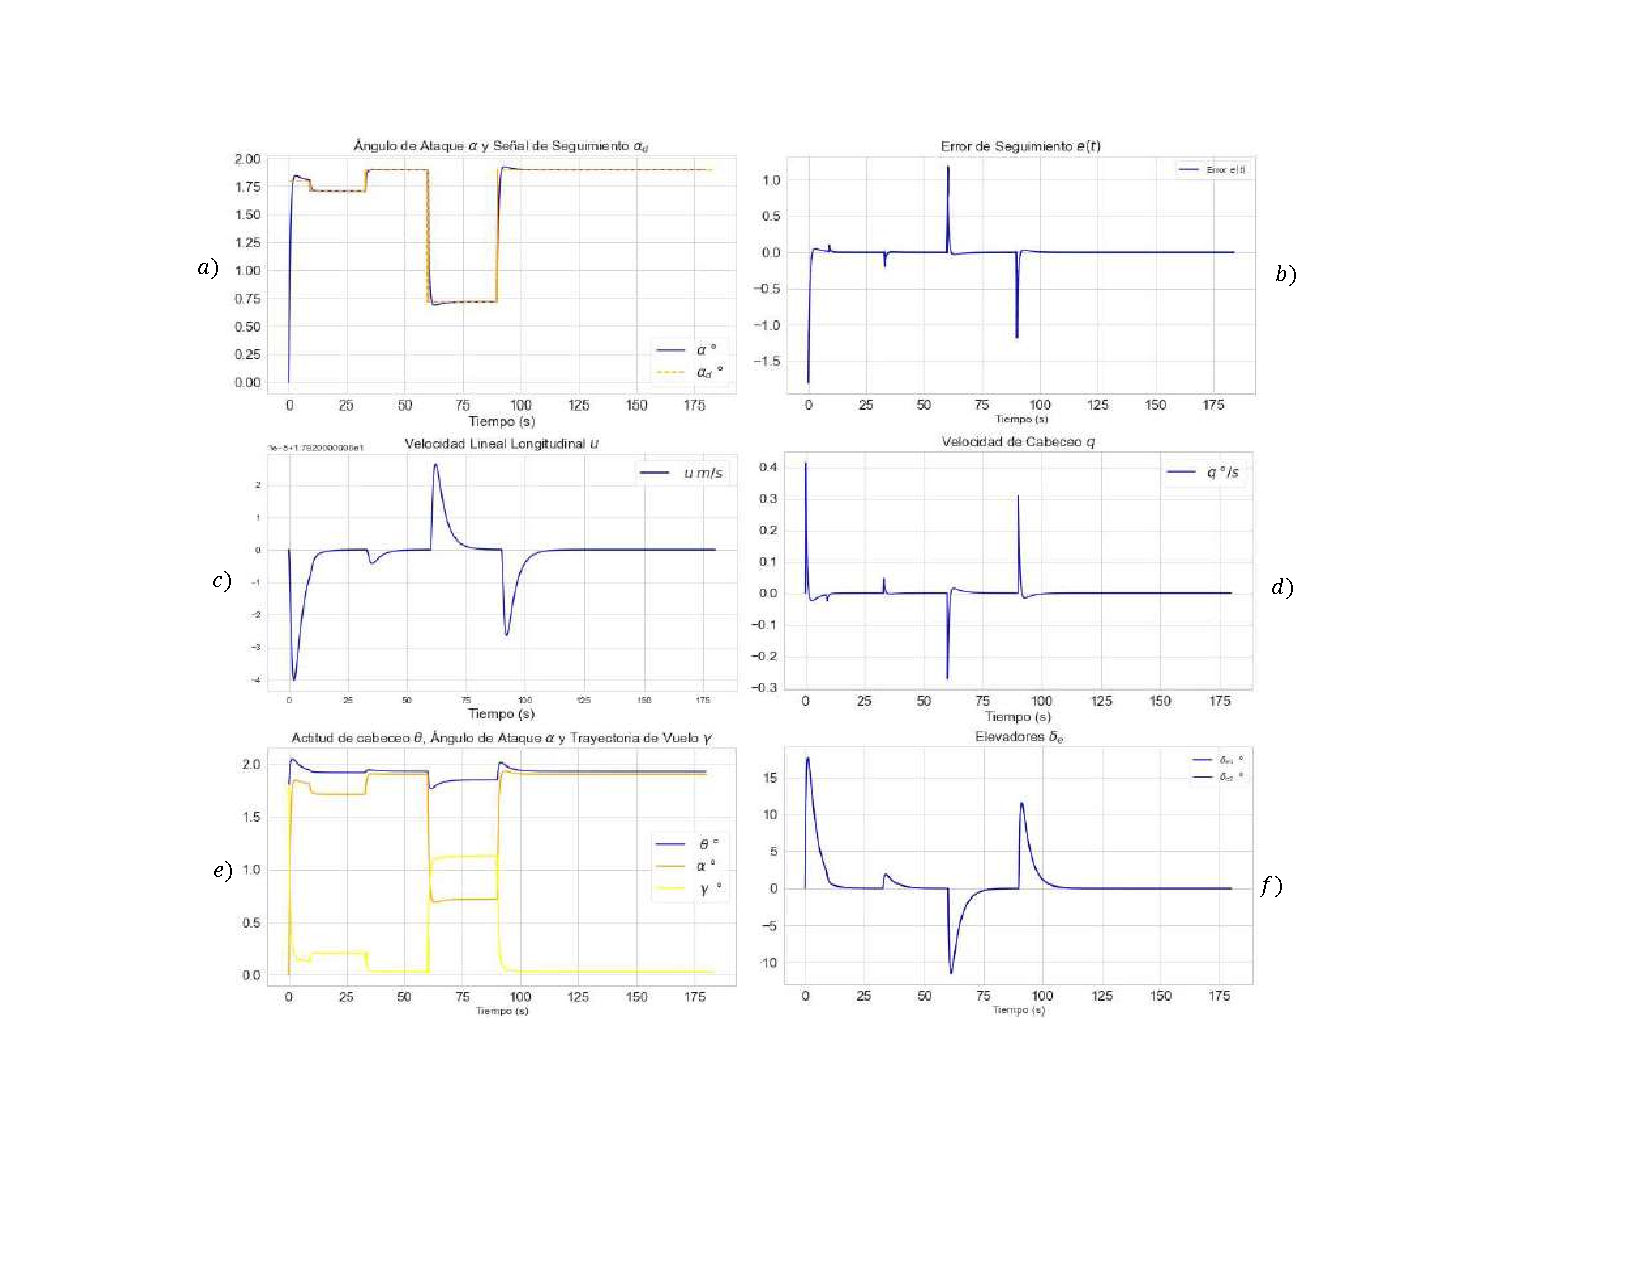
\includegraphics[scale=0.73]{Capitulo3/figs/Simulacion Backstepping Longitudinal 2_cropped.pdf}
    \caption{Simulación Backstepping Longitudinal de EHEKATL BWB}
    \label{Simulación Backstepping Longitudinal de EHEKATL BWB}
\end{figure}

\begin{figure}[!h]
\centering
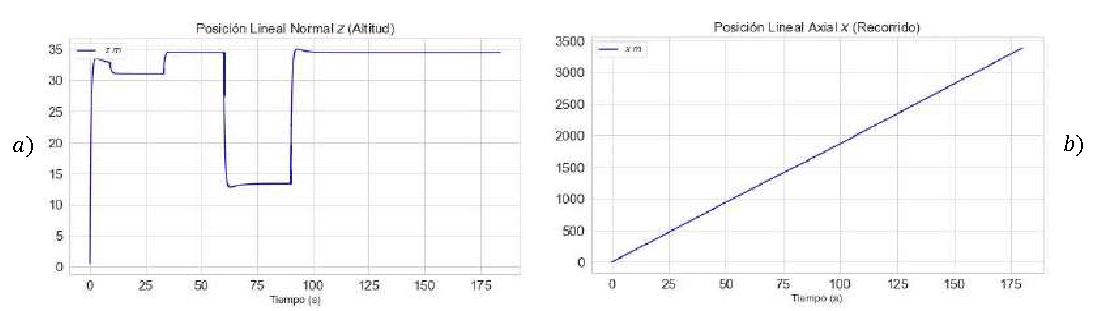
\includegraphics[scale=0.75]{Capitulo3/figs/Altitud y Recorrido Backstepping Longitudinal 2.pdf}
\caption{Simulación Backstepping Longitudinal - Altitud y Recorrido}
\label{Simulación Backstepping Altitud y Recorrido EHEKATL BWB}
\end{figure}

\textbf{Discusión de los Resultados:}
\begin{itemize}
    \item Al comenzar la simulación se observa en la gráfica a) que la trayectoria deseada para el ángulo de ataque $\alpha_d$ es un poco por debajo del ángulo de ataque en equilibrio $\alpha_e$, por lo que el ángulo de la trayectoria de vuelo $\gamma$ se eleva un poco respecto al horizonte local, sin embargo, después de los primeros veintisiete segundos $\gamma$ se aproxima a cero (o al horizonte) dado que $\alpha_d$ se aproxima a $\alpha_e$. Lo anterior describe un vuelo crucero, un vuelo recto y nivelado. Es importante recordar  que el ángulo de actitud de cabeceo y de trayectoria de vuelo son positivos en el sentido contrario de las manecillas respecto al plano de horizonte local. Sin embargo, el ángulo de ataque es positivo en sentido de la manecillas y a partir del plano cuerpo de EHEKATL BWB. Por tanto, los resultados tienen sentido y coherencia física.
    \item Cuando $\alpha$ desciende a $0.72$ el ángulo de la trayectoria de vuelo se direcciona un tanto hacia arriba, por el sentido físico que explicamos en los párrafos anteriores.
    \item En la gráfica c) el sentido físico de la velocidad lineal $u$ también tiene coherencia. Cuando la aeronave se direcciona hacia arriba $u$ desciende, y cuando la aeronave va nariz abajo la velocidad $u$ asciende. Esto gracias a que cada vez que el vector de velocidad de la aeronave se aproxime al vector de velocidad de gravedad, la aeronave ganará velocidad en $u$. En medida que suceda lo contrario, y a partir de nuestra referencia de vuelo (horizonte local en eje $x$), cada vez que el ángulo nariz arriba aumente la resistencia del aire será mayor y el ángulo entre la dirección del vector de velocidad de la aeronave respecto al vector de gravedad también aumenta, por lo que disminuye la velocidad de $u$. 
    Sin embargo, los parámetros aerodinámicos obtenidos en orden de la velocidad $u$ no representan una magnitud significativa en las simulaciones mostradas en \ref{Simulación Backstepping Longitudinal de EHEKATL BWB} dado que se valor es muy pequeño. 
    \item En la gráfica d) la velocidad angular de cabeceo $q$ también posee sentido físico al ser positiva cuando la actitud de cabeceo es positiva, y al ser negativa cuando al actitud de cabeceo disminuye. 
    \item En la gráfica f) la señal de respuesta de los elevadores  $\delta_{e1}$ $\delta_{e2}$ tienen prácticamente la misma deflexión, que oscila entre los $15$ y $-10$ grados de acuerdo con la señal de seguimiento del ángulo de ataque. 
    Los elevadores tienen un sentido positivo en dirección de las manecillas, es decir, cuando en respuesta la nariz de la aeronave va hacia arriba. Por deducción, cuando los elevador tienen un valor negativo el momento hace que la aeronave vaya nariz abajo.
    \item En \ref{Simulación Backstepping Altitud y Recorrido EHEKATL BWB} se observa la cinemática en el plano $x-z$. 
    De acuerdo con la variaciones en el ángulo de ataque, en la gráfica a) la aeronave oscila a una altitud entre $30-35m$ en los primeros 55 segundos, después desciende hasta los $14m$ aproximadamente, y vuelve ascender hasta los $35m$ para mantiene una altitud constante. 
    En la gráfica b) las variaciones de $u$ son tan pequeñas que son indescriptibles en la posición lineal $x$, por tanto, se observa con una pendiente totalmente lineal. 
\end{itemize}

\medskip

\textbf{Controlador Backstepping Lateral-Direccional}\\
Ahora se implementa el modelo dinámico lateral-direccional de tres grados de libertad en la estructura \ref{estructura backstepping 1} para su representación en espacio de estados.
\begin{equation}
    \begin{bmatrix}
        \dot \beta \\
        \dot \phi
    \end{bmatrix}
    =
    \begin{bmatrix}
        \frac{1}{mV} (Y_\beta \beta + Y_p p + Y_r r + T C_\theta) - \frac{g}{V} S_\theta \\
        p
    \end{bmatrix}
    +
    \begin{bmatrix}
    w_e & - u_e \\
    0 & 0
    \end{bmatrix}
    \begin{bmatrix}
      p  \\
      r
    \end{bmatrix}
    +
    \begin{bmatrix}
     \frac{1}{mV} Y_{\delta_a} & \frac{1}{mV} Y_{\delta_r} \\
      0 & 0 \\
    \end{bmatrix}
    \begin{bmatrix}
        \delta_{a} \\
        \delta_{r} \\
    \end{bmatrix} \nonumber\\
\end{equation}

\begin{equation}
    \begin{bmatrix}
        \dot p \\
        \dot r
    \end{bmatrix}
    =
    \begin{bmatrix}
        \frac{1}{x} (L_\beta \beta + L_p p + L_r r) \\
        \frac{1}{z} (N_\beta \beta + N_p p + N_r r) \\
    \end{bmatrix}
    +
    \begin{bmatrix}
      \frac{1}{x} L_{\delta_{a}} &  \frac{1}{x} L_{\delta_{r}} \\
      \frac{1}{z} N_{\delta_{a}} & \frac{1}{z} N_{\delta_{r}} \\
    \end{bmatrix}
    \begin{bmatrix}
        \delta_{a} \\
        \delta_{r} \\
    \end{bmatrix}
\end{equation}

Los coeficientes aerodinámicos laterales a-dimensionales para EHEKATL BWB se obtuvieron con XFLR5 y se muestran en la Tabla \ref{Coeficientes adimensionales laterales de EHEKATL BWB}. 
\begin{table}[!h]
    \centering
    \begin{tabular}{|cc|cc|cc|}
    \hline
     $C_{Y_\beta}$ & -0.30066 & $C_{Y_p}$ & -0.0422 & $C_{Y_r}$ & -0.193 \\
     \hline
     $C_{l_\beta}$ & -0.046761 & $C_{l_p}$ & -0.24566 & $C_{l_r}$ & 0.0343 \\
     \hline
     $C_{n_\beta}$ & 0.0848 & $C_{n_p}$ & -0.006445 & $C_{n_r}$ & -0.054 \\
     \hline
     $C_{Y_{\delta_a}}$ & 0.018585 & $C_{l_{\delta_a}}$ & 0.11009 & $C_{r_{\delta_a}}$ & 0.0032415 \\
     \hline
     $C_{Y_{\delta_r}}$ & 0.0228 & $C_{l_{\delta_r}}$ & 0.0406 & $C_{r_{\delta_r}}$ & -0.04523 \\
     \hline
    \end{tabular}
    \caption{Coeficientes a-dimensionales laterales-direccionales de EHEKATL BWB}
    \label{Coeficientes adimensionales laterales de EHEKATL BWB}
\end{table}

De acuerdo con los parámetros a-dimensionales obtenidos, utilizando las fórmulas para los parámetros dimensionales de \ref{tab:derivadas dimensionales laterales} se obtuvieron los resultados de la Tabla \ref{Coeficientes dimensionales laterales de EHEKATL BWB}.

\begin{table}[!h]
    \centering
    \begin{tabular}{|cc|cc|cc|}
    \hline
     ${Y_\beta}$ & -0.30066 & ${Y_p}$ & -0.0422 & ${Y_r}$ & -0.193 \\
     \hline
     ${L_\beta}$ & -0.046761 & ${L_p}$ & -0.24566 & ${L_r}$ & 0.0343 \\
     \hline
     ${N_\beta}$ & 0.0848 & ${N_p}$ & -0.006445 & ${N_r}$ & -0.054 \\
     \hline
     ${Y_{\delta_a}}$ & 0.018585 & ${L_{\delta_a}}$ & 0.11009 & ${N_{\delta_a}}$ & 0.0032415 \\
     \hline
     ${Y_{\delta_r}}$ & 0.0228 & ${L_{\delta_r}}$ & 0.0406 & ${N_{\delta_r}}$ & -0.04523 \\
     \hline
    \end{tabular}
    \caption{Coeficientes dimensionales laterales-direccionales de EHEKATL BWB}
    \label{Coeficientes dimensionales laterales de EHEKATL BWB}
\end{table}

La señal de referencia puede ser tanto para comandar el ángulo de derrape como el ángulo de alabeo. 
Las simulaciones de la Figura \ref{Simulación Backstepping Lateral-Direccional de EHEKATL BWB} muestran la respuesta de la dinámica lateral-direccional con un controlador Backstepping capaz de comandar señales de seguimiento de acuerdo a un ángulo de derrape y/o un ángulo de alabeo deseados. 

Las ganancias sintonizadas para el controlador Backstepping lateral-direccional se muestra en \ref{ganancias backstepping lateral-direccional}. 

\begin{equation}
\label{ganancias backstepping lateral-direccional}
    k_\beta = 0.9603, k_\phi = 0.0993, k_p = 0.03, k_r = 0.3, k_{\delta_a} = 0.9, k_{\delta_r} = 0.9
\end{equation}

\begin{figure}[!h]
    \centering
    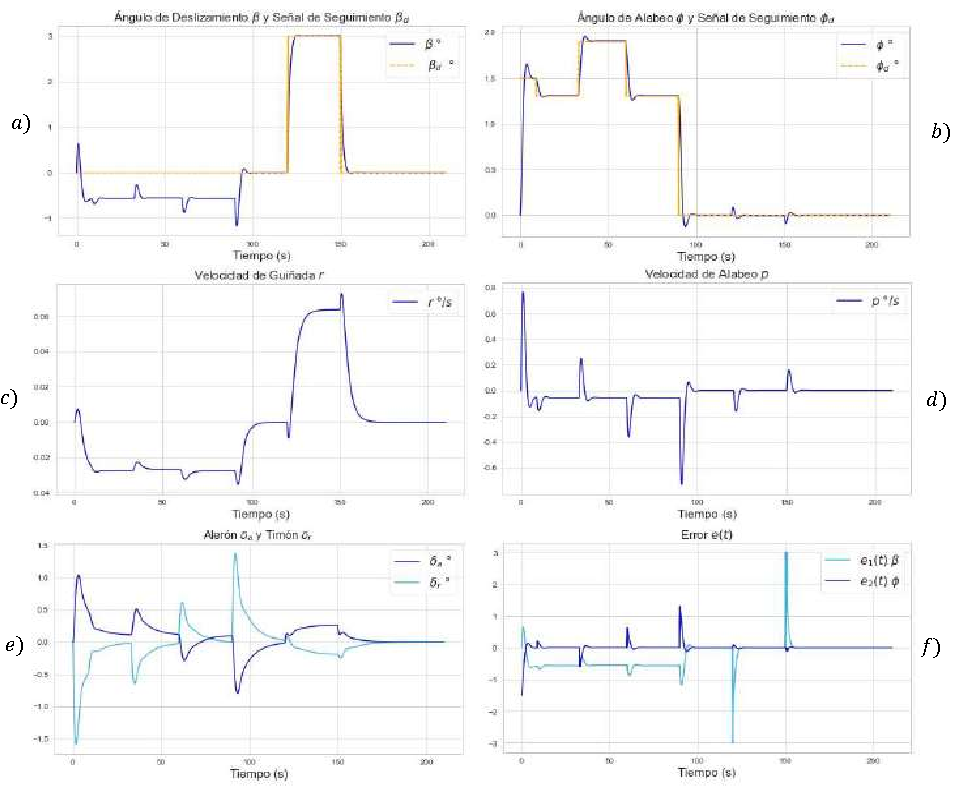
\includegraphics[scale=0.87]{Capitulo3/figs/Simulacion Backstepping LateralDireccional 2.pdf}
    \caption{Simulación Backstepping Lateral-Direccional de EHEKATL BWB}
    \label{Simulación Backstepping Lateral-Direccional de EHEKATL BWB}
\end{figure}

\begin{figure}[!h]
    \centering
    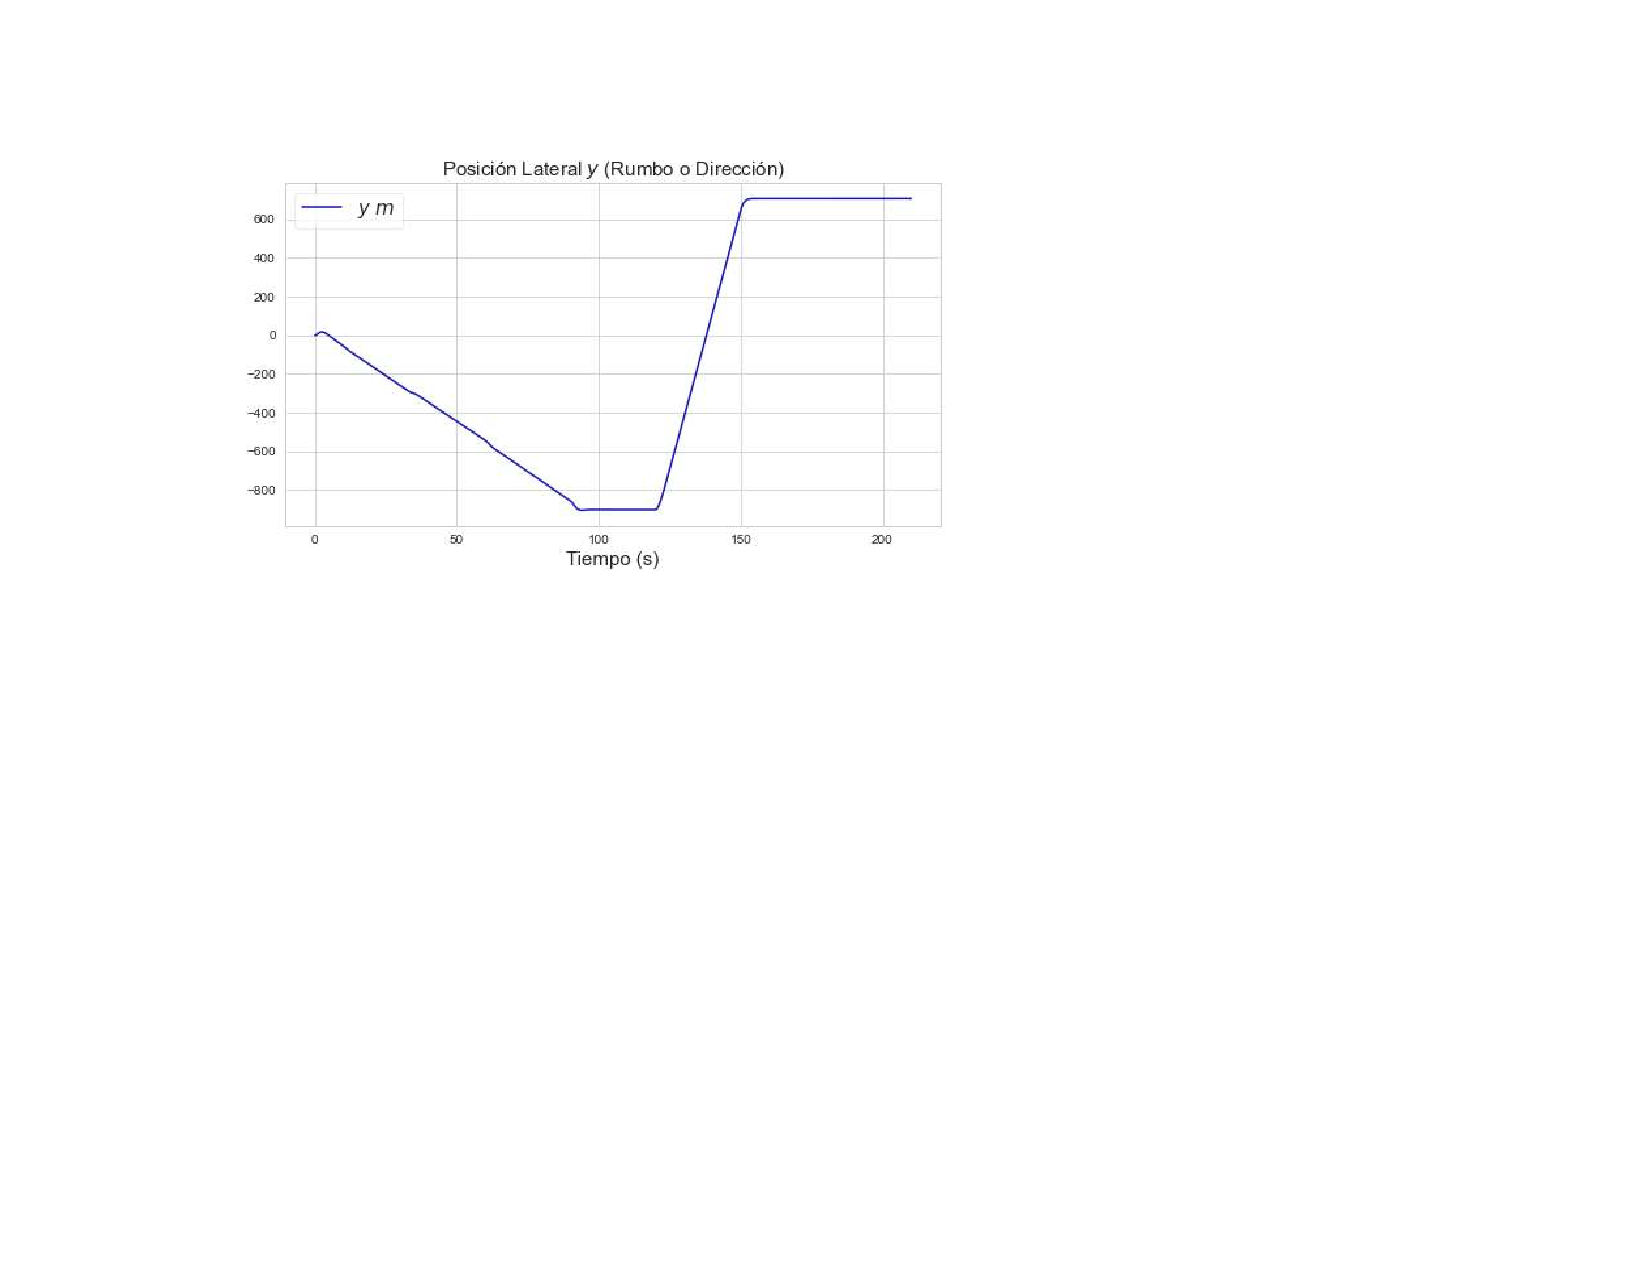
\includegraphics[scale=0.9]{Capitulo3/figs/Simulacion Backstepping LateralDireccional RumboDireccion_cropped.pdf}
    \caption{Simulación Backstepping Lateral-Direccional de EHEKATL BWB: Posición lateral $y$ (rumbo o dirección)}
    \label{Simulación Backstepping Lateral-Direccional de EHEKATL BWB: Posición lateral y (rumbo o dirección)}
\end{figure}

\textbf{Discusión de los Resultados:}
\begin{itemize}
    \item En la simulación \ref{Simulación Backstepping Lateral-Direccional de EHEKATL BWB} se demuestra en las gráficas a) y b) el seguimiento de ambos ángulos, $\beta$ y $\phi$, respectivamente; fundamentales en la dinámica lateral-direccional. 
    Primero, se comanda para EHEKATL BWB una señal de seguimiento para el ángulo de alabeo, dónde a través de una señal tipo paso se mantuvo en un alabeo de entre 1.3$^\circ$ - 1.9$^\circ$, en los primeros noventa segundos.
    \item Para el segundo ciento veinte, se comanda un ángulo de deslizamiento de 3$^\circ$ durante treinta segundos, para volver a un vuelo recto y nivelado con $\beta=0$ y $\phi=0$ y terminar la simulación.
    \item Se observa que la generación de un ángulo de alabeo $\phi$ tiene una respuesta en el ángulo de derrape $\beta$, quien define la orientación del vector de velocidad de EHEKATL BWB. De forma esperada, en la gráfica c) la velocidad de guiñada tiene una relación directa con el ángulo de derrape, mientras en la gráfica d) la velocidad de alabeo $p$ con el ángulo de alabeo propiamente. 
    \item En la gráfica e) la respuesta de los alerones es en el rango de 1$^\circ$ a -1$^\circ$, mientras la respuesta de los timones es de 1.5$^\circ$ a -1.5$^\circ$.
    \item En la gráfica f) el error de $\beta$ se mantiene fuera de seguimiento durante el seguimiento de la señal de alabeo, y con toda coherencia física, dado que el ángulo de alabeo genera esta respuesta en el ángulo de derrape, y por tanto este error es de esperarse. El comportamiento del error es muy rápido en aproximar la señal de seguimiento, y dada la complejidad de las no linealidades y el acoplamiento de la dinámica lateral-direccional se considera la sintonización de las ganancias del controlador Backstepping Lateral-Direccional como satisfactorias. 
    \item Finalmente, la Figura \ref{Simulación Backstepping Lateral-Direccional de EHEKATL BWB: Posición lateral y (rumbo o dirección)} muestra la posición lateral $y$, que en aeronáutica se conoce como rumbo o dirección, y dada la velocidad de $17.82 m/s$ proporciona tales resultados. El sentido negativo y positivo de $y$ coincide con el sentido de $\beta$. 
\end{itemize}


%%%%%%%%%%%%%%%%%%%%%%%%%%%%%%%%%%%%%%%%%%%%
\section{Backstepping Adaptable}

El término Adaptable, en cuanto a control se refiere, tiene la cualidad de ajustar parámetros y/o acciones de control con el objetivo de afrontar cambios, incertidumbres o variaciones en el sistema dinámico.
En la dinámica de las aeronaves, los coeficientes aerodinámicos son complejos de obtener con precisión, e incertidumbres y variaciones pueden presentarse a través del tiempo debido a factores como perturbaciones externas, cambios en los parámetros del sistema y condiciones ambientales. 

%Los principios básicos del diseño del controlador \textit{Adaptive Backstepping} de EHEKATL BWB envuelven tres componentes esenciales:
%\begin{itemize}
    %\item \textbf{Identificación del Sistema.} Vamos a considerar $f_1$ y $f_2$, funciones que describen las fuerzas y momentos aplicados en EHEKATL BWB como parámetros desconocidos.  
    %\item \textbf{Leyes de Adaptación.} De acuerdo con la identificación de $f_1$ $f_2$ las leyes de adaptación se diseñan para actualizar los parámetros del controlador. Las leyes de adaptación utilizan parámetros de estimación y el estado actual de las variables de estado del sistema para determinar cuanto ajustar las acciones de control de $\delta_e$ $\delta_a$ $\delta_r$
    %\item \textbf{Leyes de Control.} Las leyes de control son la pieza principal del controlador adaptable dado que generan las acciones de control de acuerdo con las variables de estado del sistema y los parámetros de adaptación. Combinan el proceso de adaptación con el objetivo de control (señal de seguimiento o comando de referencia), logrando la estabilidad del sistema y el desempeño deseado.
%\end{itemize}

La implementación de un controlador adaptable es adecuada para EHEKATL BWB dada la dinámica compleja del sistema dónde el conocimiento preciso de la dinámica del sistema puede ser un desafío, además de los cambios que experimentan estos mismos durante la operación de vuelo. 

\medskip

\textbf{Controlador Adaptive Backstepping}\\
Se representa la dinámica no lineal de EHEKATL BWB en la misma estructura utilizada para el controlador Bacsktepping. 

\begin{align}
    \dot x_{1} &= f_{1} + g_1 x_2 + h_1 u \\ \nonumber
    \dot x_{2} &= f_{2} + g_2 u \\ \nonumber
\end{align}

Se establecen los errores de estimación $\Tilde{f_1}$ $\Tilde{f_2}$ para estimar los valores $\hat{f_1}$ $\hat{f_2}$ de los parámetros desconocidos $f_1$ $f_2$. 
\begin{gather}
    \Tilde{f_1} =f_1 - \hat{f_1}\\ \nonumber
    \Tilde{f_2} = f_2 - \hat{f_2} \nonumber
\end{gather}

dónde

$\hat{f_1}$ y $\hat{f_2}$ son los valores estimados de $f_1$ y $f_2$.

$\Tilde{f_1}$ y $\Tilde{f_2}$ son los errores de estimación de $f_1$ y $f_2$.


Definimos tres bloques de errores de estimación: 1) $z_1, z_2$ para las variables de estado respecto a las señales de seguimiento, 2) $z_3$ para el comando de las entradas de control $u$ respecto a la ley de control virtual $u^d$ y 3) $\Tilde{f_1}, \Tilde{f_2}$ referente a las funciones con incertidumbre de fuerzas y momentos de EHEKATL BWB $f_1, f_2$ respecto a sus funciones de estimación $\hat{f_1}, \hat{f_2}$. 

\begin{align}
\label{errorres de estimacion adaptive}
    z_1 &= x_1 - x^d_1 \\ \nonumber
    z_2 &= x_2 - x^d_2 \\ \nonumber
    z_3 &= u - u^d \\ \nonumber
    \Tilde{f_1} &= f_1 - \hat{f_1} \\ \nonumber
    \Tilde{f_2} &= f_2 - \hat{f_2} \\ \nonumber
\end{align}

El error $z_3$ deriva de nuestra consideración de la dinámica de los actuadores, dónde consideramos un retraso de primer orden. La $u$ real considerada en la dinámica de los actuadores es producida por el siguiente proceso. Definiremos la función de transferencia de la dinámica de los actuadores: 

\begin{equation}
    \dot u = - \frac{1}{\tau}u + \frac{1}{\tau} u_c
\end{equation}

dónde:

$\tau:$ \textit{tiempo constante}


$u_{c}:$ \textit{comando de control generado por el controlador} 


$u:$ \textit{comando real de la dinámica de los actuadores}


Proponemos una función candidata de Lyapunov para cada uno de los errores de estimación definidos en \ref{errorres de estimacion adaptive}. 
\begin{equation}
    V_1 (z_1, z_2, z_3, \Tilde{f_1}, \Tilde{f_2}) = \frac{1}{2} z_1^T z_1 + \frac{1}{2} z_2^T z_2 + \frac{1}{2} z_3^T z_3 + \frac{1}{2} \Tilde{f_1^T} \Gamma_1 \Tilde{f_1} + \frac{1}{2} \Tilde{f_2^T} \Gamma_2 \Tilde{f_2}
\label{lyapunov 2}
\end{equation}

Para los errores de estimación $z_1, z_2,z_3$ vamos a proponer leyes de control virtual que compensen los términos de la ecuación y además contengan el término del controlador $k_n, z_n$. 
para los errores de estimación $ \Tilde{f_1}, \Tilde{f_2}$ vamos a proponer leyes de adaptación que compensen los términos a través de parámetros con ganancias de estimación. 

Primero, derivamos la función candidata de Lyapunov propuesta en \ref{lyapunov 2}. 
\begin{align}
       \dot V &= z^T_1 \dot z_1 + z^T_2 \dot z_2 + z^T_3 \dot z_3 + \Tilde{f_1^T}  \Gamma_1 \dot{\Tilde{f_1}} + \Tilde{f_2^T} \Gamma_2 \dot{\Tilde{f_2}} \nonumber \\
        &= z^T_1 (\dot x_1 - \dot x^d_1) + z^T_2 (\dot x_2 - \dot x^d_2) + z^T_3 (\dot u - \dot u^d) + \Tilde{f_1^T}  \Gamma_1 \dot{\Tilde{f_1}} + \Tilde{f_2^T} \Gamma_2 \dot{\Tilde{f_2}} \nonumber \\ 
    &= z^T_1 (f_1 + g_{1} x_2 - \dot x^d_1) + z^T_2 (f_2 + g_{2} u - \dot x^d_2) + z^T_3 (\frac{1}{\tau}(u_c - u) - \dot u^d) + \Tilde{f_1^T}  \Gamma_1 \dot{\Tilde{f_1}} + \Tilde{f_2^T} \Gamma_2 \dot{\Tilde{f_2}} \nonumber \\
    &= z^T_1 (f_1 + g_{1} (z_2 + x_{2}^d)  + h_1 z_3 + h_1 u - \dot x^d_1) + z^T_2 (f_2 + g_{2} (z_3 + u^d) - \dot x^d_2)  \nonumber \\
    &+ z^T_3 (\frac{1}{\tau}(u_c - u) - \dot u^d) + \Tilde{f_1^T}  \Gamma_1 \dot{\Tilde{f_1}} + \Tilde{f_2^T} \Gamma_2 \dot{\Tilde{f_2}}
\end{align}


De acuerdo con el desarrollo previo, proponemos las siguientes leyes de control de virtual. 

\begin{align}
    x^d_2 &= \frac{1}{g_{1}} [- \hat{f_1^T} + \dot x^d_1 - k_1 z_1] \nonumber \\
    u^d &= \frac{1}{g_{2}} [- \hat{f_2^T} + \dot x_{2}^d - k_2 z_2 - g_{1}^T z_1] \nonumber \\
    u_c &= u + \tau [\dot u^d - g_{2}^T z_2 - (h_1^Tu + h_1^T)z_1 - k_3 z_3]
\end{align}

substituimos y continuamos el desarrollo.  

\begin{align}
      \dot V &=  z^T_1 (f_1 + g_{1} (z_2 + [\frac{1}{g_{1}} [- \hat{f_1^T}  + \dot x^d_1 - k_1 z_1]]) + h_1 z_3 + h_1 u - \dot x^d_1) \nonumber \\
      &+ z^T_2 (f_2 + g_{2} (z_3 + [\frac{1}{g_{2}} [- \hat{f_2^T} + \dot x_{2}^d - k_2 z_2 - g_{1}^T z_1]]) - \dot x^d_2) \nonumber \\
      &+ z^T_3 (\frac{1}{\tau}([ u + \tau [\dot u^d - g_{2}^T z_2 - u h_1^T z_1 - h_{1}^T z_1 - k_3 z_3]] - u) - \dot u^d) \nonumber \\
      &+ \Tilde{f_1^T}  \Gamma_1 \dot{\Tilde{f_1}} + \Tilde{f_2^T} \Gamma_2 \dot{\Tilde{f_2}} \nonumber \\
      &= z^T_1 (\Tilde{f_1} + g_1 z_2  + h_1 z_3 + h_1 u - k_1 z_1) + z^T_2 (\Tilde{f_2} \nonumber \\
      &+ g_2 z_3 - g^T_1 z_1 - k_2 z_2) + z^T_3 (- u h_1^T z_1 - h_1^T z_1  - g_{2}^T - k_3 z_3) \nonumber \\
      &+ \Tilde{f_1^T}  \Gamma_1 \dot{\Tilde{f_1}} + \Tilde{f_2^T} \Gamma_2 \dot{\Tilde{f_2}} \nonumber \\
      &= z^T_1 \Tilde{f_1} + (z^T_1g_1 z_2 - z^T_2 g^T_1 z_1 ) + (z_1^T(h_1 (z_3 + u)) - h_1^T(z_1(1+u))) - z^T_1 k_1 z_1 + z^T_2 \Tilde{f_2} \nonumber \\ 
      &+ (z^T_2 g_2 z_3 - z^T_3 g_{2}^T z_2 ) -  z^T_2 k_2 z_2 - z^T_3  k_3 z_3 + \Tilde{f_1^T}  \Gamma_1 \dot{\Tilde{f_1}} + \Tilde{f_2^T} \Gamma_2 \dot{\Tilde{f_2}} \nonumber \\
      &= z^T_1 \Tilde{f_1} + z^T_2 \Tilde{f_2} - z^T_1 k_1 z_1 - z^T_2 k_2 z_2 -  z^T_3  k_3 z_3  + \Tilde{f_1^T}  \Gamma_1 \dot{\Tilde{f_1}} + \Tilde{f_2^T} \Gamma_2 \dot{\Tilde{f_2}}
\end{align}

Podemos apreciar los términos $\Tilde{f_1^T}  \Gamma_1 \dot{\Tilde{f_1}} ,  \Tilde{f_2^T} \Gamma_2 \dot{\Tilde{f_2}}$.
Vamos a compensarlos proponiendo las siguientes leyes de adaptación. 

\begin{gather}
    \dot{\Tilde{f_1}} = \dot f_1 - \dot{\hat{f_1}} = - \Gamma_{1}^{-1} z_1 \\ \nonumber
    \dot{\Tilde{f_2}} = \dot f_2 - \dot{\hat{f_2}} = - \Gamma_{2}^{-1} z_2 \nonumber
\end{gather}

Substituyendo las leyes de adaptación, terminamos el desarrollo de la derivada de la función candidata de Lyapunov.  

\begin{align}
      \dot V &= z^T_1 \Tilde{f_1} + z^T_2 \Tilde{f_2} - z^T_1 k_1 z_1 - z^T_2 k_2 z_2 -  z^T_3  k_3 z_3  + \Tilde{f_1^T}  \Gamma_1 (- \Gamma_{1}^{-1} z_1) + \Tilde{f_2^T} \Gamma_2 (- \Gamma_{2}^{-1} z_2) \nonumber \\ 
      &= z^T_1 \Tilde{f_1} + z^T_2 \Tilde{f_2} - z^T_1 k_1 z_1 - z^T_2 k_2 z_2 -  z^T_3  k_3 z_3  - \Tilde{f_1^T} z_1 - \Tilde{f_2^T} z_2 \nonumber \\
      &= - z^T_1 k_1 z_1 - z^T_2 k_2 z_2 -  z^T_3  k_3 z_3
\end{align}

\begin{equation}
\label{adapt lya yeah}
    \dot V = - z^T_1 k_1 z_1 - z^T_2 k_2 z_2 -  z^T_3  k_3 z_3 \\
\end{equation}

Y por tanto:
\begin{equation}
    \dot V \leqslant 0
\end{equation}

De acuerdo con el teorema de La Salle-Yoshizawa, los estados $z_1,z_2,z_3$ convergen asintóticamente al origen en medida que  $t\to\infty$. 
Esto es, $z_1=z_2 = z_3 \to 0$ lo que implica que $x_1\to x_1^d$, $x_2\to x_2^d$ y $u\to u^d$. En adición con la ecuación \ref{adapt lya yeah} tenemos que $z_1, z_2, z_3 \in L_2$. 

\medskip

\textbf{Controlador Adaptive Backstepping Longitudinal}\\
Para el diseño del controlador Adaptive Backstepping longitudinal de EHEKATL BWB se implementa la señal de seguimiento del régimen de ascenso, conocido por sus siglas en inglés como $ROC$.
En el controlador Backstepping Longitudinal comandamos la señal de ángulo de ataque considerando el modelo dinámico con ejes viento, ahora comandamos la velocidad linear normal $w$ sinónima a $ROC$ considerando el modelo dinámico en los ejes cuerpo. 
La diferencia entre una aplicación y otra es el uso de los sistemas de referencia.

La estructura en representación de estados de acuerdo con la dinámica no lineal longitudinal de EHEKATL BWB queda representada de la siguiente manera. 

\begin{equation}
    \begin{bmatrix}
        \dot u \\
        \dot w
    \end{bmatrix}
    =
    \begin{bmatrix}
        \frac{1}{m} (X_u u + X_w w + X_q q + T C_\theta) - \frac{g}{V} S_\theta \\
        \frac{1}{m} (Z_u u + Z_w w + Z_q q + T S_\theta) + \frac{g}{V} C_\theta
    \end{bmatrix}
    +
    \begin{bmatrix}
    - w & 0 \\
    u & 0
    \end{bmatrix}
    \begin{bmatrix}
      q  \\
      \theta
    \end{bmatrix}
    +
    \begin{bmatrix}
     \frac{1}{m} X_{\delta_e1} & \frac{1}{m} X_{\delta_e2} \\
     \frac{1}{m} Z_{\delta_e1} & \frac{1}{m} Z_{\delta_e2} \\
    \end{bmatrix}
    \begin{bmatrix}
        \delta_{e1} \\
        \delta_{e2} \\
    \end{bmatrix} \nonumber\\
\end{equation}

\begin{equation}
    \begin{bmatrix}
        \dot q \\
        \dot \theta
    \end{bmatrix}
    =
    \begin{bmatrix}
        \frac{1}{y} (M_u u + M_w w + M_q q) \\
        q \\
    \end{bmatrix}
    +
    \begin{bmatrix}
     \frac{1}{I_y} M_{\delta_{e1}} & \frac{1}{I_y} M_{\delta_{e2}} \\
      0 & 0 \\
    \end{bmatrix}
    \begin{bmatrix}
        \delta_{e1} \\
        \delta_{e2} \\
    \end{bmatrix}
\end{equation}

De acuerdo a las simulaciones aerodinámicas con XFLR5 obtuvimos los parámetros dimensionales de EHEKATL BWB. 

\begin{table}[!h]
    \centering
    \begin{tabular}{|cc|cc|cc|}
    \hline
     $X_u$ & -0.027843 & $X_w$ & 0.34641 & $X_q$ & 0.0 \\
     \hline
     $Z_u$ & -1.5092 & $Z_w$ & -17.434 & $Z_q$ & -5.415 \\
     \hline
     $M_u$ & 6.1021e-07 & $M_w$ & -2.5615 & $M_q$ & -1.1697 \\
     \hline
     $X_{\delta_{e1}}$ & 0.30605 & $Z_{\delta_{e1}}$ &-8.8438 & $M_{\delta_{e1}}$ & -2.3445 \\
     \hline
     $X_{\delta_{e2}}$ & 0.30605 & $Z_{\delta_{e2}}$ & -8.8438 & $M_{\delta_{e2}}$ & -2.3445 \\
     \hline
    \end{tabular}
    \caption{Coeficientes dimensionales longitudinales de EHEKATL BWB 2}
    \label{Coeficientes dimensionales longitudinales de EHEKATL BWB adaptive}
\end{table}

El objetivo de la simulación de la Figura \ref{Simulación para la dinámica longitudinal de EHEKATL BWB con el controlador Adaptive Backstepping} es comandar ROC para lograr ascender y descender a EHEKATL BWB. 

De acuerdo con los resultados de \ref{Coeficientes dimensionales longitudinales de EHEKATL BWB adaptive} se establece una velocidad constante de $V_T = 17 m/s$ con un ángulo de actitud en equilibrio de $\theta_e = 1.8$. 

Las ganancias de las leyes de control virtual y de las leyes de adaptación se muestran en \ref{ganancias adaptive backstepping longitudinal}.
\begin{align}
\label{ganancias adaptive backstepping longitudinal}
    k_u = 1.5, k_w = 1.5, k_q = 1.5, k_\theta = 0.3 \\ \nonumber
    k_{\delta_{e_u}} = 120, k_{\delta_{e_w}} = 120, k_{\delta_{e_q}} = 120, k_{\delta_{e_\theta}} = 60 \\ \nonumber
    \Gamma_u = 12, \Gamma_w = 15, \Gamma_q = 15, \Gamma_\theta = 9 \nonumber
\end{align}


\begin{figure}[!t]
    \centering
    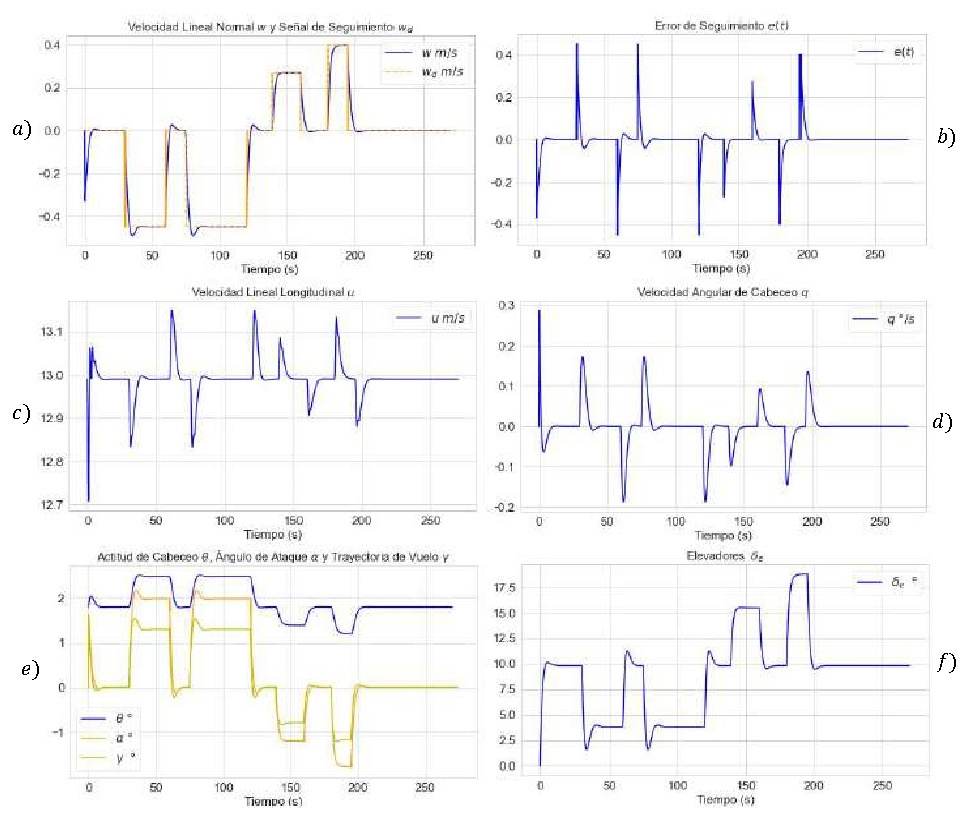
\includegraphics[scale=0.86]{Capitulo3/figs/Simulacion Adaptive Backstepping Longitudinal 2.pdf}
    \caption{Simulación para la dinámica longitudinal de EHEKATL BWB con el controlador Adaptive Backstepping}
    \label{Simulación para la dinámica longitudinal de EHEKATL BWB con el controlador Adaptive Backstepping}
\end{figure}

\textbf{Discusión de Resultados:}
\begin{itemize}
    \item En la gráfica a) la señal de seguimiento $w_d$ comanda el régimen de ascenso para EHEKATL BWB. Es importar recordar que el eje cuerpo $z$ se dirige hacia abajo, por lo que el ascenso se define con $-w$, mientras que el descenso se define con $+w$. 
    \item El tiempo de simulación es de 270 segundos. La señal de seguimiento $w_d$ es una señal tipo paso con dos ascensos y dos descensos, terminando en una altitud constante.
    \item La primer fila de las ganancias sintonizan a la ley de control de la dinámica de la aeronave, las ganancias de la segunda fila sintonizan la ley de control de la dinámica de los actuadores, para finalmente, las ganancias de la tercer fila sintonizar la ley de adaptación de los parámetros desconocidos.
    \item En la gráfica f) cuando la simulación comienza los elevadores tienen una deflexión de $-10$ grados, pero justo después se ajusta a $0$ grados dónde se mantiene el vuelo a altitud constante. 
    Cuando el régimen de ascenso comienza (valor de $w$ negativo) los elevadores hacen deflexión con valor negativo, mientras el ángulo de actitud y el ángulo de ataque son positivos, de acuerdo con su marco de referencia. 
    \item en la gráfica e) la trayectoria de vuelo se define como la diferencia entre la actitud de cabeceo y el ángulo de ataque, entonces, en el primer instante de la simulación se percibe el ajuste en los tres ángulos de acuerdo con la deflexión de los elevadores. Después se mantiene la actitud de cabeceo de equilibrio de $1.88$ para un vuelo a altitud constante. 
    \item Cuando se generan los primeros dos pasos del ángulo de ataque se observa que incrementa la actitud de cabeceo pero en una razón menor y la trayectoria de vuelo incrementa con un ángulo positivo, en relación al incremento de altitud que se está obteniendo. 
    \item Cuando se genera un ángulo de ataque negativo a velocidad constante, quiere decir que ahora el vector de velocidad está por encima de la aeronave, y el ángulo de la trayectoria de vuelo también es negativo resultado en una altitud descendiente. 
    \item Finalmente, en la Figura \ref{Trayectoria para la dinámica longitudinal de EHEKATL BWB con el controlador Adaptive Backstepping} se observa la posición en el plano $x-z$ de EHEKATL BWB de acuerdo a la velocidad constante de $17 m/s$ y los cambios comandados en el régimen de ascenso $w$. De acuerdo con la trayectoria podemos figurar las fases de despegue, ascenso, crucero y descenso. 
\end{itemize}

\begin{figure}[!t]
    \centering
    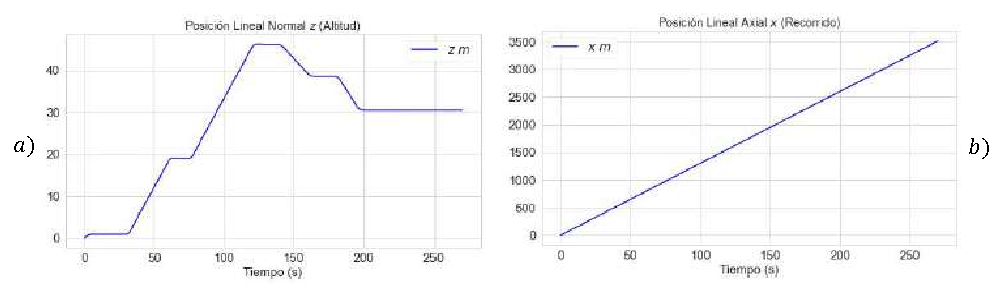
\includegraphics[scale=0.85]{Capitulo3/figs/Simulacion Adaptive Backstepping Longitudinal Posicion 2.pdf}
    \caption{Trayetoria de la Simulación para la dinámica longitudinal de EHEKATL BWB con el controlador Adaptive Backstepping}
    \label{Trayectoria para la dinámica longitudinal de EHEKATL BWB con el controlador Adaptive Backstepping}
\end{figure}

%%%%%%%%%%%%%%%%%%%%%%%%%%%%%%%
\section{Análisis Comparativo}

Cuando se tiene el diseño de diversos sistemas de control de vuelo se puede realizar un análisis comparativo a través de \textbf{indicadores de desempeño} que evalúen las respuesta de cada FCS para diferentes tipos de entrada en términos de estabilidad, precisión y robustez. 

Los indicadores de desempeño a emplear son los siguientes:
\begin{itemize}
    \item \textbf{ISE (Integración del error cuadrático)} En el control de aeronaves, ISE puede usarse para evaluar el desempeño de los FCS de acuerdo en qué tan bien es el seguimiento de la trayectoria deseada. Por tanto, si la aeronave está siguiendo una trayectoria de vuelo específica. 
    \item \textbf{ITSE (Integración del error cuadrático por tiempo)} Toma en cuenta la magnitud del error y el tiempo que le toma converger al sistema. En el control de aeronaves, el ITSE puede evaluar la habilidad del sistema de control para responder rápidamente y minimizar sobre-saltos. Un bajo valor del ITSE coresponde a cambios rápidos y suaves en la condición de vuelo deseada. 
    \item  \textbf{ITAE (Integración del error absoluto por tiempo)} Es utilizado en el control de aeronaves porque minimiza el error absoluto mientras considera el tiempo. Es importante en aviación dónde la precisión y su respuesta en el tiempo son cruciales. Un valor pequeño en ITAE ofrece precisión y rapidez en la respuesta de control. 
    \item \textbf{IAE (Integración del error absoluto)} Es una medida de que tan bien el sistema de control mantiene el error dentro de límites aceptables. En el control de aeronaves, se relaciona con la estabilidad y minimización de las desviación de acuerdo con una trayectoria de vuelo deseada. Un menor valor en IAE sugiere una aeronave más estable y controlable durante el vuelo. 
\end{itemize}

En \ref{indices de desempeño}, se muestran las ecuaciones empleadas para cada índice de desempeño. 
\begin{align}
\label{indices de desempeño}
    ISE = \int e^2  dt \\ \nonumber
    ITSE = \int t e^2 dt \\ \nonumber
    ITAE = \int t |e| dt \\ \nonumber
    IAE = \int |e| dt \\ \nonumber
\end{align}

%\begin{figure}[!h]
%    \centering
%    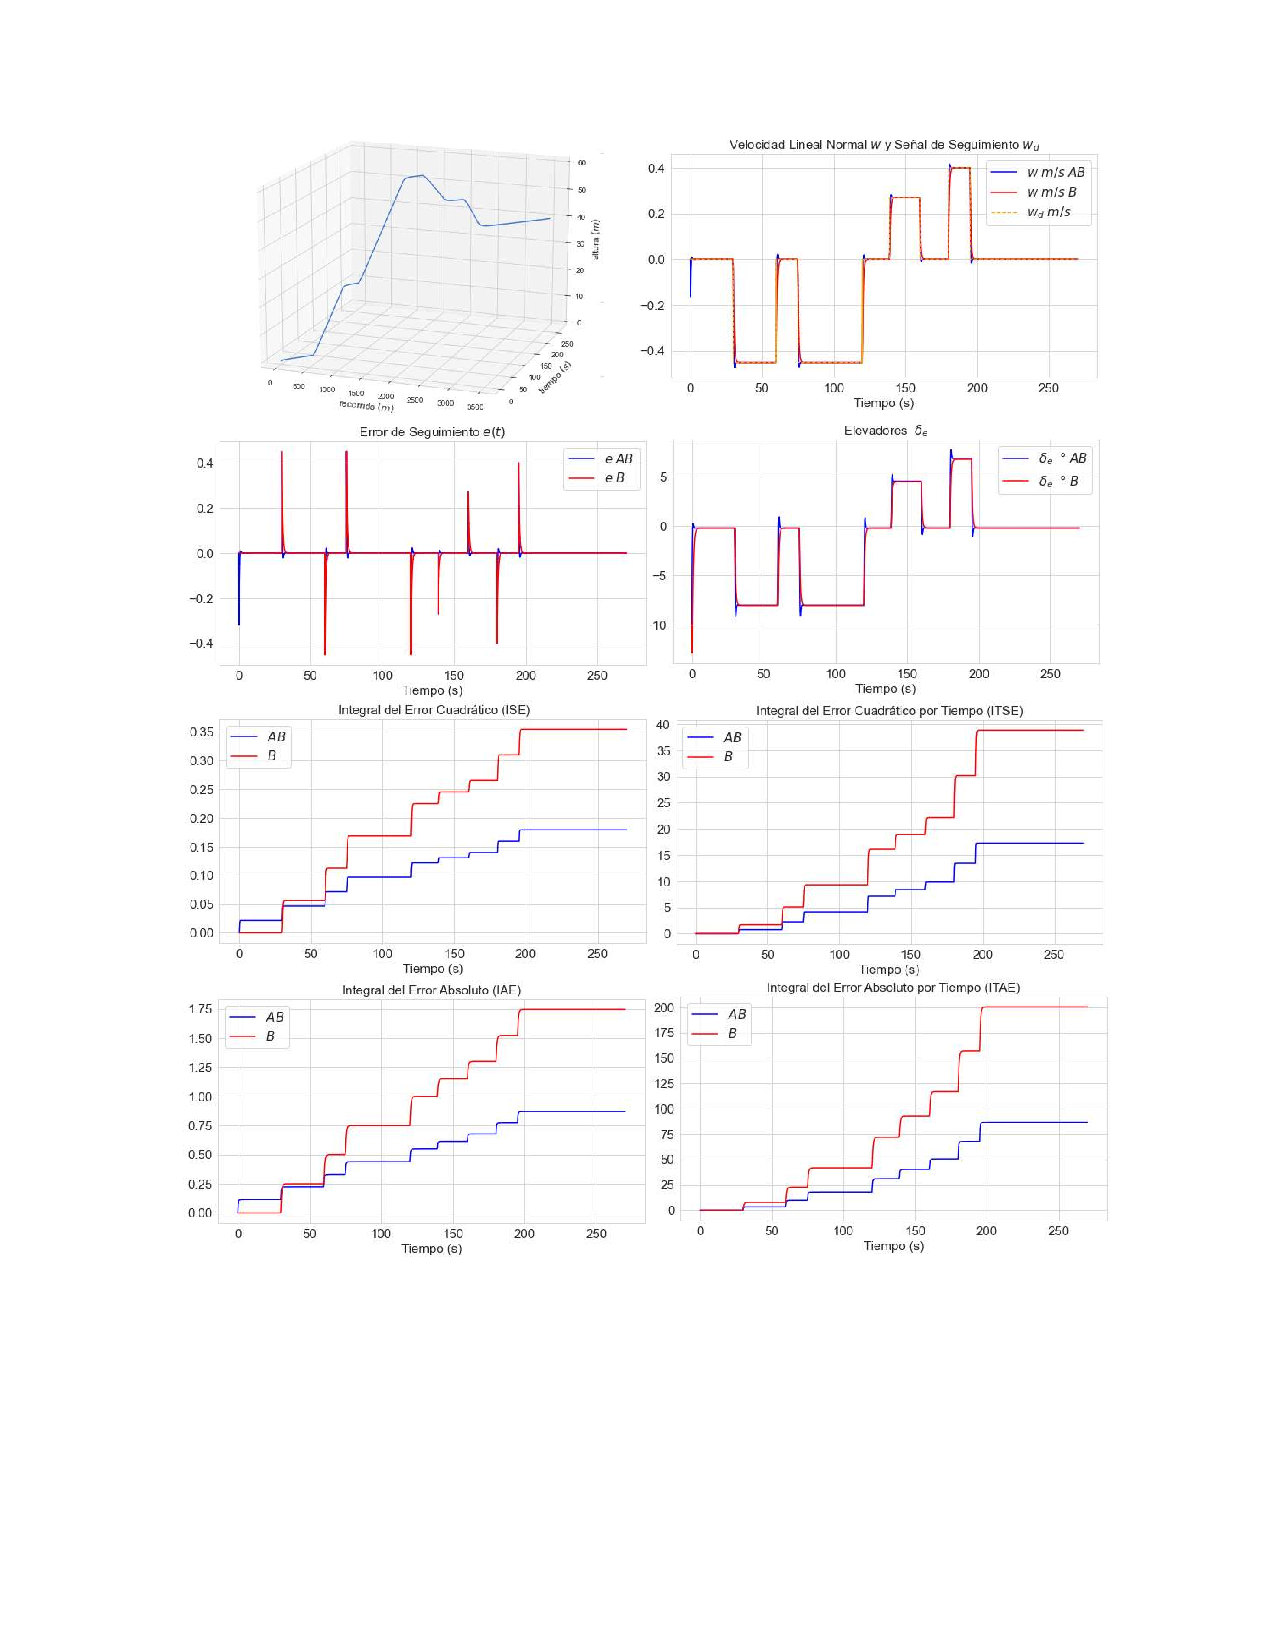
\includegraphics[scale=0.84]{Capitulo3/figs/Simulacion Analsis Comparativo_cropped.pdf}
%    \caption{Simulación - Análisis comparativo con indicadores de desempeño de controladores \textit{Adaptive Backstepping} y \textit{Backstepping} para la dinámica longitudinal de EHEKATL BWB}
%    \label{Simulacion Comparativa}
%\end{figure}
%En \ref{Simulacion Comparativa}, se aplicaron los índices de desempeño para evaluar los controladores Backstepping y Adaptive Backstepping de acuerdo a una trayectoria deseada en el régimen de ascenso en la dinámica longitudinal de EHEKATL BWB. 
%
La simulación que se llevo a cabo fue idéntica a la realizada en \ref{Simulación para la dinámica longitudinal de EHEKATL BWB con el controlador Adaptive Backstepping}.

Los resultados de los índices de desempeño en la evaluación de los controladores Backstepping (\textit{B}) y Adaptive Backstepping (\textit{AB}) se muestran de manera numérica en la Tabla \ref{Indices de desempeño de controladores Backstepping y Adaptive Backstepping} y se establecen las siguientes observaciones.

\begin{table}[!h]
    \caption{Índices de desempeño de controladores Backstepping y Adaptive Backstepping}
    \centering
    \begin{tabular}{|c|c|c|c|c|}
    \hline
    \textbf{Estrategia de Control} & \textbf{ISE} & \textbf{ITSE} & \textbf{ITAE} & \textbf{IAE} \\
    \hline
    Backstepping  & 0.354388888 & 38.8511079 & 200.402469 & 1.74444444 \\
    Adaptive Backstepping & 0.17946439 & 17.2974672 & 86.7001543 & 0.87067341 \\
    \hline
    \end{tabular}
    \label{Indices de desempeño de controladores Backstepping y Adaptive Backstepping}
\end{table}


\bigskip

\textbf{Discusión de los resultados:}
\begin{itemize}
    \item En general, el controlador \textit{AB} ofrece un mejor rendimiento que \textit{B} de acuerdo con los cuatro índices de desempeño. 
    %Puntualmente, los indicadores que no multiplican por el tiempo, \textit{ISE} y \textit{IAE}, muestran al principio de la simulación un error mayor de \textit{AB} únicamente antes de la primer transición de acuerdo con la señal de seguimiento $w_d$. Esto debido a que \textit{AB} muestra una ligera perturbación al inicio de la simulación, situación que no se presenta en \textit{B}. 
    %\item Los indicadores de desempeño que consideran y multiplican por el tiempo, \textit{ITSE} y \textit{ITAE}, no presentan esta situación y muestran un mejor desempeño de \textit{AB} en todas las transiciones, y por tanto, en toda la simulación. 
    Los cuatro indicadores de desempeño muestran una menor acumulación del error de \textit{AB} en cada transición del régimen de ascenso de acuerdo con la señal de seguimiento.
    \item Además, la sintonización de las ganancias de las leyes de control y de adaptación de \textit{AB} fueron menos complejas que la sintonización de las leyes de control de \textit{B}. Es importante señalar que ambos controladores permiten una variedad de diversas aplicaciones en la señal de seguimiento con las mismas ganancias. 
    \item También se observa que para \textit{AB} con las mismas ganancias de las leyes de control, podemos incrementar el peso de las ganancias de las leyes de adaptación y obtener aún mayor precisión y robustez, proceso complejo con el ajuste únicamente de las ganancias en \textit{B}.
\end{itemize}

\section{Discusiones}

El enfoque de control basado en backstepping es una técnica comúnmente utilizada para el diseño de controladores en sistemas dinámicos no lineales. La aplicación de backstepping en el contexto de la aeronave EHEKATL BWB proporciona una metodología sólida para abordar la estabilización y seguimiento de trayectorias en vuelo, considerando las no linealidades del sistema.

La introducción de adaptabilidad en el diseño del controlador mediante el enfoque de backstepping adaptable representa una extensión importante. La capacidad de adaptar el controlador a cambios en los parámetros del sistema o a condiciones de vuelo variables es esencial para garantizar un desempeño óptimo en diversas situaciones operativas.

La evaluación comparativa de los controladores diseñados es crucial para determinar su efectividad y eficiencia en el contexto específico de la EHEKATL BWB. Los indicadores de desempeño proporcionan métricas cuantitativas para evaluar la estabilidad, precisión de seguimiento y respuesta transitoria de los controladores bajo diferentes escenarios de vuelo.


%%%%%%%%%%%%%%%%%%%%%%%%%%%%%%%%%%%%%%%%%%%%%%%%%%%%%%%%
\chapter{Simulaciones de Vuelo en X-PLANE}

X-PLANE es un simulador de vuelo desarrollado por la empresa estadounidense Laminar Research. Es conocido por ser uno de los simuladores de vuelo más realistas y detallados disponibles para computadoras personales.
%
A diferencia de otros simuladores de vuelo, X-PLANE se destaca por su enfoque en la física de vuelo y la aerodinámica precisa. Utiliza un motor de física avanzado que tiene en cuenta una amplia gama de factores, como la forma y características de las aeronaves, las condiciones atmosféricas y la topografía del terreno, para proporcionar una experiencia de vuelo altamente realista.

Las simulaciones de vuelo en X-PLANE permiten validar el trabajo previo (diseño de la aeronave EHEKATL BWB, modelado dinámico y diseño de controladores) en un ambiente virtual que aproxima bien a las condiciones físicas reales. 

El presente capítulo se enfoca en las simulaciones de vuelo en el entorno de X-PLANE llevadas a cabo mediante el uso de la interfaz X-Plane Connect y el desarrollo de controladores Backstepping en PYTHON. Estas simulaciones han sido diseñadas para abordar tres misiones de vuelo cruciales: despegue y ascenso, reconocimiento y descenso y aterrizaje, todas ellas ejecutadas por la aeronave EHEKATL BWB.

\medskip

\textbf{Simulaciones de vuelo de EHEKATL BWB con Backstepping}\\
En la Tabla \ref{Ganancias de controlador Backstepping en X-Plane} se muestran las ganancias utilizadas para el controlador Backstepping en X-PLANE. 
\begin{table}[!h]
    \caption{Ganancias de controlador Backstepping en X-PLANE}
    \centering
    \begin{tabular}{|c|}
    \hline
     Ganancia de la dinámica de cabeceo $K_p$ 0.001 \\
    Ganancia de la dinámica de alabeo $K_r$ 0.001 \\
    Ganancia de control de elevadores $K_e$ 33 \\
    Ganancia de control de alerones $K_a$ 33 \\
    $\tau$ 0.03 \\
    \hline
    \end{tabular}

    \label{Ganancias de controlador Backstepping en X-Plane}
\end{table}

\section{Despegue y Ascenso}
La primera simulación se centra en la fase de despegue y ascenso, dónde la Figura \ref{render ascenso} muestra algunas imágenes de la simulación, mientras la Figura \ref{Misión de Despegue y Ascenso de EHEKATL BWB en el simulador X-PLANE con FCS Bacsktepping} muestra los resultados de la misión respecto al FCS por Backstepping. Durante esta etapa, EHEKATL BWB debe superar la fuerza de gravedad, mientras se eleva desde la pista y adquiere la altitud necesaria para entrar en la fase de crucero. Los FCS por Backstepping desempeñan un papel importante durante el despegue y el ascenso, dónde deben mantener una actitud de cabeceo que permita un régimen de ascenso entre 1$m/s$ y 3$m/s$ con motores al 90$\%$, y dónde la actitud de alabeo debe ser igual o próxima a cero.  A continuación de presentan las discusiones de las simulaciones de la Figura \ref{Misión de Despegue y Ascenso de EHEKATL BWB en el simulador X-PLANE con FCS Bacsktepping} de acuerdo a los resultados obtenidos en X-PLANE.  
\begin{figure}[!h]
    \centering
    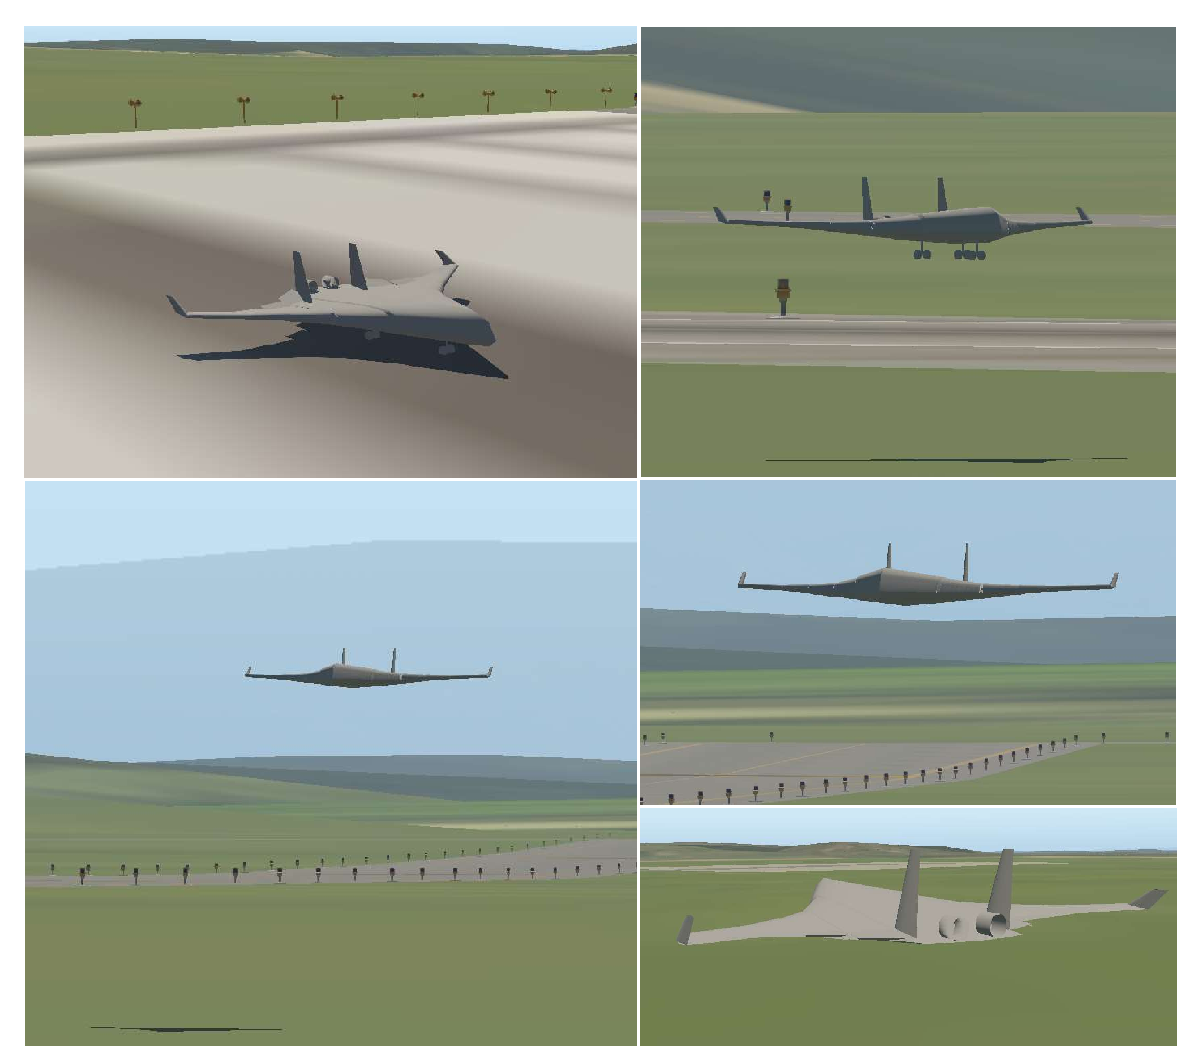
\includegraphics[scale=0.7]{Capitulo3/figs/render ascenso.pdf}
    \caption{Imágenes de simulación de EHEKATL BWB durante el despegue y ascenso en X-PLANE}
    \label{render ascenso}
\end{figure}

\textbf{Discusiones de Resultados:}
\begin{itemize}
    \item En la gráfica a) se muestra la navegación de EHEKATL BWB en 3D de acuerdo con la altitud, la latitud y la longitud. Para esta misión se establece un ángulo de alabeo que se aproxime a cero para mantener un vuelo recto y nivelado. El ángulo de cabeceo mantiene un valor de 1.75$^\circ$ y una potencia de los motores de 90$\%$ para un ROC de 2$m/s$.
\begin{figure}[!h]
    \centering
    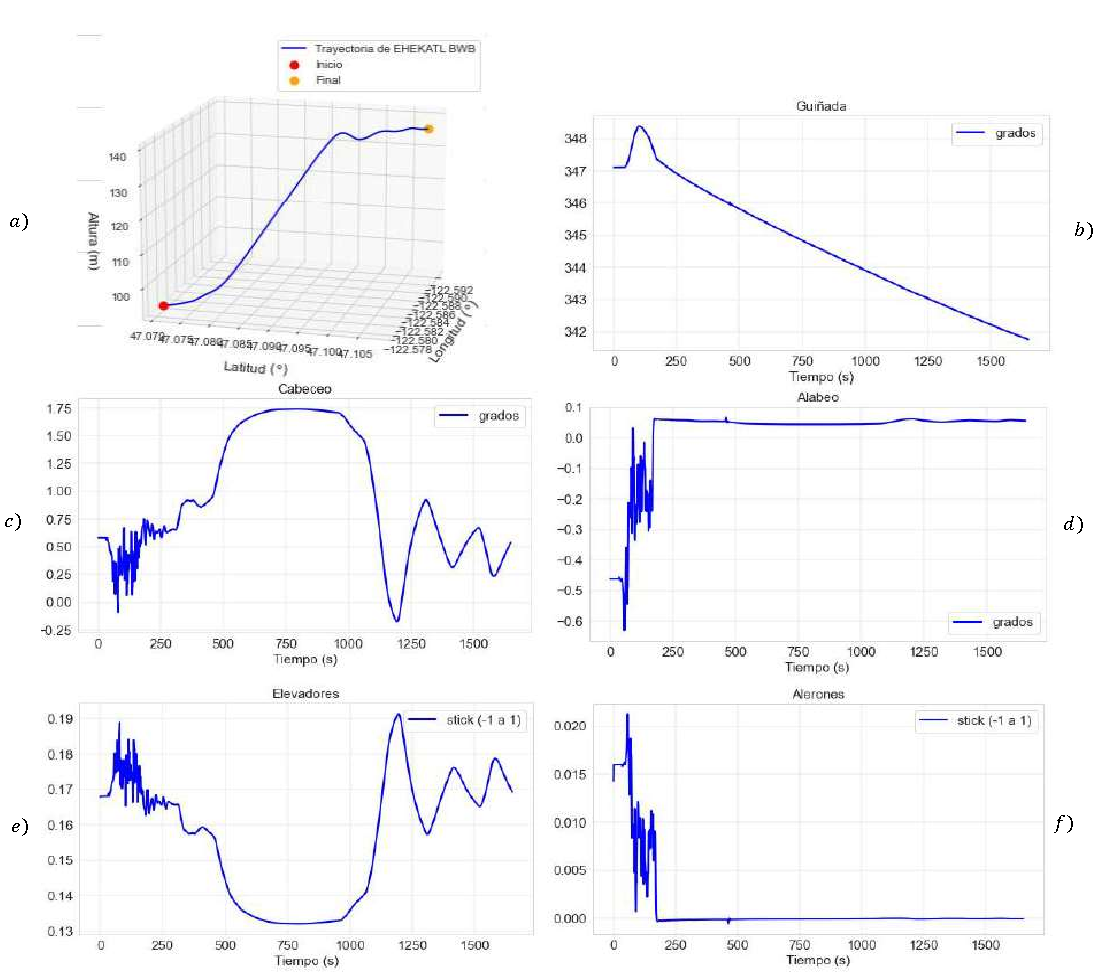
\includegraphics[scale=0.7]{Capitulo3/figs/despegue y ascenso ehekatl 2.pdf}
    \caption{Misión de Despegue y Ascenso de EHEKATL BWB en el simulador X-PLANE con FCS Bacsktepping}
    \label{Misión de Despegue y Ascenso de EHEKATL BWB en el simulador X-PLANE con FCS Bacsktepping}
\end{figure}
    Una vez que se alcanza la altitud de 135m se ajusta la potencia de los motores para mantener la altitud a velocidad constante. 
    En la gráfica b), la guiñada en X-PLANE no refiere al eje $z$ en el sistema de referencia cuerpo de EHEKATL BWB desde una condición inicial inercial, sino más bien a los 360$^\circ$ que se pueden medir con un compás, y de acuerdo a esta coordenadas hacia dónde apunta la nariz de EHEKAT BWB para conocer la orientación del rumbo o dirección. De aquí que la guiñada sea una herramienta de navegación de acuerdo con el rumbo o dirección.
    \item En las gráficas d) y b) se observa que al momento del despegue los alerones generan un momento en alabeo para buscar mantener el vuelo a nivel. Esto debido a las perturbaciones atmosféricas que se presentaron durante el rodaje y de despegue. Ante tales circunstancias, el FCS por Backsepping tiene que controlar los alerones para lograr una respuesta en la orientación del alabeo próxima a cero. Tales peturbaciones atmósfericas permitieron ver la sensibilidad de las aeronaves de ala-integrada a bajas velocidades. Una vez que EHEKATL BWB se sustenta y empieza a ganar altura el valor de alabeo se mantiene constante.
    \item Finalmente, en las gráficas c) y e) se observa la respuesta en cabeceo de acuerdo con la deflexión de los elevadores. Las oscilaciones que se aprecian al principio de la simulación se deben a que el FCS intenta ajusta los elevadores para lograr el ángulo de cabeceo de 1.75$^\circ$ y un ROC constante, sin embargo, la velocidad es muy baja. Durante las simulaciones se observó que EHEKATL BWB empieza a generar sustentación a partir de un Mach de 0.04. Conforme transcurre el tiempo y EHEKATL BWB gana altitud, los elevadores tienen a un valor constante del stick de 0.125 para mantener el ángulo de 1.75$^\circ$. Es importante recordar que la capacidad máxima del stick es de 1 y -1.
    Después del ROC constante de 2$m/s$, se intenta mantener un ROC de 0$m/s$ para mantener un vuelo crucero a altitud constante. Para lograr esta misión se ajusta la potencia de los motores de forma manual. A una potencia de los motores del 45$\%$, con el mismo valor en el FCS para la orientación de cabeceo, se logra la altitud constante con algunas oscilaciones durante el cabeceo.
    \item Finalmente, se mencionan conclusiones importantes durante la simulación en la fase de despegue y ascenso. Los valores asignados para el FCS por Backstepping fueron de 0 para la orientación en alabeo y 6 para la orientación en cabeceo. Estos valores lograron un despegue y ascenso satisfactorios a una potencia de los motores del $90\%$. 
    Cuando se realizó el ajuste en la potencia de los motores fue manteniendo estos mismos valores en el controlador. De aquí surge una opción recomendable para la transición de ascenso al vuelo crucero: una vez que EHEKATL BWB pase del despegue y ascenso, sería necesario reajustar el valor de la orientación del cabeceo para mantener un vuelo a altitud constante. Durante la investigación se demostró que este valor puede ser entre 1 y 3 en la orientación de cabeceo dependiendo de las condiciones atmosféricas.  
\end{itemize}

\section{Reconocimiento}
La segunda simulación está dedicada a una misión de reconocimiento, ver Figuras \ref{render reconocimiento} y \ref{Misión de Reconocimiento de EHEKATL BWB en el simulador X-PLANE con FCS Backstepping}. Aquí, EHEKATL BWB explora su entorno empleando el FCS por Backstepping a una tasa de giro constante hacia la derecha y buscando mantener la actitud en cabeceo. En las primeras tres vueltas se mantiene una potencia de los motores para un ROC de 1$m/s$, posteriormente se ajusta la potencia de los motores para tener un ROC negativo y lograr descender manteniendo los mismos valores en FCS por Backstepping. A continuación se muestran las discusiones de los resultados de simulación de la Figura \ref{Misión de Reconocimiento de EHEKATL BWB en el simulador X-PLANE con FCS Backstepping}.

\begin{figure}[!h]
    \centering
    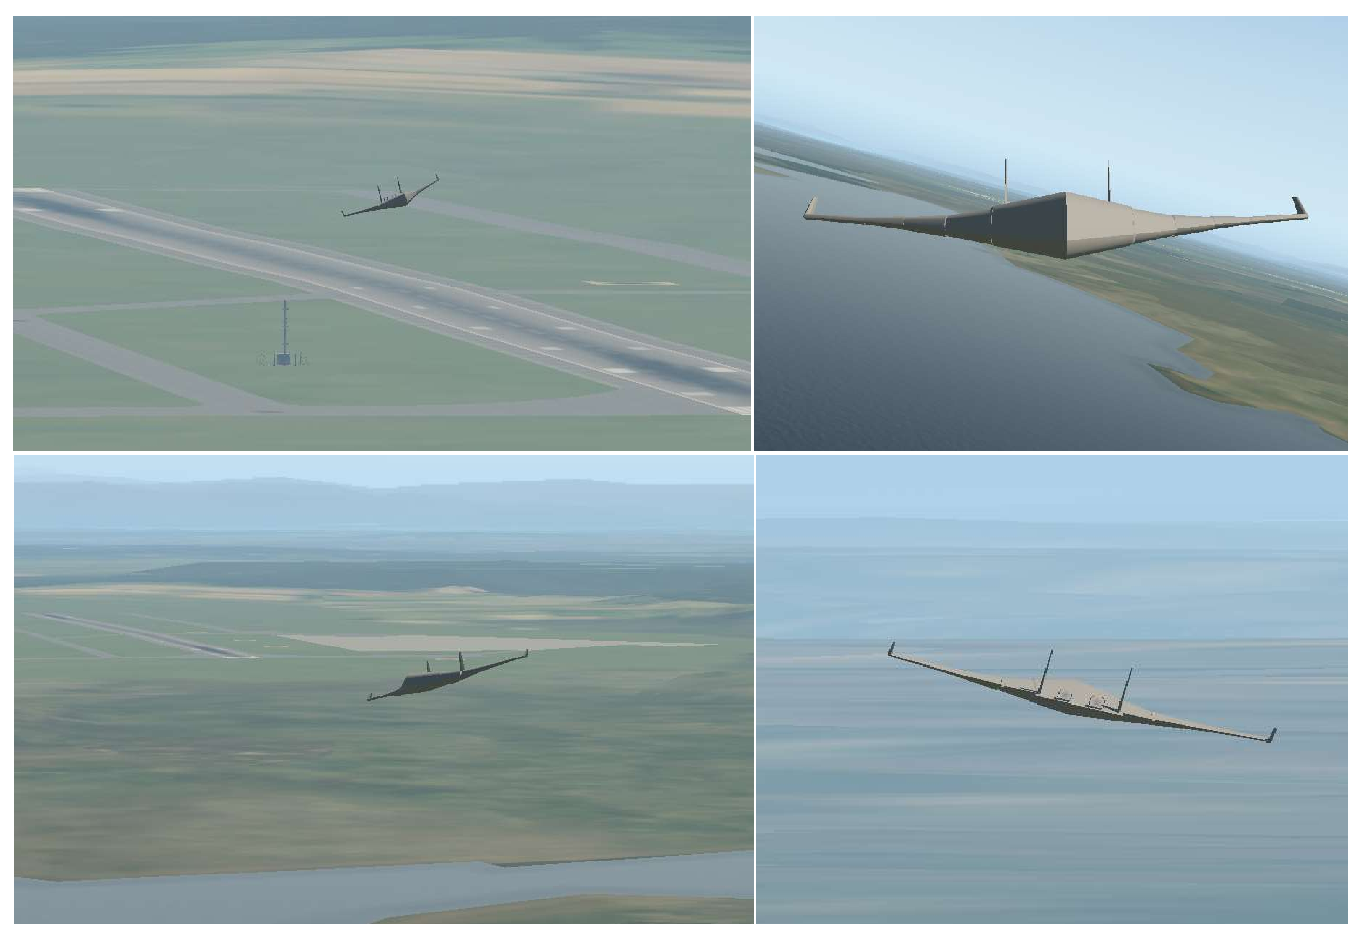
\includegraphics[scale=0.6]{Capitulo3/figs/render reconocimiento.pdf}
    \caption{Imágenes de simulación de EHEKATL BWB durante reconocimiento en X-PLANE}
    \label{render reconocimiento}
\end{figure}

\textbf{Discusión de los Resultados:}
\begin{itemize}
    \item En  La gráfica a) se muestra la trayectoria de EHEKATL BWB en 3D. Se mantiene una tasa de giro hacia la derecha y logra subir su altitud durante 3 vueltas, para después descender en tres vueltas.
    \item La gráfica b) muestra la guiñada en este giro constante yendo de 0$^\circ$ a 360$^\circ$ una y otra vez, durante toda la misión de vuelo.
    \item En la gráfica d) la tasa de giro de alabeo se mantiene constante con una deflexión de los alerones de 0.175 que se observa en la gráfica f), mientras en la gráfica c) se observa una actitud de cabeceo variable, y su respuesta similar en la gráfica e) con la deflexión de sus elevadores.
    \item Los valores asignados en el FCS por Backstepping son de 12 para la orientación de alabeo, 4.5 para la orientación de cabeceo con un ROC de ascenso y de 0.9 en la orientación de cabeceo con un ROC de descenso.
    El valor positivo en el FCS para la orientación de alabeo indica un giro hacia la derecha, mientras un valor negativo indica un giro hacia la izquierda. 
\begin{figure}[!h]
    \centering
    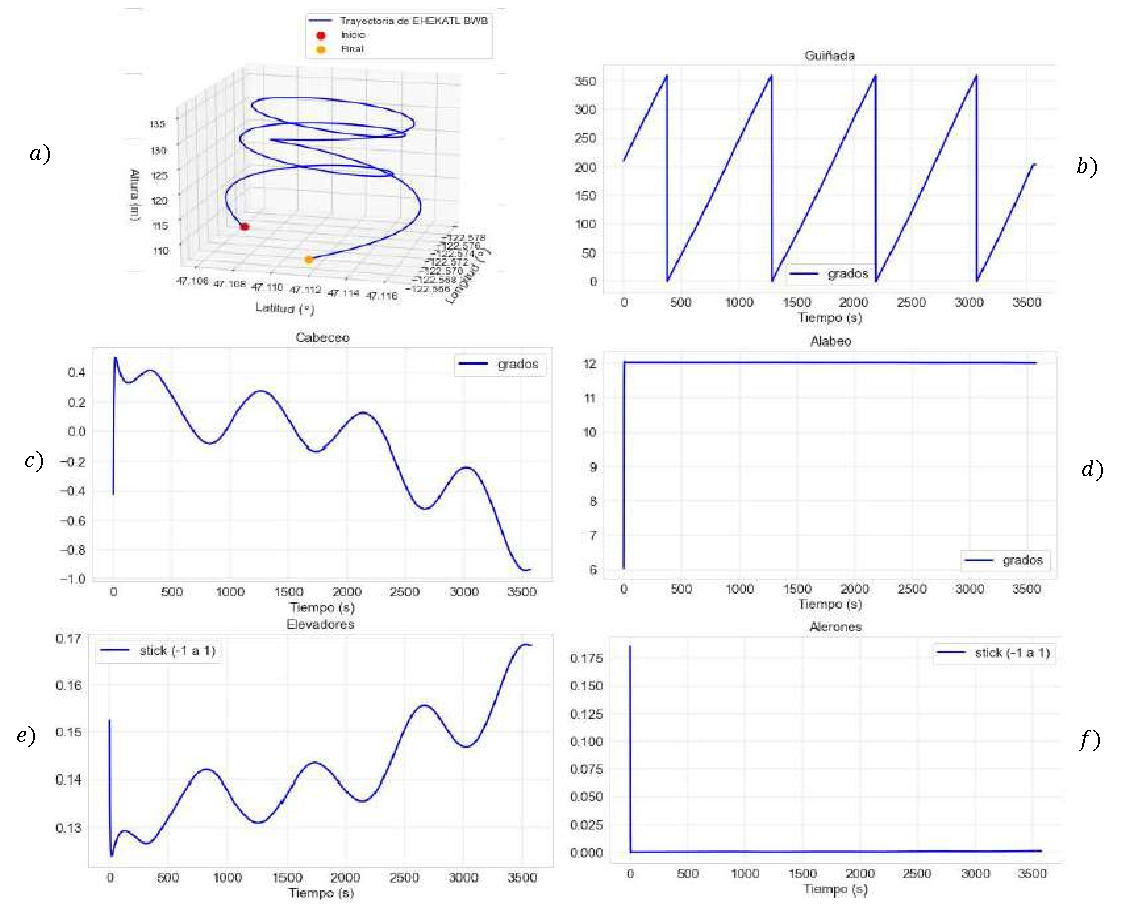
\includegraphics[scale=0.7]{Capitulo3/figs/reconocimiento ehekatl 2.pdf}
    \caption{Misión de Reconocimiento de EHEKATL BWB en el simulador X-PLANE con FCS Backstepping}
    \label{Misión de Reconocimiento de EHEKATL BWB en el simulador X-PLANE con FCS Backstepping}
\end{figure}
\end{itemize}

 
\section{Descenso y Aterrizaje}

El tercer y último escenario de simulación aborda el descenso y aterrizaje, considerada la fase más crítica de vuelo, ver Figura \ref{render landing} y \ref{Misión de Descenso y Aterrizaje de EHEKATL BWB en el simulador X-PLANE con FCS Backstepping}. 
A continuación se muestra la discusión de los resultados de acuerdo con la simulación de la Figura \ref{Misión de Descenso y Aterrizaje de EHEKATL BWB en el simulador X-PLANE con FCS Backstepping}. 

\begin{figure}[!t]
    \centering
    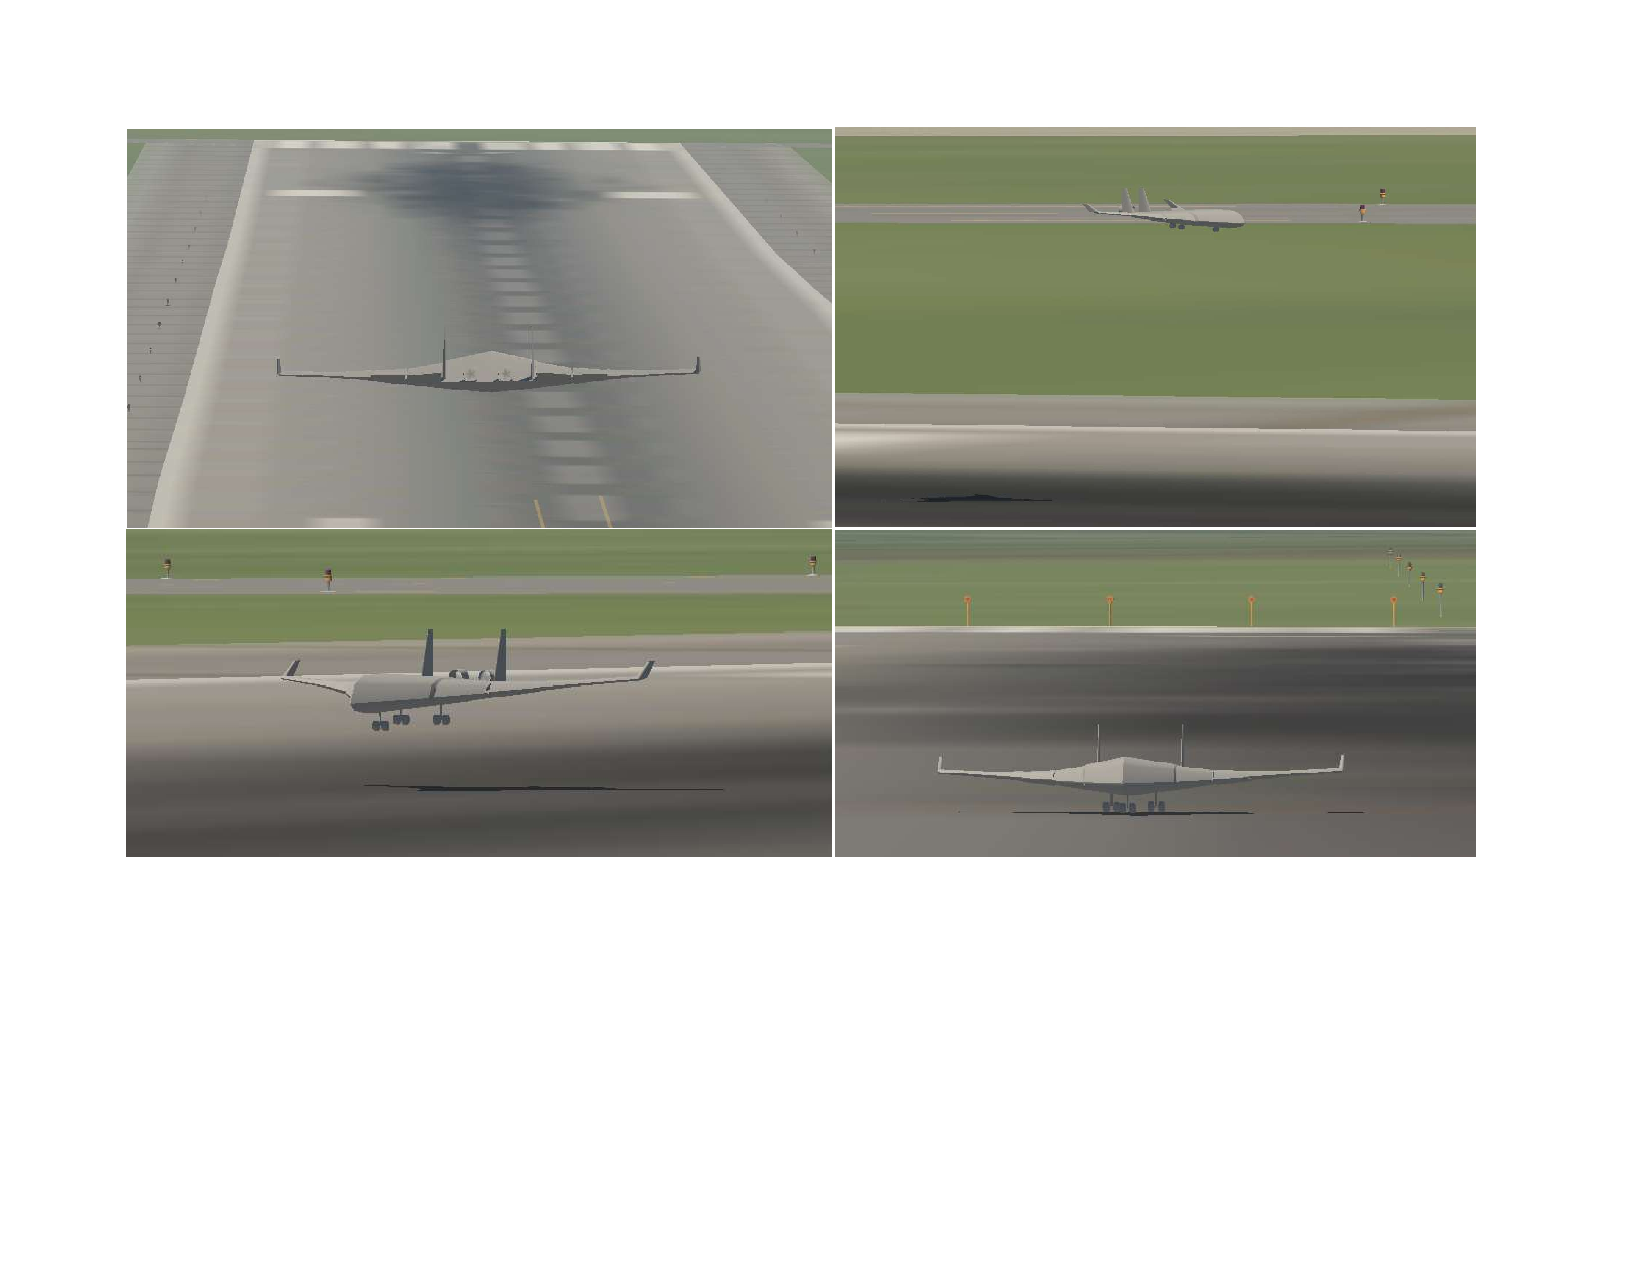
\includegraphics[scale=0.6]{Capitulo3/figs/render aterrizaje_cropped.pdf}
    \caption{Imágenes de simulación de EHEKATL BWB durante descenso y aterrizaje en X-PLANE}
    \label{render landing}
\end{figure}
\begin{figure}[!h]
    \centering
    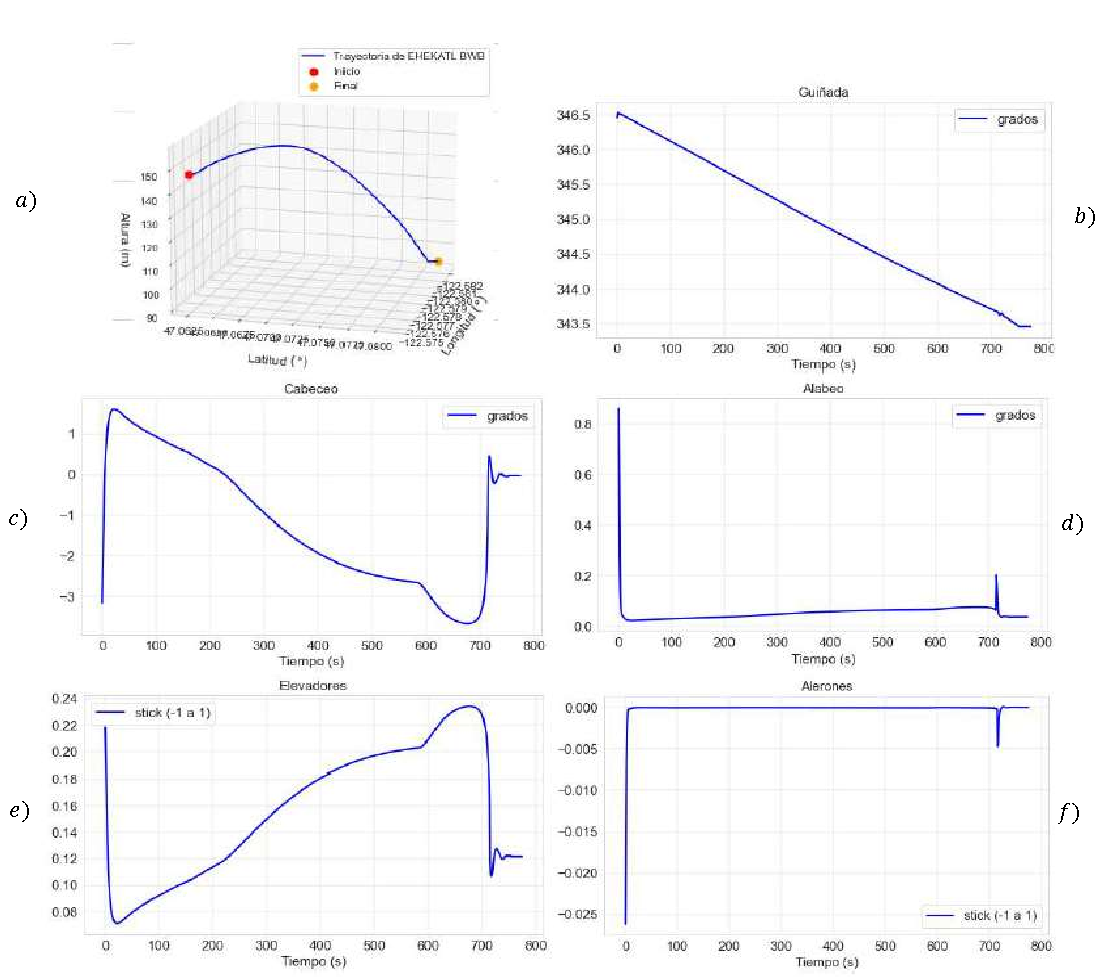
\includegraphics[scale=0.7]{Capitulo3/figs/aterrizaje ehekatl 2.pdf}
    \caption{Misión de Descenso y Aterrizaje de EHEKATL BWB en el simulador X-PLANE con FCS Backstepping}
    \label{Misión de Descenso y Aterrizaje de EHEKATL BWB en el simulador X-PLANE con FCS Backstepping}
\end{figure}

\textbf{Discusiones de Resultados:}
\begin{itemize}
    \item La gráfica a) muestra la trayectoria de EHEKATL BWB en 3D durante el descenso y aterrizaje. Para lograr esta misión tan crucial se configuro el FCS por Backstepping con un valor de alabeo de 0 y un valor de cabeceo de 3. La potencia de los motores se descendió hasta el 5$\%$, para bajar a una velocidad Mach de entre 0.05 y 0.04, que es la velocidad con la que hace contacto en tierra. La parábola de descenso muestra este comportamiento, dónde se aprecia como la curva va descendiendo, pasando de una velocidad de Mach 0.085 en crucero a una velocidad de descenso de 0.05 y tocar tierra a una velocidad de 0.04, dónde se activan los frenos y la aeronave sigue descendiendo su velocidad hasta quedar inmóvil. 
    \item la gráfica b) muestra la guiñada en cuanto a rumbo o dirección, que varia de 346.5 a 343.5.
    \item En las gráfica d) y f) se observa que los alerones se mantienen constantes aunque antes del aterrizaje hacen un pequeño ajuste para lograr el contacto a tierra de manera recta y nivelada. 
    \item En las gráficas c) y e) se observa que el cabeceo disminuye para lograr el descenso desde una velocidad de Mach 0.085 hasta una velocidad de Mach 0.04. 
    Antes de tocar a tierra el controlador logra elevar la nariz para hacer contacto con el tren de aterrizaje trasero, después, se hace el ajuste para descender la nariz y hacer contacto con tierra con el tren delantero.
\end{itemize}

\section{Discusiones} 

La realización de simulaciones de vuelo en X-PLANE durante la fase de ascenso y despegue proporciona una plataforma valiosa para evaluar el rendimiento inicial de la EHEKATL BWB. Los datos obtenidos en esta etapa son esenciales para validar la capacidad de la aeronave para superar la resistencia del aire y lograr una transición fluida hacia el vuelo en crucero.

La fase de reconocimiento en las simulaciones de vuelo en X-PLANE representa un escenario para evaluar la estabilidad y maniobrabilidad durante un giro sostenido. 

La fase de descenso y aterrizaje es una etapa crucial en el ciclo de vuelo de cualquier aeronave. La realización de simulaciones detalladas en X-PLANE durante esta fase permite evaluar la capacidad de la EHEKATL BWB para llevar a cabo maniobras de aproximación y aterrizaje seguras y precisas en una variedad de condiciones ambientales y de tráfico aéreo.

Las simulaciones de vuelo en X-PLANE representan un componente esencial en la validación y refinamiento del diseño de la aeronave EHEKATL BWB. Los resultados obtenidos a partir de estas simulaciones influyen en las decisiones finales de diseño y en la configuración del FCS y navegación a bordo de la aeronave.












